%Este trabalho está licenciado sob a Licença Creative Commons Atribuição-CompartilhaIgual 3.0 Não Adaptada. Para ver uma cópia desta licença, visite http://creativecommons.org/licenses/by-sa/3.0/ ou envie uma carta para Creative Commons, PO Box 1866, Mountain View, CA 94042, USA.

%%%%%%%%%%%%%%%%%%%%%%%%%%%%%%%%%%%%%%%%%%
% ATENÇÃO
%
% POR SEGURANÇA, EVITE EDITAR ESTE ARQUIVO
%
%%%%%%%%%%%%%%%%%%%%%%%%%%%%%%%%%%%%%%%%%

\documentclass[12pt]{book}

\usepackage{tabu}
%\usepackage{ccicons}
%\usepackage{subfiles}

%opções de linguagem
\usepackage[utf8]{inputenc}
\usepackage[portuges]{babel}
\usepackage[T1]{fontenc}

%Indentar primeiro parágrafo de cada seção
\usepackage{indentfirst} 


\usepackage[hmargin=2.5cm,vmargin=2.5cm]{geometry}
%\usepackage[a5paper]{geometry}
\usepackage{amsfonts}
\usepackage{amsmath}
\usepackage{amsthm}
\usepackage{graphics}
\usepackage[normalem]{ulem}
\usepackage{pstricks,pst-plot}
\usepackage[dvips]{graphicx}%
\usepackage{pst-math}
\usepackage{pst-plot}
\usepackage{pst-circ}

\usepackage[pdfborder={0 0 0 [0 0]},colorlinks=true,linkcolor=blue,citecolor=blue,filecolor=blue,urlcolor=blue]{hyperref}


%\usepackage{hyperref}


%%%%%%%%%%%%%%%%%%%%%%%%%%%%%%%
%%%% Exercises and Answers %%%%
%\usepackage[lastexercise]{exercise}
\usepackage[answerdelayed,lastexercise]{exercise}
\usepackage{chngcntr}
\counterwithin{Exercise}{chapter}
\counterwithin{Answer}{chapter}
\renewcommand{\ExerciseHeaderTitle}{({\it \ExerciseTitle})}
\renewcommand{\ExerciseName}{E}
\renewcommand{\ExerciseHeader}{{\textbf{\large\ExerciseName~\ExerciseHeaderNB\ExerciseHeaderTitle\ExerciseHeaderOrigin}}}
\renewcommand{\ExerciseHeader}{\textbf{\ExerciseName\ \ExerciseHeaderNB.}\,}

% change font for answers header
\renewcommand{\AnswerHeader}{\tiny\textbf{\ExerciseName\ \ExerciseHeaderNB.}\smallskip}
% change font for answers list header
\renewcommand{\AnswerListHeader}{{\tiny\textbf{\AnswerListName\
(\ExerciseListName\ \ExerciseHeaderNB)\ ---\ }}}
%%%%%%%%%%%%%%%%%%%%%%%%%%%%%%


\newenvironment{exer}
{\begin{Exercise}}
{\end{Exercise}}

\newenvironment{resp}
{\begin{Answer}\begin{tiny}}
{\end{tiny}\end{Answer}}

\newenvironment{sol}
{\let\oldqedsymbol=\qedsymbol
  \renewcommand{\qedsymbol}{$\Diamond$}
  \begin{proof}[\bfseries\upshape Solução]}
  {\end{proof}
  \renewcommand{\qedsymbol}{\oldqedsymbol}}

%%%%%%%%%%%%%%%%%%%%%%%%%%%%%%
% Exercícios Resolvidos
%%%%%%%%%%%%%%%%%%%%%%%%%%%%%%
\newtheorem{exeresol}{ER}[section]
\newenvironment{resol}
{\let\oldqedsymbol=\qedsymbol
  \renewcommand{\qedsymbol}{$\Diamond$}
  \begin{proof}[\bfseries\upshape Solução]}
  {\end{proof}
  \renewcommand{\qedsymbol}{\oldqedsymbol}}
%%%%%%%%%%%%%%%%%%%%%%%%%%%%%%



\renewcommand{\ExerciseHeaderTitle}{({\it \ExerciseTitle})}
\renewcommand{\ExerciseHeader}{{\textbf{\large\ExerciseName~\ExerciseHeaderNB\ExerciseHeaderTitle\ExerciseHeaderOrigin\medskip}}}

\renewcommand{\AnswerHeader}{\medskip{\textbf{Resposta do exercício \ExerciseHeaderNB}\smallskip}:~}




\newtheorem{teo}{Teorema}
\newtheorem{lem}{Lema}
\newtheorem{prop}{Proposi\c{c}{\~a}o}
\newtheorem{propr}{Propriedade}
\newtheorem{corol}{Corolario}	
\newtheorem{ex}{Exemplo}	
\newtheorem{prob}{Problema}
\newtheorem{obs}{Observa\c{c}{\~a}o}
\newtheorem{defn}{Defini\c{c}{\~a}o}
\newcommand{\senh}{\operatorname{senh}}
\newcommand{\sen}{\operatorname{sen}}



\begin{document}

\frontmatter
\title{Transformadas Integrais}
\date{\today}
\author{}
\maketitle

%Este trabalho está licenciado sob a Licença Creative Commons Atribuição-CompartilhaIgual 3.0 Não Adaptada. Para ver uma cópia desta licença, visite http://creativecommons.org/licenses/by-sa/3.0/ ou envie uma carta para Creative Commons, PO Box 1866, Mountain View, CA 94042, USA.

\chapter*{Organizadores}
\addcontentsline{toc}{chapter}{Organizadores}

\begin{itemize}
\item[] Esequia Sauter - UFRGS
\item[] Fabio Souto de Azevedo - UFRGS
\item[] Irene Strauch - UFRGS
\end{itemize}
%Este trabalho está licenciado sob a Licença Creative Commons Atribuição-CompartilhaIgual 3.0 Não Adaptada. Para ver uma cópia desta licença, visite http://creativecommons.org/licenses/by-sa/3.0/ ou envie uma carta para Creative Commons, PO Box 1866, Mountain View, CA 94042, USA.

\chapter*{Licença}
\addcontentsline{toc}{chapter}{Licença}

Este trabalho está licenciado sob a Licença Creative Commons Atribuição-CompartilhaIgual 3.0 Não Adaptada. Para ver uma cópia desta licença,% visite http://creativecommons.org/licenses/by-sa/3.0/ ou envie uma carta para Creative Commons, PO Box 1866, Mountain View, CA 94042, USA.

%Este trabalho está licenciado sob a Licença Creative Commons Atribuição-CompartilhaIgual 3.0 Não Adaptada. Para ver uma cópia desta licença, visite http://creativecommons.org/licenses/by-sa/3.0/ ou envie uma carta para Creative Commons, PO Box 1866, Mountain View, CA 94042, USA.

\chapter*{Nota dos organizadores}
\addcontentsline{toc}{chapter}{Nota dos organizadores}

Estamos escrevendo este livro de forma colaborativa desde 2011 e, recentemente, decidimos por abrir a colaborações externas. Nosso objetivo é produzir um material didático em nível de graduação de excelente qualidade e de acesso livre pela colaboração entre professores e alunos de universidades, institutos de educação e demais interessados na análise, estudo e aplicação das transformadas integrais nos mais diversos ramos da ciência e da tecnologia.

O sucesso do projeto depende da colaboração! Edite você mesmo o livro, dê sugestões ou nos avise de erros e imprecisões. Toda a colaboração é bem vinda. Saiba mais visitando o site oficial do projeto:
\begin{center}
  %\url{http://www.ufrgs.br/numerico} 
  Ainda não existe
\end{center}

%Nós preparamos uma série de ações para ajudá-lo a participar. Em primeiro lugar, o acesso irrestrito ao livro pode se dar através do \href{http://www.ufrgs.br/numerico}{site oficial do projeto}. Disponibilizamos o livro na versão original em \href{https://github.com/livroscolaborativos/CalculoNumerico/blob/master/main.pdf}{PDF} e versões adaptadas em \href{http://www.ufrgs.br/numerico/book_in_webpage/main.html}{HTML}, \href{http://www.ufrgs.br/numerico/book_in_webpage/main.epub}{EPUB} e \href{http://www.ufrgs.br/numerico/book_in_webpage/slide.pdf}{Slides}. Além disso, o livro está escrito em código \LaTeX disponível em \href{https://github.com/livroscolaborativos/CalculoNumerico}{repositório GitHub público}. 

Nada disso estaria completo sem uma licença apropriada à colaboração. Por isso, escolhemos disponibilizar o material do livro sob licença \href{https://creativecommons.org/licenses/by-sa/3.0/}{Creative Commons Atribuição-CompartilhaIgual 3.0 Não Adaptada (CC-BY-SA 3.0)}. Ou seja, você pode copiar, redistribuir, alterar e construir um novo material para qualquer uso, inclusive comercial. Leia a \href{https://creativecommons.org/licenses/by-sa/3.0/}{licença} para maiores informações.

\vspace{0.5cm}

Desejamos-lhe ótimas colaborações!


%Este trabalho está licenciado sob a Licença Creative Commons Atribuição-CompartilhaIgual 3.0 Não Adaptada. Para ver uma cópia desta licença, visite http://creativecommons.org/licenses/by-sa/3.0/ ou envie uma carta para Creative Commons, PO Box 1866, Mountain View, CA 94042, USA.

\chapter*{Prefácio}
\addcontentsline{toc}{chapter}{Prefácio}

Este livro busca abordar os tópicos de um curso moderno de transformadas de Laplace oferecido a estudantes de matemática, física, engenharias e outros. A ênfase é colocada na formulação e resolução de problemas e interpretação de resultados. Estudam-se a propriedades da transformada de Laplace e seu uso na resolução de equações diferenciais. Evita-se sempre que possível o uso de conhecimentos de variável compleza. Pressupõe-se que o estudante domine conhecimentos e habilidades típicas desenvolvidas em cursos de graduação de cálculo, álgebra linear e equações diferenciais. 







\tableofcontents

%\listoffigures
%\listoftables

\mainmatter


\part{Transformada de Laplace}
%Este trabalho está licenciado sob a Licença Creative Commons Atribuição-CompartilhaIgual 3.0 Não Adaptada. Para ver uma cópia desta licença, visite http://creativecommons.org/licenses/by-sa/3.0/ ou envie uma carta para Creative Commons, PO Box 1866, Mountain View, CA 94042, USA.


\chapter{Introdução}
A modelagem de muitos problemas encontrados na física, química e engenharias tais como massa-mola, ou circuitos em série, envolve funç\~{o}es descontínuas. Um exemplo disso é uma função do tipo chave liga/desliga, que é zero o início do fenômeno, depois sobe instantaneamente a um valor constante durante algum tempo e, finalmente, zero novamente. Métodos analíticos para resolver equações diferenciais, como fator integrante, separação de variáveis, coeficientes a determinar e variação de parâmetros, funcionam bem quando as funções e envolvidas são contínuas. O método que vamos introduzir aqui, chamado de transformada de Laplace, resolve esse tipo de problema. Essencialmente, a transformada de Laplace é uma transformação similar a derivação ou integração, pois leva função em outra função. Alem disso, essa transformação leva a derivada de uma função em produtos da função original. Isso significa que essa transformação leva uma equação diferencial a uma nova equação em termos da funç\~{a}o transformada que é algébrica e pode ser resolvida facilmente. Uma vez que a transformada de Laplace é conhecida, temos que calcular a transformada inversa para obter a solução do problema (\cite{ZILL} and \cite{STRAUCH}). 

Para cursar essas disciplina o estudante deve conhecer técnicas básicas estudadas em disciplinas como Cálculo Diferencial e Integral e Equações Diferenciais. Nesse sentido, propomos alguns exercícios revisando algumas técnicas úteis.
\section{Exercícios de Revisão}
\begin{Exercise}
Use as expressões $\cosh x=\frac{e^x+e^{-x}}{2}$, $\senh x=\frac{e^x-e^{-x}}{2}$, $\cos x=\frac{e^{ix}+e^{-ix}}{2}$ e $\sen x=\frac{e^{ix}-e^{-ix}}{2i}$  para calcular as seguintes integrais:
\begin{itemize}
\item[a)] $\int_{0}^{\infty} \sen(t)e^{-t}dt$
\item[b)] $\int_{0}^{\infty} \cos(wt)e^{-t}dt$
\item[c)] $\int_{0}^{\infty} \sen^2(wt)e^{-t}dt$
\item[d)] $\int_{0}^{\infty} \cos^2(wt)e^{-t}dt$
\item[e)] $\int_{0}^{\infty} \senh(t)e^{-2t}dt$
\item[f)] $\int_{0}^{\infty} \cosh(t)e^{-2t}dt$
\end{itemize}
 
\end{Exercise}
\begin{Answer}
\begin{itemize}
\item[a)] $\frac{1}{2}$
\item[b)] $\frac{1}{w^2+1}$
\item[c)] $\frac{2w^2}{4w^2+1}$
\item[d)] $\frac{2w^2+1}{4w^2+1}$
\item[e)] $\frac{1}{3}$
\item[f)] $\frac{2}{3}$
\end{itemize}
 
\end{Answer}



\begin{Exercise}
 Calcule o valor da integral
$$\int_0^\infty \sen(wt) e^{-st}dt$$
como uma função de $w$ e $s$ sabendo que $s$ e $w$ são constantes reais positivas.
\end{Exercise}
\begin{Answer}
 $\frac{w}{s^2+w^2}$
\end{Answer}


\begin{Exercise} Calcule o valor da integral
$$\int_0^a  e^{-st}dt$$
como uma função de $a$ e $s$ sabendo que $a$ e $s$ são constantes reais positivas.
\end{Exercise}
\begin{Answer}
 $\frac{1-e^{-as}}{s}$
\end{Answer}


\begin{Exercise}  Mostre que se $|x|<1$ então
\begin{itemize}
\item[a)] $\sum_{k=0}^\infty x^k=\frac{1}{1-x}$
\item[b)] $\sum_{k=0}^\infty kx^k=\frac{x}{(1-x)^2}$
\end{itemize}
\end{Exercise}

\begin{Exercise} Use o resultado anterior para resolver os seguintes somatórios
\begin{itemize}
\item[a)]$\sum_{k=0}^\infty e^{-sk}$
\item[b)]$\sum_{k=0}^\infty (-1)^ke^{-sk}$
\item[c)]$\sum_{k=0}^\infty ke^{-sk}$
\end{itemize}
onde $s$ é uma constante real positiva. 
\end{Exercise}
\begin{Answer}
\begin{itemize}
  \item[a)]$\frac{1}{1-e^{-s}}$
  \item[b)]$\frac{1}{1+e^{-s}}$
  \item[c)]$\frac{e^{-s}}{\left(1-e^{-s}\right)^2}$
\end{itemize}
\end{Answer}



\begin{Exercise} Use a técnica de integração por partes para realizar as seguintes integrais:
\begin{itemize}
\item[a)]$\int_0^\infty t e^{-t}dt$
\item[b)]$\int_0^\infty t^2 e^{-t} dt$
\end{itemize}
\end{Exercise}

\begin{Answer}
\begin{itemize}
  \item[a)]$1$
  \item[b)]$2$
  \end{itemize}
\end{Answer}


\begin{Exercise} Calcule a integral
$$I=\int_0^\infty \left|\sen(\pi t)\right| e^{-t}dt$$
escrevendo-o como o somatório
$$I=\sum_{k=0}^\infty(-1)^k\int_{k}^{k+1} \sen(\pi t) e^{-t}dt.$$
\end{Exercise}

\begin{Answer}
\begin{eqnarray*}
I&=&\sum_{k=0}^\infty(-1)^k\int_{k}^{k+1} \sen(\pi t) e^{-t}dt\\
&=&\frac{\pi}{s^2+\pi^2}\sum_{k=0}^\infty\left[e^{-ks}+e^{-(k+1)s}\right]\\
&=&\frac{\pi}{s^2+\pi^2}\frac{1+e^{-s}}{1-e^{-s}}\\
&=&\frac{\pi}{s^2+\pi^2}\frac{e^{s/2}+e^{-s/2}}{e^{s/2}-e^{-s/2}}\\
&=&\frac{\pi}{s^2+\pi^2}\coth(s/2)\\
\end{eqnarray*}

\end{Answer}


%\end{document}

\chapter{Transformada de Laplace}
\section{Definição de transformada de Laplace}{\label{sec_1}}
\begin{defn}Seja $f(t)$ uma função definida nos reais não negativos. Quando a integral
$$
{\mathcal{L}}\{f(t)\}=\int_0^\infty f(t)e^{-st}dt
$$
for convergente, ela será chamada de transformada de Laplace da função $f(t)$.
\end{defn}
A transformada de Laplace $\mathcal{L}\{f(t)\}$ de uma função $f(t)$ é uma função da variável $s$. A notação usual neste contexto é letra minúscula para a função e letra maiúscula para a transformada: $\mathcal{L}\{f(t)\}=F(s)$, $\mathcal{L}\{g(t)\}=G(s)$, $\mathcal{L}\{h(t)\}=H(s)$.
Nos próximos exemplos, vamos aplicar a definição para calcular a transformadas de Laplace de algumas funções.
\begin{ex}\label{ex1} Vamos calcular a transformada de Laplace da função $f(t)=1$:
\begin{eqnarray*}
\mathcal{L}\{1\}&=&\int_0^\infty 1\cdot e^{-st}dt\\
&=&\lim_{a\to\infty}\int_0^a  e^{-st}dt\\
&=&\lim_{a\to\infty} \frac{1-e^{-sa}}{s}.\\
\end{eqnarray*}
O limite $\displaystyle\lim_{a\to\infty}\frac{1-e^{-sa}}{s}$ só existe se $s>0$. Portanto,
\begin{eqnarray*}
\mathcal{L}\{1\}=\frac{1}{s},\qquad s>0.\\
\end{eqnarray*}
\end{ex}
\begin{ex}\label{ex2} A transformada de Laplace da função $f(t)=t$ é calculada fazendo integração por partes:
\begin{eqnarray*}
\mathcal{L}\{t\}&=&\int_0^\infty te^{-st}dt\\
&=&\left.-\frac{te^{-st}}{s}\right|_0^\infty-\int_0^\infty \left(-\frac{e^{-st}}{s}\right)dt .\\
&=&\left.-\frac{te^{-st}}{s}\right|_0^\infty+\frac{1}{s}\int_0^\infty e^{-st}dt .\\
\end{eqnarray*}
onde a notação $\displaystyle\left.-\frac{te^{-st}}{s}\right|_0^\infty$ indica $\displaystyle\lim_{a\to\infty}\left(\left.-\frac{te^{-st}}{s} \right|_0^a\right)$. Observe que, se $s>0$, a primeira parcela do lado direito é zero e a segunda é $\frac{1}{s}\mathcal{L}\{1\}$, isto é,
\begin{eqnarray*}
\mathcal{L}\{t\}&=&\frac{1}{s}\mathcal{L}\{1\}=\frac{1}{s^2},\qquad s>0.\\
\end{eqnarray*}
onde usamos o resultado do exemplo \ref{ex1}.
\end{ex}
\begin{ex} Para calcular a transformada de Laplace da função $f(t)=t^n$ usamos a ideia introduzida no exemplo \ref{ex2} e escrevemos-a em termos da transformada de $t^{n-1}$. Observe primeiro a transformada de $t^2$ e $t^3$
\begin{eqnarray*}
\mathcal{L}\{t^2\}&=&\int_0^\infty t^2e^{-st}dt\\
&=&\left.-\frac{t^2 e^{-st}}{s}\right|_0^\infty-\int_0^\infty \left(-2t\frac{e^{-st}}{s}\right)dt .\\
&=&\frac{2}{s}\int_0^\infty te^{-st}dt=\frac{2}{s}\mathcal{L}\{t\}=\frac{2}{s}\frac{1}{s^2}=\frac{2}{s^3},\qquad s>0
\end{eqnarray*}
\begin{eqnarray*}
\mathcal{L}\{t^3\}&=&\int_0^\infty t^3e^{-st}dt\\
&=&\left.-\frac{t^3 e^{-st}}{s}\right|_0^\infty-\int_0^\infty \left(-3t^2\frac{e^{-st}}{s}\right)dt .\\
&=&\frac{3}{s}\int_0^\infty t^2e^{-st}dt=\frac{3}{s}\mathcal{L}\{t^2\}=\frac{3}{s}\frac{2}{s^3}=\frac{3!}{s^4},\qquad s>0
\end{eqnarray*}
Agora já podemos intuir qual seria a expressão para a transformada de $t^n$:
$$
\mathcal{L}\{t^n\}=\frac{n!}{s^{n+1}},\qquad s>0.
$$
Essa expressão pode ser formalmente demonstrada pelo método de indução matemática (ver exercício \ref{inducao_tn}).
\end{ex}
\begin{ex}{\label{ex_trans_exp}}A transformada de Laplace da função $f(t)=e^{-at}$ pode ser obtida por integração direta:
\begin{eqnarray*}
\mathcal{L}\{e^{-at}\}&=&\int_0^\infty e^{-at}e^{-st}dt\\
&=&\int_0^\infty e^{-(s+a)t}dt\\
&=&\left.\frac{e^{-(s+a)t}}{s+a}\right|_0^\infty=\frac{1}{s+a},\qquad s+a>0
\end{eqnarray*}
\end{ex}
\begin{ex}{\label{ex_trans_sin}}A transformada de Laplace da função $f(t)=\sen(w t)$ pode ser obtida integrando por partes duas vezes:
\begin{eqnarray*}
\mathcal{L}\{\sen(wt)\}&=&\int_0^\infty \sen(wt)e^{-st}dt\\
&=&\left.-\frac{\sen(wt)e^{-st}}{s}\right|_0^\infty-\frac{1}{s}\int_0^\infty \left(w\cos(wt)\right)\left(-e^{-st}\right)dt\\
&=&\frac{w}{s}\int_0^\infty \cos(wt)e^{-st}dt\\
&=&\frac{w}{s}\left(\left.-\frac{\cos(wt)e^{-st}}{s}\right|_0^\infty-\frac{1}{s}\int_0^\infty \left(-w\sen(wt)\right)\left(-e^{-st}\right)dt\right)\\
&=&\frac{w}{s}\left(\frac{1}{s}-\frac{w}{s}\int_0^\infty \sen(wt)e^{-st}dt\right)\\
&=&\frac{w}{s^2}-\frac{w^2}{s^2}\mathcal{L}\{\sen(wt)\} .
\end{eqnarray*}
Observe que obtemos uma equação para $\mathcal{L}\{\sen(wt)\}$:
$$
\mathcal{L}\{\sen(wt)\} =\frac{w}{s^2}-\frac{w^2}{s^2}\mathcal{L}\{\sen(wt)\} .
$$
Resolvemos essa equação e obtemos
$$
\mathcal{L}\{\sen(wt)\}\left(1+\frac{w^2}{s^2}\right)=\frac{w}{s^2},
$$
isto é,
$$
\mathcal{L}\{\sen(wt)\}=\frac{w}{s^2+w^2},\qquad s>0.
$$
\end{ex}
\begin{ex} Vamos agora calcular a transformada de Laplace $\mathcal{L}\{f(t)\}$ de uma função $f(t)$ descontínua definida por partes:
$$
f(t)=\left\{\begin{array}{ll} 0, &0\leq t\leq 4\\ 5, & t> 4.
\end{array}\right.
$$
Aqui usamos a seguinte propriedade de integral: $\int_a^b f(t)dt=\int_a^x f(t)dt+\int_x^b f(t)dt$. Portanto,
\begin{eqnarray*}
\mathcal{L}\{f(t)\}&=&\int_0^\infty f(t)e^{-st}dt\\
&=&\int_0^4 f(t)e^{-st}dt+\int_4^\infty f(t)e^{-st}dt\\
&=&\int_0^4 0\cdot e^{-st}dt+\int_4^\infty 5 e^{-st}dt\\
&=&\left.-\frac{5e^{-st}}{s}\right|_4^\infty=\frac{5e^{-4s}}{s}
\end{eqnarray*}
\end{ex}

\subsection*{Exercícios}
\begin{exer}Calcule a transforma de Laplace da função $f(t)=\cos(wt)$ usando a definição. 
\end{exer}
\begin{exer}Calcule a transforma de Laplace da função $f(t)$ definida por partes:
$$
f(t)=\left\{\begin{array}{ll} 0, &0\leq t\leq 3\\ 1, & 3\leq t\leq 5,\\0,&t>5.
\end{array}\right.
$$
\end{exer}
\begin{exer}{\label{ex_cap_3_1}} Use a definição de transformada de Laplace para calcular as transformadas das funções dadas nos gráficos abaixo:
\begin{center}

\includegraphics{cap_definicao/pics/figura_4}
\includegraphics{cap_definicao/pics/figura_5}
\includegraphics{cap_definicao/pics/figura_6}
\includegraphics{cap_definicao/pics/figura_7}
\includegraphics{cap_definicao/pics/figura_8}\end{center}
\end{exer}
\begin{resp}
 \begin{itemize}
  \item[a)] $\displaystyle F(s)=\frac{k}{s}e^{-sc}$
  \item[b)] $\displaystyle F(s)=\frac{k}{s}\left(1-e^{-sc}\right)$ 
  \item[c)] $\displaystyle F(s)=\frac{k}{s}e^{-sc}\left(1-e^{-sb}\right)$ 
  \item[d)] $\displaystyle F(s)=-\frac{k}{c}\left(\frac{c}{s}e^{-sc}+\frac{1}{s^2}\left(e^{-sc}-1\right)\right)$
  \item[e)] $\displaystyle F(s)=\frac{k}{cs^2}\left(1-2e^{-cs}+e^{-2cs}\right)$
 \end{itemize}
\end{resp}
\begin{exer}Use a definição de transformada de Laplace para calcular as transformadas das funções dadas a seguir:
 \begin{itemize}
  \item[a)] $f(t)=at$
  \item[b)] $f(t)=\left\{\begin{array}{ll}0, & 0\leq t< 2\\2,&  2\leq t< 3\\0,&t>3 \end{array}\right.$
  \item[c)] $f(t)=a^t,~~a>0$
  \item[d)] $f(t)=\cos(wt)$ 
  \item[e)] $f(t)=\cosh(at)$ 
  \item[f)] $f(t)=te^{2t}$ 
  \item[g)] $f(t)=e^{-t+4}$ 
 \end{itemize}
\end{exer}
\begin{resp}
 \begin{itemize}
  \item[a)] $F(s)=\frac{a}{s^2}$
  \item[b)] $F(s)=\frac{2}{s}e^{-2s}\left(1-e^{-s}\right)$ 
  \item[c)] $F(s)=\frac{1}{s-\ln(a)}$
  \item[d)] $F(s)=\frac{s}{s^2+w^2}$ 
  \item[e)] $F(s)=\frac{s}{s^2-a^2}$ 
  \item[f)] $F(s)=\frac{1}{(s-2)^2}$ 
  \item[g)] $F(s)=\frac{e^{4}}{s+1}$ 
  \end{itemize}
\end{resp}
 \begin{exer}\label{inducao_tn}(Princípio da Indução) Mostre que $\displaystyle\mathcal{L}\{t^n\}=\frac{n!}{s^{n+1}}$ seguindo os seguintes passos:
 \begin{itemize}
  \item[a)] Mostre que a fórmula é válida para $n=0,\ 1,\ 2$ e $3$.\footnote{De fato, bastaria mostrar para $n=0$.}
  \item[b)] Mostre que $\displaystyle\mathcal{L}\{t^{n-1}\}=\frac{(n-1)!}{s^{n}}$ é válida, então $\displaystyle\mathcal{L}\{t^n\}=\frac{n!}{s^{n+1}}$ também o é.
 \end{itemize}
 \end{exer}

 
\section{Condição de existência da transformada de Laplace}
A integral que define a transformada de Laplace nem sempre converge e, nesse caso, dizemos que a função não possui transformada de Laplace. As funções $f(t)=e^{t^2}$ e $f(t)=\frac{1}{t}$ são alguns exemplo de funções que não possuem transformada de Laplace. Nessa seção, vamos introduzir uma família de funções que possuem transformada de Laplace. Neste contexto, vamos considerar as funções que são contínuas por partes, ou seja, aquelas que possui um número finito de descontinuidade.
\begin{defn}Dizemos que uma função $f(t)$ é de ordem exponencial $c$ se existem constantes $c$, $M>0$ e $T>0$ tal que $|f(t)|\leq M e^{ct}$ para todo $t>T$. 
\end{defn}
\begin{ex}As funções $f(t)=t^2$, $g(t)=\sen(t)$, $h(t)=e^{-t}$ são de ordem exponencial, pois
$$
|t^2|\leq e^t,\qquad t>0,
$$
$$
|5\cos(t)|\leq e^t,\qquad t>2,
$$
$$
|e^{-t}|\leq e^t,\qquad t>0.
$$
A figura \ref{ordem_exp} ilustra o crescimento de $f$, $g$ e $h$
\begin{figure}[!ht]
\begin{center}

\includegraphics{cap_definicao/pics/figura_1}
\includegraphics{cap_definicao/pics/figura_2}
\includegraphics{cap_definicao/pics/figura_3}\end{center}
\caption{\label{ordem_exp}}
\end{figure}
\end{ex}
\begin{teo}\label{ordem_exp_exist} Se $f(t)$ é integrável em cada intervalo $[a,b]\subset[0,\infty)$ e de ordem exponencial $c$, então a transformada de Laplace de $f(t)$ existe para $s>c$.
\end{teo}
\begin{proof}Como a função $f(t)$ é de ordem exponencial $c$, então existem constantes $c$, $M>0$ e $T>0$ tal que $|f(t)|\leq M e^{ct}$ para todo $t>T$. Assim, se $\hat{T}$ é maior ou igual a $T$, a transformada de Laplace  pode ser escrita como a seguinte soma:
$$
\mathcal{L}\{f(t)\}=\int_0^\infty f(t)e^{-st}dt=\int_0^{\hat{T}} f(t)e^{-st}dt+\int_{\hat{T}}^\infty f(t)e^{-st}dt.
$$
A primeira parcela do lado direito é a integral do produto de duas funções integráveis no intervalo $[0, \hat{T}]$, logo, está bem definido. Agora, como $\hat{T}\geq T$, podemos estimar
\begin{eqnarray*}
\left|\int_{\hat{T}}^\infty f(t)e^{-st}dt\right|&\leq& \int_{\hat{T}}^\infty \left|f(t)\right|e^{-st}dt\leq \int_{\hat{T}}^\infty M e^{ct}e^{-st}dt\\
&=&M \int_{\hat{T}}^\infty e^{-(s-c)t}dt
=\left.\frac{M}{c-s} e^{-(s-c)t}\right|_{\hat{T}}^\infty =\frac{M}{s-c}e^{-(s-c)\hat{T}} ,\qquad s>c.
\end{eqnarray*}
Como $\lim_{\hat{T}\to \infty} \frac{M}{s-c}e^{-(s-c)\hat{T}}=0$, a integral $\int_0^\infty f(t)e^{-st}dt$ converge para todo $s>c$, ou seja, a transformada de Laplace existe neste domínio.
\end{proof}
\begin{obs} O teorema \ref{ordem_exp_exist} apresenta condições suficientes para existência da transformada de Laplace, estas condições não são, no entanto, necessárias. Por exemplo, a função $f(t)=\ln(t)$ não é contínua na origem, sequer é limitada quando $t\to 0+$, mas admite uma Transformada de Laplace.
 \end{obs}
\begin{teo} (Comportamento no infinito) Se a transformada de Laplace de uma função limitada $f(t)$ existe, $F(s)=\mathcal{L}\{f(t)\}$, então
$$
\lim_{s\to\infty}F(s)=0.
$$
\end{teo}
\begin{proof}
 Por definição,
 $$
 F(s)=\int_0^\infty f(t)e^{-st}dt.
 $$
Fazendo $u=st$, temos:
$$
 F(s)=\frac{1}{s}\int_0^\infty f\left(\frac{u}{s}\right)e^{-u}du.
 $$
 Usando o fato que $f$ é limitada, existe $M$ tal que $|f(t)|<M$ e, assim,
$$
| F(s) |\leq \frac{M}{s}\int_0^\infty e^{-u}du = \frac{M}{s}.
 $$ 
 Portanto, $|F(s)|\to 0$ quando $s\to \infty$, o que implica 
 $$
\lim_{s\to\infty}F(s)=0.
$$
\end{proof}

\subsection*{Exercícios}
\begin{exer}Identifique quais funções são integráveis por partes e de ordem exponencial, isto é, se enquadram nas hipóteses do teorema \ref{ordem_exp_exist}.
\begin{itemize}
 \item[a)] $f(t)=e^{30t}$.
 \item[b)] $f(t)=e^{-5t}\cos(t) $.
 \item[c)] $f(t)=\frac{1}{t}$.
 \item[d)] $f(t)=\ln(t)$.
 \item[e)] $f(t)=\frac{1}{t^2}$.
  \item[f)] $f(t)=t^{5}+1$.
  \item[g)] $f(t)=e^{-t^2}$.
  \item[h)] $f(t)=e^{t^2}$.

  
  \item[i)] $
f(t)=\left\{\begin{array}{ll} 0, &0\leq t\leq 3\\ 1, & 3\leq t\leq 5,\\0,&t>5.
\end{array}\right.
$
\end{itemize}


\end{exer}


\section{A transformada inversa de Laplace}
Se $F(s)=\mathcal{L}\{ f(t)\}$ é a transformada de Laplace de $f(t)$, então dizemos que $f(t)=\mathcal{L}^{-1}\{ F(s)\}$ é a transformada inversa de Laplace da função $F(s)$. Essa definição só faz sentido se a transformação definida no conjunto de funções que possuem transformada de Laplace for "bijetora", ou seja, cada função $f(t)$ está relacionada a uma única transformada $F(s)$. É fácil observar que duas funções iguais a partir de $t=0$ possuem a mesma transformada de Laplace. Porém, se duas transformadas são iguais para $s>s_0$, por exemplo, $F(s)=G(s)$, então
$$
\int_0^\infty f(t)e^{-st}dt=\int_0^\infty g(t)e^{-st}dt
$$
ou seja,
$$
\int_0^\infty (f(t)-g(t))e^{-st}dt=0
$$
para cada $s>s_0$. Mas, o fato dessa integral ser nula, não significa que a função $f(t)-g(t)$ é nula. Tome como exemplo a função
$$
h(t)=\left\{\begin{array}{ll} 0,& 0\leq t< 3,\\1,& t= 3,\\0,& t> 3,  \end{array}\right.
$$
que não é nula, mas a integral 
\begin{equation}{\label{eq_int_inv}}
\int_0^\infty h(t)e^{-st}dt=0\qquad \forall s>s_0.
\end{equation}
No entanto, a função $f(t)-g(t)$ não pode ser diferente de zero em um conjunto muito grande. Basta tomar como exemplo uma função que não se anula em um intervalo pequeno:
$$
h(t)=\left\{\begin{array}{ll} 1,& 0\leq t< \epsilon,\\0,& t\geq \epsilon  \end{array}\right.
$$
para $0<\epsilon<<1$. Por menor que seja $\epsilon$, a integral (\ref{eq_int_inv}) não se anula para $s>0$. Existe um conceito que diz que duas funções $h_1(t)$ e $h_2(t)$ são iguais quase-sempre em $[a,b]$ se 
$$
\int_a^b |h_1(t)-h_2(t)|dt=0.
$$
Observe que o módulo no conceito é importante, pois podemos tomar uma função diferente de zero em intervalos grandes e com integral zero, por exemplo,
\begin{equation}{\label{eq_lap_inv}}
h_3(t)=\left\{\begin{array}{ll} 1,& 0\leq t< 1,\\-1,& 1\leq t< 2,\\0,& t\geq 2,  \end{array}\right..
\end{equation}
Observe que a integral (\ref{eq_int_inv}) deverá ser zero para todo $s>s_0$, o que compensa a falta do módulo. Por exemplo, a integral (\ref{eq_int_inv}) aplicada a função (\ref{eq_lap_inv}) não é zero:
\begin{eqnarray*}
\int_0^\infty h_3(t)e^{-st}dt&=&\int_0^\epsilon e^{-st}dt-\int_\epsilon^{2\epsilon} e^{-st}dt\\
&=&\left.\frac{ e^{-st}}{-s}\right|_0^\epsilon-\left.\frac{e^{-st}}{-s}\right|_{\epsilon}^{2\epsilon}\\
&=&\frac{1}{s}-\frac{ e^{-s\epsilon}}{s}-\frac{e^{-s\epsilon}}{s}+\frac{e^{-2s\epsilon}}{s}\neq 0,\qquad s>0.
\end{eqnarray*}
Usando esse conceito, se duas transformadas de Laplace são iguais, as respectivas inversas são iguais quase-sempre. Nesse sentido, uma função que possui transformada de Laplace está contida numa classe de funções que possuem a mesma transformada de Laplace. Se olharmos cada classe de funções como um elemento de um conjunto, então a transformada de Laplace é "bijetora". Isso significa que a transformada inversa está bem definida, mesmo que não escrevemos uma forma integral fechada para ela. Uma forma integral fechada para a transformada inversa de Laplace aparecerá naturalmente na teoria de transformada de Fourier.
Abaixo segue a pequena tabela \ref{tab_1} das transformadas de Laplace que calculamos na seção \ref{sec_1} e suas respectivas inversas. Observe que cada função da segunda coluna representa uma classe de funções iguais quase-sempre. As tabelas \ref{tab_trans_Lap_1} e \ref{tab_trans_Lap_2} do apêndice \ref{ap_A} estão mais completas. As tabelas de transformadas são úteis quando estamos resolvendo uma equação diferencial, pois na prática, consultamos uma tabela para calcular a inversa.
\begin{table}
\begin{small}
\begin{center}
\begin{tabular}{|c|c|}
\hline &\\
$\displaystyle F(s)=\mathcal{L }\{f(t)\} $&$\displaystyle  f(t)=\mathcal{L }^{-1}\{F(s)\}$ \\&\\ 
\hline &\\
$\displaystyle \frac{1}{s} $&$\displaystyle  1$ \\ &\\
\hline &\\
$\displaystyle \frac{1}{s^2} $&$\displaystyle  t$ \\ &\\
\hline &\\
$\displaystyle \frac{1}{s^n}, \qquad (n=1,2,3,...) $&$\displaystyle  \frac{t^{n-1}}{(n-1)!}$ \\ &\\
\hline
\end{tabular}
\begin{tabular}{|c|c|}
\hline &\\
$\displaystyle F(s)=\mathcal{L }\{f(t)\} $&$\displaystyle  f(t)=\mathcal{L }^{-1}\{F(s)\}$ \\&\\ 
\hline &\\
$\displaystyle \frac{a}{a^2+s^2} $&$\displaystyle  \sen(at)$ \\ &\\
\hline &\\
$\displaystyle \frac{1}{s+a} $&$\displaystyle  e^{ -at}$ \\ &\\
\hline
\end{tabular}
\caption{\label{tab_1}}
\end{center}
\end{small}
\end{table}
\begin{ex}Para calcular a transformada inversa da função $F(s)=\frac{10}{100+s^2}$, fixamos $a=10$ na quarta linha da tabela \ref{tab_1} e obtemos
$$
\mathcal{L }^{-1}\left\{ \frac{10}{100+s^2}\right\}=\sen(10t)
$$
\end{ex}
\begin{ex}Da mesma forma, para calcular a transformada inversa da função $F(s)=\frac{1}{s^{30}}$, fixamos $n=30$ na terceira linha da tabela \ref{tab_1} e obtemos
$$
\mathcal{L }^{-1}\left\{ \frac{1}{s^{30}}\right\}=\frac{t^{29}}{29!}.
$$
\end{ex}
\subsection*{Exercícios}

 \begin{exer}Use a tabela \ref{tab_trans_Lap_1} para calcular a transformada Inversa de Laplace das funções:
 \begin{itemize}
  \item[a)] $F(s)=\frac{1}{s^2+4}$
  \item[b)] $F(s)=\frac{1}{s^2-4}$
  \item[c)] $F(s)=\frac{s}{s^2-9}$
  \item[d)] $F(s)=-\frac{s}{s^2+2s+1}-\frac{1}{s^2+2s+1}$ 
  \item[e)] $F(s)=\frac{1}{(s^2+2s+1)(s+1)}$ 
 \end{itemize}
\end{exer}
\begin{resp}
 \begin{itemize}
  \item[a)] $f(t)=\frac{1}{2}\sen(2t)$
  \item[b)] $f(t)=\frac{1}{2}\senh(2t)$ 
  \item[c)] $f(t)=\cosh(3t)$
  \item[d)] $f(t)=-e^{-t}$ 
  \item[e)] $f(t)=\frac{t^2e^{-t}}{2}$ 
  \end{itemize}
\end{resp}

\chapter{A propriedade de linearidade e a transformada da derivada}
\section{Linearidade da transformada de Laplace}
\begin{prop}{\label{prop_lin}}
A transformada de Laplace é uma transformação linear, isto é,
\begin{equation}
\mathcal{L }\left\{\alpha f(t)+\beta g(t)\right\}=\alpha \mathcal{L }\left\{ f(t)\right\}+\beta\mathcal{L }\left\{g(t)\right\}
\end{equation}
sempre que cada uma das transformadas existirem. 
\end{prop}
\begin{proof}
Isso vem direto da propriedade de linearidade da integral:
\begin{eqnarray*}
\mathcal{L }\left\{\alpha f(t)+\beta g(t)\right\}&=&\int_0^\infty \left(\alpha f(t)+\beta g(t)\right)e^{-st}dt\\
&=&\int_0^\infty \alpha f(t)e^{-st}dt+\int_0^\infty\beta g(t)e^{-st}dt\\
&=&\alpha\int_0^\infty  f(t)e^{-st}dt+\beta\int_0^\infty g(t)e^{-st}dt\\
&=&\alpha \mathcal{L }\left\{ f(t)\right\}+\beta\mathcal{L }\left\{g(t)\right\}.
\end{eqnarray*}
\end{proof}
\begin{ex}{\label{ex_trans_sin_2}} A transformada de Laplace da função $f(t)=\sen(wt)$ já foi calculada no exemplo \ref{ex_trans_sin}. Agora vamos calcular novamente usando o resultado do exemplo \ref{ex_trans_exp} e a linearidade da transformada de Laplace. Primeiro recordamos a fórmula de Euler para escrever exponenciais complexas em termos de senos e cossenos:
\begin{eqnarray*}
e^{iwt}&=&\cos(wt)+i\sen(wt)\\
&\hbox{ou}&\\
e^{-iwt}&=&\cos(wt)-i\sen(wt) .
\end{eqnarray*}
As duas expressões podem ser resolvidas em termos do seno e do cosseno para obter
\begin{eqnarray}
{\label{ex_sen}} \sen(wt)&=&\frac{e^{iwt}-e^{-iwt}}{2i}\\
{\label{ex_cos}} \cos(wt)&=&\frac{e^{iwt}+e^{-iwt}}{2}
\end{eqnarray} 
Agora podemos calcular a transformada de Laplace do seno usando a expressão (\ref{ex_sen}).
\begin{eqnarray*}
\mathcal{L }\{\sen(wt)\}&=&\mathcal{L }\left\{\frac{e^{iwt}-e^{-iwt}}{2i}\right\}\\
&=&\frac{1}{2i} \mathcal{L }\left\{ e^{iwt}\right\}-\frac{1}{2i} \mathcal{L }\left\{ e^{-iwt}\right\}\\
&=&\frac{1}{2i}\left( \frac{1}{s-iw}- \frac{1}{s+iw}\right)\\
&=&\frac{1}{2i}\left( \frac{s+iw-(s-iw)}{(s-iw)(s+iw)}\right)\\
&=&\frac{1}{2i}\left( \frac{2iw}{s^2+w^2}\right)\\
&=&\frac{w}{s^2+w^2}
\end{eqnarray*} 
\end{ex}
\begin{exer}Calcule a transformada de Laplace da função $f(t)=\cos(wt)$ usando a propriedade de linearidade \ref{prop_lin}. 
\end{exer}
\begin{exer}Calcule a transformada de Laplace da função $f(t)=e^{at}-e^{bt}$ usando a propriedade de linearidade \ref{prop_lin}. 
\end{exer}
\begin{ex} A transformada de Laplace da função $f(t)=\senh(wt)$ pode ser calculada usando o resultado do exemplo \ref{ex_trans_exp} e as expressões em termos de exponenciais:
\begin{eqnarray}
{\label{ex_senh}} \senh(at)&=&\frac{e^{at}-e^{-at}}{2}\\
{\label{ex_cosh}} \cosh(at)&=&\frac{e^{at}+e^{-at}}{2}.
\end{eqnarray} 
Aplicamos a propriedade \ref{prop_lin} a expressão (\ref{ex_senh}) e temos:
\begin{eqnarray*}
\mathcal{L }\{\senh(at)\}&=&\mathcal{L }\left\{\frac{e^{at}-e^{-at}}{2}\right\}\\
&=&\frac{1}{2} \mathcal{L }\left\{ e^{at}\right\}-\frac{1}{2} \mathcal{L }\left\{ e^{-at}\right\}\\
&=&\frac{1}{2}\left( \frac{1}{s-a}- \frac{1}{s+a}\right)\\
&=&\frac{1}{2}\left( \frac{s+a-(s-a)}{(s-a)(s+a)}\right)\\
&=&\frac{1}{2}\left( \frac{2a}{s^2-a^2}\right)\\
&=&\frac{a}{s^2-a^2}
\end{eqnarray*} 
\end{ex}
\begin{ex}Vamos calcular a tranformada de Laplace da função $f(t)=wt-\sen(wt)$ usando propriedade de linearidade \ref{prop_lin} e o exemplo \ref{ex_trans_sin_2}:
\begin{eqnarray*}
\mathcal{L }\{wt-\sen(wt)\}&=& w\mathcal{L }\left\{ t\right\}- \mathcal{L }\left\{ \sen(wt)\right\}\\
&=&\frac{w}{s^2}-\frac{w}{s^2+w^2}\\
&=&\frac{w(s^2+w^2)-ws^2}{s^2(s^2+w^2)}\\
&=&\frac{w(s^2+w^2)-ws^2}{s^2(s^2+w^2)}=\frac{w^3}{s^2(s^2+w^2)}\\
\end{eqnarray*} 
\end{ex}
\begin{exer}Calcule a transformada de Laplace da função $f(t)=\cosh(at)$ usando a propriedade de linearidade \ref{prop_lin}. 
\end{exer}
\begin{exer}Calcule a transformada de Laplace da função $f(t)=1-\cos(wt)$ usando a propriedade de linearidade \ref{prop_lin}. 
\end{exer}
\begin{obs}A transformada inversa de Laplace também é uma transformação linear, isto é,
\begin{equation}{\label{prop_lin_inv}}
\mathcal{L }^{-1}\left\{\alpha F(s)+\beta G(s)\right\}=\alpha f(t)+\beta g(t).
\end{equation}
Esse resultado é consequência da propriedade de linearidade \ref{prop_lin}:
\begin{eqnarray*}
\mathcal{L }^{-1}\left\{\alpha F(s)+\beta G(s)\right\}&=&\mathcal{L }^{-1}\left\{\alpha \mathcal{L}\{f(t)\}+\beta \mathcal{L}\{g(t)\}\right\}\\
&=&\mathcal{L }^{-1}\left\{\mathcal{L}\left\{\alpha f(t)+\beta g(t)\right\}\right\}\\
&=&\alpha  f(t)+\beta g(t).
\end{eqnarray*}
\end{obs}
\begin{ex}Vamos calcular a tranformada inversa de Laplace da função $F(s)=\frac{2}{s}+\frac{4}{s^2}-\frac{1}{s-1}$ usando propriedade de linearidade \ref{prop_lin_inv} e a tabela \ref{tab_1}:
\begin{eqnarray*}
\mathcal{L }^{-1}\left\{\frac{2}{s}+\frac{4}{s^2}-\frac{1}{s-1}\right\}&=& 2\mathcal{L }^{-1}\left\{\frac{1}{s}\right\}+4\mathcal{L }^{-1}\left\{\frac{1}{s^2}\right\}-\mathcal{L }^{-1}\left\{-\frac{1}{s-1}\right\}\\
&=&2+4t-e^t
\end{eqnarray*} 
\end{ex}
\section{A transformada de Laplace da derivada de uma função}
\begin{prop}{\label{prop_der}}Se $f(t)$ é contínua e de ordem exponencial e $f'(t)$ é contínua por partes para $t\geq 0$, então
\begin{equation}{\label{prop_der_1}}
\mathcal{L }\{f'(t)\}=s \mathcal{L }\{ f(t)\}-f(0).
\end{equation}
\end{prop}
\begin{proof}
Primeiro considere $f(t)$ e $f'(t)$ contínuas nos reais não negativos. Usando integração por partes na definição de transformada de Laplace, temos 
\begin{eqnarray*}
 \mathcal{L}\{f'(t)\}&=&\int_0^\infty e^{-st} f'(t)dt\\
 &=&\left.e^{-st}f(t)\right|_0^\infty-  \int_0^\infty (-se^{-st}) f(t)dt\\
 &=&-f(0)+  s\int_0^\infty e^{-st}f(t)dt\\
 &=&-f(0)+  s\mathcal{L}\{f(t)\}
 \end{eqnarray*}
Se $f'(t)$ for contínua por partes, então separamos as integrais em somas de tal forma que $f'(t)$ seja contínua em cada parcela. Aplicamos integração por partes em cada parcela e obtemos o resultado desejado.
\end{proof}
Considere $f(t)$ e $f'(t)$ contínuas e $f''(t)$ contínua por partes. Então podemos aplicar a expressão \ref{prop_der_1} duas vezes e obter:
\begin{eqnarray}
\nonumber \mathcal{L }\{f''(t)\}&=&s \mathcal{L }\{ f'(t)\}-f'(0)\\ 
\nonumber &=&s\left( s \mathcal{L }\{ f(t)\}-f(0)\right)-f'(0)\\
&=& s^2 \mathcal{L }\{ f(t)\}-sf(0)-f'(0). {\label{prop_der_2}}
\end{eqnarray}
Analogamente, se $f(t),\ f'(t), \cdots, f^{(n-1)}(t)$ são contínuas e $f^{(n)}(t) $ é contínua por partes, então
\begin{eqnarray}{\label{prop_der_n}}
 \mathcal{L }\{f^{(n)}(t)\}= s^n \mathcal{L }\{ f(t)\}-s^{n-1}f(0)-s^{n-2}f'(0)-\cdots-f^{(n-1)}(0). 
\end{eqnarray}
Vamos usar a propriedade \ref{prop_der} da transformada da derivada para calcular transformadas de Laplace.
\begin{ex}Vamos calcular a transformada de $f(t)=\cos(t)$ usando a propriedade \ref{prop_der}. Observe as derivadas:
 $$
 f(t)=\cos(t),\qquad f'(t)=-\sen(t)\qquad\hbox{e}\qquad f''(t)=-\cos(t).
$$
Logo, 
$$
f''(t)=-f(t).
$$
Aplicamos a transformada de Laplace e usamos a propriedade \ref{prop_der}:
$$
s^2F(s)-sf(0)-f'(0)=-F(s).
$$
Usamos o fato que $f(0)=\cos(0)=1$ e $f'(0)=-\sen(0)=0$ e obtemos
$$
s^2F(s)-s=-F(s),
$$
ou seja,
$$
F(s)=\frac{s}{s^2+1},
$$
que confere com o item 14 da tabela \ref{tab_trans_Lap_1}.
\end{ex}
\begin{ex}Agora, vamos calcular a transformada de $g(t)=t\cos(t)$ usando a propriedade \ref{prop_der} da transformada da derivada . Observe as derivadas:
$$
g'(t)=-t\sen(t)+\cos(t)
$$
e
$$
g''(t)=-t\cos(t)-\sen(t)-\sen(t),
$$
ou seja,
$$
g''(t)=-g(t)-2\sen(t).
$$
Aplicamos a transformada de Laplace e usamos a propriedade \ref{prop_der}:
$$
s^2G(s)-sg(0)-g'(0)=-G(s)-2\mathcal{L}\{\sen(t)\}.
$$
Usamos o fato que $g(0)=0\cdot\cos(0)=0$, $g'(0)=-0\cdot \sen(0)+\cos(0)=1$ e $\mathcal{L}\{\sen(t)\}=\frac{1}{s^2+1}$ e obtemos
$$
s^2G(s)-1=-G(s)-\frac{2}{s^2+1},
$$
isto é,
$$
G(s)=\frac{s^2-1}{(s^2+1)^2},
$$
\end{ex}
\section{Aplicação da transformada de Laplace para resolver problemas de valor inicial}
A propriedade da transformada da derivada \ref{prop_der}, juntamente com a propriedade da linearidade \ref{prop_lin}, são importantes para resolver problemas de valor inicial. A ideia é aplicar a transformada de Laplace à equação diferencial e, usando as condições iniciais escrevemos uma equação algébrica para transformada de Laplace da solução, que é chamada de {\bf equação subsidiária}. Em seguida, resolvemos a equação algébrica e calculamos a transformada inversa para obter a solução do problema. Por exemplo, considere o problema de valor inicial de segunda ordem
\begin{eqnarray*}
 y''(t)+ay'(t)+by(t)&=&f(t)\\
y(0)&=&y_0\\
y'(0)&=&y_0'
\end{eqnarray*}
com $a$, $b$, $y_0$ e $y_0'$ constantes. A aplicação da transformada de Laplace nos dá
$$
 \mathcal{L}\{y''(t)\}+a \mathcal{L}\{y'(t)\}+b \mathcal{L}\{y(t)\}= \mathcal{L}\{f(t)\}.
$$
Usando a propriedade \ref{prop_der}, obtemos a seguinte equação subsidiária
$$
 s^2\mathcal{L}\{y(t)\}-sy(0)-y'(0)+a s\mathcal{L}\{y(t)\}-ay(0)+b \mathcal{L}\{y(t)\}= \mathcal{L}\{f(t)\}
$$
ou seja,
$$
 Y(s)=\frac{F(s)+sy_0+y_0'+ay_0}{(s^2+as+b)}
$$
onde $\mathcal{L}\{y(t)\}=Y(s)$ e $\mathcal{L}\{f(t)\}=F(s)$. A solução do problema de valor inicial é  $y(t)=\mathcal{L}^{-1}\{Y(s)\}$.
\begin{ex}Vamos resolver o problema de valor inicial
\begin{eqnarray*}
 y''(t)+y(t)&=&2t\\
y(0)&=&2\\
y'(0)&=&1
\end{eqnarray*}
Primeiro aplicamos a transformada de Laplace na equação diferencial:
 $$
 \mathcal{F}\{y''(t)\}+\mathcal{F}\{y(t)\}=\mathcal{F}\{2t\}
 $$
 Em seguida, usamos a equação \ref{prop_der_2} para obter
 $$
s^2 \mathcal{L }\{ y(t)\}-sy(0)-y'(0)+\mathcal{F}\{y(t)\}=2\mathcal{F}\{t\}.
 $$
 Agora, usamos a notação $\mathcal{L }\{ y(t)\}=Y(s)$ e o fato que $\mathcal{F}\{t\}=\frac{1}{s^2}$ para escrever
 $$
s^2 Y(s)-sy(0)-y'(0)+Y(s)=\frac{2}{s^2}.
 $$
 Obtemos a equação subsidiária quando substituímos $y(0)=2$ e $y'(0)=1$:
 $$
s^2 Y(s)-2s-1+Y(s)=\frac{2}{s^2}.
 $$
 O próximo passo é resolver a equação algébrica para $Y(s)$
 $$
 Y(s)\left(s^2+1\right)=\frac{2}{s^2}+2s+1,
 $$
 isto é,
 $$
 Y(s)=\frac{2}{s^2\left(s^2+1\right)}+\frac{2s}{\left(s^2+1\right)}+\frac{1}{\left(s^2+1\right)}.
 $$
 A solução do problema de valor inicial pode ser escrita como
$$
y(t)=\mathcal{L}^{-1}\left\{\frac{2}{s^2\left(s^2+1\right)}\right\}+\mathcal{L}^{-1}\left\{\frac{2s}{\left(s^2+1\right)}\right\}+\mathcal{L}^{-1}\left\{\frac{1}{\left(s^2+1\right)}\right\}.
$$
 Obtemos as transformadas inversas olhando a tabela \ref{tab_trans_Lap_1} do apêndice \ref{ap_A}, itens 20, 14 e 13:
 $$
 \mathcal{L}^{-1}\left\{\frac{1}{s^2\left(s^2+1\right)}\right\}=t-\sen(t),\qquad w=1\ \hbox{no item 20 da tabela \ref{tab_trans_Lap_1}}, $$
 $$
 \mathcal{L}^{-1}\left\{\frac{s}{\left(s^2+1\right)}\right\}=\cos(t),\qquad w=1\ \hbox{no item 14 da tabela \ref{tab_trans_Lap_1}}
 $$
 e
 $$
 \mathcal{L}^{-1}\left\{\frac{1}{\left(s^2+1\right)}\right\}=\sen(t),\qquad w=1\ \hbox{no item 13 da tabela \ref{tab_trans_Lap_1}}
 $$
 Combinando a propriedade da linearidade \ref{prop_lin}, temos:
 $$
y(t)=2t-2\sen(t)+2\cos(t)+\sen(t)=2t+2\cos(t)-\sen(t)
$$
 \end{ex}
\begin{exer}Resolva o seguinte problema de valor inicial
\begin{eqnarray*}
 y''(t)+2y'(t)+y(t)&=&e^{-t}\\
y(0)&=&-1\\
y'(0)&=&1
\end{eqnarray*}
\end{exer}
\section{Método das frações parciais para calcular transformadas inversas}
Suponha que $P(x)$ e $Q(x)$ são polinômios tais que o grau de $P$ é menor que o grau de $Q$. O polinômio $Q(x)$ pode ser fatorado em polinômios de graus um e dois:
$$
Q(x) = (a_1x + b_1)^{l_1}\cdots (a_nx + b_n)^{l_n}(c_1x^2 + d_1x + e_1)^{p_1}\cdots (c_m x^2 + d_m x + e_m)^{p_m}.
$$
Com isso, podemos encontrar constantes $A_{1,1}, \ldots, A_{n,l_1\cdots l_n}$, $B_{1,1}, \ldots, B_{m,p_1\cdots p_n}$ e $C_{1,1}, \ldots, C_{m,p_1\cdots p_n}$ tais que:
\begin{eqnarray*}
\frac{P(x)}{Q(x)} &=& \sum_{k=0}^{l_1-1} \frac{A_{1,k}}{(a_1x + b_1)^{l1-k}} + \cdots + \sum_{k=0}^{l_n-1}\frac{A_{n,k}}{(a_nx + b_n)^{l_n-k}} \\&+& \sum_{k=0}^{p_1-1} \frac{B_{1,k}x + C_{1,k}}{(c_1 x^2 + d_1 x + e_1)^{p_1-k}} + \cdots + \sum_{k=0}^{p_m-1} \frac{B_{m,k}x + C_{m,k}}{(c_mx^2 + d_mx + e_m)^{p_m-k}}.
\end{eqnarray*}
Esse método é usado para calcular integrais de funções racionais e transformadas inversas de Laplace.
\begin{ex}Para calcular a transformada inversa de Laplace da função racional $F(s)=\frac{1}{(s-1)(s^2-2s-5)}$ usamos o método de frações parciais, ou seja, encontramos $A$, $B$ e $C$ que satisfazem
\begin{eqnarray*}
 F(s)=\frac{1}{(s-1)(s^2+1)}&=&\frac{A}{s-1}+\frac{B+Cs}{s^2+1}\\&=&\frac{A(s^2+1)+(B+Cs)(s-1)}{(s-1)(s^2+1)}\\
 &=&\frac{s^2(A+C)+s(B-C)+A-B}{(s-1)(s^2+1)}.
\end{eqnarray*}
Obtemos o sistema
\begin{eqnarray*}
A+C&=&0\\
B-C&=&0\\
A-B&=&1
\end{eqnarray*}
que tem solução $B=C=-\frac{1}{2}$ e $A=\frac{1}{2}$. Logo,
$$
F(s)=\frac{1}{2}\left(\frac{1}{s-1}-\frac{s+1}{s^2+1}\right).
$$
Escrevendo em uma forma conveniente, temos
$$
F(s)=\frac{1}{2}\left(\frac{1}{s-1}-\frac{s}{s^2+1}-\frac{1}{s^2+1}\right).
$$
A transformada inversa é
$$
f(t)=\frac{1}{2}\left(e^{t}-\cos(t)-\sen(t)\right).
$$
\end{ex}
\begin{exer}Calcule a transformada inversa de Laplace da função 
$$
F(s)=\frac{3s^2-2s-1}{(s-3)(s^2+1)}.
$$
\end{exer}
\section{Exercícios}
\begin{Exercise} Use a linearidade da transformada para calcular a transformada de Laplace das seguintes funções
 \begin{itemize}
  \item[a)] $f(t)=-8t+2\sen(5t)$ 
  \item[b)] $f(t)=-3t^2(t-2)$
  \item[c)] $f(t)=(2t-3)^3$
  \item[d)] $f(t)=\cos(t)^2$
  \item[f)] $f(t)=\sen(t)^3$
  \item[g)] $f(t)=\cosh(t)^3$
 \end{itemize}
 \end{Exercise}
\begin{resp}
 \begin{itemize}
  \item[a)] $F(s)=-\frac{8}{s^2}+\frac{10}{s^2+25}$ 
  \item[b)] $F(s)=-\frac{18}{s^4}+\frac{12}{s^3}$
  \item[c)] $F(s)=\frac{48}{s^4}-\frac{72}{s^3}+\frac{54}{s^2}-\frac{27}{s}$
  \item[d)] $F(s)=\frac{s^2+2}{s^3+4s}$
  \item[e)] $F(s)=\frac{6}{s^4+10s^2+9}$
  \item[f)] $F(s)=\frac{s(s^2-7)}{s^4-10s^2+9}$
 \end{itemize}
\end{resp}
\begin{Exercise} Use a linearidade da transformada inversa para calcular a transformada inversa de Laplace das seguintes funções
 \begin{itemize}
  \item[a)] $F(s)=\frac{2s-8}{s^2+4}$ 
  \item[b)] $F(s)=2s\left(\frac{1}{s^2-4}+\frac{1}{s(s^2-4)}\right)$
 \end{itemize}
 \end{Exercise}
\begin{resp}
 \begin{itemize}
  \item[a)] $f(t)=2\cos(2t)-4\sen(2t)$
  \item[b)] $f(t)=2\cosh(2t)+\senh(2t)$
 \end{itemize}
\end{resp}
\begin{Exercise}Resolva os seguintes itens
\begin{itemize}
 \item[a)] Use a definição para mostrar que $\mathcal{L}\{e^{zt}\}=\frac{1}{s-z}$, $z\in\mathbb{C}$.
 \item[b)] Use a fórmula do item a) para concluir que
 $$
 \mathcal{L}\{e^{(a+ib)t}\}=\frac{s-a+ib}{(s-a)^2+b^2}
 $$
 \item[c)] Use a fórmula de Euler e o item b) para concluir que
 $$
 \mathcal{L}\{e^{at}\cos(bt)\}=\frac{s-a}{(s-a)^2+b^2}
 $$
 e
 $$
 \mathcal{L}\{e^{at}\sen(bt)\}=\frac{b}{(s-a)^2+b^2}
 $$
\end{itemize}
\end{Exercise}
\begin{Exercise} Resolva os seguintes problemas de valor inicial
 \begin{itemize}
  \item[a)] $\displaystyle \left\{\begin{array}{l}y'+2y=1,\\ y(0)=3 \end{array}\right.$
    \item[b)] $\displaystyle \left\{\begin{array}{l}y'+3y=e^t,\\ y(0)=2 \end{array}\right.$
    \item[c)] $\displaystyle \left\{\begin{array}{l}y''+5y'+6y=0,\\ y(0)=1,\\ y'(0)=0 \end{array}\right.$
    \item[d)] $\displaystyle \left\{\begin{array}{l}y''+2y'+y=e^{-t},\\ y(0)=-1,\\ y'(0)=1 \end{array}\right.$
    \item[e)] $\displaystyle \left\{\begin{array}{l}y'' +  y = 2 \cos(t),\\ y(0)=3,\\ y'(0)=4 \end{array}\right.$
    \item[f)] $\displaystyle \left\{\begin{array}{l}y'' +7 y' +12 y = 21 e^{3t},\\ y(0)=3.5, \\ y'(0)=-10 \end{array}\right.$
 \end{itemize}
\end{Exercise}
\begin{resp}
 \begin{itemize}
  \item[a)] $y(t)=\frac{5}{2}e^{-2t}+\frac{1}{2}$
    \item[b)] $y(t)=\frac{1}{4}e^{t}+\frac{7}{4}e^{-3t}$
        \item[c)] $y(t)=3e^{-2t}-2e^{-3t}$
        \item[d)] $y(t)=\frac{1}{2}e^{-t}(t^2-2)$
        \item[e)] $y(t)= t \sen t + 3 \cos t +4 \sen t$
        \item[f)] $y(t)=\frac{e^{3t}}{2} + \frac{5e^{-4t}}{2} + \frac{e^{-3t}}{2}$
        \end{itemize}
\end{resp}
\begin{Exercise} Use a propriedade da transformada da derivada para calcular a transformada das seguintes funções:
\begin{center}

\includegraphics{cap_linear_deriva/pics/figura_1}
\includegraphics{cap_linear_deriva/pics/figura_2}\end{center}
\end{Exercise}
\begin{resp}
 \begin{itemize}
  \item[a)] $F(s)=\frac{1}{s}+\frac{e^{-s}-e^{-2s}}{s^2}$
      \item[b)] $F(s)=\frac{2}{s}+\frac{-e^{-s}+2e^{-3s}-e^{-4s}}{s^2}$
 \end{itemize}
\end{resp}
\begin{Exercise}{\label{frac_parciais}} Realize a expansão em frações parciais das seguintes funções racionais $F(s)$ e calcule as respectivas transformadas inversas $f(t)=\mathcal{L}^{-1}\{F(s)\}$.
\begin{itemize}
\item[a)]$F(s)=\frac{s^2-6s+4}{s^3-3s^2+2s}$
\item[b)]$F(s)=\frac{s^2+s-2}{(s+1)^3}$
\item[c)]$F(s)=\frac{s}{(s+1)^3}$
\item[d)]$F(s)=\frac{5s^2-15s-11}{(s+1)(s-2)^3}$
\item[e)]$F(s)=\frac{3s^2-2s-1}{(s-3)(s^2+1)}$
\item[f)]$F(s)=\frac{s^2+2s+3}{(s^2+2s+2)(s^2+2s+5)}$
\item[g)]$F(s)=\frac{1}{s^2(s-2)}$
\end{itemize}
\end{Exercise}
\begin{resp}
\begin{itemize}
 \item [a)]
 \begin{eqnarray*}
F(s)&=&\frac{s^2-6s+4}{s^3-3s^2+2s}=\frac{s^2-6s+4}{s(s^2-3s+2)}=\frac{s^2-6s+4}{s(s-1)(s-2)}=\frac{A}{s}+\frac{B}{s-1}+\frac{C}{s-2}
\end{eqnarray*}
\begin{eqnarray*}
A&=&\lim_{s\to 0}sF(s)=\lim_{s\to 0}\frac{s^2-6s+4}{(s-1)(s-2)}=\left.\frac{s^2-6s+4}{(s-1)(s-2)}\right|_{s=0}=2\\
B&=&\lim_{s\to 1}(s-1)F(s)=\lim_{s\to 1}\frac{s^2-6s+4}{s(s-2)}=\left.\frac{s^2-6s+4}{s(s-2)}\right|_{s=1}=1\\
C&=&\lim_{s\to 2}(s-2)F(s)=\lim_{s\to 2}\frac{s^2-6s+4}{s(s-1)}=\left.\frac{s^2-6s+4}{s(s-1)}\right|_{s=2}=-2\\
\end{eqnarray*}
\begin{eqnarray*}
\mathcal{L}^{-1}\left\{F(s)\right\}&=&\mathcal{L}^{-1}\left\{\frac{2}{s}+\frac{1}{s-1}-\frac{2}{s-2}\right\}\\
&=&2+e^{t}-2e^{2t},t>0
\end{eqnarray*}
 \item [b)]
\begin{eqnarray*}
F(s)&=&\frac{s^2+s-2}{(s+1)^3}=\frac{A}{(s+1)^3}+\frac{B}{(s+1)^2}+\frac{C}{(s+1)}
\end{eqnarray*}
\begin{eqnarray*}
A&=&\lim_{s\to -1}(s+1)^3F(s)=\lim_{s\to 1}(s^2+s-2)=\left.(s^2+s-2)\right|_{s=-1}=-2\\
\end{eqnarray*}
Conhecendo o valor de $A$, reduzimos o problema a
\begin{eqnarray*}
\frac{s^2+s-2}{(s+1)^3}+\frac{2}{(s+1)^3}=\frac{B}{(s+1)^2}+\frac{C}{(s+1)}
\end{eqnarray*}
Simplificando o lado da esquerda, temos:
\begin{eqnarray*}
\frac{s^2+s-2}{(s+1)^3}+\frac{2}{(s+1)^3}=\frac{s^2+s}{(s+1)^3}=\frac{s(s+1)}{(s+1)^3}=\frac{s}{(s+1)^2}
\end{eqnarray*}
\begin{eqnarray*}
B&=&\lim_{s\to -1}(s+1)^2\frac{s}{(s+1)^2}=-1\\
\end{eqnarray*}
Reduzimos mais uma vez o problema a
\begin{eqnarray*}
\frac{s}{(s+1)^2}+\frac{1}{(s+1)^2}=\frac{C}{s+1}
\end{eqnarray*}
Simplificando o lado da esquerda, temos:
\begin{eqnarray*}
\frac{s}{(s+1)^2}+\frac{1}{(s+1)^2}=\frac{s+1}{(s+1)^2}=\frac{1}{s+1}
\end{eqnarray*}
o que implica $C=1$. Portanto temos:
\begin{eqnarray*}
F(s)&=&\frac{s^2+s-2}{(s+1)^3}=-\frac{2}{(s+1)^3}-\frac{1}{(s+1)^2}+\frac{1}{(s+1)}
\end{eqnarray*}
e, assim,
\begin{eqnarray*}
f(t)&=&e^{-t}\left(-t^2-t+1\right)
\end{eqnarray*}
\item [c)]
\begin{eqnarray*}
F(s)&=&\frac{s}{(s+1)^3}=\frac{s+1}{(s+1)^3}-\frac{1}{(s+1)^3}=\frac{1}{(s+1)^2}-\frac{1}{(s+1)^3}
\end{eqnarray*}
\begin{eqnarray*}
f(t)&=&e^{-t}\left(t-\frac{t^2}{2}\right)
\end{eqnarray*}
 \item [d)]
\begin{eqnarray*}
F(s)&=&\frac{5s^2-15s-11}{(s+1)(s-2)^3}=\frac{A}{s+1}+\frac{B}{(s-2)^3}+\frac{C}{(s-2)^2}+\frac{D}{(s-2)}
\end{eqnarray*}
\begin{eqnarray*}
A&=&\lim_{s\to -1}(s+1)F(s)=-\frac{1}{3}\\
B&=&\lim_{s\to 2}(s-2)^3F(s)=-7\\
\end{eqnarray*}
Obtém-se também
\begin{eqnarray*}
C&=&4\\
D&=&\frac{1}{3}
\end{eqnarray*}
Portanto
$$f(t)=-\frac{1}{3}e^{-t}+\left(-\frac{7}{2}t^2+4t+\frac{1}{3}\right)e^{2t}$$
 \item [e)]
\begin{eqnarray*}
F(s)&=&\frac{3s^2-2s-1}{(s-3)(s^2+1)}=\frac{A}{s-3}+\frac{Bs+C}{s^2+1}
\end{eqnarray*}
\begin{eqnarray*}
A=\lim_{s\to 3}(s-3)F(s)=2\\
\end{eqnarray*}
\begin{eqnarray*}
Bs+C&=&\left(F(s)-\frac{A}{s-3}\right)(s^2+1)\\
&=&\left(\frac{3s^2-2s-1}{(s-3)(s^2+1)}-\frac{2}{s-3}\right)(s^2+1)\\
&=&\left(\frac{3s^2-2s-1-2(s^2+1)}{(s-3)(s^2+1)}\right)(s^2+1)\\
&=&\frac{s^2-2s-3}{(s-3)}=\frac{(s+1)(s-3)}{(s-3)}=s+1
\end{eqnarray*}
Assim, $B=C=1$ e temos
$f(t)=e^{3t}+\cos(t)+\sin(t)$
 \item [f)]
\begin{eqnarray*}
F(s)&=&\frac{s^2+2s+3}{(s^2+2s+2)(s^2+2s+5)}=\frac{As+B}{s^2+2s+2}+\frac{Cs+D}{s^2+2s+5}\\
&=&\frac{(As+B)(s^2+2s+5)+(Cs+D)(s^2+2s+2)}{(s^2+2s+2)(s^2+2s+5)}\\
&=&\frac{(A+C)s^3+(2A+2C+B+D)s^2+(5A+2D+2B+2C)s+(5B+2D)}{(s^2+2s+2)(s^2+2s+5)}\\
\end{eqnarray*}
Comparando coeficientes, temos:
\begin{eqnarray*}
A+C&=&0\\
2A+2C+B+D&=&1\\
5A+2D+2B+2C&=&2\\
5B+2D&=&3
\end{eqnarray*}
\begin{eqnarray*}
A&=&0  \\
B&=&\frac{1}{3}  \\
C&=& 0 \\
D&=&\frac{2}{3}  
\end{eqnarray*}
\begin{eqnarray*}
F(s)&=&\frac{1}{3}\frac{1}{s^2+2s+2}+\frac{2}{3}\frac{1}{s^2+2s+5}\\
&=&\frac{1}{3}\frac{1}{(s+1)^2+1}+\frac{2}{3}\frac{1}{(s+1)^2+2^2}
\end{eqnarray*}
\begin{eqnarray*}
f(t)=\frac{1}{3}e^{-t}\left[\sin(t)+\sin(2t)\right]
\end{eqnarray*}
 \item [g)]
\begin{eqnarray*}
F(s)&=&\frac{1}{s^2(s-2)}=\frac{A}{s}+\frac{B}{s^2}+\frac{C}{s-2}
\end{eqnarray*}
\end{itemize}
\end{resp}

%Este trabalho está licenciado sob a Licença Creative Commons Atribuição-CompartilhaIgual 3.0 Não Adaptada. Para ver uma cópia desta licença, visite http://creativecommons.org/licenses/by-sa/3.0/ ou envie uma carta para Creative Commons, PO Box 1866, Mountain View, CA 94042, USA.

%\documentclass[Main.tex]{subfiles}
%\begin{document}
\chapter{As propriedades de translação e da transformada da integral}

\section{Propriedade de translação no eixo $s$}
Nessa seção vamos calcular a transformada inversa do deslocamento $F(s-a)$ sabendo a transformada inversa de $F(s)$. %O gráfico da figura \ref{fig_trans_1} mostra um exemplo de função com deslocamentos à direita e à esqueda.
%\begin{figure}[!ht]
%\begin{center}

%\psset{xunit =1.5cm,yunit=1cm, linewidth=1\pslinewidth}
% \begin{pspicture}(-4.0,-4.0)(5.0,4.0)
% \psaxes[labels=none]{->}(0,0)(-3.5,-3.5)(4.5,3.5)
%\psplot[linecolor=blue,plotstyle=curve,plotpoints=200]{-1.0}{1.4}{x .2 sub x .2 sub mul x .2 sub mul 2 mul}
%\psplot[linecolor=blue,plotstyle=curve,plotpoints=200]{1.0}{3.4}{x 2.2 sub x 2.2 sub mul x 2.2 sub mul 2 mul}
%\psplot[linecolor=blue,plotstyle=curve,plotpoints=200]{-3.0}{-0.6}{x 1.8 add x 1.8 add mul x 1.8 add mul 2 mul}

%\rput(4.3,.3){$s$}
%\rput(1.0,3.0){$F(s)$}
%\rput(2.7,3.0){$F(s-a)$}
%\rput(-1.2,3.0){$F(s+a)$}

%\end{pspicture}


%\end{center}
%\caption{\label{fig_trans_1}}
%\end{figure}

\begin{propr}{\label{prop_trans_s}}Se $F(s)$ é a transformada de Laplace de $f(t)$, então $e^{at}f(t)$ é a transformada inversa de $F(s-a)$, isto é
\begin{equation}
\mathcal{L}\left\{e^{at}f(t)\right\} =F(s-a),\qquad s>a
\end{equation}
ou
\begin{equation}{\label{eq_trans_s_inv}}
\mathcal{L}^{-1} \left\{F(s-a)\right\} =e^{at}f(t),\qquad s>a.
\end{equation} 
\end{propr}
\begin{proof}É direto da aplicação da definição da transformada de Laplace $F(s-a)$:
\begin{eqnarray*}
 F(s-a)&=&\int_0^\infty f(t)e^{-(s-a)t}dt\\
&=&\int_0^\infty f(t)e^{at}e^{-st}dt\\
&=&\mathcal{L}\left\{e^{at}f(t)\right\}
 \end{eqnarray*}
\end{proof}

Agora vamos calcular algumas transformadas de Laplace usando a propriedade \ref{prop_trans_s}.

\begin{ex}Para calcular a transformada de Laplace de $f(t)=te^{at}$, que é o item 8 da tabela \ref{tab_trans_Lap_1}, usamos o item 2 da mesma tabela,
$$
\mathcal{L}\{t\}=\frac{1}{s^2}=F(s),
$$
e a propriedade de translação \ref{prop_trans_s} com $f(t)=t$:
$$
\mathcal{L}\left\{e^{at}t\right\} =F(s-a)=\frac{1}{(s-a)^2},\qquad s>a
$$
\end{ex}
\begin{ex}Vamos provar o item 25 da tabela \ref{tab_trans_Lap_2},
$$
\mathcal{L}\left\{ \frac{1}{4a^3}(\sen(at)\cosh(at)-\cos(at)\senh(at))\right\}=\frac{1}{s^4+4a^4},
$$
usando os itens 13 e 14 da tabela \ref{tab_trans_Lap_1}:
$$
\mathcal{L}\left\{\frac{1}{a}\sen(at)\right\}=\frac{1}{s^2+a^2},
$$
e
$$
\mathcal{L}\left\{\cos(at)\right\}=\frac{s}{s^2+a^2}.
$$
De fato,
\begin{small}
\begin{eqnarray*}
\mathcal{L}\left\{ \frac{1}{4a^3}(\sen(at)\cosh(at)-\cos(at)\senh(at))\right\}&=&\mathcal{L}\left\{ \frac{1}{4a^3}\left(\sen(at)\frac{e^{at}+e^{-at}}{2}-\cos(at)\frac{e^{at}-e^{-at}}{2}\right)\right\}\\
&=&\mathcal{L}\left\{ \frac{1}{8a^3}\left(e^{at}\left( \sen(at)-\cos(at)\right)+e^{-at}\left(\sen(at)+\cos(at)\right)\right)\right\}\\
&=&\frac{1}{8a^3}\left[ \mathcal{L}\left\{ \left(e^{at}\left( \sen(at)-\cos(at)\right)\right\}+\mathcal{L}\left\{e^{-at}\left(\sen(at)+\cos(at)\right)\right)\right\}\right]\\
&=&\frac{1}{8a^3}\left[\frac{a}{(s-a)^2+a^2}-\frac{s-a}{(s-a)^2+a^2}\right.\\&&\hspace{40pt}+\left.\frac{a}{(s+a)^2+a^2}+\frac{s+a}{(s+a)^2+a^2}\right]\\
&=&\frac{1}{8a^3}\left[\frac{8a^3}{\left((s-a)^2+a^2\right)\left((s+a)^2+a^2\right)}\right]\\
&=&\frac{1}{s^4+4a^4}
\end{eqnarray*}
\end{small}
\end{ex}
\begin{prob}Use a propriedade \ref{prop_trans_s} e as tabelas \ref{tab_trans_Lap_1} e \ref{tab_trans_Lap_2} para calcular as seguintes transformadas de Laplace
\begin{itemize}
 \item[a)] $\displaystyle \mathcal{L}\left\{\frac{1}{(n-1)!}t^{n-1}e^{at}\right\}$\qquad (usando o item 3 da tabela)
 \item[b)] $\displaystyle \mathcal{L}\left\{\frac{1}{w}\sen(wt)e^{at}\right\}$\qquad (usando o item 13 da tabela)
\end{itemize}

\end{prob}
\begin{ex}Vamos calcular a transformada de Laplace de $f(t)=e^{-t}\cosh(2t)$ usando a propriedade \ref{prop_trans_s} e a tabela \ref{tab_trans_Lap_1}. Primeiro observe o item 16 da tabela com $a=2$:
$$
\mathcal{L}\{\cosh(2t)\}=\frac{s}{ s^2-4}=F(s).
$$
Agora use a propriedade da translação no eixo $s$
\begin{equation}
\mathcal{L}\left\{e^{-t}\cosh(2t)\right\} =F(s+1)=\frac{s+1}{ (s+1)^2-4},\qquad s>-1
\end{equation}


\end{ex}
\begin{prob}Use a propriedade \ref{prop_trans_s} e as tabelas \ref{tab_trans_Lap_1} e \ref{tab_trans_Lap_2} para calcular as seguintes transformadas de Laplace
\begin{itemize}
 \item[a)] $\displaystyle \mathcal{L}\left\{\senh(2t)\cos(t)\right\}$
 \item[b)] $\displaystyle \mathcal{L}\left\{(4+t^2)e^t\right\}$
\end{itemize}
\end{prob}
\begin{ex}
 \item[a)] Agora vamos usar a propriedade \ref{prop_trans_s} e o item 15 da tabela \ref{tab_trans_Lap_1} para calcular a transformadas inversa de Laplace da função $F(s)=\frac{1}{s^2-2s-3}$. Primeiro escrevemos $F(s)$ numa forma conveniente:
$$
F(s)=\frac{1}{s^2-2s-3}=\frac{1}{(s-1)^2-1-3}=\frac{1}{(s-1)^2-4}.
$$
Observe no item 16 da tabela que $\displaystyle\mathcal{L}\left\{\frac{1}{2}\senh(2t)\right\}=\frac{1}{ s^2-4}=G(s)$ e, também, pela propriedade da translação no eixo $s$ dada na equação (\ref{eq_trans_s_inv})
$$
\mathcal{L}^{-1}\{F(s)\}=\mathcal{L}^{-1}\{G(s-1)\}=\frac{1}{2}e^{t}\senh(2t).
$$
\end{ex}

\begin{prob}Encontre $f(t)$ dado que $F(s)$ usando as tabelas e as propriedades
\begin{itemize}
 \item[a)] $F(s)=\frac{s}{(s+1)^2+1}$
\item[b)] $F(s)=\frac{s-1}{(s^2-2s+5)(s^2-2s+10)}$
\end{itemize}
\end{prob}
\section{Aplicação: Oscilador Harmônico}
Uma mola elástica com uma extremidade fixada prende um corpo de massa $m$ na outra extremidade (veja figura (\ref{massa-mola})). Conside que o corpo esteja sujeito a uma força de atrito proporcional a velocidade com constante de amortecimento $\gamma$ e a que mola obedeça a lei de Hooke com constante $k$.
\begin{figure}[!ht]
\begin{center}
\psset{xunit =1cm,yunit=1cm, linewidth=1\pslinewidth}
 \begin{pspicture}(-0.5,1.0)(8.0,5.0)
\psset{linecolor=blue}

\psline(0.0,1.47)(0.0,5.0)

\coil(0.0,2.5)(2.0,2.5){}
\coil(2.0,2.5)(4.0,2.5){}
\psline(4.0,1.5)(4.0,3.5)
\psline(4.0,1.5)(6.0,1.5)
\psline(4.0,3.5)(6.0,3.5)
\psline(6.0,1.5)(6.0,3.5)

\psline(0.0,1.5)(-.3,1.8)
\psline(0.0,2.0)(-.3,2.3)
\psline(0.0,2.5)(-.3,2.8)
\psline(0.0,3.0)(-.3,3.3)
\psline(0.0,3.5)(-.3,3.8)
\psline(0.0,4.0)(-.3,4.3)
\psline(0.0,4.5)(-.3,4.8)
\psline(0.0,5.0)(-.3,5.3)

\psline{->}(0.0,1.47)(7.5,1.47)

\psline(5.0,1.37)(5.0,1.57)

\rput(7.8,1.17){$y(t)$}
\rput(5.0,1.17){$0$}

\end{pspicture}
\end{center}
\caption{\label{massa-mola}}
\end{figure} 

Seja $y(t)$ o deslocamento do corpo da sua posição de equilíbrio estático em função do tempo $t$. A equação do movimento é obtida a partir da segunda lei de Newton:
$$
ma=\sum_i f_i,
$$
onde $a=y''(t)$ é a aceleração e $\sum_i \vec{f}_i$ representa a soma de todas as forças. No caso tratado aqui, existem apenas três forças, a saber:
\begin{itemize}
 \item[i)] a força da mola, que é proporcional ao descocamento (lei de Hooke), com constante de proporcionalidade $k$, $f_1=-k y(t)$,
 \item[ii)] a força de atrito, que é proporcional a velocidade, com constante de amortecimento $\gamma$, $f_2=-\gamma y'(t)$, e
 \item[iii)] a força externa, $f_3(t)=f(t)$
\end{itemize}
Logo,
$$
my''(t)=f_1+f_2+f_3=-ky(t)-\gamma y'(t)+f(t),
$$
ou seja, a equação para o deslocamento $y(t)$ é dada por
\begin{equation}{\label{eq_massa_mola}}
my''(t)+\gamma y'(t)+ky(t)=f(t).
\end{equation}
O modelo fica completo quando impomos as condições iniciais $y(0)=y_0$ e $y'(0)=y_0'$. 

Agora, vamos usar o método da transformada de Laplace para resolver a equação. Aplicamos a transformada de Laplace na equação (\ref{eq_massa_mola}) e obtemos:
$$
m\mathcal{L}\{y''(t)\}+\gamma \mathcal{L}\{y'(t)\}+k\mathcal{L}\{y(t)\}=\mathcal{L}\{f(t)\}.
$$
Aplicamos a propriedade \ref{prop_der} e obtemos
$$
ms^2\mathcal{L}\{y(t)\}-msy(0)-my'(0)+\gamma s\mathcal{L}\{y(t)\}-\gamma y(0)+k\mathcal{L}\{y(t)\}=\mathcal{L}\{f(t)\}.
$$
Impomos as condições iniciais para obter a seguinte equação subsidiária:
$$
ms^2Y(s)-msy_0-my_0'+\gamma sY(s)-\gamma y_0+kY(s)=F(s),
$$
onde $F(s)=\mathcal{L}\{f(t)\}$ e $Y(s)=\mathcal{L}\{y(t)\}$. Resolvemos a equação para $Y(s)$:
$$
Y(s)=\frac{F(s)+msy_0+my_0'+\gamma y_0}{ms^2+\gamma s +k}.
$$
A solução do problema pode ser representado por $y(t)=\mathcal{L}^{-1}\{Y(s)\}$. 

O sistema massa mola pode ser classificado das seguintes formas:
\begin{itemize}
 \item[i)] Oscilador harmonico forçado: quando a força externa não é nula.
 \item[ii)] Oscilador harmônico livre: quando não há força externa, ou seja, $f(t)=0$, o que implica em $F(s)=0$. Nesse caso
$$
Y(s)=\frac{msy_0+my_0'+\gamma y_0}{ms^2+\gamma s +k}.
$$
\item[iii)] Oscilador harmônico subamortecido: quando $\gamma^2< 4mk$. No caso $F(s)=0$, temos:
$$
Y(s)=\frac{msy_0+my_0'+\gamma y_0}{ms^2+\gamma s +k}=\frac{msy_0+my_0'+\gamma y_0}{m\left(s+\frac{\gamma}{2m}\right)^2-\frac{\gamma^2}{4m} +k},
$$
onde $-\frac{\gamma^2}{4m} +k>0$. Olhando os itens 13 e 14 da tabela de transformada \ref{tab_trans_Lap_1} e combinando com a propriedade \ref{prop_trans_s}, concluímos que as soluções são são senos e cossenos multiplicados por exponenciais.
\item[iv)] Oscilador harmônico superamortecido: quando $\gamma^2> 4mk$. No caso $F(s)=0$, temos:
$$
Y(s)=\frac{msy_0+my_0'+\gamma y_0}{ms^2+\gamma s +k}=\frac{msy_0+my_0'+\gamma y_0}{m\left(s+\frac{\gamma}{2m}\right)^2-\frac{\gamma^2}{4m} +k},
$$
onde $-\frac{\gamma^2}{4m} +k<0$. Olhando os itens 15 e 16 da tabela de transformada \ref{tab_trans_Lap_1} e combinando com a propriedade \ref{prop_trans_s}, concluímos que as soluções são são senos e cossenos hiperbólicos multiplicados por exponenciais, ou seja, somas de exponenciais puras (lembre-se que $\displaystyle 2\senh(at)=e^{at}-e^{-at}$ e $\displaystyle2\cosh(at)=e^{at}+e^{-at}$).
\item[v)] Oscilador harmônico criticamente amortecido: quando $\gamma^2= 4mk$. No caso $F(s)=0$, temos:
$$
Y(s)=\frac{msy_0+my_0'+\gamma y_0}{ms^2+\gamma s +k}=\frac{msy_0+my_0'+\gamma y_0}{m\left(s+\frac{\gamma}{2m}\right)^2},
$$
Olhando para o item 3 da tabela de transformada \ref{tab_trans_Lap_1} e combinando com a propriedade \ref{prop_trans_s}, concluímos que as soluções são polinômios multiplicados por exponenciais.
\item[vi)] Oscilador harmônico não amortecido: quando $\gamma= 0$. No caso $F(s)=0$, temos:
$$
Y(s)=\frac{msy_0+my_0'}{ms^2 +k}=\frac{sy_0+y_0'}{s^2+\frac{k}{m}},
$$
Olhando os items 13 e 14 da tabela de transformada \ref{tab_trans_Lap_1} concluímos que as soluções são senos e cossenos puros.

\end{itemize}

Para ilustrar, tomemos um caso subamortecido, por exemplo, $\gamma=2$, $m=1$ e $k=5$, sujeitos às condições iniciais $y_0=1$ e $y_0'=-2$. A função $Y(s)$ toma a forma: 
$$
Y(s)=\frac{s}{s^2+2 s +5}.
$$
A transformada inversa nos leva a solução do problema:
$$
y(t)=\mathcal{L}^{-1}\left\{\frac{s}{s^2+2 s +5}\right\}.
$$
Para calcular a inversa olhamos os itens 13 e 14 da tabela \ref{tab_trans_Lap_1} e escrevemos $\frac{s}{s^2+2 s +5}$ numa forma conveniente
$$
\frac{s}{s^2+2 s +5}=\frac{s}{(s+1)^2 +4}=\frac{s+1}{(s+1)^2 +4}-\frac{1}{(s+1)^2 +4}.
$$
Usamos a propriedade \ref{prop_lin} para concluir o resultado
\begin{eqnarray*}
y(t)&=&\mathcal{L}^{-1}\left\{\frac{s+1}{(s+1)^2 +2^2}\right\}-\frac{1}{2}\mathcal{L}^{-1}\left\{\frac{2}{(s+1)^2 +2^2}\right\}\\
&=&e^{-t}\cos(2t)-\frac{1}{2}e^{-t}\sen(2t).
\end{eqnarray*}
Para identificar a amplitude e a fase, escrevemos a expressão em termos de exponencial vezes cosseno:
$$
e^{-t}\left(\cos(2t)-\frac{1}{2}\sen(2t)\right)=Ae^{-t}\cos(2t+\delta)=Ae^{-t}\left(\cos(2t)\cos(\delta)-\sen(2t)\sen(\delta)\right).
$$
Isso é verdade se
\begin{eqnarray*}
A\cos(\delta)&=&1\\
A\sen(\delta)&=&\frac{1}{2}
\end{eqnarray*}
ou seja,
$$
A=\sqrt{1+\frac{1}{4}}=\frac{\sqrt{5}}{2}
$$
e $\delta$ é uma fase no primeiro quadrante onde
$$
\cos(\delta)=\frac{2}{\sqrt{5}}=\frac{2\sqrt{5}}{5},
$$
o que implica em $\delta\approx 0,463648\ \hbox{rad} \approx 26,57^0$. Portanto,
$$
y(t)=\frac{\sqrt{5}}{2}e^{-t}\cos(2t+0,463648).
$$
A figura \ref{fig_massa_mola} ilustra o gráfico de $y(t)$.

\begin{figure}[!ht]
\begin{center}
\psset{xunit =2cm,yunit=4cm, linewidth=1\pslinewidth}
 \begin{pspicture}(-1.0,-1.2)(5,1.3)
 \psaxes[labels=none]{->}(0,0)(-0.5,-1.2)(4.5,1.2)
\psplot[linecolor=blue,plotstyle=curve,plotpoints=200]{0.0}{4.5}{2 x mul 0.463648 add 180 mul 3.14 div cos 2.72 x -1 mul exp mul 1.11803398875 mul}
\psplot[linecolor=red,plotstyle=curve,plotpoints=200,linestyle=dashed]{0.0}{4.5}{2.72 x -1 mul exp 1.11803398875 mul}
\psplot[linecolor=red,plotstyle=curve,plotpoints=200,linestyle=dashed]{0.0}{4.5}{2.72 x -1 mul exp 1.11803398875 mul -1 mul}
\rput(4.6,.1){$t$}
\rput(0.0,1.25){$y(t)$}
\rput(0.5,1.0){$\frac{\sqrt{5}}{2}e^{-t}$}
\rput(0.5,-1.0){$-\frac{\sqrt{5}}{2}e^{-t}$}
\end{pspicture}

\end{center}
{\caption{\label{fig_massa_mola}}}
\end{figure}

\section{A função de Heaviside}
A {\bf função de Heaviside} ou {\bf função degrau unitário} é nula para argumento negativo e vale 1 para argumento positivo. Quando o argumento é zero a função não precisa estar definida (ou pode-se definir qualquer valor, dependendo do contexto, por exemplo $1/2$). Observe que esta é uma função contínua por partes:
\begin{equation}
 u(t)=\left\{ \begin{array}{ll} 0, &t<0\\1,&t>0. \end{array}\right.
\end{equation}
A função de Heaviside com descontinuidade em $t=a$ é da forma
\begin{equation}
 u(t-a)=\left\{ \begin{array}{ll} 0, &t<a\\1,&t>a. \end{array}\right.
\end{equation}
A figura \ref{fig_Heaviside} apresenta os gráficos de $u(t)$ e $u(t-a)$ para $a>0$.
\begin{figure}[!ht]
\begin{center}
\psset{xunit =1cm,yunit=1cm, linewidth=1\pslinewidth}
 \begin{pspicture}(-3.0,-1.0)(3,2.0)
 \psaxes[labels=y]{->}(0,0)(-2.5,-0.5)(2.5,1.5)
\psplot[linecolor=blue,plotstyle=curve,plotpoints=200]{-2.5}{0.0}{0}
\psline[linecolor=blue](0,0)(0,1)
\psplot[linecolor=blue,plotstyle=curve,plotpoints=200]{0.0}{2.5}{1}
\rput(2.6,.3){$t$}
\rput(0.0,1.7){$u(t)$}
\end{pspicture}
\begin{pspicture}(-1.5,-1.0)(4.5,2.0)
 \psaxes[labels=y]{->}(0,0)(-1.0,-0.5)(4.0,1.5)
\psplot[linecolor=blue,plotstyle=curve,plotpoints=200]{-1.0}{1.5}{0}
\psline[linecolor=blue](1.5,0)(1.5,1)
\psplot[linecolor=blue,plotstyle=curve,plotpoints=200]{1.5}{4.0}{1}
\rput(4.1,.3){$t$}
\rput(0.0,1.7){$u(t-a)$}
\rput(1.5,-.3){$a$}
\end{pspicture}
\end{center}
\caption{\label{fig_Heaviside}}
\end{figure}

Observe que a representação gráfica em $t=a$ não está com o rigor matemático para funções, pois deveria estar esboçado bolinhas abertas indicando que em $t=a$ a função não está definida. Esse tipo de representação gráfico é usado no contexto de transformada de Laplace. Quando realmente for necessário definir um transição em $t=0$, toma-se uma aproximação linear e contínua para a função de Heaviside, chamada de {\bf função rampa}:
$$
g_\epsilon(t)=\left\{\begin{array}{ll}0,& t<-\epsilon\\ \frac{1}{2\epsilon}t+\frac{1}{2},&-\epsilon\leq t \leq \epsilon\\1,&t>\epsilon, \end{array}\right.
$$
para $\epsilon<<1$. A figura \ref{fig_Heaviside_1} ilustra o gráfico de $g_\epsilon(t)$ para $\epsilon=1/2$.
\begin{figure}[!ht]
\begin{center}
\psset{xunit =1cm,yunit=1cm, linewidth=1\pslinewidth}
 \begin{pspicture}(-3.0,-1.0)(3,2.0)
 \psaxes[labels=y]{->}(0,0)(-2.5,-0.5)(2.5,1.5)
\psplot[linecolor=blue,plotstyle=curve,plotpoints=200]{-2.5}{-0.5}{0}
\psplot[linecolor=blue,plotstyle=curve,plotpoints=200]{-0.5}{0.5}{x 0.5 add}
\psplot[linecolor=blue,plotstyle=curve,plotpoints=200]{0.5}{2.5}{1}
\rput(2.6,.3){$t$}
\rput(0.0,1.7){$u(t)$}
\end{pspicture}
\end{center}
\caption{\label{fig_Heaviside_1}}
\end{figure}

A função de Heaviside é o limite de $g_\epsilon(t)$ se $t\neq 0$:
$$
\lim_{\epsilon\to 0}g_\epsilon(t) =u(t),\qquad t\neq 0.
$$

Uma função importante em aplicações é a {\bf função pulso}, definida por:
\begin{equation}
 f_p(t)=\left\{ \begin{array}{ll} 0, &t<a\\1,&a<t<b\\0,&t>b., \end{array}\right.
\end{equation}
com $a<b$
A figura \ref{fig_Heaviside_2} apresenta uma representação gráfica para a função pulso.
\begin{figure}[!ht]
\begin{center}
\psset{xunit =1cm,yunit=1cm, linewidth=1\pslinewidth}
 \begin{pspicture}(-1.0,-1.0)(5,2.0)
 \psaxes[labels=y]{->}(0,0)(-0.5,-0.5)(4.5,1.5)
\psplot[linecolor=blue,plotstyle=curve,plotpoints=200]{-0.5}{0.5}{0}
\psline[linecolor=blue](0.5,0)(0.5,1)
\psplot[linecolor=blue,plotstyle=curve,plotpoints=200]{0.5}{2.5}{1}
\psline[linecolor=blue](2.5,0)(2.5,1)
\psplot[linecolor=blue,plotstyle=curve,plotpoints=200]{2.5}{4.5}{0}
\psline[linecolor=black](0.5,-0.15)(0.5,0.15)
\psline[linecolor=black](2.5,-0.15)(2.5,0.15)
\rput(4.6,.3){$t$}
\rput(0.5,-.4){$a$}
\rput(2.5,-.4){$b$}
\rput(0.0,1.7){$u(t)$}
\end{pspicture}
\end{center}
\caption{\label{fig_Heaviside_2}}
\end{figure}
A função pulso normalmente é representada em termos da diferença de duas função de Heaviside:
$$
f_p(t)=u(t-a)-u(t-b),\qquad a<b.
$$

A função pulso geralmente indica uma chave ``liga-desliga''. Por exemplo, o produto $f_p(t)f(t)$ significa que $f$ estava ``desligada'' para $t<a$, $f$ foi ``ligada'' em $t=a$ e ``desligada'' em $t=b$. Analogamente, o produto $u(t-a)f(t)$ indica que a função foi ligada em $t=a$. Observe o gráfico de $u(t-1)\sen(t)$ na figura \ref{fig_Heaviside_3}.
\begin{figure}[!ht]
\begin{center}
\psset{xunit =1cm,yunit=1cm, linewidth=1\pslinewidth}
 \begin{pspicture}(-1.0,-1.0)(8,2.0)
 \psaxes[labels]{->}(0,0)(-0.5,-0.5)(7.5,1.5)
\psplot[linecolor=blue,plotstyle=curve,plotpoints=200]{-0.5}{1.0}{0}
\psline[linecolor=blue](1.0,0)(1.0,0.8414709848)
\psplot[linecolor=blue,plotstyle=curve,plotpoints=200]{1.0}{7.5}{x 180 mul 3.14 div sin}
\rput(7.6,.3){$t$}
\rput(0.0,1.7){$u(t-1)\sen(t)$}
\end{pspicture}
\end{center}
\caption{\label{fig_Heaviside_3}Gráfico da função $u(t-1)\sen(t)$.}
\end{figure}

\begin{ex} Representar algebricamente em termos da função de Heaviside a função dada no gráfico da figura \ref{fig_Heaviside_4}.
\begin{figure}[!ht]
\begin{center}
\psset{xunit =1cm,yunit=1cm, linewidth=1\pslinewidth}
 \begin{pspicture}(-1.0,-3.5)(8,3.0)
 \psaxes[labels]{->}(0,0)(-0.5,-3.2)(7.5,2.5)
\psplot[linecolor=blue,plotstyle=curve,plotpoints=200]{-0.5}{1.0}{0}
\psline[linecolor=blue](1.0,0)(1.0,2)
\psplot[linecolor=blue,plotstyle=curve,plotpoints=200]{1.0}{3.0}{2}
\psline[linecolor=blue](3.0,-3)(3.0,2)
\psplot[linecolor=blue,plotstyle=curve,plotpoints=200]{3.0}{5.0}{-3}
\psline[linecolor=blue](5.0,-3)(5.0,0)
\psplot[linecolor=blue,plotstyle=curve,plotpoints=200]{5.0}{7.5}{0}

\rput(7.6,.3){$t$}
\rput(0.0,2.7){$f(t)$}
\end{pspicture}
\end{center}
\caption{\label{fig_Heaviside_4}}
\end{figure} 
Observe que podemos representar $f(t)$ da seguinte forma:
\begin{equation}
 f(t)=\left\{ \begin{array}{ll} 0, &t<1\\2,&1<t<3\\-3,& 3<t<5\\0,&t>5. \end{array}\right.
\end{equation}
Para representar em termos da função de Heaviside, olhe para o gráfico pensando em dois pulsos: $2(u(t-1)-u(t-3))$ e $-3(u(t-3)-u(t-5))$. A soma deles é a função desejada:
$$
f(t)=2(u(t-1)-u(t-3))-3(u(t-3)-u(t-5)).
$$

\end{ex}
\begin{prob}Esboce o gráfico da função $f(t)=(u(t)-u(t-2\pi))\sen(t)$.
 
\end{prob}
\begin{prob}Escreva uma expressão em termos da função de Heaviside para a função dada no gráfico \ref{fig_Heaviside_prob}.
 \begin{figure}[!ht]
\begin{center}
\psset{xunit =1cm,yunit=1cm, linewidth=1\pslinewidth}
 \begin{pspicture}(-1.0,-0.5)(8,3.0)
 \psaxes[labels]{->}(0,0)(-0.5,-0.3)(7.5,2.5)
\psplot[linecolor=blue,plotstyle=curve,plotpoints=200]{-0.5}{0.0}{0}

\psplot[linecolor=blue,plotstyle=curve,plotpoints=200]{0.0}{2.0}{x}

\psplot[linecolor=blue,plotstyle=curve,plotpoints=200]{2.0}{5.0}{2}

\psplot[linecolor=blue,plotstyle=curve,plotpoints=200]{5.0}{6}{x -2 mul 12 add}

\psplot[linecolor=blue,plotstyle=curve,plotpoints=200]{6.0}{7.5}{0}
\rput(7.6,.3){$t$}
\rput(0.0,2.7){$f(t)$}
\end{pspicture}
\end{center}
\caption{\label{fig_Heaviside_prob}}
\end{figure} 
\end{prob}


A transformada de Laplace da função de Heaviside é obtida direto da definição. Primeiro considere $a\geq 0$:
\begin{eqnarray}
\nonumber \mathcal{L}\{u(t-a)\}&=&\int_0^\infty u(t-a) e^{-st}dt\\
\nonumber &=&\int_a^\infty  e^{-st}dt\\
 &=&\left.  \frac{1}{-s}e^{-st}\right|_a^\infty=\frac{e^{-as}}{s}. {\label{Heaviside_trans}}
\end{eqnarray}
Se $a<0$, então
$$
 \mathcal{L}\{u(t-a)\}=\mathcal{L}\{1\}=\frac{1}{s}.
$$

 \section{Propriedade do deslocamento no eixo $t$}

\begin{propr}{\label{prop_trans_t}}Se $F(s)$ é a transformada de $f(t)$, então $f(t-a)u(t-a)$ é a transformada inversa de $e^{-as}F(s)$, isto é
\begin{equation}
\mathcal{L}\left\{u(t-a)f(t-a)\right\} =e^{-as}F(s),\qquad a>0
\end{equation}
ou
\begin{equation}{\label{eq_trans_t_inv}}
\mathcal{L}^{-1} \left\{e^{-as}F(s)\right\} =u(t-a)f(t-a),\qquad a>0.
\end{equation} 
\end{propr}
\begin{proof}Aplicamos a definição da transformada de Laplace e obtemos:
\begin{eqnarray*}
\mathcal{L}\left\{u(t-a)f(t-a)\right\}&=&\int_0^\infty u(t-a)f(t-a)e^{-st}dt\\
&=&\int_0^a u(t-a)f(t-a)e^{-st}dt+\int_a^\infty u(t-a)f(t-a)e^{-st}dt\\
&=&\int_a^\infty f(t-a)e^{-st}dt,
\end{eqnarray*}
pois $u(t-a)$ é zero no intervalo $[0,a)$ e um no intervalo $(a,\infty)$. Depois usamos a mudança de variável $v=t-a$ na última integral:
\begin{equation*}
\int_a^\infty f(t-a)e^{-st}dt=\int_0^\infty f(v)e^{-s(v+a)}dv=e^{-as}\int_0^\infty f(v)e^{-sv}dv.
\end{equation*}
Logo,
$$
\mathcal{L}\left\{u(t-a)f(t-a)\right\}=e^{-as}\mathcal{L}\left\{f(t)\right\}=e^{-as}F(s).
$$
\end{proof}
Observe que tomando $f(t)=1$ na propriedade \ref{prop_trans_t}, temos:
\begin{equation}{\label{Heaviside_trans_1}}
\mathcal{L}\left\{u(t-a)\right\} =\frac{e^{-as}}{s},\qquad a>0
\end{equation}
que coincide com a fórmula calculada na equação (\ref{Heaviside_trans}). Quando $a=0$ na equação (\ref{Heaviside_trans_1}), recaímos no item 1 da tabela \ref{tab_trans_Lap_1}.
\begin{ex} Aplicando diretamente a propriedade \ref{prop_trans_t} e usando que $\mathcal{L}\{t^2\}=\frac{2}{s^3}$, calculamos a transformada inversa de Laplace de $e^{-3s}\frac{2}{s^3}$:
$$
\mathcal{L}^{-1}\left\{e^{-3s}\frac{2}{s^3}\right\}=u(t-3)(t-3)^2.
$$
\end{ex}
\begin{prob}Use a propriedade \ref{prop_trans_t}, calcule a transformada inversa de Laplace e esboce um gráfico para cada item:
\begin{itemize}
\item[a)] $G(s)=e^{-2s}\frac{s}{s^2+4}$
\item[b)] $G(s)=e^{-s}\frac{1}{s^2}-3e^{-3s}\frac{1}{s^2}$
\end{itemize}
\end{prob}
\begin{ex} Vamos calcular a transformada inversa de Laplace da função
$$
F(s)=e^{-s}\frac{1}{(s+1)^2-1}.
$$
Primeiro calculamos a transformada de $\frac{1}{(s+1)^2-1}$ usando a propriedade \ref{prop_trans_s}
$$
\mathcal{L}^{-1}\left\{\frac{1}{(s+1)^2-1}\right\}=e^{-t}\senh(t).
$$
Depois usamos a propriedade \ref{prop_trans_t} para concluir
$$
\mathcal{L}^{-1}\left\{e^{-s}\frac{1}{(s+1)^2-1}\right\}=u(t-1)\mathcal{L}^{-1}\left\{\frac{1}{(s+1)^2-1}\right\}=u(t-1)e^{-(t-1)}\senh(t-1).
$$

\end{ex}
\begin{prob}Use a propriedade \ref{prop_trans_s} e propriedade \ref{prop_trans_t} para calcular a transformada inversa de Laplace
$$
F(s)=\frac{e^{-2s}(s-1)}{s^2 -2s+5}.
$$
\end{prob}

\section{A propriedade da transformada de Laplace da integral de uma função}
\begin{propr}{\label{prop_trans_int}}Se $F(s)$ é a transformada de Laplace de uma função contínua por partes $f(t)$, então $\int_0^tf(\tau)d\tau$ é a transformada inversa de $\frac{1}{s}F(s)$, isto é
\begin{equation}{\label{eq_trans_int}}
\mathcal{L}\left\{\int_0^tf(\tau)d\tau\right\} =\frac{1}{s}F(s),
\end{equation}
ou
\begin{equation}{\label{eq_trans_int_inv}}
\mathcal{L}^{-1} \left\{\frac{1}{s}F(s)\right\} =\int_0^tf(\tau)d\tau.
\end{equation} 
\end{propr}
\begin{proof}Seja $g(t)=\int_0^tf(\tau)d\tau$. Então $g'(t)=f(t)$. Aplicamos a propriedade da transformada da derivada \ref{prop_der} e temos:
$$
\mathcal{L}\{g'(t)\}=s\mathcal{L}\{g(t)\}-g(0).
$$
Usando o fato que $g(0)=0$, temos
\begin{eqnarray*}
\mathcal{L}\left\{\int_0^tf(\tau)d\tau\right\}&=&\mathcal{L}\left\{g(t)\right\}\\
&=&\frac{1}{s}\mathcal{L}\{g'(t)\}\\
&=&\frac{1}{s}\mathcal{L}\{f(t)\}\\
&=&\frac{1}{s}F(s).
\end{eqnarray*}
\end{proof}
Essa propriedade será útil na aplicação de um circuito RC discutido na seção \ref{sec_circ}.

\section{Aplicação: circuito RC a um pulso de amplitude $V_0$.}{\label{sec_circ}}
Considere o circuito Resistor/Capacitor representado na figura \ref{fig_circ} com uma tensão $V(t)$ aplicada do tipo pulso,
$$
V(t)=V_0\left(u(t-a)-u(t-b)\right).
$$
ou seja, o circuito estava em repouso até $t=a$ e foi aplicada a tensão $V_0$ entre $t=a$ e $t=b$.
\begin{figure}[!ht]
\begin{center}
\psset{xunit =1cm,yunit=1cm, linewidth=1\pslinewidth}
 \begin{pspicture}(-0.5,-0.5)(7.0,5.0)
\psset{linecolor=blue}
%\psplot[linecolor=blue,plotstyle=curve,plotpoints=200]{0.5}{1.0}{0}


\psline(0,0)(6.0,0)


\psline(6,0.0)(6,1.0)
\psline(6,3.0)(6,4)

\capacitor(6,1.0)(6,3.0){$C$}

\psline(0,0)(0,1.0)
\psline(0,3.0)(0,4)
\resistor[dipolestyle=zigzag](0,1.0)(0,3.0){$R$}

\psline(0,4)(2.5,4)
\psline(3.5,4)(6,4)
\Ucc(2.5,4.0)(3.5,4.0){$V$}


\end{pspicture}
\end{center}
\caption{\label{fig_circ}}
\end{figure}

O modelo para a corrente $i(t)$ obedece a lei de Kirchoff:
\begin{equation}{\label{modelo_corrente_0}}
 Ri(t)+\frac{1}{C}q(t)=V(t),
\end{equation}
onde $q(t)$ é a carga no capacitor, $\frac{1}{C}q(t)$ é a tensão no capacitor de capacitância $C$ e $Ri(t)$ é a tensão no resistor de resistência $R$. Usando o fato que $q(t)=\int_0^t i(\tau)d\tau$, obtemos uma equação integral para $i(t)$:
$$
Ri(t)+\frac{1}{C}\int_0^t i(\tau)d\tau=V_0\left(u(t-a)-u(t-b)\right).
$$
Para resolver esse problema de valor incial, aplicamos a transformada de Laplace na equação acima e usamos a propriedade \ref{prop_trans_int}:
$$
\mathcal{L}\left\{i(t)\right\}+\frac{1}{sRC}\mathcal{L}\left\{i(t)\right\}=\frac{V_0}{Rs}\left(e^{-as}-e^{-bs}\right),
$$
ou seja, obtemos a seguinte equação subsidiária:
$$
sI(s)+\frac{1}{RC}I(s)=\frac{V_0}{R}\left(e^{-as}-e^{-bs}\right),
$$
onde $I(s)=\mathcal{L}\left\{i(t)\right\}$. Logo,
$$
I(s)=\frac{V_0 C}{RCs+1}\left(e^{-as}-e^{-bs}\right)=\frac{V_0}{R}\frac{1}{s+\frac{1}{RC}}\left(e^{-as}-e^{-bs}\right).
$$
O item 7 da tabela de transformadas \ref{tab_trans_Lap_1} nos dá $\mathcal{L}^{-1}\left\{\frac{1}{s-d}\right\}=e^{dt}$. Tome $d=-\frac{1}{RC}$ e obtemos
$$
\mathcal{L}^{-1}\left\{\frac{1}{s+\frac{1}{RC}}\right\}=e^{-\frac{t}{RC}}.
$$
Agora, usamos a propriedade \ref{prop_trans_t} do deslocamento no eixo $t$ para calcular a função corrente:
\begin{eqnarray*}
i(t)&=&\mathcal{L}^{-1}\left\{\frac{V_0}{R}\frac{1}{s+\frac{1}{RC}}\left(e^{-as}-e^{-bs}\right)\right\}\\
&=&\frac{V_0}{R}\left[\mathcal{L}^{-1}\left\{\frac{1}{s+\frac{1}{RC}}e^{-as}\right\}-\mathcal{L}^{-1}\left\{\frac{1}{s+\frac{1}{RC}}e^{-bs}\right\}\right]\\
&=&\frac{V_0}{R}\left[u(t-a)e^{-\frac{(t-a)}{RC}}-u(t-b)e^{-\frac{(t-b)}{RC}}\right]\\
&=&\frac{V_0}{R}\left[u(t-a)e^{\frac{a}{RC}}-u(t-b)e^{\frac{b}{RC}}\right]e^{-\frac{t}{RC}}.
\end{eqnarray*}
Olhando numa notação de função definida por partes, podemos escrecer
$$
i(t)=\left\{\begin{array}{ll}0,&t<a  \\A e^{-\frac{t}{RC}}, &a<t<b, \\ \left(A-B\right)e^{-\frac{t}{RC}}, &t>b, \end{array}\right.
$$
onde
$$
A=\frac{V_0}{R}e^{\frac{a}{RC}}\qquad\hbox{e}\qquad B=\frac{V_0}{R}e^{\frac{b}{RC}}.
$$
Observe que $A>0$, $B>0$ e $A<B$, ou seja, para $t>b$ a corrente é negativa e se aproxima exponencialmente de zero. Essa é a chamada corrente de descarga. A figura \ref{fig_circ_1} apresenta um gráfico da corrente quando $a=0.5$, $b=2$, $R=1\Omega$, $C=1\ \!$F e $V_0=3V$.
\begin{figure}[!ht]
\begin{center}

\psset{xunit =1.5cm,yunit=1cm, linewidth=1\pslinewidth}
 \begin{pspicture}(-1.5,-2.0)(6.0,4.0)
 \psaxes[labels]{->}(0,0)(-1.0,-1.5)(5.5,3.5)

\psplot[linecolor=blue,plotstyle=curve,plotpoints=200]{-1.0}{0.5}{0}
\psline[linecolor=blue](0.5,0)(0.5,3)
\psplot[linecolor=blue,plotstyle=curve,plotpoints=200]{0.5}{2.0}{2.72 x -1 mul exp 4.9461638 mul}
\psline[linecolor=blue](2.0,0.6693905)(2.0,-2.3306095)
\psplot[linecolor=blue,plotstyle=curve,plotpoints=200]{2.0}{5.5}{2.72 x -1 mul exp -17.221004  mul}

\rput(5.4,.3){$t$}
\rput(0.0,3.7){$i(t)$}

\end{pspicture}
\end{center}
\caption{\label{fig_circ_1}}
\end{figure}

\begin{figure}[!ht]
\begin{center}

\psset{xunit =1.5cm,yunit=1cm, linewidth=1\pslinewidth}
 \begin{pspicture}(-1.5,-2.0)(6.0,4.0)
 \psaxes[labels]{->}(0,0)(-1.0,-1.5)(5.5,3.5)

\psplot[linecolor=blue,plotstyle=curve,plotpoints=200]{-1.0}{0.5}{0}
\psplot[linecolor=blue,plotstyle=curve,plotpoints=200]{0.5}{2.0}{1 2.72 0.5 x sub exp sub 3 mul}
\psplot[linecolor=blue,plotstyle=curve,plotpoints=200]{2.0}{5.5}{2.72 2.0 x sub exp 2.72 0.5 x sub exp sub 3 mul}

\rput(5.4,.3){$t$}
\rput(0.0,3.7){$q(t)$}

\end{pspicture}


\end{center}
\caption{\label{fig_circ_10}}
\end{figure}

Agora, vamos obter o modelo para a carga $q(t)$. Voltamos a equação (\ref{modelo_corrente_0}) e usamos $i(t)=\frac{dq(t)}{dt}$
$$
 Rq'(t)+\frac{1}{C}q(t)=V_0\left(u(t-a)-u(t-b)\right).
$$
Obtemos a equação subsidiária aplicando a transformada de Laplace:
\begin{equation*}
  R\left(sQ(s)-q(0)\right)+\frac{1}{C}Q(s)=\frac{V_0}{s}\left(e^{-as}-e^{-bs}\right).
\end{equation*}
onde $Q(s)=\mathcal{L}\{q(t)\}$. Como o fenômeno estava em repouso no início, $q(0)=0$. A solução da equação subsidiária é
$$
Q(s)=\frac{C}{RCs+1}\frac{V_0}{s}\left(e^{-as}-e^{-bs}\right)=\frac{V_0}{R}\frac{1}{s\left(s+\frac{1}{CR}\right)}\left(e^{-as}-e^{-bs}\right).
$$
O item 11 da tabela \ref{tab_trans_Lap_1} nos dá 
$$
\mathcal{L}^{-1}\left\{\frac{1}{(s-d_1)(s-d_2)}\right\}=\frac{1}{d_1-d_2}\left(e^{d_1t}-e^{d_2t}\right).
$$
Colocamos $d_1=0$, $d_2=-\frac{1}{CR}$ 
$$
\mathcal{L}^{-1}\left\{\frac{1}{s\left(s+\frac{1}{CR}\right)}\right\}=CR\left(1-e^{-\frac{t}{CR}}\right).
$$
Agora usamos a propriedade \ref{prop_trans_t} da translação no eixo $t$ e obtemos:
$$
q(t)=CV_0\left(u(t-a)\left(1-e^{-\frac{t-a}{CR}}\right)-u(t-b)\left(1-e^{-\frac{t-b}{CR}}\right) \right).
$$
Olhando numa notação de função definida por partes, podemos escrecer
$$
q(t)=\left\{\begin{array}{ll}0,&t<a  \\ CV_0\left(1-e^{-\frac{t-a}{CR}}\right), &a<t<b, \\ CV_0\left(e^{-\frac{t-b}{CR}}-e^{-\frac{t-a}{CR}} \right), &t>b, \end{array}\right.
$$
A figura \ref{fig_circ_10} apresenta um gráfico da carga quando $a=0.5$, $b=2$, $R=1\Omega$, $C=1\ \!$F e $V_0=3V$. Observe a consitência com o gráfico da figura \ref{fig_circ_1}.

\section*{Exercícios}
\begin{Exercise}{\label{ex_Heaviside0}}Esboce o gráfico das seguintes funções:
\begin{itemize}
 \item [a)] $\displaystyle (t-\pi)u(t-\pi)$
 \item [b)] $\displaystyle t \ u(t-2)$
 \item [c)] $\displaystyle (\sen t) u(t-\pi)$
 \item [d)] $f(t)=u(t-1)+3u(t-3)-4u(t-5)$ 
 \item [e)] $f(t)=tu(t)+(t^2-t)u(t-1)+(6-t-t^2)u(t-2)+(t-6)u(t-6)$
 \item [f)] $f(t)=\left[u(t)+u(t-1)\right]^2$
 \item [g)] $f(t)=u(t-1)\left[1-u(t-2)\right] $
\end{itemize}

\end{Exercise}

 

\begin{Answer}
 \begin{itemize}

 \item [a)] $\displaystyle (t-\pi)u(t-\pi)$

 \begin{center}
\psset{xunit =1cm,yunit=1cm, linewidth=1\pslinewidth}
 \begin{pspicture}(-0.5,-0.5)(6.5,4.8)
 \psaxes[labels]{->}(0,0)(-0.5,-0.2)(6.5,4.3)
\psplot[linecolor=blue,plotstyle=curve,plotpoints=200]{-0.5}{3.14}{0}

\psplot[linecolor=blue,plotstyle=curve,plotpoints=200]{3.14}{6.5}{x 3.14 sub}
\rput(6.6,.3){$t$}
\rput(0.0,4.5){$f(t)$}
\end{pspicture}
\end{center}

 
 \item [b)] $\displaystyle t \ u(t-2)$

  \begin{center}
\psset{xunit =1cm,yunit=.5cm, linewidth=1\pslinewidth}
 \begin{pspicture}(-0.5,-0.5)(6.5,7.5)
 \psaxes[labels]{->}(0,0)(-0.5,-0.2)(6.5,7.5)
\psplot[linecolor=blue,plotstyle=curve,plotpoints=200]{-0.5}{2}{0}

\psplot[linecolor=blue,plotstyle=curve,plotpoints=200]{2}{6.5}{x}
\psline[linecolor=blue](2.0,0)(2.0,2)
\rput(6.6,.3){$t$}
\rput(0.0,7.8){$f(t)$}
\end{pspicture}
\end{center}

 
 \item [c)] $\displaystyle (\sen t) u(t-\pi)$


 \begin{center}
\psset{xunit =1cm,yunit=2cm, linewidth=1\pslinewidth}
 \begin{pspicture}(-0.5,-1.5)(6.5,1.5)
 \psaxes[labels,Dy=.5]{->}(0,0)(-.5,-1.5)(6.5,1.5)
\psplot[linecolor=blue,plotstyle=curve,plotpoints=200]{-0.5}{3.1416}{0}
\psplot[linecolor=blue,plotstyle=curve,plotpoints=200]{3.1416}{6.5}{x 180 3.1416 div mul sin}
\rput(6.6,.3){$t$}
\rput(0.0,4.5){$f(t)$}
\end{pspicture}
\end{center}

 
 
\item[d)]$f(t)=u(t-1)+3u(t-3)-4u(t-5)$ 

\begin{center}
\psset{xunit =1cm,yunit=1cm, linewidth=1\pslinewidth}
 \begin{pspicture}(-0.5,-0.5)(6.5,4.8)
 \psaxes[labels]{->}(0,0)(-0.5,-0.2)(6.5,4.3)
\psplot[linecolor=blue,plotstyle=curve,plotpoints=200]{-0.5}{1.0}{0}
\psline[linecolor=blue](1.0,0)(1.0,1)
\psplot[linecolor=blue,plotstyle=curve,plotpoints=200]{1.0}{3.0}{1}
\psline[linecolor=blue](3.0,1)(3.0,4)
\psplot[linecolor=blue,plotstyle=curve,plotpoints=200]{3.0}{5.0}{4}
\psline[linecolor=blue](5.0,0)(5.0,4)
\psplot[linecolor=blue,plotstyle=curve,plotpoints=200]{5.0}{6.5}{0}
\rput(6.6,.3){$t$}
\rput(0.0,4.5){$f(t)$}
\end{pspicture}
\end{center}
  
\item[e)]$f(t)=tu(t)+(t^2-t)u(t-1)+(6-t-t^2)u(t-2)+(t-6)u(t-6)$

\begin{center}
\psset{xunit =1cm,yunit=1cm, linewidth=1\pslinewidth}
 \begin{pspicture}(-0.5,-0.5)(6.5,4.8)
 \psaxes[labels]{->}(0,0)(-0.5,-0.2)(6.5,4.3)
\psplot[linecolor=blue,plotstyle=curve,plotpoints=200]{-0.5}{0.0}{0}

\psplot[linecolor=blue,plotstyle=curve,plotpoints=200]{0.0}{1.0}{x}

\psplot[linecolor=blue,plotstyle=curve,plotpoints=200]{1.0}{2.0}{x x mul}

\psplot[linecolor=blue,plotstyle=curve,plotpoints=200]{2.0}{6.0}{6 x sub}

\psplot[linecolor=blue,plotstyle=curve,plotpoints=200]{6.0}{6.5}{0}

\rput(6.6,.3){$t$}
\rput(0.0,4.5){$f(t)$}
\end{pspicture}
\end{center}

\item[f)] $f(t)=\left[u(t)+u(t-1)\right]^2=u(t)+3u(t-1)$

\begin{center}
\psset{xunit =1cm,yunit=1cm, linewidth=1\pslinewidth}
 \begin{pspicture}(-0.5,-0.5)(6.5,4.8)
 \psaxes[labels]{->}(0,0)(-0.5,-0.2)(6.5,4.3)
\psplot[linecolor=blue,plotstyle=curve,plotpoints=200]{-0.5}{0.0}{0}

\psplot[linecolor=blue,plotstyle=curve,plotpoints=200]{0.0}{1.0}{1}

\psplot[linecolor=blue,plotstyle=curve,plotpoints=200]{1.0}{6.5}{4}
\psline[linecolor=blue](1.0,1)(1.0,4)

\rput(6.6,.3){$t$}
\rput(0.0,4.5){$f(t)$}
\end{pspicture}
\end{center}

 \item [g)] $f(t)=u(t-1)\left[1-u(t-2)\right]=u(t-1)-u(t-2) $

 \begin{center}
\psset{xunit =1cm,yunit=1cm, linewidth=1\pslinewidth}
 \begin{pspicture}(-0.5,-0.5)(6.5,4.8)
 \psaxes[labels]{->}(0,0)(-0.5,-0.2)(6.5,4.3)
\psplot[linecolor=blue,plotstyle=curve,plotpoints=200]{-0.5}{0.1}{0}

\psplot[linecolor=blue,plotstyle=curve,plotpoints=200]{1.0}{2.0}{1}

\psplot[linecolor=blue,plotstyle=curve,plotpoints=200]{2.0}{6.5}{0}
\psline[linecolor=blue](1.0,0)(1.0,1)
\psline[linecolor=blue](2.0,0)(2.0,1)

\rput(6.6,.3){$t$}
\rput(0.0,4.5){$f(t)$}
\end{pspicture}
\end{center}
 

\end{itemize}

\end{Answer}
\begin{Exercise} Calcule a transformada de Laplace para cada item do exercício \ref{ex_Heaviside0}.
\end{Exercise}
\begin{Answer}
 \begin{itemize}
 \item [a)] $F(s)=\displaystyle \frac{e^{-\pi s}}{s^2}$
 \item [b)] $F(s)=\displaystyle e^{-2s}\bigg(\frac{1}{s^2}  + \frac{2}{s}\bigg)$
 \item [c)] $F(s)=\displaystyle - \frac{e^{-\pi s}}{s^2 +1}$
 \item [d)] $F(s)=\frac{1}{s}\left(e^{-s}+3e^{-3s}-4e^{-5s}\right)$
 \item [e)] $F(s)=\frac{1}{s^2}+\left(\frac{2}{s^3}+\frac{1}{s^2}\right)e^{-s}+\left(-\frac{2}{s^3}-\frac{5}{s^2}\right)e^{-2s}+\frac{1}{s^2}e^{-6s}$ 
 \item [f)]$F(s) = \frac{1+3e^{-s}}{s}$
 \item [g)] $F(s) = \frac{e^{-s}-e^{-2s}}{s}$ 

 \end{itemize}

\end{Answer}



\begin{Exercise}{\label{ex_Heaviside1}}Escreva uma expressão para cada função em termos da função de Heaviside.
\begin{itemize}

\item[a)]~

\begin{center}
\psset{xunit =1cm,yunit=1cm, linewidth=1\pslinewidth}
 \begin{pspicture}(-0.5,-2.5)(6.5,3.0)
 \psaxes[labels]{->}(0,0)(-0.5,-2.2)(6.5,2.5)
\psplot[linecolor=blue,plotstyle=curve,plotpoints=200]{-0.5}{1.0}{0}
\psline[linecolor=blue](1.0,0)(1.0,1)
\psplot[linecolor=blue,plotstyle=curve,plotpoints=200]{1.0}{3.0}{1}
\psline[linecolor=blue](3.0,-2)(3.0,1)
\psplot[linecolor=blue,plotstyle=curve,plotpoints=200]{3.0}{5.0}{-2}
\psline[linecolor=blue](5.0,-2)(5.0,0)
\psplot[linecolor=blue,plotstyle=curve,plotpoints=200]{5.0}{6.5}{0}

\rput(6.6,.3){$t$}
\rput(0.0,2.7){$f(t)$}
\end{pspicture}
\end{center}
  
\item[b)]~

\begin{center}
\psset{xunit =1cm,yunit=1cm, linewidth=1\pslinewidth}
 \begin{pspicture}(-0.5,-2.5)(6.5,3.0)
 \psaxes[labels]{->}(0,0)(-0.5,-2.2)(6.5,2.5)
\psplot[linecolor=blue,plotstyle=curve,plotpoints=200]{-0.5}{0.0}{0}
\psline[linecolor=blue](0.0,0)(1.0,1)
\psplot[linecolor=blue,plotstyle=curve,plotpoints=200]{1.0}{3.0}{1}
\psline[linecolor=blue](3.0,1)(5.0,-2)
\psline[linecolor=blue](5.0,-2)(5.0,0)
\psplot[linecolor=blue,plotstyle=curve,plotpoints=200]{5.0}{6.5}{0}

\rput(6.6,.3){$t$}
\rput(0.0,2.7){$f(t)$}
\end{pspicture}
\end{center}

\item[c)]~

\begin{center}
\psset{xunit =1cm,yunit=1cm, linewidth=1\pslinewidth}
 \begin{pspicture}(-0.5,-0.5)(6.5,2.0)
 \psaxes[labels]{->}(0,0)(-0.5,-0.2)(6.5,1.5)
\psplot[linecolor=blue,plotstyle=curve,plotpoints=200]{-0.5}{0.0}{0}
\psline[linecolor=blue](0.0,0)(0,1)
\psplot[linecolor=blue,plotstyle=curve,plotpoints=200]{0.0}{1.0}{1}
\psline[linecolor=blue](1.0,1)(1.0,0)
\psplot[linecolor=blue,plotstyle=curve,plotpoints=200]{1.0}{2.0}{0}
\psline[linecolor=blue](2.0,1)(2.0,0)
\psplot[linecolor=blue,plotstyle=curve,plotpoints=200]{2.0}{3.0}{1}
\psline[linecolor=blue](3.0,1)(3.0,0)
\psplot[linecolor=blue,plotstyle=curve,plotpoints=200]{3.0}{4.0}{0}
\psline[linecolor=blue](4.0,1)(4.0,0)
\psplot[linecolor=blue,plotstyle=curve,plotpoints=200]{4.0}{5.0}{1}
\psline[linecolor=blue](5.0,1)(5.0,0)
\psplot[linecolor=blue,plotstyle=curve,plotpoints=200]{5.0}{6.0}{0}
\psline[linecolor=blue](6.0,1)(6.0,0)
\psplot[linecolor=blue,plotstyle=curve,plotpoints=200]{6.0}{6.5}{1}

\rput(6.6,.3){$t$}
\rput(0.0,1.7){$f(t)$}
\end{pspicture}
\end{center}

\item[d)]~

\begin{center}
\psset{xunit =1cm,yunit=1cm, linewidth=1\pslinewidth}
 \begin{pspicture}(-0.5,-0.5)(6.5,5.0)
 \psaxes[labels]{->}(0,0)(-0.5,-0.2)(6.5,4.5)
\psplot[linecolor=blue,plotstyle=curve,plotpoints=200]{-0.5}{0.0}{0}
\psline[linecolor=blue](0.0,0)(0,1)
\psplot[linecolor=blue,plotstyle=curve,plotpoints=200]{0.0}{2.0}{1}
\psline[linecolor=blue](2.0,1)(2.0,2)
\psplot[linecolor=blue,plotstyle=curve,plotpoints=200]{2.0}{4.0}{2}
\psline[linecolor=blue](4.0,2)(4.0,3)
\psplot[linecolor=blue,plotstyle=curve,plotpoints=200]{4.0}{6.0}{3}
\psline[linecolor=blue](6.0,3)(6.0,4)
\psplot[linecolor=blue,plotstyle=curve,plotpoints=200]{6.0}{6.5}{4}

\rput(6.6,.3){$t$}
\rput(0.0,4.7){$f(t)$}
\end{pspicture}
\end{center}
\end{itemize}
 
\end{Exercise}
\begin{Answer}
 \begin{itemize}
  \item[a)] $f(t)=u(t-1)-3u(t-3)+2u(t-5)$
    \item[b)] $f(t)=tu(t)+(1-t)u(t-1)+\left(-\frac{3}{2}t+\frac{9}{2}\right)u(t-3)+\left(\frac{3}{2}t-\frac{11}{2}\right)u(t-5)$
        \item[c)] $f(t)=\sum_{n=0}^\infty (-1)^n u(t-n)$
        \item[d)] $f(t)=\sum_{n=0}^\infty  u(t-2n)$ 
 \end{itemize}

\end{Answer}
\begin{Exercise} Calcule a transformada de Laplace para cada item do exercício \ref{ex_Heaviside1}.
\end{Exercise}
\begin{Answer}
 \begin{itemize}
  \item[a)] $F(s)=\frac{1}{s}\left(e^{-s}-3e^{-3s}+2e^{-5s}\right)$
    \item[b)] $F(s)=\frac{1}{s^2}\left(1-e^{-s}-\frac{3}{2}e^{-3s}+\frac{3}{2}e^{-5s}+2se^{-5s}\right)$
        \item[c)] $F(s)=\frac{1}{s(1+e^{-s})}$
        \item[d)] $F(s)=\frac{1}{s(1-e^{-2s})}$ 
 \end{itemize}

\end{Answer}



\begin{Exercise} Use os itens c) e d) do exercício \ref{ex_Heaviside1} e a propriedade da translação no eixo $t$ para calcular a transformada de Laplace das seguintes funções:
\begin{itemize}
\item[a)]~

\begin{center}
\psset{xunit =1cm,yunit=1cm, linewidth=1\pslinewidth}
 \begin{pspicture}(-0.5,-0.5)(6.5,2.0)
 \psaxes[labels]{->}(0,0)(-0.5,-0.2)(6.5,1.5)
\psplot[linecolor=blue,plotstyle=curve,plotpoints=200]{-0.5}{0.0}{0}
\psline[linecolor=blue](0.0,0)(0,1)
\psplot[linecolor=blue,plotstyle=curve,plotpoints=200]{0.0}{1.0}{0}
\psline[linecolor=blue](1.0,1)(1.0,0)
\psplot[linecolor=blue,plotstyle=curve,plotpoints=200]{1.0}{2.0}{1}
\psline[linecolor=blue](2.0,1)(2.0,0)
\psplot[linecolor=blue,plotstyle=curve,plotpoints=200]{2.0}{3.0}{0}
\psline[linecolor=blue](3.0,1)(3.0,0)
\psplot[linecolor=blue,plotstyle=curve,plotpoints=200]{3.0}{4.0}{1}
\psline[linecolor=blue](4.0,1)(4.0,0)
\psplot[linecolor=blue,plotstyle=curve,plotpoints=200]{4.0}{5.0}{0}
\psline[linecolor=blue](5.0,1)(5.0,0)
\psplot[linecolor=blue,plotstyle=curve,plotpoints=200]{5.0}{6.0}{1}
\psline[linecolor=blue](6.0,1)(6.0,0)
\psplot[linecolor=blue,plotstyle=curve,plotpoints=200]{6.0}{6.5}{0}

\rput(6.6,.3){$t$}
\rput(0.0,1.7){$f(t)$}
\end{pspicture}
\end{center}

\item[b)]~

\begin{center}
\psset{xunit =1cm,yunit=1cm, linewidth=1\pslinewidth}
 \begin{pspicture}(-0.5,-0.5)(6.5,5.0)
 \psaxes[labels]{->}(0,0)(-0.5,-0.2)(6.5,4.5)
\psplot[linecolor=blue,plotstyle=curve,plotpoints=200]{-0.5}{0.0}{0}
\psplot[linecolor=blue,plotstyle=curve,plotpoints=200]{0.0}{2.0}{0}
\psline[linecolor=blue](2.0,0)(2.0,1)
\psplot[linecolor=blue,plotstyle=curve,plotpoints=200]{2.0}{4.0}{1}
\psline[linecolor=blue](4.0,1)(4.0,2)
\psplot[linecolor=blue,plotstyle=curve,plotpoints=200]{4.0}{6.0}{2}
\psline[linecolor=blue](6.0,2)(6.0,3)
\psplot[linecolor=blue,plotstyle=curve,plotpoints=200]{6.0}{6.5}{3}

\rput(6.6,.3){$t$}
\rput(0.0,4.7){$f(t)$}
\end{pspicture}
\end{center}
\end{itemize}
 
\end{Exercise}
\begin{Answer}
 \begin{itemize}
        \item[a)] $\displaystyle F(s)=\frac{e^{-s}}{s(1+e^{-s})}$
        \item[b)] $\displaystyle F(s)=\frac{e^{-2s}}{s(1-e^{-2s})}$ 
 \end{itemize}

\end{Answer}


\begin{exer}
Utilize a propriedade do deslocamento no eixo $s$ para encontrar a transformada de Laplace de:
\begin{itemize}
  \item[a)] $t^2 e^{3t}$
  \item[b)] $e^{-2t} \sen {4t}$
  \item[c)] $e^{4t} \cosh (5t)$
  \item[d)] $e^{-2t} \left( 3 \cos(6t) - 5 \sen (6t) \right)$
  \end{itemize}
\end{exer}

\begin{Answer}
\begin{itemize}
   \item[a)] $\displaystyle \frac{2}{(s-3)^3}$
  \item[b)] $\displaystyle \frac{4}{s^2 +4s +20}$
  \item[c)] $\displaystyle \frac{s-4}{s^2 - 8s - 9}$
  \item[d)] $\displaystyle \frac{3s -24}{s^2 +4s + 40}$
\end{itemize}
  \end{Answer}


 \begin{Exercise}Use as propriedades de translação e a tabela de transformadas para calcular as transformadas inversa de Laplace da função $F(s)$:
 \begin{itemize}
  \item[a)] $\displaystyle F(s)=\frac{2s}{s^2+2s+5}$
    \item[b)] $\displaystyle F(s)=\frac{2s-2}{(s^2-2s+5)(s^2-2s+10)}$
  \item[c)] $\displaystyle F(s)=\frac{2e^{-4s}}{s^2-4}$
    \item[d)] $\displaystyle F(s)=2\frac{e^{-2s}}{(s-3)(s-1)}$
    
    \item[e)] $\displaystyle F(s)=\frac{2s}{s^2+2s+5}e^{-s}$
    \item[f)] $\displaystyle F(s)=\frac{2s-2}{(s^2-2s+5)(s^2-2s+10)}e^{-3s}$

 \end{itemize}
\end{Exercise}
\begin{Answer}
\begin{itemize}
  \item[a)] $\displaystyle f(t)=\left(2\cos(2t)-\sen(2t)\right)e^{-t}$ 
      \item[b)] $\displaystyle f(t)=\frac{2e^{t}}{5}\left(\cos(2t)-\cos(3t)\right)$ 
        \item[c)] $\displaystyle f(t)=u(t-4)\senh(2(t-4))$ 
      \item[d)] $\displaystyle f(t)=u(t-2)\left(e^{3(t-2)}-e^{(t-2)}\right)$ 

        \item[e)] $\displaystyle f(t)=u(t-1)e^{-(t-1)}\left(2\cos(2(t-1))-\sen(2(t-1))\right)$ 
      \item[f)] $\displaystyle f(t)=2\frac{u(t-3)e^{t-3}}{5}\left(\cos(2(t-3))-\cos(3(t-3))\right)$ 

 \end{itemize}

\end{Answer}
 
 \begin{Exercise}
Encontre a transformada inversa das funções $F(s)$ abaixo:
\begin{itemize}
  \item[a)] $\displaystyle \frac{n\pi}{(s+2)^2 + n^2\pi^2}$
  \item[b)] $\displaystyle \frac{s}{(s+3)^2+1}$
  \item[c)] $\displaystyle \frac{6s-4}{s^2 - 4s +20}$
  \item[d)] $\displaystyle \frac{4s + 12}{s^2 + 8s + 16}$
\end{itemize}
\end{Exercise}

\begin{Answer}
\begin{itemize}
\item[a)] $\displaystyle e^{-2t} \sen (n\pi t)$
  \item[b)] $\displaystyle e^{-3t} (\cos t - 3\sen  t)$
  \item[c)] $e^{2t} \big(6\cos (4t) + 2 \sen (4t)\big)$
  \item[d)] $\displaystyle 4e^{-4t} (1-t)$
\end{itemize}
  \end{Answer}

\begin{Exercise}Use a transformada de Laplace para resolver os seguintes problemas de valor inicial
\begin{itemize}
 \item[a)] $\displaystyle\left\{ \begin{array}{l}y''+5y'+6y=12e^t,\\ y(0)=1,\\y'(0)=-1 \end{array}\right.$
 \item[b)] $\displaystyle\left\{ \begin{array}{l}y''+5y'+6y=6u(t-3),\\ y(0)=1,\\y'(0)=-1 \end{array}\right.$
\end{itemize}

 
\end{Exercise}
\begin{Answer}
\begin{itemize}
 \item[a)] $y(t)=-2e^{-2t}+e^{t}+2e^{-3t}$
 \item[b)] $y(t)=u(t)\left(2e^{-2t}-e^{-3t}\right)+u(t-3)\left(1-3e^{-2t+6}+2e^{-3t+9}\right)$
\end{itemize}
 
\end{Answer}

\begin{Exercise}Esboce o gráfico e calcule a transformada de Laplace das seguintes funções:
 \begin{itemize}
  \item[a)] $f(t)=tu(t-1)$
  \item[b)] $f(t)=t^2u(t-1)$
 \end{itemize}

\end{Exercise}

\begin{Answer}
 \begin{itemize}
  \item[a)] $F(s)=\left(\frac{1}{s^2}+\frac{1}{s}\right)e^{-s}$
      \item[b)] $F(s)=\left(\frac{2}{s^3}+\frac{2}{s^2}+\frac{1}{s}\right)e^{-s}$
 \end{itemize}
\end{Answer}

\begin{Exercise}
Mostre que:
\begin{itemize}
  \item[a)] $\displaystyle \mathcal{L}\{ \cosh (at) \sen (at) \} = \frac{a (s^2 + 2 a^2)}{s^4 + 4a^4}$
  \item[b)] $\displaystyle \mathcal{L} \{ \senh (at) \cos (at) \} = \frac{a (s^2 - 2 a^2)}{s^4 + 4a^4}$
  \item[c)] $\displaystyle \mathcal{L} \{ \senh (at) \sen (at) \} = \frac{2 a^2 s}{s^4 + 4a^4}$
\end{itemize}
 \noindent A partir destas, mostre que $$\mathcal{L}^{-1}\left\{ \frac{1}{s^4 + 4a^4}\right\} = \frac{1}{4a^3} \left[\cosh (at) \sen (at) - \senh (at) \cos(at)\right]. $$
\end{Exercise}


\begin{Exercise}(Ressonância) Considere o oscilador harmônico não amortecido com termo forçante descrito pelo problema de valor inicial dado por:
$$\left\{
\begin{array}{l}
 my''(t)+ky(t)=F(t)\\
 y(0)=0\\
 y'(0)=0
\end{array}
\right.,
$$
onde $F(t)=F_0\sen\left(\sqrt{\frac{k}{m}}t\right)$.
Use o método de transformada de Laplace para calcular a solução, observando que a frequência de oscilação natural do sistema coincide com a frequência do termo forçante.
\end{Exercise}
\begin{Answer}
$\displaystyle y(t)=\frac{F_0}{2k}\left(\sen\left(\sqrt{\frac{k}{m}}t\right)-\sqrt{\frac{k}{m}}t\cos\left(\sqrt{\frac{k}{m}}t\right)\right)$
\end{Answer}
\begin{Exercise}Considere o oscilador harmônico amortecido com termo forçante $F(t)=2(u(t-1)-u(t-2))$ descrito pelo problema de valor inicial
$$\left\{
\begin{array}{l}
 y''(t)+3y'(t)+2y(t)=F(t)\\
 y(0)=0\\
 y'(0)=0
\end{array}
\right..
$$
Use o método de transformada de Laplace para calcular a solução.
\end{Exercise}
\begin{Answer}
$\displaystyle y(t)=(1-2e^{-(t-1)}+e^{-2(t-1)})u(t-1)-(1-2e^{-(t-2)}+e^{-2(t-2)})u(t-2)$
\end{Answer}

\begin{Exercise}
 Considere o seguinte problema de segunda ordem que modela um sistema massa-mola-amortecedor
\begin{eqnarray*}
 m y''(t) +\alpha y'(t) + \kappa y(t) &=& f(t)
 \end{eqnarray*}
Onde $f(t)$ é a força externa e a condições iniciais $y(0)$ e $y'(0)$ são nulas.
 Supondo $m=4$ e $\kappa=1$, responda às alternativas a seguir:
 \begin{itemize}
  \item [a)] Encontre o conjunto de valores $\alpha$ para que o sistema seja amortecido.
  \item [b)] Encontre o conjunto de valores $\alpha$ para que o sistema seja sub-amortecido.
  \item [c)] Encontre o conjunto de valores $\alpha$ para que o sistema seja criticamente amortecido.
  \item [d)] Encontre o conjunto de valores $\alpha$ para que o sistema seja superamortecido. 
  \item [e)] Encontre a resposta $y(t)$ do sistema criticamente amortecido quando $f(t)=\delta(t-1)$.
 \end{itemize}

\end{Exercise}
\begin{Answer}
 \begin{itemize}
  \item [a)] $\alpha>0$
  \item [b)] $0<\alpha<4$
  \item [c)] $\alpha=4$
  \item [d)] $\alpha>4$
  \item [e)] $y(t)=\frac{1}{4} u(t-1) (t-1) e^{-\frac{t-1}{2}}$
 \end{itemize}

\end{Answer}



\begin{Exercise}
Use a propriedade da transformada da integral para calcular $f(t)$ sabendo que $\mathcal{L}\{f \} $ é:

\begin{itemize}
  \item[a)] $\displaystyle \frac{5}{s^3 - 5s}$
  \item[b)] $\displaystyle \frac{10}{s^3 - \pi s^2}$
  \item[c)] $\displaystyle \frac{1}{s^4 + s^2}$
\end{itemize}

\end{Exercise}
\begin{Exercise}
Encontre $g(t)$ e faça um esboço de seu gráfico, sendo $\mathcal{L}\{ g(t)\}$ igual a:

\begin{itemize}
  \item[a)] $\displaystyle \frac{2e^{-2s} - 2 e^{-4s}}{s}$
  \item[b)] $\displaystyle \frac{e^{-as}}{s^2}$
  \item[c)] $\displaystyle \frac{se^{-\pi s}}{s^2+4}$
  \item[d)] $\displaystyle \frac{e^{-\pi s}}{s^2 + 2s +2}$
  \item[e)] $\displaystyle \frac{e^{-s}+ e^{-2s} -3 e^{-3s} +6 e^{-6s}}{s^2}$
\end{itemize}

\end{Exercise}
\begin{Answer}
 
\begin{itemize}

\item[a)] $\displaystyle 2 \big( u(t-2) - u(t-4) \big)$
  \item[b)] $\displaystyle (t-a)u(t-a)$
  \item[c)] $\displaystyle \cos\big(2(t-\pi)\big)u(t-\pi)$
  \item[d)] $\displaystyle e^{-(t-\pi)} \sen(t-\pi)u(t-\pi)$
  \item[e)] $\displaystyle (t-1)u(t-1) + (t-2)u(t-2) -3(t-3)u(t-3) + 6(t-6)u(t-6)$
\end{itemize}

\end{Answer}

%\end{document}
\chapter{A função Delta de Dirac e a propriedade da convolução}
\section{A função Delta de Dirac}
Muitos fenômenos físicos exigem a representação de uma força muito grande em um intervalo de tempo muito pequeno, por exemplo:
\begin{itemize}
 \item um circuito elétrico recebe uma força eletromotriz grande em um curto intervalo de tempo.
 \item um sistema massa-mola é atingido por uma martelo.
 \item uma bola de futebol parada recebe um chute, ou seja, uma força quase instantânea, que a coloca em movimento.
 \item um avião é atingido por um raio.
\end{itemize}
Para representar essa força, vamos tomar a função pulso unitário em um curto intervalo de tempo $[-\epsilon,\epsilon]$ em torno da origem, isto é, um pulso com integral unitária:
$$
\delta_\epsilon(t)=\frac{1}{2\epsilon}\left(u(t+\epsilon)-u(t-\epsilon)\right)=\left\{\begin{array}{ll}0,&t<-\epsilon\\ \frac{1}{2\epsilon},&-\epsilon<t<\epsilon\\0,&t>\epsilon.\end{array}\right.
$$
Um pulso unitário em torno de $t=a$ é representado por
\begin{equation}{\label{def_delta_dirac}}
\delta_\epsilon(t-a)=\frac{1}{2\epsilon}\left(u(t-(a-\epsilon))-u(t-(a+\epsilon))\right)=\left\{\begin{array}{ll}0,&t<a-\epsilon\\ \frac{1}{2\epsilon},&a-\epsilon<t<a+\epsilon\\0,&t>a+\epsilon.\end{array}\right.
\end{equation}
Observe que $\int_{-\infty}^\infty\delta_\epsilon(t-a)=1$ para qualquer $\epsilon>0$. A figura \ref{fig_delta_dirac} apresenta o gráfico de $\delta_\epsilon(t-a)$ para $a>0$ e $\epsilon=1$, $\epsilon=\frac{1}{2}$, $\epsilon=\frac{1}{4}$, $\epsilon=\frac{1}{8}$ e $\epsilon=\frac{1}{12}$.
A função que representa uma grande força instantânea é chamada de {\bf função impulso} ou {\bf função Delta de Dirac} e pode ser definida pelo limite das funções pulsos:
$$
\delta(t-a)=\lim_{\epsilon\to 0}\delta_\epsilon(t-a).
$$
Este limite não pode ser interpretado pontualmente, isto é, como o limite usual de funções reais, mas apenas no contexto de uma integral, como veremos.
A figura \ref{fig_delta_dirac} apresenta o gráfico de $\delta_\epsilon(t-a)$ quando $\epsilon$ diminui e uma representação gráfica para $\delta(t-a)$.
\begin{figure}[!ht]
\begin{center}

\includegraphics{cap_dirac_conv/pics/figura_1}\hspace{20pt}
\includegraphics{cap_dirac_conv/pics/figura_2}\hspace{20pt}
\includegraphics{cap_dirac_conv/pics/figura_3}

\includegraphics{cap_dirac_conv/pics/figura_4}\hspace{20pt}
\includegraphics{cap_dirac_conv/pics/figura_5}\hspace{20pt}
\includegraphics{cap_dirac_conv/pics/figura_6}
\end{center}
\caption{\label{fig_delta_dirac}}
\end{figure}
\begin{obs}A função delta de Dirac pode ser definida como limite de outras sequências de funções com propriedades análogas a sequência de pulsos. Por exemplo, podemos definir $\delta(t)$ como limite das funções
$$
f_\epsilon(t)=\frac{1}{\epsilon\sqrt{\pi}}e^{-\frac{t^2}{\epsilon^2}}
$$
\end{obs}
A função Impulso é zero em todo ponto, exceto em $t=a$:
$$
\delta(t-a)=\left\{\begin{array}{ll}0,&t\neq a\\\infty,&t=a  \end{array}\right.
$$
e
$$
\int_{-\infty}^\infty\delta(t-a)dt=1
$$
A função Delta de Dirac deve ser sempre compreendida como o limite de funções reais no contexto de uma integração, isto conduz à chamada  {\bf propriedade da filtragem}, que define totalmente a Delta da Dirac:
Se $f(t)$ for um função contínua em torno de $t=a$, então
\begin{equation}{\label{prop_filtragem_dirac}}
\int_{-\infty}^\infty \delta(t-a)f(t)dt=f(a). 
\end{equation}
Para chegar a esta conclusão, definimos $F(t)=\int_a^t f(\tau)d\tau$ e calculamos:
\begin{eqnarray*}
\int_{-\infty}^\infty \delta(t-a)f(t)dt&=&\lim_{\varepsilon\to 0+}
\int_{-\infty}^\infty \delta_\varepsilon(t-a)f(t)dt\\
&=&\frac{1}{2\varepsilon}\int_{-\varepsilon}^\varepsilon f(t)dt\\
&=&\frac{F(\varepsilon)-F(-\varepsilon)}{2\varepsilon}\\
&=&F'(0)=f(a).
\end{eqnarray*}
\subsection{Delta de Dirac como derivada distribucional da função Heaviside}
Na equação (\ref{def_delta_dirac}) definimos a função Delta de Dirac como
$$
\delta(t-a)=\lim_{\epsilon\to 0}\frac{1}{2\epsilon}\left(u(t-(a-\epsilon))-u(t-(a+\epsilon))\right).
$$
Por outro lado, usamos a definição de derivada para escrever
$$
\lim_{\epsilon\to 0}\frac{1}{2\epsilon}\left(u((t-a)+\epsilon))-u((t-a)-\epsilon))\right)=\frac{d}{dt}u(t-a)
$$
ou seja,
$$
\delta(t-a)=\frac{d}{dt}u(t-a).
$$
Observe que as funções de Heaviside e de Dirac não são funções no sentido do cálculo diferencial e integral. Naturalmente, a derivada acima também vale somente num sentido generalizado, mas é coerente quando olhamos a função de Heaviside como limite de funções rampas (ver figura \ref{fig_Heaviside_1}), pois na origem a derivada tende ao infinito.
A transformada de Laplace de função Delta de Dirac é obtido pela propriedade da filtragem dada na equação (\ref{prop_filtragem_dirac}):
\begin{equation}{\label{prop_trans_delta_dirac}}
\mathcal{L}\{\delta(t-a)\}=\int_0^\infty \delta(t-a)e^{-st}dt=e^{-as}.
\end{equation}
\begin{exer}Resolva o seguinte problema de valor inicial:
$$\left\{\begin{array}{l}
   y''-2y'=1+\delta(t-2)\\
   y(0)=0\\
   y'(0)=1
  \end{array}\right.
 $$
\end{exer}
\section{Aplicação: circuito RLC a um pulso de amplitude $V_0$.}{\label{sec_circ_2}}
Considere o circuito Resistor/Capacitor/Indutor representado na figura \ref{fig_circ_2} com uma tensão $V(t)$ aplicada do tipo pulso,
$$
V(t)=V_0\left(u(t-a)-u(t-b)\right).
$$
\begin{figure}[!ht]
\begin{center}

\includegraphics{cap_dirac_conv/pics/figura_7}\end{center}
\caption{\label{fig_circ_2}}
\end{figure} 
O modelo para a corrente $i(t)$ obedece a lei de Kirchoff:
\begin{equation}{\label{modelo_corrente}}
Li'(t)+ Ri(t)+\frac{1}{C}q(t)=V_0\left(u(t-a)-u(t-b)\right),
\end{equation}
onde $q(t)$ é a carga no capacitor, $\frac{1}{C}q(t)$ é a tensão no capacitor de capacitância $C$, $Ri(t)$ é a tensão no resistor de resistência $R$ e $Li'(t)$ é a tensão no indutor de indutância $L$. Considere as condições iniciais $i(0)=0$ e $q(0)=0$.
Dado que $\frac{dq(t)}{dt}=i(t)$, derivamos a equação (\ref{modelo_corrente}) para obter a seguinte equação diferencial:
\begin{equation}{\label{modelo_corrente_2}}
Li''(t)+ Ri'(t)+\frac{1}{C}i(t)=V_0\left(\delta(t-a)-\delta(t-b)\right),
\end{equation}
onde usamos que a derivada da função de Heaviside é a função delta de Dirac. As condições iniciais para a equação (\ref{modelo_corrente_2}) são $i'(0)=0$ e $i(0)=0$. Com o objetivo de resolver a problema de valor inicial, aplicamos a transformada de Laplace para obter a equação subsidiária
\begin{equation*}
Ls^2I(s)+ RsI(s)+\frac{1}{C}I(s)=V_0\left(e^{-as}-e^{-bs}\right),
\end{equation*}
que tem solução
\begin{eqnarray*}
I(s)&=&\frac{V_0\left(e^{-as}-e^{-bs}\right)}{Ls^2+Rs+\frac{1}{C}}\\
&=&\frac{1}{L}\frac{V_0\left(e^{-as}-e^{-bs}\right)}{\left(s+\frac{R}{2L}\right)^2-\left(\frac{R}{2L}\right)^2+\frac{1}{LC}}\\
&=&\frac{V_0}{L}\left[\frac{e^{-as}}{\left(s+\frac{R}{2L}\right)^2+\eta}-\frac{e^{-bs}}{\left(s+\frac{R}{2L}\right)^2+\eta}\right]
\end{eqnarray*}
onde
$$
\eta=\frac{1}{LC}-\left(\frac{R}{2L}\right)^2.
$$
Vamos exemplificar os casos subamortecido, superamortecido e criticamente amortecido tomando $V_0=10V$, $a=1$ e $b=5$:
\begin{itemize}
 \item Caso subamortecido ($\eta>0$): escolhemos o caso onde $L=1\ \!$H, $C=\frac{1}{10}\ \!$F e $R=2\Omega$. Nesse caso
 $$
 I(s)=10\left[\frac{e^{-s}}{\left(s+1\right)^2+9}-\frac{e^{-5s}}{\left(s+1\right)^2+9}\right].
 $$
 Logo,
 $$
 i(t)=\frac{10}{3}\left(u(t-1)e^{-(t-1)}\sen\left(3 (t-1)\right)-u(t-5) e^{-(t-5)}\sen\left(3 (t-5)\right)\right).
 $$
 O gráfico da corrente é apresentado na figura \ref{fig_circ_RCL_1}.
\begin{figure}[!ht]
\begin{center}

\includegraphics{cap_dirac_conv/pics/figura_8}\end{center}
\caption{\label{fig_circ_RCL_1}}
\end{figure}
 \item Caso superamortecido ($\eta<0$): escolhemos o caso onde $L=1\ \!$H, $C=1\ \!$F e $R=4\Omega$. Nesse caso
 $$
 I(s)=10\left[\frac{e^{-s}}{\left(s+2\right)^2-3 }-\frac{e^{-5s}}{\left(s+2\right)^2-3}\right].
 $$
 Logo,
 \begin{eqnarray*}
 i(t)&=&10\left(u(t-1)\frac{e^{-2(t-1)}}{ \sqrt{3}}\senh\left(\sqrt{3} (t-1)\right)-u(t-5)\frac{e^{-2(t-5)}}{\sqrt{3} }\senh\left(\sqrt{3}  (t-5)\right)\right)\\
 &=&\frac{5}{\sqrt{3}}u(t-1)\left(e^{\left(\sqrt{3}-2\right) (t-1)}-e^{-\left(\sqrt{3}+2\right) (t-1)}\right)+\\
 &+&\frac{5}{\sqrt{3}}u(t-5)\left(e^{\left(\sqrt{3}-2\right) (t-5)}-e^{-\left(\sqrt{3}+2\right) (t-5)}\right)
 \end{eqnarray*}
 O gráfico da corrente é apresentado na figura \ref{fig_circ_RCL_2}.
\begin{figure}[!ht]
\begin{center}

\includegraphics{cap_dirac_conv/pics/figura_9}\end{center}
\caption{\label{fig_circ_RCL_2}}
\end{figure}
\item Caso criticamente amortecido ($\eta=0$): escolhemos o caso onde $L=1\ \!$H, $C=1\ \!$F e $R=2\Omega$. Nesse caso
 $$
 I(s)=10\left[\frac{e^{-s}}{\left(s+1\right)^2}-\frac{e^{-5s}}{\left(s+1\right)^2}\right].
 $$
 Logo,
 $$
 i(t)=10\left(u(t-1)e^{-(t-1)} (t-1)-u(t-5)e^{-(t-5)} (t-5)\right).
 $$
O gráfico da corrente é apresentado na figura \ref{fig_circ_RCL_3}.
\begin{figure}[!ht]
\begin{center}

\includegraphics{cap_dirac_conv/pics/figura_10}\end{center}
\caption{\label{fig_circ_RCL_3}}
\end{figure}
\end{itemize}
\section{Aplicação: cálculo da deflexão em vigas sujeitas a cargas concentradas}
Considere uma viga elástica horizontal de comprimento $L$ sob a ação de forças verticais. Colocamos o eixo horizontal $x$ com origem no extremo a esquerda da viga e, portanto, $x=L$ é o outro extremo. Supomos que a viga está sujeita a uma carga $W(x)$ que provoca uma deflexão em cada ponto $x\in[0,L]$. Então, para pequenas deflexões podemos aproximar a curvatura $k(x)$ pela variação instantânea de $\theta(x)$, onde $\theta(x)$ é o ângulo entre o eixo $x$ e a tangente, ou seja, 
\begin{equation}{\label{def_viga01}}
k(x)=\frac{d\theta(x)}{dx}.
\end{equation}
Como
$$
\frac{dy(x)}{dx}=\tan(\theta(x))
$$
e, para $\theta(x)$ pequeno, $\tan(\theta(x))\approx \theta(x)$, temos:
\begin{equation}{\label{def_viga02}}
\frac{dy(x)}{dx}=\theta(x),
\end{equation}
Derivamos a equação (\ref{def_viga02}) e substituímos na equação (\ref{def_viga01}) para obter
\begin{equation}{\label{def_viga03}}
\frac{d^2y(x)}{dx^2}=k(x).
\end{equation}
Por outro lado, a lei de Hooke para materiais nos dá $k(x)=\frac{M(x)}{EI}$, onde $E$ é o módulo de Young, $I$ é o momento de inércia da viga e $M(x)$ é o momento fletor. Assim, substituindo na equação (\ref{def_viga03}),
\begin{equation}{\label{def_viga04}}
\frac{d^2y(x)}{dx^2}=\frac{M(x)}{EI}.
\end{equation}
A variação do momento de inércia $M(x)$ é a força de cisalamento $V(x)$:
$$
\frac{d}{dx}M(x)=V(x)
$$
e a variação da força de cisalamento é a carga:
$$
\frac{d}{dx}V(x)=W(x).
$$
Logo,
\begin{equation}{\label{def_viga05}}
\frac{d^2}{dx^2}M(x)=W(x).
\end{equation}
Derivamos a equação (\ref{def_viga04}) duas vezes e substituímos na equação (\ref{def_viga05}) para obter a equação de Euler-Bernoulli:
\begin{equation}
\label{eq}\frac{d^4}{dx^4}y(x)=\frac{1}{EI}W(x).
\end{equation}
Consideraremos aqui uma viga engastada, ou seja: $$y(0)=y'(0)=y(L)=y'(L)=0.$$
A carga está concentrada na posição $x=\frac{L}{3}$ e tem intensidade $P_0$, sendo modelada pela seguinte expressão:
$$W(x)=P_0\delta\left(x-\frac{L}{3}\right).$$
Aplicando a transformada de Laplace em (\ref{eq}) e usando o fato que $\mathcal{L}\left(\delta\left(x-\frac{L}{3}\right)\right)=e^{-\frac{L}{3}s}$, obtemos
$$s^4Y(s)-s^3y(0)-s^2y'(0)-sy''(0)-y'''(0)=\frac{P_0}{EI}e^{-\frac{L}{3}s}$$
Substituimos $y(0)=y'(0)=0$, $y''(0)=C_1$ e $y'''(0)=C_2$ onde $C_1$ e $C_2$ são constantes a determinar:
$$s^4Y(s)-sC_1-C_2=\frac{P_0}{EI}e^{-\frac{L}{3}s}$$
finalmente:
$$Y(s)=\frac{C_1}{s^3}+\frac{C_2}{s^4}+\frac{P_0}{EI}\frac{e^{-\frac{L}{3}s}}{s^4}$$
e recuperamos a solução do domínio $x$ através da transformada inversa de Laplace:
$$y(x)=\frac{C_1}{2!}x^2+\frac{C_2}{3!}x^3+\frac{P_0}{EI}\frac{(x-L/3)^3}{3!}u(x-L/3).$$
A expressão para $y(x)$ pode ser escrita como função definida por partes na forma:
$$y(x)=\left\{\begin{array}{ll}\frac{C_1}{2!}x^2+\frac{C_2}{3!}x^3,&0\leq x\leq\frac{L}{3} \\ \frac{C_1}{2!}x^2+\frac{C_2}{3!}x^3+\frac{P_0}{EI}\frac{(x-L/3)^3}{3!},&\frac{L}{3}<x\leq L .\end{array}\right.$$
Para calcular o valor das constantes $C_1$ e $C_2$ calculamos  $y(L)$ e $y'(L)$ usando a segunda parte da função $y(x)$:
\begin{eqnarray*}
0=y(L)&=&\frac{C_1}{2}L^2+\frac{C_2}{6}L^3+\frac{4}{81}\frac{P_0}{EI}L^3\\
0=y'(L)&=&C_1 L+\frac{C_2}{2}L^2+\frac{2}{9}\frac{P_0}{EI}L^2
\end{eqnarray*}
Colocando na forma matricial:
$$\left[\begin{array}{cc}
\frac{L^2}{2} & \frac{L^3}{6}\\
L & \frac{L^2}{2}\\
\end{array}
\right]\left[\begin{array}{c}
C_1\\
C_2\end{array}
\right]=\left[\begin{array}{c}
-\frac{4}{81}\frac{P_0}{EI}L^3\\
-\frac{2}{9}\frac{P_0}{EI}L^2\end{array}.
\right]
$$
 Invertemos a matriz do sistema para obter as constantes $C_1$ e $C_2$:
$$\left[\begin{array}{c}
C_1\\
C_2\end{array}
\right]=
\frac{12}{L^4}
\left[\begin{array}{cc}
\frac{L^2}{2} & -\frac{L^3}{6}\\
-L & \frac{L^2}{2}\\
\end{array}
\right]\left[\begin{array}{c}
-\frac{4}{81}\frac{P_0}{EI}L^3\\
-\frac{2}{9}\frac{P_0}{EI}L^2\end{array}
\right],
$$
o que resulta em $C_1=\frac{4P_0 L}{27EI}$ e $C_2=-\frac{20P_0 }{27EI}$. A figura \ref{viga} apresenta o gráfico da função $y(x)$ quando $L=5$ e $\frac{P_0}{EI}=1$.
\begin{figure}[!ht]
\begin{center}

\includegraphics{cap_dirac_conv/pics/figura_11}\end{center}
\caption{\label{viga}}
\end{figure}
\section{Aplicação: metabolismo de uma medicação}
Durante um período de consumo de uma medicação, a concentração da substância ingerida na corrente sanguinea evolui segundo um modelo simples da seguinte forma:
\begin{itemize}
 \item No caso de ausência de dosagens, a variação da concentração é proporcional a concentração.
 \item  O organismo metaboliza o medicamento com uma taxa $\tau$.
  \item As doses de medicamento são liberadas e entra na corrente sanguinea instantaneamente e homogeneamente.
\end{itemize}
O modelo que descreve esse fenômeno é
$$
c'(t)+\frac{1}{\tau}c(t)=x(t),\qquad t>0
$$
onde $c(t)$ é a concentração e $x(t)$ representa a dosagem ao longo do tempo $t$. Em geral, as dosagens não são únicas e são tomadas periodicamente. Seja $c_0$ a concentração administrada instantaneamente a cada período $T$, então
$$
x(t)=c_0\left(\delta(t)+\delta(t-T)+\delta(t-2T)+\delta(t-3T)+\cdots\right)
$$
Supondo que $c(0)=0$, ou seja, inicialmente não havia substância no organismo, vamos calcular $c(t)$. 
Começamos aplicando a transformada de Laplace:
$$
sC(s)+\frac{1}{\tau}C(s)=c_0\left(1+e^{-sT}+e^{-2sT}+e^{-3sT}+\cdots\right)=c_0\sum_{n=0}^\infty\left( e^{-sT}\right)^n.
$$
e encontramos:
$$
C(s)=\left(\frac{c_0}{ s+\frac{1}{\tau}}\right)\sum_{n=0}^\infty\left( e^{-sT}\right)^n.
$$
Calculamos a transformada inversa usando a propriedade do deslocamento no eixo $s$.
\begin{eqnarray*}
c(t)&=&c_0\left(e^{-\frac{t}{\tau}}+e^{-\frac{t-T}{\tau}}u(t-T)+e^{-\frac{t-2T}{\tau}}u(t-2T)+e^{-\frac{t-3T}{\tau}}u(t-3T)+\cdots\right) \\
&=&c_0e^{-\frac{t}{\tau}}\left(1+e^{\frac{T}{\tau}}u(t-T)+e^{\frac{2T}{\tau}}u(t-2T)+e^{\frac{3T}{\tau}}u(t-3T)+\cdots\right)
\end{eqnarray*}
 O gráfico da concentração é apresentado na figura \ref{concentracao}, usando $c_0=1$, $\tau=1$ e $T=1$.
\begin{figure}[!ht]
\begin{center}

\includegraphics{cap_dirac_conv/pics/figura_12}\end{center}
\caption{\label{concentracao}}
\end{figure}
O salto em cada descontinuidade é exatamente $c_0$, pois os limites laterais são
\begin{eqnarray*}
\lim_{t\to nT^-}c(t)&=&\lim_{t\to nT^-}\left(c_0e^{-\frac{t}{\tau}}\left(1+e^{\frac{T}{\tau}}+e^{\frac{2T}{\tau}}+\cdots+ e^{\frac{(n-1)T}{\tau}}\right)\right)\\
&=&\left(c_0e^{-\frac{nT}{\tau}}\left(1+e^{\frac{T}{\tau}}+e^{\frac{2T}{\tau}}+\cdots+ e^{\frac{(n-1)T}{\tau}}\right)\right)\\
&=&\left(c_0\left(e^{-\frac{nT}{\tau}}+e^{-\frac{(n-1)T}{\tau}}+e^{-\frac{(n-2)T}{\tau}}+\cdots+ e^{-\frac{T}{\tau}}\right)\right)\\
\end{eqnarray*}
e
\begin{eqnarray*}
\lim_{t\to nT^+}c(t)&=&\lim_{t\to nT^+}\left(c_0e^{-\frac{t}{\tau}}\left(1+e^{\frac{T}{\tau}}+e^{\frac{2T}{\tau}}+\cdots+ e^{\frac{(n-1)T}{\tau}}+ e^{\frac{nT}{\tau}}\right)\right)\\
&=&\left(c_0e^{-\frac{nT}{\tau}}\left(1+e^{\frac{T}{\tau}}+e^{\frac{2T}{\tau}}+\cdots+ e^{\frac{(n-1)T}{\tau}}+ e^{\frac{nT}{\tau}}\right)\right)\\
&=&\left(c_0\left(e^{-\frac{nT}{\tau}}+e^{-\frac{(n-1)T}{\tau}}+e^{-\frac{(n-2)T}{\tau}}+\cdots+ e^{-\frac{T}{\tau}}+1\right)\right),\\
\end{eqnarray*}
que possuem diferença igual a $c_0$. 
Observe que quando calculamos o limite $\displaystyle \lim_{t\to 0^+}c(t)$ obtemos $c(0^+)=c_0$, valor diferente da condição inicial dada, que é $c(0)=0$. Apesar de parecer estranho, não está errado. Tudo é consequência da presença do Dirac em $t=0$, que produz uma discontinuidade na origem. Este assunto será discutido na seção \ref{problemas_na_origem}.
\section{Problemas na origem}\label{problemas_na_origem}
Para entender melhor esse fenômeno, vamos considerar um problema um pouco mais simples, dado pelo seguinte problema de valor inicial:
\begin{equation*}
\left\{
\begin{array}{rcl}
y'(t)+y(t)&=&\delta(t)\\
y(0)&=&0
\end{array}
\right.
\end{equation*}
Tomando a Transformada de Laplace, temos:
\begin{equation*}
sY(s)-y(0)+Y(s)=1
\end{equation*}
ou seja, $Y(s)=\frac{1}{s+1}$, o que implica
$$y(t)=e^{-t}.$$
Observamos que $y(0)=1\neq 0$, ou seja, a condição inicial não é satisfeita.
Para entendermos o que está acontecendo, devemos lembrar que a Transformada de Laplace só produz a solução para $t>0$ e interpretar $y(t)$ como
$$y(t)=u(t)e^{-t}.$$
Desta forma $y(0)$ simplesmente não está definido. De fato, para compreender esse comportamento, vamos definir um problema auxiliar colocando no lugar da função delta de Dirac uma função pulso:
\begin{equation*}
\left\{
\begin{array}{rcl}
y'(t)+y(t)&=&\frac{u(t)-u(t-\varepsilon)}{\varepsilon}\\
y(0)&=&0
\end{array}
\right.
\end{equation*}
onde $\varepsilon$ é uma constante positiva pequena. Sabemos que o termo $$\frac{u(t)-u(t-\varepsilon)}{\varepsilon}$$ converge para $\delta(t)$ quando $\varepsilon \to 0+$. Aplicando a Transformada de Laplace e resolvendo para $Y(s)$, temos:
$$Y(s)=\frac{1}{s(s+1)}\frac{1-e^{-\varepsilon s}}{\varepsilon}=\left(\frac{1}{s}-\frac{1}{s+1}\right)\frac{1-e^{-\varepsilon s}}{\varepsilon},$$
ou seja,
$$y(t)=\frac{1-e^{-t}}{\varepsilon}u(t)-u(t-\varepsilon)\frac{1-e^{-(t-\varepsilon)}}{\varepsilon}.$$
Esta solução pode ser escrita como uma função contínua:
$$y(t)=\left\{\begin{array}{ll}
0,&t\leq 0,\\~\\
\frac{1-e^{-t}}{\varepsilon},&0<t\leq \varepsilon,\\~\\
\frac{e^{\varepsilon}-1}{\varepsilon}~\!
e^{-t},&t\geq \varepsilon.
\end{array}
\right.$$
Para $\varepsilon>0$ pequeno podemos usar a seguinte aproximação:
$$e^t=1+t+\frac{t^2}{2}+\frac{t^3}{3!}+\ldots \approx 1+t$$
Assim, temos:
$$y(t)\approx\left\{\begin{array}{ll}
0,&t\leq 0,\\~\\
\frac{t}{\varepsilon},&0<t\leq \varepsilon,\\~\\
e^{-t},&t\geq \varepsilon.
\end{array}
\right.$$
Ou seja, existe uma pequena região de transição entre $0$ e $\varepsilon$ onde a solução $y(t)$ sobe rapidamente. O gráfico apresentado na figura \ref{concentracao_2} mostra o comportamento de $y(t)$ para $\varepsilon=0.2$, $\varepsilon=0.1$ e $\varepsilon=0.05$ em azul, vermelho e verde, respectivamente, assim como a solução limite $e^{-t}u(t)$ em preto.
\begin{figure}[!ht]
\begin{center}

\includegraphics{cap_dirac_conv/pics/figura_13} \end{center}
\caption{\label{concentracao_2}}
 \end{figure}
\section{Propriedade da convolução}
Dada duas funções contínuas por partes em $[0,\infty]$, a convolução  de $f$ e $g$ denotada por $f*g$ é definida pela integral
\begin{equation}{\label{def_conv}}
 (f*g)(t)=\int_0^t f(\tau)g(t-\tau)d\tau.
\end{equation}
\begin{ex}{\label{ex_conv_1}}Dadas $f(t)=e^t$ e $g(t)=\cos(t)$, vamos calcular $f*g$:
\begin{eqnarray*}
 (f*g)(t)&=&\int_0^t e^{\tau} \cos(t-\tau)d\tau\\
 &=&\left. \frac{1}{2}e^\tau\left(\cos(t-\tau)-\sen(t-\tau)  \right)\right|_0^t\\
 &=& \frac{1}{2}\left(e^t-\cos(t)+\sen(t)  \right).
\end{eqnarray*}
onde usamos que $\int  e^{\tau} \cos(t-\tau)d\tau=\frac{1}{2}e^\tau\left(\cos(t-\tau)-\sen(t-\tau)  \right)+\ \!$constante.
\end{ex}
\begin{exer}Mostre que $f*g=g*f$.
\end{exer}
\begin{prop}{\label{prop_conv}}Se $F(s)=\mathcal{L}\{f(t)\}$ e $G(s)=\mathcal{L}\{g(t)\}$, então
\begin{equation}{\label{eq_prop_conv}}
 \mathcal{L}\{(f*g)(t)\}=F(s)G(s).
\end{equation}
ou
\begin{equation}{\label{eq_inv_prop_conv}}
 \mathcal{L}^{-1}\{F(s)G(s)\}=(f*g)(t).
\end{equation}
\end{prop}
\begin{proof}Partimos da definição das transformadas:
$$
F(s)=\mathcal{L}\{f(t) \}=\int_0^\infty f(t)e^{-st}dt
$$
e
$$
G(s)=\mathcal{L}\{g(\tau) \}=\int_0^\infty g(\tau)e^{-s\tau}d\tau.
$$
Logo,
\begin{eqnarray*}
 F(s)G(s)&=&\int_0^\infty f(t)e^{-st}dt\int_0^\infty g(\tau)e^{-s\tau}d\tau\\
&=&\int_0^\infty f(t) \int_0^\infty g(\tau)e^{-s(t+\tau)} d\tau dt\\
\end{eqnarray*}
Mantemos $t$ fixo e fazemos a mudança de variável $v=t+\tau$ para obter:
\begin{eqnarray*}
 F(s)G(s)=\int_0^\infty f(t) \int_t^\infty g(v-t)e^{-sv}dv dt\\
\end{eqnarray*}
Agora, vamos mudar a ordem de integração na região que é a metade inferior do primeiro quadrante: em vez de variar $v$ em $[t,\infty]$ depois $t$ em $[0,\infty]$, primeiro vamos variar $t$ em $[0,v]$, depois $v$ em $[0,\infty]$, ou seja,
\begin{eqnarray*}
 F(s)G(s)&=&\int_0^\infty  \int_0^v f(t) g(v-t)e^{-sv} dt dv\\
 &=&\int_0^\infty \left( \int_0^v f(t) g(v-t)dt\right)e^{-sv}  dv\\
 &=&\int_0^\infty (f*g)e^{-sv}  dv\\
   &=&\mathcal{L}\{f*g\}
\end{eqnarray*}
\end{proof}
\begin{ex}Vamos calcular a transformada inversa de $\frac{s}{(s-1)(s^2+1)}$. Primeiro observamos que a expressão pode ser escrita como um produto de duas funções tabelas:
$$
\frac{s}{(s-1)(s^2+1)}=\frac{1}{s-1}\frac{s}{s^2+1},
$$
 onde $\mathcal{L}^{-1}\left\{\frac{1}{s-1}\right\}=e^t$ e $\mathcal{L}^{-1}\left\{\frac{s}{s^2+1}\right\}=\cos(t)$. Usando a propriedade \ref{prop_conv} da convolução, temos
 $$
 \mathcal{L}^{-1}\left\{\frac{1}{s-1}\frac{s}{s^2+1}\right\}=\int_0^t e^\tau \cos(t-\tau)d\tau.
 $$
 A convolução acima foi calculada no exemplo \ref{ex_conv_1}, logo
$$
 \mathcal{L}^{-1}\left\{\frac{1}{s-1}\frac{s}{s^2+1}\right\}= \frac{1}{2}\left(e^t-\cos(t)+\sen(t)  \right).
 $$
 \end{ex}
 A propriedade \ref{prop_conv} da convolução pode ser útil para resolver equações integrais, como veremos no próximo exemplo.
 \begin{ex} Vamos resolver a seguinte equação integral:
 $$
 y(t)=4+9\int_0^t y(\tau)(t-\tau)d\tau.
 $$
 Aplicamos a transformada de Laplace e usamos a propriedade \ref{prop_conv} da convolução com $f(t)=y(t)$ e $g(t)=t$ para obter:
 $$
 \mathcal{L}\{y(t)\}=\frac{4}{s}+9\mathcal{L}\{y(t)\}\mathcal{L}\{t\}
 $$
 ou seja,
 $$
 Y(s)=\frac{4}{s}+9Y(s)\frac{1}{s^2}.
 $$
 Logo,
 $$
 Y(s)=\frac{s^2}{s^2-9}\frac{4}{s}=\frac{4s}{s^2-9}.
 $$
 Portanto,
 $$
 y(t)=4\cosh(3t)
 $$
\end{ex}
\begin{exer}Resolva a seguinte equação integral:
$$
y(t)=t+\int_0^t y(\tau)\sen(t-\tau)d\tau
$$
\end{exer}
\section{Exercícios}
\begin{Exercise}{\label{ex_delta_dirac0}} Considere as funções $f_\varepsilon (t)$  e $g_\varepsilon (t)$ dadas por
\begin{eqnarray*}
 f_\varepsilon(t)&=&\left\{\begin{array}{ll}
			    \frac{t}{\varepsilon^2}, ~~ &0\leq t < \varepsilon\\~\\
			    \frac{2\varepsilon-t}{\varepsilon^2}, ~~ &\varepsilon\leq t < 2\varepsilon\\~\\
			    0,&t\geq 2\varepsilon
			    \end{array}
\right.\\~\\
g_\varepsilon(t)&=&\left\{\begin{array}{ll}
			    \frac{1}{\varepsilon^2}, ~~ &0\leq t < \varepsilon\\~\\
			    -\frac{1}{\varepsilon^2}, ~~ &\varepsilon< t < 2\varepsilon\\~\\
			    0,&t>2\varepsilon
			    \end{array}
\right.
\end{eqnarray*}
onde $\varepsilon$ é um parâmetro positivo.
\begin{itemize}
  \item [a)] Esboce sob o mesmo plano cartesiano o gráfico da função $f_\varepsilon$ para $\varepsilon=1$, $\varepsilon=\frac{1}{2}$ e $\varepsilon=\frac{1}{4}$. Faça o mesmo em outro plano cartesiano para a função $g_\varepsilon(t)$. Lembre de indicar os eixos e pontos notáveis (ex. pontos de zero e máximo)
  \item [b)] Calcule as transformada de Laplace, $F_\varepsilon(s)=\mathcal{L}\left\{f_\varepsilon(t)\right\}$ e $G_\varepsilon(s)=\mathcal{L}\left\{g_\varepsilon(t)\right\}$. Aqui $\varepsilon$ é um parâmetro positivo genérico.
\item [c)] Estude o comportamento das funções $f_\varepsilon(t)$, $g_\varepsilon(t)$, $F_\varepsilon(s)$ e $G_\varepsilon(s)$ no limite $\varepsilon\to 0+$. Discuta os resultados obtidos analisando as função no domínio tempo e no domínio frequência (s). Qual a relação que se observa entre $f_\varepsilon(t)$ e $g_\varepsilon(t)$ e entre suas transformadas de Laplace?
\end{itemize}
\end{Exercise}
\begin{Exercise}
Um capacitor de capacitância $C$ está inicialmente carregado de forma que seu potencial seja $V_0$. A partir de $t=0$, o capacitor se descarrega através de um resistor de resistência $R$ (veja figura \ref{circ_1}). Use o método da transformada de Laplace para encontrar a carga $q(t)$ no capacitor.
\begin{figure}[!ht]
\begin{center}

\includegraphics{cap_dirac_conv/pics/figura_14}\end{center}
\caption{\label{circ_1}}
\end{figure}
\end{Exercise}
\begin{resp}
 $\displaystyle q(t) = C V_0 e^{-t/RC}$
\end{resp}
\begin{Exercise}
Dado o circuito LC da figura \ref{circ_2}, encontre a corrente $i(t)$ e faça seu gráfico, assumindo $L = 1$ H, $C = 1$ F, corrente inicial nula, carga inicial no capacitor nula e $V(t) = u(t) - u(t-a)$.
\begin{figure}[!ht]
\begin{center}

\includegraphics{cap_dirac_conv/pics/figura_15}\end{center}
\caption{\label{circ_2}}
\end{figure}
\end{Exercise}
\begin{resp}
 $\displaystyle i(t) = \sen t - \sen(t-a) u(t-a)$
\end{resp}
\begin{Exercise}
Dado o circuito RLC da figura \ref{circ_3}, encontre a corrente $i(t)$, assumindo que a corrente e a carga iniciais sejam nulas e que $R= 2 \ \Omega$, $L = 1$ H, $C = 1/2$ F e 
$$
V(t) = \left\{
                                               \begin{array}{ll}
                                                 1, & \hbox{se } t\in (0,2) \\
                                                 0, & \hbox{se } t>2
                                               \end{array}
                                             \right.
$$
\begin{figure}[!ht]
\begin{center}

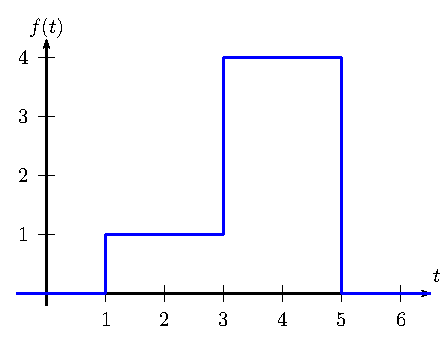
\includegraphics{cap_dirac_conv/pics/figura_16}\end{center}
\caption{\label{circ_3}}
\end{figure} 
\end{Exercise}
\begin{resp}
 $\displaystyle i(t) = e^{-t}\sen t - u(t-2)  e^{2-t} \sen (t-2)$
\end{resp}
\begin{Exercise}
Dada a equação do movimento de um oscilador harmônico simples (OHS)
\begin{equation}\label{ohs}
-k y(t) - \gamma y'(t) + f = my''(t),
\end{equation}
calcule a resposta $y(t)$ deste oscilador sujeito a forças externas $f$ do tipo dado abaixo. Considere $m=1$, $k=2$, $\gamma =3$, $y(0)=0$ e $y'(0)=0$.
\begin{itemize}
  \item[a)] $\displaystyle f(t) = \left\{
                                         \begin{array}{ll}
                                           1, & \hbox{ se } t\in [1,2] \\
                                           0, & \hbox{caso contrário}
                                         \end{array}
                                       \right.
  $
  \item[b)] $\displaystyle f(t) = \delta (t-1)$
\end{itemize}
\end{Exercise}
\begin{resp}
\begin{itemize}
\item[a)] $\displaystyle y(t) = \frac{1}{2}\big[ 1 -2 e^{1-t} + e^{2-2t} \big]u(t-1) - \frac{1}{2}\big[ 1 - 2 e^{2-t} + e^{4 - 2t} \big]$
  \item[b)] $\displaystyle y(t) = \big[ e^{1-t} - e^{2-2t}\big] u(t-1)$
\end{itemize}
\end{resp}
\begin{Exercise}
Considere um OHS não amortecido, isto é, $\gamma = 0$ na equação diferencial associada \eqref{ohs}. Suponha que este oscilador está sujeito a uma força externa dada por $f = F_0 \sen \left( \sqrt{k/m} t\right)$.
\begin{itemize}
  \item[a)] Use o método da transformada de Laplace para calcular as oscilações forçadas $y(t)$, sabendo que $y(0) = 0$ e $y'(0)=0$.
  \item[b)] Como se comporta o gráfico destas oscilações? Que fenômeno físico você identifica?
\end{itemize}
\end{Exercise}
\begin{resp}
 $\displaystyle \frac{F_0}{2k} \big[ \sen(\sqrt{k/m}t) - \sqrt{k/m}t \cos(\sqrt{k/m}t) \big] $
\end{resp}
\begin{Exercise}
Encontre por integração:
\begin{itemize}
  \item[a)] $1\ast 1$
  \item[b)] $t \ast e^t $
  \item[c)] $1\ast \cos(\omega t)$
  \item[d)] $e^{kt}\ast e^{-kt}$
\end{itemize}
\end{Exercise}
\begin{resp}
\begin{itemize}
  \item[a)] $\displaystyle t$
  \item[b)] $\displaystyle e^{t} - t - 1$
  \item[c)] $\displaystyle \frac{1}{\omega}\sen (\omega t)$
  \item[d)] $\displaystyle \frac{1}{2k} (e^{kt} - e^{-kt}) = \frac{1}{k}\senh (k t)$
\end{itemize}
\end{resp}
\begin{Exercise}
Achar a solução dos seguintes problemas de valor inicial:
\begin{itemize}
  \item[a)] $\displaystyle \left\{
                              \begin{array}{ll}
                                y'' + 2y'+2y = \delta(t-\pi)\\
                                y(0) = 1, \quad y'(0)=0
                              \end{array}
                            \right.
  $
  \item[b)] $\displaystyle \left\{
                              \begin{array}{ll}
                                y'' + 3y'+2y = \delta(t-5) - u(t-10)\\
                                y(0) = 0, \quad y'(0)=1/2
                                \end{array}
                            \right.
  $
  \item[c)] $\displaystyle \left\{
                              \begin{array}{ll}
                                y'' + y = \delta(t-2\pi)\\
                                y(0) = 0, \quad y'(0)=1
                              \end{array}
                            \right.
  $
\end{itemize}
\end{Exercise}
\begin{resp}
\begin{itemize}
  \item[a)] $\displaystyle y(t) = e^{-t} \sen t + e^\pi e^{-t} \sen (t-\pi) u (t-\pi)  + e^{-t} \cos t  = e^{-t} \sen t \big( 1 - e^\pi u (t-\pi) \big)  + e^{-t} \cos t$
  \item[b)] $\displaystyle y(t) = \frac{1}{2} ( e^{-t} - e^{-2t} ) +  ( e^{5-t} - e^{10-2t} )u(t-5) - \frac{1}{2} (1 - 2e^{10-t} + e^{20-2t} )u(t-10)$
  \item[c)] $\displaystyle y(t) = \sen t + \sen(t-2\pi) u(t-2\pi)$
\end{itemize}
\end{resp}
\begin{Exercise}
Justifique as seguintes propriedades da operação de convolução:
\begin{itemize}
  \item[a)] $f\ast g = g \ast f$
  \item[b)] $(f\ast g)\ast h = f \ast (g \ast h)$
  \item[c)] $f\ast (g + h) = f\ast g + f\ast h$
  \item[d)] $(\delta\ast f)(t) = f(t)$
\end{itemize}
{\it [Dica: cuidado para não confundir as variáveis de integração que aparecerão no item (b).}
\end{Exercise}
\begin{resp}
\begin{itemize}
  \item[a)] 
  \begin{eqnarray*}
   f\ast g&=&\int_0^t f(\tau)g(t-\tau)d\tau\\
   &=&-\int_t^0 f(t-u)g(u)du\\
   &=&\int_0^t g(u)f(t-u)du\\
   &=&g\ast f
  \end{eqnarray*}
  \item[b)] 
    \begin{eqnarray*}
   (f\ast g)\ast h&=& \int_0^t \left(\int_0^\tau f(u) g(\tau-u) du \right) h(t-\tau) d\tau \\
   &=& \int_0^t \int_0^\tau f(u) g(\tau-u) h(t-\tau) du d\tau \\
   &=& \int_0^t \int_u^t f(u) g(\tau-u) h(t-\tau)  d\tau du \\
   &=& \int_0^t f(u) \int_u^t g(\tau-u) h(t-\tau)  d\tau du \\
   &=& \int_0^t f(u) \int_0^{t-u} g(v) h(t-u-v)  dv du \\
   &=& \int_0^t f(u) \left[(g\ast h)(t-u)\right]  du \\
   &=&f \ast (g \ast h)
  \end{eqnarray*}
  onde se fez a mudança $v=\tau-u$, $dv=d\tau$.
\end{itemize}
\end{resp}
\begin{Exercise}
A equação do movimento de um OHS não amortecido sujeito a oscilações forçadas pode ser escrita como
$$
y''(t) + \omega^2 y(t) = r(t), \quad \hbox{ onde } \ \omega= \sqrt{\frac{k}{m}} \ \hbox{ e } \ r(t) = \frac{f(t)}{m}.
$$
\begin{itemize}
  \item[a)] Pelo método da transformada de Laplace, encontre $Y(s) = \mathcal{L} \left\{y(t)\right\}$.
  \item[b)] Com o auxílio do Teorema da Convolução, encontre $y(t)$ (em termos de $R = \mathcal{L}\{r\}$).
\end{itemize}
\end{Exercise}
\begin{resp}
\begin{itemize}
   \item[a)] $\displaystyle F(s) = \frac{sy(0)+y'(0)}{s^2 + w^2} + \frac{R(s)}{s^2 + w^2}$
  \item[b)] $\displaystyle y(t) = y(0) \cos (\omega t) + \frac{y'(0) \sen (\omega t)}{\omega} + \frac{\sen (\omega t)}{\omega} \ast r(t)$
\end{itemize}
\end{resp}
\begin{Exercise}
Use o Teorema da Convolução para calcular $$\mathcal{L}^{-1} \left( \frac{1}{(s+1)(s^2+1)} \right).$$
\end{Exercise}
\begin{resp}
 $\displaystyle \frac{1}{2} \big[ \sen t - \cos t + e^{-t} \big] $
\end{resp}
\begin{Exercise}
Use o Teorema da Convolução para resolver as seguintes equações integrais:
\begin{itemize}
  \item[a)] $\displaystyle y(t) = 1 + \int_0^t y(\tau) \ d\tau$
  \item[b)] $\displaystyle y(t) = 1 - \int_0^t y(\tau) (t-\tau) \ d\tau$
  \item[c)] $\displaystyle y(t) = te^{t} -2 e^t \int_0^t e^{-\tau} y(\tau) \ d\tau$
  \item[d)] $\displaystyle y(t) = 1 - \senh t + \int_0^t (1+ \tau )y(t- \tau) \ d\tau$
\end{itemize}
\end{Exercise}
\begin{resp}
\begin{itemize}
  \item[a)] $\displaystyle y(t) = e^{t}$
  \item[b)] $\displaystyle y(t) = \cos t$
  \item[c)] $\displaystyle y(t) = \senh t$
  \item[d)] $\displaystyle y(t) = \cosh t$
\end{itemize}
\end{resp}
\begin{Exercise}
Encontre
\begin{itemize}
  \item[a)] $\displaystyle \mathcal{L} \big\{ t u(t-1) + t^2 \delta(t-1) \big\}$
  \item[b)] $\displaystyle \mathcal{L} \big\{ (\cos t) ( \ln t ) \delta(t-\pi) \big\}$
  \item[c)] $\displaystyle \mathcal{L}\left\{ \delta(t-1) e^t \right\}$
\end{itemize}
\end{Exercise}
\begin{resp}
\begin{itemize}
  \item[a)] $\displaystyle \frac{ e^{-s} (s^2 + s + 1) }{s^2}$
  \item[b)] $\displaystyle -e^{-\pi s} \ln \pi $
  \item[c)] $\displaystyle e^{1-s}$
  \end{itemize}
\end{resp}

\chapter{Funções especiais e equações com coeficientes variáveis}
Nesse capítulo discutiremos a transformada de Laplace envolvendo funções especiais, tais como função de Bessel, função Gama e funções Seno Integrado. Também, desenvolveremos ferramentas capaz de resolver alguns problemas de valor iniciais com coeficientes não constantes.
Para iniciar as discussões vamos demonstrar o item 6 da tabela \ref{tab_trans_Lap_1} no próximo exemplo.
\begin{ex}Vamos calcular a transformada de Laplace da funçao $t^{k-1}$, dada por:
$$
\mathcal{L}\{t^{k-1} \}=\int_0^\infty t^{k-1} e^{-st}dt.
$$
Fazemos a mudança de variável $x=st$ para obter:
\begin{eqnarray*}
 \mathcal{L}\{t^{k-1} \}&=&\int_0^\infty \frac{x^{k-1}}{s^{k-1}}e^{-x}\frac{dx}{s}\\
 &=&\frac{1}{s^k}\int_0^\infty x^{k-1}e^{-x} dx.
 \end{eqnarray*}
A função que aparece acima é a multiplicação de $\frac{1}{s^k}$ por uma que não depende de $s$, chamada de função Gama e denotada por $\Gamma(k)$. Portanto, demonstramos o item (6) da tabela \ref{tab_trans_Lap_1}:
$$
\mathcal{L}\{t^{k-1} \}=\frac{\Gamma(k)}{s^k},\qquad k>0,
$$
onde
$$
\Gamma(k)=\int_0^\infty e^{-x}x^{k-1}dx.
$$
\end{ex}
Observe que o item 3 da tabela é
$$
\mathcal{L}\{t^{n-1}\}=\frac{(n-1)!}{s^n}, \qquad n\in \mathbb{N}.
$$
Isso nos indica que, para que os itens 3 e 6 sejam consistentes, $\Gamma(n+1)=n!$ se $n\in\mathbb{N}$. De fato, primeiro observe que, se $k=(n+1)\in\mathbb{N}$, temos:
$$
\Gamma(n+1)=\int_0^\infty e^{-x}x^{n}dx=\left[-e^{-x}x^{n}\right]_0^\infty-\int_0^\infty (-e^{-x})nx^{n-1}dx=n\int_0^\infty e^{-x}x^{n-1}dx=n\Gamma(n).
$$
Como 
$$
\Gamma(1)=\int_0^\infty e^{-x}dx=\left[-e^{-x}\right]_0^\infty=1,
$$
temos
$$
\Gamma(2)=1,\qquad \Gamma(3)=2\cdot 1=2!,\qquad \Gamma(4)=3\Gamma(3)=3\cdot 2!=3!,\cdots
$$
Logo, $\Gamma(n+1)=n!$ se $n\in\mathbb{N}$.
\begin{ex} Os itens 4 e 5 da tabela são casos particulares do item 6:
 $$
 \mathcal{L}\{t^{-\frac{1}{2}}\}=\frac{\Gamma\left(\frac{1}{2}\right)}{s^{\frac{1}{2}}}
 $$
e
 $$
 \mathcal{L}\{t^{\frac{1}{2}}\}=\frac{\Gamma\left(\frac{3}{2}\right)}{s^{\frac{3}{2}}}.
 $$
 Basta calcular os valores de $\Gamma\left(\frac{1}{2}\right)$ e $\Gamma\left(\frac{3}{2}\right)$ para completar a demonstração. Começamos com $\Gamma\left(\frac{1}{2}\right)$:
 $$
 \Gamma\left(\frac{1}{2}\right)=\int_0^\infty e^{-x}x^{-\frac{1}{2}}dx=\int_0^\infty \frac{e^{-x}}{\sqrt{x}}dx.
 $$
 Fazendo a mudança de variáveis $x=t^{2}$, obtemos $dx=2tdt$ e
$$\Gamma\left(\frac{1}{2}\right)=2\int_{0}^{\infty}e^{-t^2}dt
$$
Utilizando a técnica de Liouville, definimos:
$$
I=\int_{0}^{\infty}e^{-t^2}dt
$$
Logo
$$
I^2=\int_{0}^{\infty}e^{-x^2}dx\int_{0}^{\infty}e^{-y^2}dy=\int_{0}^{\infty}\int_{0}^{\infty}e^{-(x^2+y^2)}dx dy
$$
A última integral é uma integral dupla que pode ser calculada em coordenadas polares fazendo $r^2=x^2+y^2$ e $dxdy=rdrd\theta$:
$$
I^2=\int_{0}^{\frac{\pi}{2}}\int_{0}^{\infty}e^{-r^2}rdr d{\theta}=\frac{\pi}{2}\left[-\frac{e^{-r^2}}{2}\right]_0^\infty=\frac{\pi}{4}
$$
Assim,
$$
I^2=\frac{\pi}{4}\Rightarrow I=\frac{\sqrt{\pi}}{2}
$$
e
$$
\Gamma\left(\frac{1}{2}\right)=2\int_{0}^{\infty}e^{-t^2}dt=2I=\sqrt{\pi}.
$$
Agora, usando a propriedade da função Gama que $\Gamma(k+1)=k\Gamma(k)$, temos:
$$
\Gamma\left(\frac{3}{2}\right)=\frac{1}{2}\Gamma\left(\frac{1}{2}\right)=\frac{\sqrt{\pi}}{2}.
$$
Portanto, os itens 4 e 5 da tabela são válidos:
$$
 \mathcal{L}\{t^{-\frac{1}{2}}\}=\frac{\sqrt{\pi}}{\sqrt{s}}
$$
e
$$
 \mathcal{L}\{t^{\frac{1}{2}}\}=\frac{\sqrt{\pi}}{2s^{\frac{3}{2}}}.
$$
 \end{ex}
\begin{ex}Vamos calcular a transformada de Laplace da função $\ln(t)$ (item 38 da tabela \ref{tab_trans_Lap_2}). Com esse objetivo, usamos a transformada de Laplace de $t^k$ dada no item 6 da tabela \ref{tab_trans_Lap_2}:
$$
\int_0^\infty t^ke^{-st}dt=\frac{\Gamma(k+1)}{s^{k+1}}.
$$
Agora, como o integrando do lado esquerdo é uma função contínua e tem derivada parcial com respeito a $k$ contínua podemos diferenciar ambos os lados com respeito ao parâmetro $k$ usando a regra de Leibniz
\begin{eqnarray*}
\frac{d}{dk}\left(\int_0^\infty t^ke^{-st}dt\right)&=&\frac{d}{dk}\left(\frac{\Gamma(k+1)}{s^{k+1}}\right)\\
&\Downarrow&\\
\int_0^\infty t^k \ln(t) e^{-st}dt&=&\frac{s^{k+1}\Gamma'(k+1)-\Gamma(k+1)s^{k+1}\ln(s)}{s^{2(k+1)}}
\end{eqnarray*}
Agora, fazemos $k\to 0$ para obter
$$
\int_0^\infty \ln(t) e^{-st}dt=\frac{s^{1}\Gamma'(1)-\Gamma(1)s^{1}\ln(s)}{s^{2}},
$$
ou seja,
$$
\int_0^\infty \ln(t) e^{-st}dt=\frac{\Gamma'(1)-\ln(s)}{s},
$$
já que $\Gamma(1)=1$. Do lado esquerdo aparece a transformada da função $\ln(t)$ e do lado direito $\Gamma'(1)$. Então calculamos
$$
\Gamma'(k)=\int_0^\infty x^{k-1}\ln(x) e^{-x}dx
$$
e
$$
\Gamma'(1)=\int_0^\infty \ln(x) e^{-x} dx=\gamma=0.57721566490153286060651209008240243104215933593992 ...
$$
Essa constante $\gamma$ é chamada de constante de Euler - Mascheroni. Finalmente, concluímos
$$
\mathcal{L}\{\ln(t)\}=\frac{\gamma-\ln(s)}{s}
$$
\end{ex}
\section{Transformada de Laplace de funções periódicas}
Nesta seção apresentaremos uma propriedade da transformada de Laplace de funções periódicas e calcularemos algumas delas.
\begin{prop}{\label{prop_fun_per}}Seja $f(t)$ uma função contínua por partes e periódica de período $T$. Então sua transformada de Laplace é da forma
$$
\mathcal{L}\{f(t)\}=\frac{1}{1-e^{-sT}}\int_0^Tf(t)e^{-st}dt.
$$
\end{prop}
\begin{proof}Aplicamos a definição e separamos a integral nos períodos da função $f(t)$ para obter:
\begin{eqnarray*}
 \mathcal{L}\{f(t)\}&=&\int_0^\infty f(t)e^{-st}dt \\
 &=&\int_0^T f(t)e^{-st}dt+\int_T^{2T} f(t)e^{-st}dt+\int_{3T}^{4T} f(t)e^{-st}dt+\cdots\\
 &=&\sum_{n=0}^\infty \int_{nT}^{(n+1)T} f(t)e^{-st}dt.
\end{eqnarray*}
Fazemos a mudança de variável $\tau=t-nT$ e obtemos
 \begin{eqnarray*}
 \mathcal{L}\{f(t)\}&=&\sum_{n=0}^\infty \int_{0}^{T} f(\tau+nT)e^{-s(\tau+nT)}d\tau\\
 &=&\sum_{n=0}^\infty e^{-snT} \int_{0}^{T} f(\tau+nT)e^{-s\tau}d\tau.
 \end{eqnarray*}
 Usando o fato que a função é periódica, ou seja, $f(\tau)=f(\tau+nT)$, temos:
 \begin{eqnarray*}
  \mathcal{L}\{f(t)\}&=&\sum_{n=0}^\infty e^{-snT} \int_{0}^{T} f(\tau)e^{-s\tau}d\tau\\
 &=&\int_{0}^{T} f(\tau)e^{-s\tau}d\tau\left[\sum_{n=0}^\infty \left(e^{-sT}\right)^n \right]\\
 &=&\int_{0}^{T} f(\tau)e^{-s\tau}d\tau\left[\frac{1}{1-e^{-sT}} \right]\\
 &=&\frac{1}{1-e^{-sT}}\int_{0}^{T} f(\tau)e^{-s\tau}d\tau,
\end{eqnarray*}
onde usamos a soma de uma série geométrica de razão $e^{-sT}$.
 \end{proof}
\begin{ex}Observe o cálculo da transformada da função $f(t)=\cos(wt)$ sabendo que
$$
\int \cos(wt)e^{-st}dt=\frac{e^{-st}\left(w\sen(wt)-s\cos(wt)\right)}{s^2+w^2}+\ \!\hbox{Constante}
$$
e usando a propriedade \ref{prop_fun_per}:
\begin{eqnarray*} 
\mathcal{L}\{\cos(wt)\}&=&\frac{1}{1-e^{-s\frac{2\pi }{w}}}\int_0^{\frac{2\pi }{w}}\cos(wt)e^{-st}dt\\
&=&\frac{1}{1-e^{-s\frac{2\pi }{w}}}\left[\frac{e^{-st}\left(w\sen(wt)-s\cos(wt)\right)}{s^2+w^2}\right]_0^{\frac{2\pi }{w}}\\
&=&\frac{1}{1-e^{-s\frac{2\pi }{w}}}\frac{s-se^{-s\frac{2\pi }{w}}}{s^2+w^2}\\
&=&\frac{s}{s^2+w^2}.
\end{eqnarray*}
\end{ex}
\begin{ex}{\label{ex_onda_quadrada}}A função $f(t)$ apresentada no gráfico da figura \ref{fig_onda_quadrada} é chamada de {\bf onda quadrada} de período $2a$.
 \begin{figure}[!ht]
\begin{center}

\includegraphics{cap_especiais_coef_var/pics/figura_1}\end{center}
\caption{\label{fig_onda_quadrada}}
\end{figure}
Calculamos a transformada de Laplace usando a propriedade \ref{prop_fun_per} colocando $T=2a$
\begin{eqnarray*}
\mathcal{L}\{f(t)\}&=& \frac{1}{1-e^{-2sa}}\int_0^{2a}f(t)e^{-st}dt\\
&=& \frac{1}{1-e^{-2sa}}\left(\int_0^{a}e^{-st}dt-\int_a^{2a}e^{-st}dt\right)\\
&=& \frac{1}{1-e^{-2sa}}\left(\frac{1-2e^{-as}+e^{-2as}}{s}\right)\\
&=& \frac{1}{(1-e^{-sa})(1+e^{-sa})}\left(\frac{(1-e^{-as})^2}{s}\right)\\
&=&\frac{1}{s} \frac{1-e^{-as}}{1+e^{-sa}}.\\
\end{eqnarray*}
Multiplicando por $e^{\frac{as}{2}}$, podemos escrever a expressão em termos de funções hiperbólicas:
\begin{eqnarray*}
\mathcal{L}\{f(t)\}&=&\frac{1}{s} \frac{e^{\frac{as}{2}}-e^{-\frac{as}{2}}}{e^{\frac{as}{2}}+e^{-\frac{as}{2}})}\\
&=&\frac{1}{s} \frac{\senh\left(\frac{as}{2}\right)}{\cosh\left(\frac{as}{2}\right)}\\
&=&\frac{1}{s} \tanh\left(\frac{as}{2}\right).
\end{eqnarray*}
\end{ex}
\begin{ex}A função $g(t)$ apresentada no gráficoda figura \ref{fig_onda_triangular} é chamada de {\bf onda triangular} de perído $2a$.
 \begin{figure}[!ht]
\begin{center}

\includegraphics{cap_especiais_coef_var/pics/figura_2}\end{center}
\caption{\label{fig_onda_triangular}}
\end{figure}
Para calcular a transformada de Laplace, observe que:
\begin{itemize}
 \item[a)] A função $g(t)$ representada na figura \ref{fig_onda_triangular} tem como derivada uma onda quadrada. De fato, no intervalo $[0,a]$, a derivada é $\frac{1}{a}$ e no intervalo $[a,2a]$ a derivada é $-\frac{1}{a}$. Esse padrão se repete periodicamente. Logo, a derivada da onda triangular é a onda quadrada multiplicada por $\frac{1}{a}$.
 \item[b)] A propriedade \ref{prop_der} nos dá
 $$
 \mathcal{L}\{g(t)\}=\frac{1}{s}\mathcal{L}\{g'(t)\}+\frac{1}{s}g(0).
 $$
\end{itemize}
Logo,
\begin{eqnarray*}
\mathcal{L}\{\hbox{onda triangular}\}&=&\frac{1}{as}\mathcal{L}\{\hbox{onda quadrada}\}+\frac{1}{s}\hbox{(onda triangular na origem)},
\end{eqnarray*}
e, portanto, usando o fato que a onda triangular vale zero na origem e o resultado do exemplo \ref{ex_onda_quadrada}, temos
\begin{eqnarray*}
\mathcal{L}\{g(t)\}&=&\frac{1}{as}\frac{1}{s} \tanh\left(\frac{as}{2}\right)\\
&=&\frac{1}{as^2} \tanh\left(\frac{as}{2}\right).
\end{eqnarray*}
\end{ex}
\begin{ex} A função $h(t)$ dada por
$$
h(t)=\left\{\begin{array}{ll}\sen(wt),&0<t<\frac{\pi}{w}\\0,& \frac{\pi}{w}<t<\frac{2\pi}{w}, \end{array}\right.,
$$
$h\left(t+\frac{2\pi}{w}\right)=h(t)$, é chamada de {\bf retificador de meia onda} de período $\frac{2\pi}{w}$. A figura \ref{fig_ret_meia_onda} apresenta o gráfico da função $h(t)$.
 \begin{figure}[!ht]
\begin{center}

\includegraphics{cap_especiais_coef_var/pics/figura_3}\end{center}
\caption{\label{fig_ret_meia_onda}}
\end{figure}
Calculamos a transformada de Laplace usando a propriedade \ref{prop_fun_per} com $T=\frac{2\pi}{w}$
\begin{eqnarray*}
\mathcal{L}\{f(t)\}&=& \frac{1}{1-e^{-s\frac{2\pi}{w}}}\int_0^{\frac{2\pi}{w}}f(t)e^{-st}dt\\
&=& \frac{1}{1-e^{-s\frac{2\pi}{w}}} \int_0^{\frac{\pi}{w}}\sen(wt)e^{-st}dt\\
&=& \frac{1}{1-e^{-s\frac{2\pi}{w}}} \left[-\frac{e^{-st}\left(\sen(wt)+w\cos(wt)\right)}{s^2+w^2}\right]_0^{\frac{\pi}{w}}\\
&=& \frac{1}{(1-e^{-\frac{s\pi}{w}})(1+e^{-\frac{s\pi}{w}})} \frac{w(1+e^{-\frac{s\pi}{w}})}{s^2+w^2}\\
&=& \frac{1}{1-e^{-\frac{s\pi}{w}}} \frac{w}{s^2+w^2}
\end{eqnarray*}
\end{ex}
\begin{ex} A função $p(t)$ dada por
$$
p(t)=|\sen(wt)|
$$
é chamada de {\bf retificador de onda completa} de período $\frac{\pi}{w}$. A figura \ref{fig_ret_onda_completa} apresenta o gráfico da função $p(t)$.
 \begin{figure}[!ht]
\begin{center}

\includegraphics{cap_especiais_coef_var/pics/figura_4}\end{center}
\caption{\label{fig_ret_onda_completa}}
\end{figure}
Calculamos a transformada de Laplace usando a propriedade \ref{prop_fun_per} com $T=\frac{\pi}{w}$
\begin{eqnarray*}
\mathcal{L}\{p(t)\}&=& \frac{1}{1-e^{-s\frac{\pi}{w}}}\int_0^{\frac{\pi}{w}}\sen(wt)e^{-st}dt\\
&=& \frac{1}{1-e^{-s\frac{\pi}{w}}} \left[-\frac{e^{-st}\left(\sen(wt)+w\cos(wt)\right)}{s^2+w^2}\right]_0^{\frac{\pi}{w}}\\
&=& \frac{1}{1-e^{-\frac{s\pi}{w}}} \frac{w(1+e^{-\frac{s\pi}{w}})}{s^2+w^2}\\
&=&  \frac{w}{s^2+w^2}\frac{e^{\frac{s\pi}{2w}}+e^{-\frac{s\pi}{2w}}}{e^{\frac{s\pi}{2w}}-e^{-\frac{s\pi}{2w}}}\\
&=&  \frac{w}{s^2+w^2}\coth\left( \frac{\pi s}{2w}\right)
\end{eqnarray*}
\end{ex}
\begin{ex} A função $q(t)$ dada por
$$
\left\{\begin{array}{ll}q(t)=\frac{t}{a},&0\leq t<a\\ q\left(t+a\right)=q(t), & \end{array}\right.
$$
é chamada de {\bf onda dente de serra} de período $T=a$. A figura \ref{fig_dente_de_serra} apresenta o gráfico da função $q(t)$.
 \begin{figure}[!ht]
\begin{center}

\includegraphics{cap_especiais_coef_var/pics/figura_5}\end{center}
\caption{\label{fig_dente_de_serra}}
\end{figure}
Calculamos a transformada de Laplace usando a propriedade \ref{prop_fun_per} com $T=a$:
\begin{eqnarray*}
\mathcal{L}\{q(t)\}&=& \frac{1}{1-e^{-sa}} \int_0^{a} \frac{t}{a} e^{-st}dt\\
&=&\frac{1}{1-e^{-sa}}\frac{1}{a}\left[ -\frac{e^{-s t} (1+s t)}{s^2}\right]_0^a\\
&=&\frac{1}{1-e^{-sa}}\frac{1-e^{-sa}(1+as)}{s^2a} \\
&=&\frac{1}{1-e^{-sa}}\left(\frac{1-e^{-sa}-e^{-sa} as)}{s^2a} \right)\\
&=&\frac{1}{as^2}-\frac{e^{-sa} }{s\left(1-e^{-sa}\right)}.
\end{eqnarray*}
\end{ex}
\section{Séries de potências}
\subsection{Transformada de Laplace inversa de funções envolvendo expansão em séries de potências}
Em algumas situações, é conveniente expandir em séries de potência um termo de uma função para calcular sua transformada inversa. Vejamos alguns exemplos.
\begin{ex} Vamos calcular a transformada inversa da função $F(s)=\frac{1}{(s+1)(1-e^{-s})}$, usando o fato que
$$\frac{1}{1-e^{-s}}=1+e^{-s}+e^{-2s}+e^{-3s}+\cdots.$$
E, portanto, temos:
 $$ F(s)= \frac{1}{s+1}\left[1+e^{-s}+e^{-2s}+e^{-3s}+\cdots \right]
 $$
 Como, pelo item 7 da tabela de transformadas $\mathcal{L}^{-1}\left\{\frac{1}{s+1}\right\}=e^{-t}.$
Aplicando a propriedade do deslocamento no eixo $t$, temos:
 $$ f(t)= e^{-t}+ u(t-1) e^{-(t-1)}+ u(t-2) e^{-(t-2)}+ u(t-3) e^{-(t-3)}+\cdots.
 $$
O gráfico desta função é apresentado na figura \ref{fig_exp_iterada}.
 \begin{figure}[!ht]
\begin{center}

\includegraphics{cap_especiais_coef_var/pics/figura_6}\end{center}
\caption{\label{fig_exp_iterada}}
\end{figure}
\end{ex}
\begin{ex} Vamos calcular a transformada inversa da função $F(s)=\frac{e^{-s}}{s^2}\frac{\left(1-e^{-s}\right)^2}{1-e^{-3s}}$, usando o fato que
$$\frac{1}{1-e^{-3s}}=1+e^{-3s}+e^{-6s}+e^{-9s}+\cdots.$$
Agora observamos que se $g(t)=\mathcal{L}^{-1}\left\{\frac{e^{-s}{\left(1-e^{-s}\right)^2} }{s^2} \right\}$, então:
\begin{eqnarray*}
 g(t)&=&\mathcal{L}^{-1}\left\{\frac{e^{-s}{\left(1-e^{-s}\right)^2} }{s^2} \right\}=\mathcal{L}^{-1}\left\{\frac{e^{-s}\left(1-2e^{-s}+e^{-2s}\right) }{s^2} \right\}\\
 &=&\mathcal{L}^{-1}\left\{\frac{e^{-s}-2e^{-2s}+e^{-3s}}{s^2} \right\} = u(t-1) (t-1) + u(t-2) (4-2t) + u(t-3) (2t-4)
\end{eqnarray*}
Desta forma, pela propriedade do deslocamento em $t$, podemos escrever
\begin{eqnarray*}
f(t)&=&g(t)+u(t-3)g(t-3)+u(t-6)g(t-6)+u(t-9)g(t-9)+\cdots\\
&=&g(t)+g(t-3)+g(t-6)+g(t-9)+\cdots= \sum_{k=0}^\infty g(t-3k)
\end{eqnarray*}
o que implica
$$f(t)= \sum_{k=0}^\infty g(t-3k)=\sum_{k=0}^\infty\left[u(t-1-3k) (t-1-3k) + u(t-2-3k) (4-2t+6k) + u(t-3-3k) (2t-4-6k)\right]$$
O gráfico desta função é apresentado na figura \ref{fig_trian_periodica}.
 \begin{figure}[!ht]
\begin{center}

\includegraphics{cap_especiais_coef_var/pics/figura_7}\end{center}
\caption{\label{fig_trian_periodica}}
\end{figure}
\end{ex}
\subsection{Transformada de Laplace de funções envolvendo expansão em séries de potências}
Nesta seção, vamos calcular a transformada de Laplace usando a série de potências das funções e a linearidade da transformada.
\begin{ex}Vamos calcular $\mathcal{L}\{J_0(at)\}$ (item 31 da tabela \ref{tab_trans_Lap_2}), onde $J_0(at)$ é a função de Bessel de ordem zero dada por
$$
J_0(at)=1-\left(\frac{at}{2}\right)^2+\frac{1}{(2!)^2}\left(\frac{at}{2}\right)^4-\frac{1}{(3!)^2}\left(\frac{at}{2}\right)^6+\cdots.
$$
Aplicando o item 3 da tabela \ref{tab_trans_Lap_1}, temos:
\begin{eqnarray*}
\mathcal{L}\left\{J_0(at)\right\}&=&\mathcal{L}\left\{1\right\}-\left(\frac{a}{2}\right)^2\mathcal{L}\left\{t^2\right\}+\frac{1}{(2!)^2}\left(\frac{a}{2}\right)^4\mathcal{L}\left\{t^4\right\}-\frac{1}{(3!)^2}\left(\frac{a}{2}\right)^6\mathcal{L}\left\{t^6\right\}+\cdots\\
&=&\frac{1}{s}-\left(\frac{a}{2}\right)^2\frac{2!}{s^3}+\frac{1}{(2!)^2}\left(\frac{a}{2}\right)^4\frac{4!}{s^5}-\frac{1}{(3!)^2}\left(\frac{a}{2}\right)^6\frac{6!}{s^7}+\cdots\\
&=&\frac{1}{s}\left[1-\frac{1}{2}\left(\frac{a}{s}\right)^2+\frac{1}{2}\cdot \frac{3}{2}\cdot \frac{1}{2!}\left(\frac{a}{s}\right)^4-\frac{1}{2}\cdot\frac{3}{2}\cdot \frac{5}{2}\cdot\frac{1}{3!} \left(\frac{a}{s}\right)^6+\cdots\right]
\end{eqnarray*}
A série acima está apresentada no item 10 da tabela \ref{series_de_potencias}, onde usamos $m=-\frac{1}{2}$ e $x=\left(\frac{a}{s}\right)^2$. Logo,
\begin{eqnarray*}
\mathcal{L}\left\{J_0(at)\right\}&=&\frac{1}{s}\left(1+\left(\frac{a}{s}\right)^2\right)^{-\frac{1}{2}}
\end{eqnarray*}
\end{ex}
\begin{ex}Novamente usamos séries de potências para calcular $\mathcal{L}\{J_0(2\sqrt{kt})\}$, $k>0$ (item 34 da tabela \ref{tab_trans_Lap_2}). Aplicando o item 3 da tabela \ref{tab_trans_Lap_1}, temos:
\begin{eqnarray*}
\mathcal{L}\left\{J_0(2\sqrt{kt})\right\}&=&\mathcal{L}\left\{1-\left(\frac{2\sqrt{kt}}{2}\right)^2+\frac{1}{(2!)^2}\left(\frac{2\sqrt{kt}}{2}\right)^4-\frac{1}{(3!)^2}\left(\frac{2\sqrt{kt}}{2}\right)^6+\cdots\right\}\\
&=&\mathcal{L}\left\{1\right\}-k\mathcal{L}\left\{t\right\}+\frac{k^2}{(2!)^2}\mathcal{L}\left\{t^2\right\}-\frac{k^3}{(3!)^2}\mathcal{L}\left\{t^3\right\}+\cdots\\
&=&\frac{1}{s}-\frac{k}{s^2}+\frac{k^2}{(2!)^2}\frac{2!}{s^3}-\frac{k^3}{(3!)^2}\frac{3!}{s^4}+\cdots\\
&=&\frac{1}{s}\left[1-\left(\frac{k}{s}\right)^1+\frac{1}{2!}\left(\frac{k}{s}\right)^2-\frac{1}{3!}\left(\frac{k}{s}\right)^3+\cdots\right]\\
&=&\frac{1}{s}\left[1+\left(-\frac{k}{s}\right)^1+\frac{1}{2!}\left(-\frac{k}{s}\right)^2+\frac{1}{3!}\left(-\frac{k}{s}\right)^3+\cdots\right]
\end{eqnarray*}
A série acima está apresentada no item 3 da tabela \ref{series_de_potencias}, onde usamos $x=-\frac{k}{s}$. Logo,
\begin{eqnarray*}
\mathcal{L}\left\{J_0(2\sqrt{kt})\right\}&=&\frac{1}{s}e^{-\frac{k}{s}}
\end{eqnarray*}
\end{ex}
\begin{exer}Use o método das séries de potência e as propriedades da função $\Gamma$ para mostrar que
$$
\mathcal{L}\left\{\frac{\cos(2\sqrt{t})}{\sqrt{t}}\right\}=\frac{\sqrt{\pi}}{\sqrt{s}}e^{-\frac{1}{s}}.
$$
\end{exer}
\section{A derivada da transformada de Laplace}
\begin{prop}{\label{prop_der_transf}}
Se $F(s)=\mathcal{L}\{f(t)\}$, então
\begin{equation}
\frac{d}{ds}F(s)=-\mathcal{L}\{tf(t)\}.
\end{equation} 
\end{prop}
\begin{proof}
Usando a definição de transformada de Laplace, temos
\begin{eqnarray*}
\frac{d}{ds}F(s)&=&\frac{d}{ds}\int_0^\infty f(t) e^{-st}dt\\
&=&\int_0^\infty f(t) \frac{d}{ds}\left(e^{-st}\right)dt\\
&=&\int_0^\infty f(t) (-t)e^{-st}dt\\
&=&-\int_0^\infty tf(t) e^{-st}dt\\
&=&-\mathcal{L}\{tf(t)\}.
\end{eqnarray*}
\end{proof}
\begin{ex}Para calcular $\mathcal{L}\{t\cos(wt)\}$, usamos a propriedade \ref{prop_der_transf}:
\begin{eqnarray*}
\mathcal{L}\{t\cos(wt)\}&=&-\frac{d}{ds}\mathcal{L}\{\cos(wt)\}\\
&=&-\frac{d}{ds}\left(\frac{s}{s^2+w^2}\right)\\
&=&-\frac{-s^2+w^2}{(s^2+w^2)^2}\\
&=&\frac{s^2-w^2}{(s^2+w^2)^2}\\
\end{eqnarray*}
\end{ex}
\begin{exer}Calcule $\mathcal{L}\{t^2\sen(wt)\}$ usando a propriedade \ref{prop_der_transf}.
\end{exer}
\section{Equações diferenciais com coeficientes não constantes}
A propriedade \ref{prop_der_transf} da derivada da transformada de Laplace tem uma aplicação importante na solução de equações diferenciais com coeficientes variáveis.
\begin{ex}Vamos resolver o seguinte problema de valor inicial
\begin{eqnarray*}
ty''(t)+y'(t)+9ty(t)&=&0\\
y(0)&=&5\\
y'(0)&=&0.
\end{eqnarray*}
Começamos aplicando a transformada de Laplace na equação diferencial
$$
\mathcal{L}\{ty''(t)\}+\mathcal{L}\{y'(t)\}+9\mathcal{L}\{ty(t)\}=0.
$$
Depois aplicamos a propriedade \ref{prop_der_transf}:
$$
-\frac{d}{ds}\mathcal{L}\{y''(t)\}+\mathcal{L}\{y'(t)\}-9\frac{d}{ds}\mathcal{L}\{y(t)\}=0.
$$
Em seguida aplicamos a propriedade \ref{prop_der} para obter a seguinte equação subsidiária
$$
-\frac{d}{ds}\left(s^2Y(s)-5s\right)+sY(s)-5-9\frac{d}{ds}Y(s)=0,
$$
onde usamos que $y(0)=5$, $y'(0)=0$ e $Y(s)=\mathcal{L}\{y(t)\}$. Agora resolvemos as derivadas e obtemos uma equação diferencial mais simples para $Y(s)$:
$$
-s^2Y'(s)-2sY(s)+sY(s)-9Y'(s)=0,
$$
ou seja,
$$
\frac{Y'(s)}{Y(s)}=-\frac{s}{s^2+9}.
$$
Logo,
$$
\ln(Y(s))=-\frac{1}{2}\ln(s^2+9)+C,
$$
onde $C$ é uma constante de integração. Então
$$
Y(s)=K(s^2+9)^{-\frac{1}{2}}=\frac{K}{\sqrt{s^2+9}},
$$
onde $K=e^{C}$. Pelo item 31 da tabela \ref{tab_trans_Lap_1}, temos
$$
y(t)=KJ_0(3t).
$$
Como $J_0(0)=1$, usamos que $y(0)=5$ para obter $K=5$. Portanto,
$$
y(t)=5J_0(3t).
$$
Observe que a solução satisfaz $y'(0)=0$, porém essa condição não é necessária. De fato, existe uma solução linearmente independente dessa, que não possui transformada de Laplace, pode ser encontrada pelo método das séries de potência.
\end{ex}
\begin{ex}Vamos resolver a equação de Laguerre dada por
$$
ty''(t)+(1-t)y'(t)+2y(t)=0,
$$
com as condições iniciais $y(0)=1$ e $y'(0)=-2$. Primeiro aplicamos a transformada de Laplace nessa equação:
$$
\mathcal{L}\{ty''(t)\}+\mathcal{L}\{y'(t)\}-\mathcal{L}\{ty'(t)\}+2\mathcal{L}\{y(t)\}=0.
$$
Depois usamos a propriedade \ref{prop_der_transf}:
$$
-\frac{d}{ds}\mathcal{L}\{y''(t)\}+\mathcal{L}\{y'(t)\}+\frac{d}{ds}\mathcal{L}\{y'(t)\}+2\mathcal{L}\{y(t)\}=0.
$$
Continuamos usando a propriedade \ref{prop_der} para obter:
$$
-\frac{d}{ds}\left(s^2Y(s)-sy(0)-y'(0)\right)+sY(s)-y(0)+\frac{d}{ds}\left(sY(s)-y(0)\right)+2Y(s)=0,
$$
onde $Y(s)=\mathcal{L}\{y(t)\}$. Aplicando as derivadas chegamos na seguinte equação diferencial para $Y(s)$:
$$
-s^2Y'(s)-2sY(s)+y(0)+sY'(s)+Y(s)+sY(s)-y(0)+2Y(s)=0.
$$
ou seja,
$$
Y'(s)\left(-s^2+s\right)+Y(s)\left(-s+3\right)=0.
$$
Logo,
$$
\frac{Y'(s)}{Y(s)}=-\frac{3-s}{s(1-s)}.
$$
Usamos o método de separação de variáveis para resolver a equação diferencial, temos:
$$
\ln(Y(s))=-\int \frac{3-s}{s(1-s)} ds +C
$$
onde $C$ é uma constante de integração. A antiderivada do lado direito pode ser obtida pelo método de frações parciais:
\begin{eqnarray*}
\frac{-3+s}{s(1-s)}=-\frac{3}{s}-\frac{2}{1-s}.
\end{eqnarray*}
Isso nos dá
$$
\ln(Y(s))=-3\ln(s)+2\ln|1-s|+C=\ln\left(\frac{(1-s)^2}{s^3} \right)+C
$$
ou
$$
Y(s)=K\frac{(1-s)^2}{s^3}=\frac{K}{s^3}-\frac{2K}{s^2}+\frac{K}{s}
$$
onde $K=e^C$. A transformada inversa fornece uma expressão para $y(t)$:
$$
y(t)=K\left(\frac{t^2}{2}-2t+1\right).
$$
Usando o fato que $y(0)=1$, temos $K=1$ e
$$
y(t)=\frac{t^2}{2}-2t+1.
$$
Observe que, apesar da condição para a derivada ser satisfeita, isto é,
$$
y'(0)=0-2=-2,
$$
não usamos-a para calcular a solução. De fato, o problema possui um singularidade na origem que não é percebida pela transformada de Laplace. A solução linearmente independente dessa, que não possui transformada de Laplace, pode ser encontrada pelo método das séries de potência.
\end{ex}
\section{Propriedade da integral da transformada de Laplace}
\begin{prop}{\label{prop_int_transf}}Se $F(s)$ é a transformada de Laplace de $f(t)$ e a função
e o limite
$$
\lim_{t\to 0^+}\int_{t}^1\frac{f(\tau)}{\tau}d\tau
$$
existe, então
\begin{equation}
\int_s^\infty F(v)dv =\mathcal{L}\left\{\frac{f(t)}{t}\right\}.
\end{equation}
 \end{prop}
\begin{proof} Usamos a definição de transformada de Laplace para escrever
\begin{eqnarray*}
\int_s^\infty F(v)dv&=&\int_s^\infty\left(\int_0^\infty f(t)e^{-vt}dt\right)dv\\
&=&\int_0^\infty f(t)\left(\int_s^\infty e^{-vt} dv \right)dt\\
&=&\int_0^\infty f(t)\left[\frac{ e^{-vt}}{-t} \right]_s^\infty dt\\
&=&\int_0^\infty \frac{f(t)}{t} e^{-st}  dt\\
&=&\mathcal{L}\left\{ \frac{f(t)}{t} \right\}.
\end{eqnarray*}
Observe que a existência do limite $\lim_{t\to 0^+}\int_{t}^1\frac{f(\tau)}{\tau}d\tau$ é fundamental para a existência da Transformada de Laplace e para os procedimentos analíticos acima.
\end{proof}
\begin{ex}Vamos mostrar o item 29 da tabela \ref{tab_trans_Lap_2}:
$$
\mathcal{L}\left\{\frac{1}{2\sqrt{\pi t^3}}\left(e^{bt}-e^{at}\right)\right\}=\sqrt{s-a}-\sqrt{s-b}.
$$
Para isso vamos usar o item 4, a saber,
\begin{equation}{\label{eq_item_4}}
\mathcal{L}\left\{\frac{1}{\sqrt{\pi t}}\right\}=\frac{1}{\sqrt{s}}.
\end{equation}
Aplicamos a propriedade \ref{prop_trans_s} da translação no eixo $s$ na equação (\ref{eq_item_4}) para obter:
\begin{equation*}
\mathcal{L}\left\{\frac{1}{\sqrt{\pi t}}e^{at}\right\}=\frac{1}{\sqrt{s-a}}.
\end{equation*}
Finalmente, usando a propriedade \ref{prop_int_transf} da integral da transformada, obtemos:
\begin{eqnarray*}
\mathcal{L}\left\{\frac{1}{2\sqrt{\pi t^3}}\left(e^{bt}-e^{at}\right)\right\}&=&\frac{1}{2}\mathcal{L}\left\{\frac{1}{t}\left(\frac{1}{\sqrt{\pi t}}e^{bt}-\frac{1}{\sqrt{\pi t}}e^{at}\right)\right\}\\
&=&\frac{1}{2}\int_s^\infty\left(   \frac{1}{\sqrt{v-b}}-  \frac{1}{\sqrt{v-a}}\right)dv\\
&=&\frac{1}{2}\int_s^\infty  \left( \left(v-b\right)^{-\frac{1}{2}}-  \left(v-a\right)^{-\frac{1}{2}}\right)dv\\
&=&\left. -\left(v-b\right)^{\frac{1}{2}}+ \left(v-a\right)^{\frac{1}{2}}\right|_s^\infty\\
&=&\sqrt{s-a}-\sqrt{s-b}.
\end{eqnarray*}
Observe que aqui usamos o seguinte limite no infinito
\begin{eqnarray*}
\lim_{v\to\infty}\left( \sqrt{v-b}- \sqrt{v-a}\right)&=&\lim_{v\to\infty}\frac{\left(\sqrt{v-b}- \sqrt{v-a}\right)\left(\sqrt{v-b}+ \sqrt{v-a}\right)}{\left(\sqrt{v-b}+ \sqrt{v-a}\right)}\\
&=&\lim_{v\to\infty}\frac{\left((v-b)- (v-a)\right)}{\left(\sqrt{v-b}+ \sqrt{v-a}\right)}\\
&=&\lim_{v\to\infty}\frac{\left(a-b\right)}{\left(\sqrt{v-b}+ \sqrt{v-a}\right)}\\
&=&0.
\end{eqnarray*}
\end{ex}
\begin{ex}Vamos mostrar o item 39 da tabela \ref{tab_trans_Lap_2}:
$$
\mathcal{L}\left\{\frac{1}{t}\left(e^{bt}-e^{at}\right)\right\}=\ln\left(\frac{s-a}{s-b}\right).
$$
Para isso vamos usar o item 7, a saber,
\begin{equation*}
\mathcal{L}\left\{e^{at}\right\}=\frac{1}{s-a}.
\end{equation*}
Usando a propriedade \ref{prop_int_transf} da integral da transformada, obtemos:
\begin{eqnarray*}
\mathcal{L}\left\{\frac{1}{t}\left(e^{bt}-e^{at}\right)\right\}&=&\int_s^\infty \left(\frac{1}{v-b}-\frac{1}{v-a}\right)dv\\
&=& \left.\left(\ln(v-b)-\ln(v-a)\right)\right|_s^\infty\\
&=& \left(\ln(s-a)-\ln(s-b)\right)\\
&=&\ln\left(\frac{s-a}{s-b}\right)
\end{eqnarray*}
Na penúltima igualdade usamos o seguinte limite no infinito:
\begin{eqnarray*}
\lim_{v\to\infty} \left(\ln(v-b)-\ln(v-a)\right)&=&\lim_{v\to\infty} \ln\left(\frac{v-b}{v-a}\right)\\
&=& \ln\left(\lim_{v\to\infty}\left(\frac{v-b}{v-a}\right)\right)\\
&=& \ln\left(1\right)\\
&=&0.
\end{eqnarray*}
Observe que a troca do limite com o logarítmo é possível visto que $\ln(x)$ é contínua para $x>0$.
\end{ex}
\begin{ex}Vamos mostrar o item 40 da tabela \ref{tab_trans_Lap_2}:
$$
\mathcal{L}\left\{\frac{2}{t}\left(1-\cos(wt)\right)\right\}=\ln\left(\frac{s^2+w^2}{s^2}\right).
$$
Para isso vamos usamos o fato que
\begin{equation*}
\mathcal{L}\left(1-\cos(wt)\right)=\frac{1}{s}-\frac{s}{s^2+w^2}.
\end{equation*}
Usando a propriedade \ref{prop_int_transf} da integral da transformada, obtemos:
\begin{eqnarray*}
\mathcal{L}\left\{\frac{2}{t}\left(1-\cos(wt)\right)\right\}&=&2\int_s^\infty \left(\frac{1}{v}-\frac{v}{v^2+w^2}\right)dv\\
&=& \left.2\left(\ln(v)-\frac{1}{2}\ln(v^2+w^2)\right)\right|_s^\infty\\
&=& \left.\left(2\ln(v)-\ln(v^2+w^2)\right)\right|_s^\infty\\
&=&\left.\ln\left(\frac{v^2}{v^2+w^2}\right)\right|_s^\infty\\
&=&-\ln\left(\frac{s^2}{s^2+w^2}\right)\\
&=&\ln\left(\frac{s^2+w^2}{s^2}\right)
\end{eqnarray*}
Na penúltima igualdade usamos o seguinte limite no infinito:
\begin{eqnarray*}
\lim_{v\to\infty} \ln\left(\frac{v^2}{v^2+w^2}\right)&=& \ln\left(\lim_{v\to\infty}\left(\frac{v^2}{v^2+w^2}\right)\right)\\
&=& \ln\left(1\right)\\
&=&0.
\end{eqnarray*}
Observe que a troca do limite com o logarítmo é possível visto que $\ln(x)$ é contínua para $x>0$.
\end{ex}
\begin{exer}Demonstre o item 41 da tabela usando os itens 1 e 16 juntamente com a propriedade \ref{prop_int_transf}.
\end{exer}
\begin{ex}{\label{ex_sint_t}}Vamos demonstrar o item 42 da tabela \ref{tab_trans_Lap_2}:
$$
\mathcal{L}\left\{\frac{1}{t}\sen(wt)\right\}=\arctan\left(\frac{w}{s}\right).
$$
Para isso vamos usamos o fato que
\begin{equation*}
\mathcal{L}\{\sen(wt)\}=\frac{w}{s^2+w^2}.
\end{equation*}
Usando a propriedade \ref{prop_int_transf} da integral da transformada, obtemos:
\begin{eqnarray*}
\mathcal{L}\left\{\frac{1}{t}\sen(wt)\right\}&=&\int_s^\infty \left(\frac{w}{v^2+w^2}\right)dv\\
&=& \left.\arctan\left(\frac{v}{w}\right)\right|_s^\infty\\
&=&\lim_{v\to\infty}\arctan\left(\frac{v}{w}\right)-\arctan\left(\frac{s}{w}\right)\\
&=&\frac{\pi}{2}-\arctan\left(\frac{s}{w}\right)\\
\end{eqnarray*}
Usando o fato que $\tan\left(\frac{\pi}{2}-\theta\right)=\cot(\theta)$, temos que
\begin{eqnarray*}
\mathcal{L}\left\{\frac{1}{t}\sen(wt)\right\}=\cot^{-1}\left(\frac{s}{w}\right).
\end{eqnarray*}
Também, se $\gamma=\cot^{-1}\left(\frac{s}{w}\right)$, então $\cot\gamma=\frac{s}{w}$. Logo, $\frac{1}{\tan\gamma}=\frac{s}{w}$ e, portanto, $\tan\gamma=\frac{w}{s}$. Assim, podemos escrever a transformada de Laplace da seguinte forma:
\begin{eqnarray*}
\mathcal{L}\left\{\frac{1}{t}\sen(wt)\right\}=\arctan\left(\frac{w}{s}\right)
\end{eqnarray*}
\end{ex}
\begin{ex}Vamos agora mostrar o item 43 da tabela \ref{tab_trans_Lap_2}:
$$
\mathcal{L}\left\{\hbox{Si}\ \!(t)\right\}=\frac{1}{s}\cot^{-1}(s),
$$
onde $\hbox{Si}\ \!(t)$ é função integral seno dada por:
$$
\hbox{Si}\ \!(t)=\int_0^t\frac{\sen(x)}{x}dx.
$$
Primeiro aplicamos a propriedade \ref{prop_trans_int} para obter
$$
\mathcal{L}\left\{\hbox{Si}\ \!(t)\right\}=\mathcal{L}\left\{\int_0^t\frac{\sen(x)}{x}dx\right\}=\frac{1}{s}\mathcal{L}\left\{\frac{\sen(t)}{t}\right\}.
$$
Em seguida usamos o resultado do exemplo \ref{ex_sint_t} (ou item 42 da tabela \ref{tab_trans_Lap_2}) e temos:
$$
\mathcal{L}\left\{\hbox{Si}\ \!(t)\right\}=\frac{1}{s}\arctan\left(\frac{1}{s}\right)=\frac{1}{s}\cot^{-1}\left(s\right).
$$
\end{ex}
\section{Propriedades do Valor Inicial e Final}
\begin{prop}(Propriedade do Valor Final) Se $F(s)$ é a transformada de Laplace de $f(t)$ e 
$$
\lim_{t\to\infty}f(t)=L,
$$
então
$$
\lim_{s\to 0^+} sF(s)=L.
$$
\end{prop}
\begin{proof}Usamos a definição de transformada de Laplace para escrever
\begin{eqnarray*}
sF(s)&=&s\int_0^\infty f(t)e^{-st}dt\\
&=&s\int_0^a f(t)e^{-st}dt+s\int_a^\infty f(t)e^{-st}dt.\\
\end{eqnarray*}
Observe que a primeira parcela do lado direito tende a zero independentemente do valor de $a$. Porém, para $a$ suficientemente grande, $f(t)$ se aproxima de $L$, pois $\displaystyle \lim_{t\to\infty}f(t)=L$, ou seja,
\begin{eqnarray*}
s\int_a^\infty f(t)e^{-st}dt &\approx &s\int_a^\infty L e^{-st}dt.\\
&\approx &s\frac{L}{-s}\left[ e^{-st}\right]_a^\infty=Le^{-as}
\end{eqnarray*}
Como $e^{-as}\to 1$ quando $s\to 0$, então
$$
\lim_{s\to 0^+} sF(s)=L.
$$ 
\end{proof}
\begin{prop}(Propriedade do Valor Inicial) Se $F(s)$ é a transformada de Laplace de uma função $f(t)$ de ordem exponencial $c$ e 
$$
\lim_{t\to 0^+}f(t)=L,
$$
então
$$
\lim_{s\to \infty} sF(s)=L.
$$
\end{prop}
\begin{proof}Usamos a definição de transformada de Laplace para escrever
\begin{eqnarray*}
sF(s)&=&s\int_0^\infty f(t)e^{-st}dt\\
&=&s\int_0^a f(t)e^{-st}dt+s\int_a^b f(t)e^{-st}dt+s\int_b^\infty f(t)e^{-st}dt.\\
\end{eqnarray*}
Observe que a segunda parcela do lado direito tende a zero quando $s\to \infty$ independentemente do valor de $a$ e $b$, pois o fato da função ser de ordem exponencial e contínua por partes implica em $f(t)$ limitada em $[a,b]$, ou seja, $|f(t)|<M$ e, portanto,
\begin{eqnarray*}
\left|s\int_a^b f(t)e^{-st}dt\right|&\leq & s\int_a^b |f(t)|e^{-st}dt\\
&\leq & Ms\int_a^b e^{-st}dt\\
&\leq & \left.Ms\frac{1}{-s} e^{-st}\right|_a^b=M(e^{-sa}-e^{-sb}).
\end{eqnarray*}
Também, a terceira parcela tende a zero se $b$ for suficientemente grande, pois existem $c$ e $M>0$ tal que $|f(t)|<Me^{ct}$ para $t>b$ e, portanto,
\begin{eqnarray*}
\left|s\int_b^\infty f(t)e^{-st}dt\right|&\leq & s\int_b^\infty |f(t)|e^{-st}dt\\
&\leq & s\int_b^\infty Me^{-(s-c)t}dt\\
&\leq & \left.Ms\frac{1}{c-s} e^{-(s-c)t}\right|_b^\infty=\frac{Ms}{s-c}(e^{-(s-c)b}).
\end{eqnarray*}
Porém, para $a$ suficientemente pequeno, $f(t)$ se aproxima de $L$, pois $\displaystyle \lim_{t\to 0}f(t)=L$, ou seja,
\begin{eqnarray*}
s\int_0^a f(t)e^{-st}dt &\approx &s\int_0^a L e^{-st}dt.\\
&\approx &s\frac{L}{-s}\left[ e^{-st}\right]_0^a=L\left(1-e^{-as}\right)
\end{eqnarray*}
Como $e^{-as}\to 0$ quando $s\to \infty$, então
$$
\lim_{s\to \infty} sF(s)=L.
$$ 
\end{proof}
\section{Exercícios}
\begin{Exercise}
 Demonstre o item (32) da tabela usando os itens (4) e (5) e a propriedade \ref{prop_trans_s} do deslocamento no eixo $s$. 
\end{Exercise}
\begin{Exercise}
Use a propriedade da derivada da transformada para calcular $\displaystyle \mathcal{L}\{ t \cos (\omega t) \}$. A partir desta, prove que $$ \mathcal{L}\{ \sen (\omega t) - \omega t \cos (\omega t) \} = \frac{2 \omega^3 }{(s^2 + \omega^2)^2}. $$
\end{Exercise}
\begin{Exercise}
Encontre a transformada inversa das funções abaixo utlizando o método que achar adequado.
\begin{itemize}
\item[a)] $\displaystyle F(s)= \frac{3s + 7}{s^2 - 2 s - 3}$.
\item[b)] $\displaystyle F(s)= \frac{1}{(s-2)^3}$.
\item[c)] $\displaystyle F(s)= \frac{3s + 1}{(s-1)(s^2 +1)}$.
\item[d)] $\displaystyle F(s)= \frac{s + 12}{s^2 +4s}$.
\item[e)] $\displaystyle F(s)= \frac{s -3}{s^2 -1}$.
\item[f)] $\displaystyle F(s)= \frac{3s}{s^2 +2s -8}$.
\item[g)] $\displaystyle F(s)= \frac{3s^2 -2s - 1}{(s-3)(s^2 +1)}$.
\item[h)] $\displaystyle F(s)= \frac{s + 1}{s^2 +4s +13}$.
\item[i)] $\displaystyle F(s)= \frac{s^2 + s -2}{(s +1)^3}$.
\item[j)] $\displaystyle F(s)= \frac{2s^3 +10s^2+8s+40}{s^2(s^2 +9)}$.
\item[k)] $\displaystyle F(s)= \frac{2s^2 -4}{(s+1)(s-2)(s-3)}$.
\item[l)] $\displaystyle F(s)= \frac{1}{(s^2+4)(s^2 +1)}$.
\end{itemize}
\end{Exercise}
\begin{resp}
\begin{itemize}
  \item[a)] $\displaystyle f(t) = 4e^{3t} - e^{-t}$
  \item[b)] $\displaystyle f(t) = \frac{1}{2} t^2 e^{2t}$
  \item[c)] $\displaystyle f(t) = 2e^{t} - 2 \cos t + \sen t$
  \item[d)] $\displaystyle f(t) = 3 -2 e^{-4t}$
  \item[e)] $\displaystyle f(t) = \cosh t - 3 \senh t$
  \item[f)] $\displaystyle f(t) = 2e^{-4t} + e^{2t}$
  \item[g)] $\displaystyle f(t) = 2e^{3t} + \cos t + \sen t$
  \item[h)] $\displaystyle f(t) = e^{-2t}\bigg[ \cos(3t) - \frac{1}{3} \sen (3t) \bigg]$
  \item[i)] $\displaystyle f(t) = e^{-t}(1-t-t^2)$
  \item[j)] $\displaystyle f(t) = 2\cos(3t) +\frac{10}{3} \sen(3t) +\frac{8}{9} \big[1-\cos(3t)\big] + \frac{40}{27} \big[3t - \sen(3t)\big]$
  \item[k)] $\displaystyle f(t) = -\frac{1}{6} e^{-t} -\frac{4}{3} e^{2t} + \frac{7}{2} e^{3t}$
  \item[l)] $\displaystyle f(t) = \frac{1}{3} \bigg[ \sen t - \frac{1}{2}\sen(2t) \bigg]$
\end{itemize}
\end{resp}
\begin{Exercise}
Use a tabela da transformada de Laplace para mostrar que:
\begin{itemize}
  \item[a)] $\displaystyle \mathcal{L} \big\{ t^{1/2}+ t^{-1/2} \big\} = \frac{\sqrt{\pi}(2s+1)}{2s^{3/2}}$
  \item[b)] $\displaystyle \mathcal{L} \bigg\{ \frac{e^{-2t}}{\sqrt{t}} \bigg\} = \sqrt{\frac{\pi}{s+2}}$
  \item[c)] $\displaystyle \mathcal{L} \bigg\{ \frac{\cos(2\sqrt{t}) }{\sqrt{t}} \bigg\} = e^{-1/s}\sqrt{\frac{\pi}{s}}$
\end{itemize}
\end{Exercise}
\begin{Exercise}
Use o método das séries de potências para mostrar que \[\mathcal{L} \{\sen \sqrt{t} \} =  \frac{\sqrt{\pi} e^{-1/4s}}{2s^{3/2}}.\]
\emph{Sugestão}: Use que \[\Gamma\bigg( n + \frac{3}{2} \bigg) = \frac{ (2n+1)!}{ n! 2^{2n+1}}\sqrt{\pi}.\]
\end{Exercise}
\begin{resp}
 \begin{eqnarray*}
f(t)&=&\sin\sqrt{t}= \sum_{n=0}^{\infty}(-1)^n\frac{t^{(2n+1)/2}}{(2n+1)!}\\
F(s)&=&\mathcal{L}\left\{f(t)\right\}=\sum_{n=0}^{\infty}\frac{(-1)^n}{{(2n+1)!}}\mathcal{L}\left\{{t^{(2n+1)/2}}\right\}\\
&=&\sum_{n=0}^{\infty}\frac{(-1)^n}{{(2n+1)!}}\mathcal{L}\left\{{t^{(2n+1)/2}}\right\}\\
&=&\sum_{n=0}^{\infty}\frac{(-1)^n}{{(2n+1)!}}\Gamma\left((2n+3)/2\right)\frac{1}{s^{(2n+3)/2}}\\
&=&\sum_{n=0}^{\infty}\frac{(-1)^n}{{(2n+1)!}}\frac{(2n+1)!}{n!}\frac{\sqrt{\pi}}{2^{2n+1}}\frac{1}{s^{(2n+3)/2}}\\
&=&\frac{\sqrt{\pi}}{2s^{3/2}}\sum_{n=0}^{\infty}{(-1)^n}\frac{1}{n!}\frac{1}{2^{2n}}\frac{1}{s^{n}}\\
&=&\frac{\sqrt{\pi}}{2s^{3/2}}\sum_{n=0}^{\infty}\frac{1}{n!}{\left(-\frac{1}{4s}\right)^{n}}\\
&=&\frac{\sqrt{\pi}}{2s^{3/2}}e^{-\frac{1}{4s}}
\end{eqnarray*}
Para mostrar a identidade $\Gamma\bigg( n + \frac{3}{2} \bigg) = \frac{ (2n+1)!}{ n! 2^{2n+1}}\sqrt{\pi}$ , usamos a relação de recorrência
$$\Gamma(x+1)=x\Gamma(x)$$
e o fato bem conhecido  de que
$$\Gamma(1/2)=\sqrt{\pi}$$
Para obter
\begin{eqnarray*}
\Gamma(3/2)&=&\Gamma(1+1/2)=\frac{1}{2}\Gamma(1/2)=\frac{\sqrt{\pi}}{2}\\
\Gamma(5/2)&=&\Gamma(1+3/2)=\frac{3}{2}\Gamma(3/2)=\frac{3\sqrt{\pi}}{2^2}\\
\Gamma(7/2)&=&\Gamma(1+5/2)=\frac{5}{2}\Gamma(5/2)=\frac{5 \cdot 3\sqrt{\pi}}{2^3}\\
\Gamma(9/2)&=&\Gamma(1+7/2)=\frac{7}{2}\Gamma(7/2)=\frac{7\cdot 5 \cdot 3\sqrt{\pi}}{2^4}\\
\end{eqnarray*}
E generalizando, temos:
\begin{eqnarray*}
\Gamma\left(\frac{2n+1}{2}\right)&=&\Gamma\left(1+\frac{2n-1}{2}\right)=\frac{2n-1}{2}\Gamma\left(\frac{2n-1}{2}\right)={(2n-1)(2n-3)\cdots 3}\frac{\sqrt{\pi}}{2^{n}}\\
&=&\frac{(2n-1)(2n-2)(2n-3)\cdots 3\cdot 2 \cdot 1}{(2n-2)(2n-4)\cdots 2}\frac{\sqrt{\pi}}{2^{n}}\\
&=&\frac{(2n-1)(2n-2)(2n-3)\cdots 3\cdot 2 \cdot 1}{2^{n-1}(n-1)(n-2)\cdots 1}\frac{\sqrt{\pi}}{2^{n}}\\
&=&\frac{(2n-1)!}{(n-1)!}\frac{\sqrt{\pi}}{2^{2n-1}}
\end{eqnarray*}
\end{resp}
\begin{Exercise}
Usando a derivada da transformada de Laplace, calcule:
\begin{itemize}
  \item[a)] $\displaystyle \mathcal{L} \{ t \senh (at) \}$
  \item[b)] $\displaystyle \mathcal{L} \{ t \cosh (at) \}$
\end{itemize}
\end{Exercise}
\begin{resp}
 \begin{itemize}
  \item[a)] $\displaystyle \frac{2as}{(s^2 - a^2)^2}$
  \item[b)] $\displaystyle \frac{s^2 + 9}{(s^2 - 9)^2}$
 \end{itemize}
\end{resp}
\begin{Exercise}
Resolva
\[
\left\{
  \begin{array}{ll}
    ty'' (t) + 2y'(t) +ty(t) = 0 \\
    y(0)=1, \quad y(\pi) = 0
  \end{array}
\right.
\] \emph{Sugestão}: Utilize que $\displaystyle \lim_{s\to + \infty} Y(s) = 0.$
\end{Exercise}
\begin{resp}
 $\displaystyle y(t) = \frac{\sen t}{t}$
\end{resp}
\begin{Exercise}
Utilize a integral da transformada de Laplace para demonstrar que:
\begin{itemize}
  \item[a)] $\displaystyle \mathcal{L}\bigg\{ \frac{\senh t}{t} \bigg\} = \frac{1}{2} \ln \bigg(\frac{s+1}{s-1}\bigg)$
  \item[b)] $\displaystyle \mathcal{L}\bigg\{ \frac{2}{t} \big( 1 - \cos (\omega t) \big) \bigg\} = \ln \bigg(\frac{s^2 + \omega^2}{s^2}\bigg)$
  \item[c)] $\displaystyle \mathcal{L}\bigg\{ \frac{2}{t} \big( 1 - \cosh (\omega t) \big) \bigg\} = \ln \bigg(\frac{s^2 - \omega^2}{s^2}\bigg)$
\end{itemize}
\end{Exercise}
\begin{resp}
 \begin{itemize}
  \item[a)] $\displaystyle \frac{ 3 - 3 e^{-2s} - 6s e^{-4s} }{s^2 (1 - e^{-4s})}$
  \item[b)] $\displaystyle \frac{  e^{2\pi(1-s)} -1 }{(1-s) (1 - e^{-2\pi s})}$
  \item[c)] $\displaystyle \frac{\omega}{s^2 + \omega^2} \coth \bigg(\frac{\pi s}{2 \omega^2} \bigg)$
 \end{itemize}
\end{resp}
\begin{Exercise}
Faça o gráfico de $f(t)$ e calcule $\mathcal{L}\big\{f(t)\big\}$.
\begin{itemize}
  \item[a)] $f$ periódica de período $p=4$ e $\displaystyle f(t) = \left\{
                                                                      \begin{array}{ll}
                                                                        3t, & \hbox{ se } t \in (0,2) \\
                                                                        6, & \hbox{ se } t \in (2,4)
                                                                      \end{array}
                                                                    \right.
$
  \item[b)] $f$ periódica de período $p=2\pi$ e $\displaystyle f(t) = e^t$, para $t \in (0,2\pi)$.
  \item[b)] $\displaystyle f(t) = |\sen (\omega t)|$.
\end{itemize}
\end{Exercise}
\begin{resp}
 \begin{itemize}
  \item[a)] $\displaystyle y(t) = 10 \cos (2t) + \frac{k}{8} \Big( 1 - \cos \big(2(t-a)\big) \Big)u(t-a) $
  \item[b)] $\displaystyle y(t) = 10 \cos (2t) + \frac{k}{4} \sen(2t)$
 \end{itemize}
\end{resp}
\begin{Exercise}
Para $k$ constante, encontre a solução de
\begin{itemize}
  \item[a)] $\displaystyle \left\{
                              \begin{array}{ll}
                                2y''(t) + 8 y(t) = k u(t-a) \\
                                y(0)=10, y'(0)=0
                              \end{array}
                            \right.
$
  \item[b)] $\displaystyle \left\{
                              \begin{array}{ll}
                                2y''(t) + 8 y(t) = k \delta(t) \\
                                y(0)=10, y'(0)=0
                              \end{array}
                            \right.
$
\end{itemize}
\end{Exercise}
\begin{Exercise}
Considere o OHS não amortecido representado na figura \ref{massa-mola-1}. Suponha que, em $t=0$, a massa $m$ está em sua posição de equilíbrio. Encontre o deslocamento $x(t)$ para $t>0$, se uma força $F_0 \delta(t)$ é aplicada.
\begin{figure}[!ht]
\begin{center}

\includegraphics{cap_especiais_coef_var/pics/figura_8}\end{center}
\caption{\label{massa-mola-1}}
\end{figure} 
\end{Exercise}
\begin{resp}
  $\displaystyle y(t) = \frac{F_0}{\sqrt{km}} \sen \left(\sqrt{\frac{k}{m}} t\right)$
\end{resp}

%Este trabalho está licenciado sob a Licença Creative Commons Atribuição-CompartilhaIgual 3.0 Não Adaptada. Para ver uma cópia desta licença, visite http://creativecommons.org/licenses/by-sa/3.0/ ou envie uma carta para Creative Commons, PO Box 1866, Mountain View, CA 94042, USA.



\chapter{Sistemas de equações diferenciais ordinárias}

\section{Transformada de Laplace para resolver sistemas}
O método de transformada de Laplace pode ser aplicado para resolver sistemas de equações diferenciais. Para isso, aplica-se a transformada de Laplace a todas equações envolvidas, levando o sistema de equações diferenciais em um sistema de equações algébricas. Depois de resolver o sistema de equações algébricas no espaço de transformadas, calcula-se as transformadas inversas para obter a solução.
\begin{ex}Vamos resolver o seguinte problema de valor inicial:
\begin{eqnarray*}
y'&=&x\\
x'&=&y\\
x(0)&=&0\\
y(0)&=&1.
\end{eqnarray*}
Aplicamos a transformada de Laplace em cada uma das equações:
\begin{eqnarray*}
sY(s)-y(0)&=&X(s)\\
sX(s)-x(0)&=&Y(s),
\end{eqnarray*}
onde usamos a propriedade \ref{prop_der} e a notação $X(s)=\mathcal{L}\{x(t)\}$ e $Y(s)=\mathcal{L}\{y(t)\}$. Substituímos as condições iniciais para obter o seguinte sistema de equações algébricas
\begin{eqnarray}
\label{sis_eq_1}-X(s)+sY(s)&=&1\\
\label{sis_eq_2} sX(s)-Y(s)&=&0.
\end{eqnarray}
Multiplicamos a equação (\ref{sis_eq_1}) por $s$, $-sX(s)+s^2Y(s)=s$, e somamos com a equação (\ref{sis_eq_2}) para obter
$$
(s^2-1)Y(s)=s.
$$
Logo
$$
Y(s)=\frac{s}{s^2-1}.
$$
Resolvemos $X(s)$ usando a equação (\ref{sis_eq_2}):
$$
X(s)=\frac{Y(s)}{s}=\frac{1}{s^2-1}.
$$
As transformadas inversas de $X(s)$ e $Y(s)$ estão tabeladas:
\begin{eqnarray*}
x(t)&=&\senh(t)\\
y(t)&=&\cosh(t).
\end{eqnarray*}

\end{ex}

\begin{ex}Considere o seguinte problema de valor inicial:
\begin{eqnarray*}
2\frac{d^2x}{dt^2}+\frac{d^2y}{dt^2}&=&t^2\\
\frac{d^2x}{dt^2}-\frac{d^2y}{dt^2}&=&4t\\
x(0)&=&2\\
x'(0)&=&0\\
y(0)&=&-1\\
y'(0)&=&10.
\end{eqnarray*}
Aplicamos a transformada de Laplace em cada uma das equações:
\begin{eqnarray*}
2s^2X(s)-2sx(0)-2x'(0)+s^2Y(s)-sy(0)-y'(0)&=&\frac{2}{s^3}\\
s^2X(s)-sx(0)-x'(0)-s^2Y(s)+sy(0)+y'(0)&=&\frac{4}{s^2},
\end{eqnarray*}
onde usamos a propriedade \ref{prop_der} e a notação $X(s)=\mathcal{L}\{x(t)\}$ e $Y(s)=\mathcal{L}\{y(t)\}$. Substituímos as condições iniciais para obter o seguinte sistema de equações algébricas
\begin{eqnarray*}
2s^2X(s)-4s+0+s^2Y(s)+s-10&=&\frac{2}{s^3}\\
s^2X(s)-2s+0-s^2Y(s)-s+10&=&\frac{4}{s^2}.
\end{eqnarray*}
ou seja,
\begin{eqnarray}
\label{sis_eq_3}2s^2X(s)+s^2Y(s)&=&\frac{2}{s^3}+10+3s\\
\label{sis_eq_4} s^2X(s)-s^2Y(s)&=&\frac{4}{s^2}-10+3s.
\end{eqnarray}
A soma das equações (\ref{sis_eq_3}) e (\ref{sis_eq_4}) resulta em
$$
3s^2X(s)=\frac{2}{s^3}+\frac{4}{s^2}+6s.
$$
Logo,
$$
X(s)=\frac{2}{3s^5}+\frac{4}{3s^4}+\frac{2}{s}.
$$
Agora, usamos (\ref{sis_eq_4}) para resolver $Y(s)$:
$$
s^2\left(\frac{2}{3s^5}+\frac{4}{3s^4}+\frac{2}{s}\right)-s^2Y(s)=\frac{4}{s^2}-10+3s.
$$
Assim,
$$
Y(s)=\frac{2}{3s^5}-\frac{8}{3s^4}+\frac{10}{s^2}-\frac{1}{s}.
$$
As transformadas inversas estão tabeladas:
\begin{eqnarray*}
x(t)&=&\frac{t^4}{36}+\frac{2t^3}{9}+2\\
y(t)&=&\frac{t^4}{36}-\frac{4t^3}{9}+10t-1.
\end{eqnarray*}
\end{ex}
\section{Aplicação: circuito de duas malhas}
Considere o circuito da figura \ref{fig_circ_2_malha}, constituído de duas malhas com correntes $i_1$ e $i_2$, respectivamente. Vamos modelar $i_1$ e $i_2$ considerando $i_1(0)=i_2(0)=0$. 
\begin{figure}[!ht]
\begin{center}
\psset{xunit =1cm,yunit=1cm, linewidth=1\pslinewidth}
 \begin{pspicture}(-0.5,-0.5)(10.5,6.5)
\psset{linecolor=blue}
%\psplot[linecolor=blue,plotstyle=curve,plotpoints=200]{0.5}{1.0}{0}


\psline(0,0)(0.0,5.0)

\psline(0,5)(2.0,5.0)
\resistor[dipolestyle=zigzag,intensitylabel=$i$](2,5.0)(4,5.0){$40\Omega$}
\psline(4,5)(6.0,5.0)

\pnodes(6,5){A}(8,5){B}
\Ucc[labelInside=2](A)(B){$110$\ \! V}

\psline(8,5)(10.0,5.0)


\psline(0,2.5)(2.0,2.5)
\resistor[dipolestyle=zigzag,intensitylabel=$i_1$](4,2.5)(2,2.5){$5\Omega$}
\psline(4,2.5)(6.0,2.5)
\coil(8.0,2.5)(6.0,2.5){$1$\ \!H}
\psline(8,2.5)(10.0,2.5)


\psline(0,0)(2.0,0)
\resistor[dipolestyle=zigzag,intensitylabel=$i_2$](4,0)(2,0){$10\Omega$}
\psline(4,0)(6.0,0)
\coil(8.0,0)(6.0,0){$2$\ \!H}
\psline(8,0)(10,0)

\tension(10,5)(10,3){}
\tension(10,2.5)(10,0.5){}
\psline(10,0)(10,5)

\end{pspicture}
\end{center}
\caption{\label{fig_circ_2_malha}}
\end{figure}
Usamos a lei de Kirchoff para obter
\begin{eqnarray*}
\frac{di_1(t)}{dt}+5i_1(t)+40i(t)&=&110\\
2\frac{di_2(t)}{dt}+10i_2(t)+40i(t)&=&110 .
\end{eqnarray*}
Usando $i(t)=i_1(t)+i_2(t)$, temos
\begin{eqnarray*}
\frac{di_1(t)}{dt}+45i_1(t)+40i_2(t)&=&110\\
2\frac{di_2(t)}{dt}+40i_1(t)+50i_2(t)&=&110 ,
\end{eqnarray*}
ou simplesmente
\begin{eqnarray*}
\frac{di_1(t)}{dt}+45i_1(t)+40i_2(t)&=&110\\
\frac{di_2(t)}{dt}+20i_1(t)+25i_2(t)&=&55 .
\end{eqnarray*}
Aplicamos a transformada de Laplace e obtemos:
\begin{eqnarray*}
sI_1(s)-i_1(0)+45I_1(s)+40I_2(s)&=&\frac{110}{s}\\
sI_2(s)-i_2(0)+20I_1(s)+25I_2(s)&=&\frac{55}{s} .
\end{eqnarray*}
ou seja,
\begin{eqnarray*}
\left(s+45\right) I_1(s)+40I_2(s)&=&\frac{110}{s}\\
20I_1(s)+\left(s+25\right)I_2(s)&=&\frac{55}{s} .
\end{eqnarray*}
ou, ainda,
\begin{equation*}
\left[\begin{array}{cc}  \left(s+45\right) &40\\20& \left(s+25\right) \end{array}\right]\left[\begin{array}{c}I_1(s)\\I_2(s)\end{array}\right]=\left[\begin{array}{c}\frac{110}{s}\\ \\
\frac{55}{s}\end{array}\right]
\end{equation*}
A solução desse sistema é dada por
\begin{equation*}
\left[\begin{array}{c}I_1(s)\\I_2(s)\end{array}\right]=\frac{1}{(s+25)(s+45)-800}\left[\begin{array}{cc}  \left(s+25\right) &-40\\-20& \left(s+45\right) \end{array}\right]\left[\begin{array}{c}\frac{110}{s}\\ \\
\frac{55}{s}\end{array}\right]
\end{equation*}
Portanto,
$$
I_1(s)=\frac{1}{s^2+70s+325}\left(\frac{110}{s}(s+25)-\frac{2200}{s}\right)=\frac{1}{(s+5)(s+65)}\left(110+\frac{550}{s}\right)
$$
e
$$
I_2(s)=\frac{1}{s^2+70s+325}\left(-\frac{2200}{s}+\frac{55}{s}(s+45)\right)=\frac{1}{(s+5)(s+65)}\left(55+\frac{275}{s}\right).
$$
Aqui percebemos que $I_1(s)=2I_2(s)$ e, assim, vamos calcular apenas $I_2(s)$: 
$$
I_2=\frac{1}{(s+5)(s+65)}\left(\frac{55s+275}{s}\right)=\frac{55}{(s+5)(s+65)}\left(\frac{s+5}{s}\right)=\frac{55}{s(s+65)}.
$$
Logo,
$$
i_2(t)=\frac{55}{65}\left(1-e^{-65t}\right)=\frac{11}{13}\left(1-e^{-65t}\right).
$$
Como $i_1(t)=2i_2(t)$, temos:
$$
i_1(t)=\frac{22}{13}\left(1-e^{-65t}\right).
$$
\section{Aplicação: duplo massa mola}

Considere o duplo sistema massa-mola, onde as molas possuem constantes $k_1$ e $k_2$ e as massas envolvidas são $m_1$ e $m_2$. Desconsiderando o amortecimento, temos o seguinte sistema:
\begin{eqnarray*}
 m_1 \ddot{x}_1(t) &=&  - k_1 x_1(t) + k_2\left[x_2(t)-x_1(t)\right]+f_1(t)\\
 m_2 \ddot{x}_2(t) &=&  - k_2\left[x_2(t)-x_1(t)\right]+f_2(t),
\end{eqnarray*}
onde $x_1$ e $x_2$ representam o deslocamento de cada uma das massas e $f_1$ e $f_2$ são as forças externas aplicadas. Tomando transformada de Laplace, obtemos:
\begin{eqnarray*}
 m_1 (s^2X_1(s)-\dot{x}_1(0)-sx_1(0)) &=&  - (k_1+k_2) X_1(s) + k_2X_2(s)+F_1(s)\\
 m_2 (s^2X_2(s)-\dot{x}_2(0)-sx_2(0)) &=&  - k_2X_2(s)+k_2X_1(s)+F_2(s)
\end{eqnarray*}
isto é:
\begin{eqnarray*}
 \left(m_1 s^2+k_1+k_2\right)X_1(s)- k_2X_2(s) &=&   F_1(s)+m_1\dot{x}_1(0)+sm_1x_1(0)\\
 -k_2X_1(s)+\left(m_2 s^2+k_2\right)X_2(s) &=&  F_2(s)+m_2\dot{x}_2(0)+sm_2x_2(0)
\end{eqnarray*}
A representação matricial do sistema é:
\begin{eqnarray*}
\left[\begin{array}{cc}
       m_1 s^2+k_1+k_2 &- k_2\\
 -k_2&      m_2 s^2+k_2
      \end{array}
\right]
\left[\begin{array}{c}
       X_1(s)\\
       X_2(s)
      \end{array}
\right]=\left[\begin{array}{c}
F_1(s)+m_1\dot{x}_1(0)+sm_1x_1(0)\\  
F_2(s)+m_2\dot{x}_2(0)+sm_2x_2(0)
       \end{array}
\right]
\end{eqnarray*}
e sua solução pode ser escrita como:
\begin{eqnarray}{\label{eq_transf_2_massa_mola}}
\left[\begin{array}{c}
       X_1(s)\\
       X_2(s)
      \end{array}
\right]
&=&\frac{1}{P(s)}
\left[\begin{array}{cc}
       m_2s^2+k_2 & k_2\\
 k_2&      m_1 s^2+k_1+k_2
      \end{array}
\right]
\left[\begin{array}{c}
F_1(s)+m_1\dot{x}_1(0)+sm_1x_1(0)\\  
F_2(s)+m_2\dot{x}_2(0)+sm_2x_2(0)
       \end{array}
\right],
\end{eqnarray}
onde $P(s)=m_1m_2s^4+(m_1k_2+m_2k_1+m_2k_2)s^2+k_1k_2$. Vamos resolver um caso particular onde $m_1=m_2=1$, $f_1=f_2=0$, $k_1=6$ e $k_2=4$, temos o seguinte sistema massa-mola:
\begin{eqnarray*}
  \ddot{x}_1(t) &=&  - 6 x_1(t) + 4\left[x_2(t)-x_1(t)\right]\\
 \ddot{x}_2(t) &=&  - 4\left[x_2(t)-x_1(t)\right],
\end{eqnarray*}
Usando (\ref{eq_transf_2_massa_mola}), temos:
\begin{eqnarray*}
\left[\begin{array}{c}
       X_1(s)\\
       X_2(s)
      \end{array}
\right]
&=&\frac{1}{s^4+14s^2+24}
\left[\begin{array}{cc}
       s^2+4 & 4\\
 4&       s^2+10
      \end{array}
\right]
\left[\begin{array}{c}
\dot{x}_1(0)+sx_1(0)\\  
\dot{x}_2(0)+sx_2(0)
       \end{array}
\right].
\end{eqnarray*}
Para completar o sistema, impondo as seguintes condições iniciais: $x_1(0)=x_2(0)=0$, $\dot{x}_1(0)=1$ e $\dot{x}_2(0)=-1$:
\begin{eqnarray*}
\left[\begin{array}{c}
       X_1(s)\\
       X_2(s)
      \end{array}
\right]
&=&\frac{1}{s^4+14s^2+24}
\left[\begin{array}{cc}
       s^2+4 & 4\\
 4&       s^2+10
      \end{array}
\right]
\left[\begin{array}{c}
1\\  
-1
       \end{array}
\right].
\end{eqnarray*}
Logo,
$$
X(s)=\frac{1}{s^4+14s^2+24}\left(s^2+4-4\right)=\frac{s^2}{s^4+14s^2+24}
$$
e
$$
X(s)=\frac{1}{s^4+14s^2+24}\left(4-s^2-10\right)=\frac{-s^2-6}{s^4+14s^2+24}.
$$
Usamos frações parciais para escrever
\begin{eqnarray*}
\frac{s^2}{s^4+14s^2+24}=\frac{s^2}{(s^2+2)(s^2+12)}&=&\frac{A}{s^2+2}+\frac{B}{s^2+12}\\&=&\frac{A(s^2+12)+B(s^2+2)}{(s^2+2)(s^2+12)}\\
&=&\frac{(A+B)s^2+12A+2B}{(s^2+2)(s^2+12)},
\end{eqnarray*}
ou seja, $A+B=1$ e $12A+2B=0$. Logo, $B=-6A$ e $A-6A=1$, ou seja, $A=-\frac{1}{5}$ e $B=\frac{6}{5}$. Portanto,
$$
X(s)=\frac{1}{5}\left(\frac{6}{s^2+12}-\frac{1}{s^2+2}\right)=\frac{6}{5\sqrt{12}}\frac{\sqrt{12}}{s^2+\sqrt{12}^2}-\frac{1}{5\sqrt{2}}\frac{\sqrt{2}}{s^2+\sqrt{2}^2},
$$
e, calculando a transformada inversa, temos:
\begin{eqnarray*}
x(t)&=&\frac{6}{5\sqrt{12}}\sen(\sqrt{12}t)-\frac{1}{5\sqrt{2}}\sen(\sqrt{2}t)\\
&=&\frac{\sqrt{3}}{5}\sen(2\sqrt{3}t)-\frac{\sqrt{2}}{10}\sen(\sqrt{2}t).
\end{eqnarray*}
Da mesma forma,
$$
Y(s)=-\frac{3}{5}\left(\frac{1}{s^2+12}-\frac{2}{5}\frac{1}{s^2+2}\right)=-\frac{3}{5\sqrt{12}}\frac{\sqrt{12}}{s^2+\sqrt{12}^2}-\frac{2}{5\sqrt{2}}\frac{\sqrt{2}}{s^2+\sqrt{2}^2},
$$
e
\begin{eqnarray*}
y(t)&=&-\frac{3}{5\sqrt{12}}\sen(\sqrt{12}t)-\frac{2}{5\sqrt{2}}\sen(\sqrt{2}t)\\
&=&-\frac{\sqrt{3}}{10}\sen(2\sqrt{3}t)-\frac{\sqrt{2}}{5}\sen(\sqrt{2}t).
\end{eqnarray*}
A figura \ref{fig_massa_mola_2_malha} apresenta os gráficos de $x(t)$ e $y(t)$:
 \begin{figure}[!ht]
\begin{center}
\psset{xunit =0.5cm,yunit=4cm, linewidth=1\pslinewidth}
\begin{pspicture}(-0.5,-0.6)(20.5,0.7)
 \psaxes[labels=none]{->}(0,0)(-0.1,-0.5)(20.0,0.6)
\psplot[linecolor=blue,plotstyle=curve,plotpoints=200]{0.0}{20}{x 198.4842 mul sin 0.3464 mul x 81.0309 mul sin 0.141421 mul sub}

\rput(19.8,.05){$t$}
\rput(0.1,0.65){$x(t)$}

\end{pspicture}

\begin{pspicture}(-0.5,-0.6)(20.5,0.7)
 \psaxes[labels=none]{->}(0,0)(-0.1,-0.5)(20.0,0.6)
\psplot[linecolor=blue,plotstyle=curve,plotpoints=200]{0.0}{20}{x 198.4842 mul sin -0.1732 mul x 81.0309 mul sin -0.282842 mul add}

\rput(19.8,.05){$t$}
\rput(0.1,0.65){$y(t)$}

\end{pspicture}


\end{center}
\caption{\label{fig_massa_mola_2_malha}}
\end{figure}

\section{Aplicação: reação química}
Considere o mecanismo simplificado de reação química apresentado a seguir:
$$R\longrightarrow S \longrightarrow T$$
onde a concentração de $R$, $S$ e $T$ são dadas em $\hbox{mol}/l$ por $x(t)$, $y(t)$ e $z(t)$, respectivamente e são regidas pelo seguinte sistema de equações diferenciais ordinárias:
\begin{eqnarray*}
x'(t)&=&-\alpha x(t) \\
y'(t)&=&\alpha x(t)-\gamma y(t)\\
z'(t)&=&\gamma y(t),
\end{eqnarray*} 
onde $\alpha$ e $\gamma$ são constantes positivas. Sabendo que as concentrações iniciais são dadas por:
$$x(0)=1,~~~~ y(0)=z(0)=0.$$
Usando a teoria das Transformadas de Laplace, vamos obter a solução dada pelas funções $x(t)$, $y(t)$ e $z(t)$ quando $\alpha=1$, e $\gamma=2$. Calculamos a Transformada de Laplace do sistema usando a propriedade da linearidade \ref{prop_lin} e da derivada \ref{prop_der}:
\begin{eqnarray*}
sX(s)-x(0)&=&-\alpha X(s) \\
sY(s)-y(0)&=&\alpha X(s)-\gamma Y(s)\\
sZ(s)-z(0)&=&\gamma Y(s).
\end{eqnarray*} 
Da primeira equação, temos:
\begin{equation}
\label{eqX}X(s)=\frac{x(0)}{s+\alpha}=\frac{1}{s+1}.
\end{equation}
Da segunda equação, temos:
$$
Y(s)=\frac{\alpha X(s)}{s+\gamma}=\frac{\alpha x(0) }{(s+\gamma)(s+\alpha)}=\frac{1}{(s+1)(s+2)}.
$$
Da terceira equação temos:
$$
Z(s)=\frac{\gamma Y(s)}{s}=\frac{2}{s(s+1)(s+2)}.
$$
Agora, podemos obter as funções $x(t)$, $y(t)$ e $z(t)$ através da Transformada Inversa de Laplace:
$$
x(t)=\mathcal{L}^{-1}\left\{X(s)\right\}=e^{-t}
$$
onde usamos item 7 da tabela \ref{tab_trans_Lap_1};
$$
y(t)=\mathcal{L}^{-1}\left\{Y(s)\right\}=-e^{-2t}+e^{-t},
$$
onde usamos item 11 da tabela \ref{tab_trans_Lap_1} com $a=2$ e $b=-1$;
\begin{eqnarray*}
z(t)=\mathcal{L}^{-1}\left\{Z(s)\right\}&=&2\mathcal{L}^{-1}\left\{\frac{Y(s)}{s}\right\}\\&=&2\int_0^ty(\tau)d\tau\\
&=&2\int_0^t\left(-e^{-2\tau}+e^{-\tau}\right)d\tau\\&=&2\left(\frac{e^{-2t}-1}{2}-\left(e^{-t}-1\right)\right)\\&=&e^{-2t}-2e^{-t}+1,
\end{eqnarray*}
 onde usamos a propriedade da convolução \ref{prop_conv} na passagem da primeira para a segunda linha. A figura \ref{reacao} apresenta o gráfico de das funções $x(t)$, $y(t)$ e $z(t)$.
 \begin{figure}[!ht]
\begin{center}
\psset{xunit =1cm,yunit=4cm, linewidth=1\pslinewidth}
\begin{pspicture}(-0.5,-0.5)(6.0,1.5)
 \psaxes[labels=none]{->}(0,0)(-0.1,-0.1)(5.5,1.2)
\psplot[linecolor=blue,plotstyle=curve,plotpoints=200]{0.0}{5}{2.72 -1 x mul exp}
\psplot[linecolor=red,plotstyle=curve,plotpoints=200]{0.0}{5}{2.72 -1 x mul exp 2.72 -2 x mul exp sub}
\psplot[linecolor=green,plotstyle=curve,plotpoints=200]{0.0}{5}{2.72 -2 x mul exp 2.72 -1 x mul exp 2 mul sub 1 add}

\rput(5.7,.05){$t$}
\rput(0.5,1.0){$x(t)$}
\rput(3.2,1.0){$z(t)$}
\rput(0.4,0.29){$y(t)$}

\end{pspicture}
\end{center}
\caption{\label{reacao}}
\end{figure}


\section{Exercícios}
\begin{Exercise}
Considere o seguinte problema de valor inicial:
 
\begin{eqnarray*}
x'(t)&=&-2x(t) +  y(t)\\
y'(t)&=&\alpha x(t) - 2y(t)\\
\end{eqnarray*}
Com $x(0)=0$ e $y(0)=3$, onde $\alpha$ é uma constante real.
\begin{itemize}
 \item[a)] Assinale a alternativa que indica o tipo de amortecimento do sistema dado para os valores de $\alpha$ dados respectivamente por $-1$, $0$, $1$ e $2$:
 \subitem(~~) Sem amortecimento, subamortecido, criticamente amortecido e superamortecido.
 \subitem(~~) Subamortecido, subamortecido, criticamente amortecido e superamortecido.
 \subitem(~~) Subamortecido, criticamente amortecido, superamortecido e superamortecido.
 \subitem(~~) Superamortecido, superamortecido, criticamente amortecido e subamortecido.
 \subitem(~~) Superamortecido, criticamente amortecido, subamortecido e subamortecido.
 \subitem(~~) Superamortecido, criticamente amortecido, subamortecido e sem amortecimento.
\item [b)] Use a Use a técnica da Transformada de Laplace para encontrar uma expressão para $x(t)$ e $y(t)$ quando $\alpha=1$. 
\end{itemize}
\end{Exercise}


\begin{Exercise}A temperatura em um forno industrial evolui no tempo conforme o seguinte modelo simplificado:

$$\frac{d u(t)}{dt}=-\lambda (u(t)-u_{amb}) + q(t)$$
onde $u(t)$ representa a temperatura medida no forno, $u_{amb}$ é temperatura ambiente, considerada constante, $q(t)$ é a potência de aquecimento e $\lambda$ é uma constante relacionada às trocas de calor. Considere $u(0)=50$, $u_{amb}=50$ e $\lambda=4$. Usando a técnicas das transformadas de Laplace, faça o que se pede:
\begin{itemize}
 \item [a)] Mostre que $U(s)=\frac{50}{s}+\frac{Q(s)}{s+4}$.
 \item [b)] Calcule a temperatura $u(t)$ quando  $q(t)=100 \delta(t-1)$. Esboce o gráfico de $u(t)$.
 \item [c)] Suponha, agora, que a temperatura é regulada por um sistema de controle automático que aumenta a potência $q(t)$ sempre que a temperatura está abaixo da temperatura de ajuste e reduz a potência sempre que a temperatura se encontra acima da temperatura de ajuste. O sistema de controle automático reage conforme a seguinte equação:
 $$\frac{dq(t)}{dt} = \eta (u_a-u(t)).$$
 onde $u_a$ é a temperatura de ajuste e $\eta$ é uma constante positiva. Calcule o valor de $\eta$ para que o sistema resultante do acoplamente entre o modelo do forno e o sistema de controle automático seja criticamente amortecido. Mostre que $U(s)=\frac{200}{s}-\frac{150}{s+2}-\frac{300}{(s+2)^2}+\frac{q(0)}{(s+2)^2}$.
 \item[d)] Use a propriedade do valor final para obter $\displaystyle\lim_{t\to+\infty} u(t)$ no item c).
 \item[e)] Resolva o problema acoplado usando a constante $\eta$ calculada no item c, considerando $u_a=200$ e $q(0)=600$.
  \item[f)] Observe que a solução obtida no item e) satisfaz a condição inicial e tem a propriedade $\displaystyle\lim_{t\to \infty}u(t)=u_a$. Verifique também que $q(0)=\lim_{t\to+\infty} q(t)$.
 \item [g)] Esboce o gráfico da $u(t)$ obtida no item d).
 \end{itemize}
\end{Exercise}
\begin{resp}

\begin{itemize}
 \item [a)] Observe que $U(s)=\frac{50}{s+4}+\frac{200}{s(s+4)}+\frac{100}{s+4}e^{-s}$ pode ser escrito como $U(s)=\frac{50}{s}+\frac{100}{s+4}e^{-s}$ 
  \item [b)] $u(t)=50+100u(t-1)e^{-4(t-1)}$.
   
  \begin{center}
\psset{xunit =2cm,yunit=.03cm, linewidth=1\pslinewidth}
\begin{pspicture}(-0.5,-0.5)(4.0,180)
 \psaxes[Dy=25]{->}(0,0)(-0.1,-0.1)(3.5,180)
 \psplot[linecolor=blue,plotstyle=curve,plotpoints=200]{0.0}{1}{50}
 
 \psplot[linecolor=blue,plotstyle=curve,plotpoints=200]{1}{3}{50 2.718 -4 x 1 sub mul exp 100 mul add}
\rput(5.7,.05){$t$}

\rput(.3,165){$u(t)$}
\psline[linecolor=blue](1,50)(1,150)
\end{pspicture}
\end{center}

  \item [c)] $\eta=4$
 \item [d)] 200
   
 \item[e)] $u(t)=200-150e^{-2t}\left(1+2t\right)$

 \item [g)] 
\end{itemize}
  
 %\begin{figure}[!ht]
\begin{center}
\psset{xunit =1cm,yunit=.02cm, linewidth=1\pslinewidth}
\begin{pspicture}(-0.5,-0.5)(6.0,250)
 \psaxes[Dy=25]{->}(0,0)(-0.1,-0.1)(5.5,250)
 \psplot[linecolor=blue,plotstyle=curve,plotpoints=200]{0.0}{5}{2.72 -2 x mul exp -150 mul 2 x mul 1 add mul 200 add}
 
\rput(5.7,.05){$t$}

\rput(.5,240){$u(t)$}
\end{pspicture}
\end{center}
%\caption{\label{reacao}}
%\end{figure}

%


\end{resp}


\begin{Exercise} Considere o seguinte problema de valor inicial para um sistema de equações integro-diferenciais:
\begin{eqnarray*}
 x'(t) +x(t) = 2 y(t)\\
 x(t) = \int_0^t y(\tau) d\tau + 1
\end{eqnarray*}
com $x(0)=0$. Usando a teoria das Transformadas de Laplace, resolve o sistema, obtendo $x(t)$ e $y(t)$.
{\bf Obs:}  Este sistema apresenta ``problemas na origem''. 
\end{Exercise}
\begin{resp}
 \begin{eqnarray}
  x(t)&=&2e^t  \\
  y(t)&=&\delta(t)+e^t
 \end{eqnarray}

\end{resp}





%\end{document}



\part{Transformada de Fourier}

%Este trabalho está licenciado sob a Licença Creative Commons Atribuição-CompartilhaIgual 3.0 Não Adaptada. Para ver uma cópia desta licença, visite https://creativecommons.org/licenses/by-sa/3.0/ ou envie uma carta para Creative Commons, PO Box 1866, Mountain View, CA 94042, USA.

\chapter{Introdução}

Já pensou em como é poderosa a ferramenta da representação?
Transmissão de calor, música, sinais elétricos, posicionamento terrestre por satélite, criptografia, análise combinatória, televisão, rádio, monitoramento do nível do mar. O que todas essas coisas têm em comum? Todas elas podem ser representadas por um conceito que vamos introduzir neste capítulo: Séries e Transformadas de Fourier. Elas permitem analisar fenômenos periódicos e não periódicos, o que possibilita uma vasta gama de aplicações e interpretações de grandezas da natureza.
    No século XVIII, auge do Iluminismo, a busca pelas leis que regem a natureza teve um de seus momentos mais intensos. Houve uma série de avanços em todos os ramos da ciência. Porém, na Mecânica houve uma especial intensidade: era o momento em que máquinas térmicas estavam sendo apresentadas e termômetros aperfeiçoados. Uma das grandes discussões da época girava em torno do como determinar a propagação de calor em corpos sólidos.
    É neste contexto que Jean Joseph Baptiste Fourier (1768-1830) inicia seus estudos sobre a transmissão de calor, com o grande diferencial de que sua análise ignorava a natureza do calor, ou seja, observou exclusivamente a propagação. A equação da condução do calor foi obtida por meio de equações diferenciais parciais e a solução foi desenvolvida através de séries trigonométricas.
A apresentação de séries como solução para problemas de contorno foi uma grande quebra de paradigma na época. Pois existia o consenso em caracterizar uma função f(x) se, e somente se, f(x) pudesse ser representada por uma expressão bem comportada, ou seja, sem descontinuidade, vértices, lacunas, cúspides, diferenciável em todo intervalo, etc. Porém Fourier afirmava que gráficos com descontinuidades podia ser representado através de séries trigonométricas, e portanto deviam ser considerados funções de fato.
Após a morte de Fourier, Dirichlet enunciou um teorema que apresenta as condições suficientes para uma função possuir representação em Série de Fourier. Tal teorema  ficou conhecido como as condições de Dirichlet para que uma função periódica possa ter uma representação em formato de séries de Fourier.  O grande diferencial das séries de Fourier, comparado à séries de potências, em dadas circunstâncias, é que a primeira tem sua convergência válida para todo o domínio da função.
Atualmente, a Análise de Fourier possui aplicações em diversas áreas do conhecimento (teoria de comunicação, sinais e sistemas por exemplo).

\emconstrucao

\chapter{Revisão de números complexos e funções trigonométricas} %Relação de Euler
\section{Funções trigonométricas}
\begin{defn}
Dado um número real $\theta$, $0\leq \theta<\frac{\pi}{2}$, seno de $\theta$ ($\sen(\theta)$) é definido pelo número real associado ao triângulo retângulo de ângulos $\theta$ rad, $\frac{\pi}{2}-\theta$ rad e $\frac{\pi}{2}$ rad como a razão do cateto oposto ao ângulo $\theta$ e a hipotenusa. O cosseno é a razão do cateto adjacente ao ângulo $\theta$ e a hipotenusa.
\end{defn}
\begin{defn}(Extensão das funções trigonométricas)
\begin{itemize}
\item[a)] Dado um número real $\theta$, $0\leq \theta<2\pi$, as funções trigonométricas são estendidas da seguinte forma:
\begin{eqnarray*}
\cos(\theta)&=&-\cos(\pi-\theta)\qquad \hbox{se }\ \theta\in \left(\frac{\pi}{2},\pi\right]\\
\sen(\theta)&=&\sen(\pi-\theta)\qquad \hbox{se }\ \theta\in \left(\frac{\pi}{2},\pi\right]\\
\cos(\theta)&=&-\cos(\theta-\pi)\qquad \hbox{se }\ \theta\in \left[\pi,\frac{3\pi}{2}\right)\\
\sen(\theta)&=&-\sen(\theta-\pi)\qquad \hbox{se }\ \theta\in \left[\pi,\frac{3\pi}{2}\right)\\
\cos(\theta)&=&\cos(2\pi-\theta)\qquad \hbox{se }\ \theta\in \left(\frac{3\pi}{2},2\pi\right]\\
\sen(\theta)&=&-\sen(2\pi-\theta)\qquad \hbox{se }\ \theta\in \left(\frac{3\pi}{2}2\pi\right]\\
\end{eqnarray*}
\item[b)] A extensão para todos os números reais se dá pela periodicidade:
\begin{eqnarray*}
\cos(\theta+2k\pi)&=&\cos(\theta),\ k\in\mathbb{Z}\\
\sen(\theta+2k\pi)&=&\sen(\theta),\ k\in\mathbb{Z}\\
\end{eqnarray*}
\end{itemize}
\end{defn}
\begin{defn}
Dado um número real $\theta$, $0\leq \theta<2\pi$, define-se tangente de $\theta$ por
\begin{eqnarray*}
\tan(\theta)&=&\frac{\sen(\theta)}{\cos(\theta)},\qquad \theta\neq \frac{\pi}{2}\ \hbox{e}\ \theta\neq \frac{3\pi}{2},\\
\end{eqnarray*}
secante de $\theta$ por
\begin{eqnarray*}
\sec(\theta)&=&\frac{1}{\cos(\theta)},\qquad \theta\neq \frac{\pi}{2}\ \hbox{e}\ \theta\neq \frac{3\pi}{2},\\
\end{eqnarray*}
cossecante de $\theta$ por
\begin{eqnarray*}
\csc(\theta)&=&\frac{1}{\sen(\theta)},\qquad \theta\neq 0\ \hbox{e}\ \theta\neq \pi\\
\end{eqnarray*}
e
cotangente de $\theta$ por
\begin{eqnarray*}
\cot(\theta)&=&\frac{\cos(\theta)}{\sen(\theta)},\qquad \theta\neq 0\ \hbox{e}\ \theta\neq \pi.\\
\end{eqnarray*}
\end{defn}
\begin{prop} Dado $x,\ y\in \mathbb{R}$, valem as seguintes afirmações:
\begin{itemize}
\item[a)] $\sen^2(x)+\cos^2(x)=1$
\item[b)] $\sen(x+y)=\sen(x)\cos(y)+\sen(y)\cos(x)$
\item[c)] $\sen(x-y)=\sen(x)\cos(y)-\sen(y)\cos(x)$
\item[d)] $\sen(2x)=2\sen(x)\cos(x)$
\item[e)] $\cos(x+y)=\cos(x)\cos(y)-\sen(y)\sen(x)$
\item[f)] $\cos(x-y)=\cos(x)\cos(y)+\sen(y)\sen(x)$
\item[g)] $\cos(2x)=\cos^2(x)-\sen^2(x)$
\item[h)] $\tan(x+y)=\frac{\tan(x)+\tan(y)}{1-\tan(x)\tan(y)},\qquad x\neq \frac{\pi}{2}+k\pi,\ k\in\mathbb{Z}.$
\item[i)] As séries de Taylor do seno e cosseno são dadas por
$$\sen(x)=\sum_{k=0}^\infty\frac{(-1)^k x^{2k+1}}{(2k+1)!}=x-\frac{x^3}{3!}+\frac{x^5}{5!}-\cdots $$
$$\cos(x)=\sum_{k=0}^\infty\frac{(-1)^k x^{2k}}{(2k)!}=1-\frac{x^2}{2!}+\frac{x^4}{4!}-\cdots $$
\end{itemize}
\end{prop}
\section{Números complexos e fórmula de Euler}
\begin{defn} Um número complexo é definido pelo par ordenado $(a,b)$ de números reais que satisfazem as seguintes operações de adição e multiplicação:
\begin{eqnarray*}
(a_1,b_1)+(a_2,b_2)&=&(a_1+a_2,b_1+b_2)\\
(a_1,b_1)\cdot(a_2,b_2)&=&(a_1a_2-b_1b_2,a_1b_2+a_2b_1).
\end{eqnarray*}
O conjunto dos números complexos é denotado por $\mathbb{C}$.
\end{defn}
\begin{obs}(Números complexos)
\begin{itemize} 
\item[a)] Os números complexos da forma $(a,0)$ são identificados com os números reais $(a,0)\equiv a$.
\item[b)] O número complexo $(0,1)$ é chamado de unidade imaginária e denotada por $i$. Observe que $i^2=-1$
\item[c)] Os números complexos da forma $z=(a,b)$ são rotineiramente denotados na sua forma retangular por $z=a+bi$, onde $a$ é a parte real de $z$ (Re\ \!$(z)=a$ ) e $b$ é a parte imaginária de $z$ (Im\ \!$(z)=b$ ).
\item[d)] A representação geométrica do número $z=a+bi$ no plano complexo é dada por um plano cartesiano onde um eixo marca a parte real e o outro marca a parte imaginária (veja figura \ref{num_complexo}).
\end{itemize}
\end{obs}
\begin{defn}Dado um número complexo $z=a+bi$, definimos módulo de $z$ ($|z|$) por $|z|=\sqrt{a^2+b^2}$. Também definimos argumento $\theta$ para $z\neq 0$ como qualquer  solução do sistema
\begin{eqnarray}
 \cos(\theta)&=&\frac{a}{\sqrt{a^2+b^2}},\\
 \sin(\theta)&=&\frac{b}{\sqrt{a^2+b^2}}.
\end{eqnarray}
Observe que este sistema possui infinitas soluções. Ademais, se $\theta_1$ e $\theta_2$ são duas soluções, então diferem por um múltiplo inteiro de $2\pi$, isto é, $\theta_1-\theta_2=2n\pi$, $n$ inteiro.
\end{defn}
Observe que uma possível solução, com $-\frac{\pi}{2}<\theta\leq \frac{3\pi}{2}$ é dada por
$$
\theta=\left\{\begin{array}{cc}\tan^{-1}\left(\frac{b}{a}\right)&\hbox{se}\ a>0\\[5pt]
\frac{\pi}{2}&\hbox{se}\ a=0\ \hbox{e}\ b>0\\[5pt]
\frac{3\pi}{2}&\hbox{se}\ a=0\ \hbox{e}\ b<0 \\[5pt] 
\tan^{-1}\left(\frac{b}{a}\right)+\pi&\hbox{se}\ a<0\end{array}\right.
$$
Se desejamos $\frac{\pi}{2}\leq \theta < \frac{\pi}{2}$, podemos usar a seguinte expressão:
$$\theta=\begin{cases}
\tan^{-1}(\frac b a) &\text{se } a > 0, \\[5pt]
\tan^{-1}(\frac b a) + \pi &\text{se } a < 0 \text{ e } b \ge 0, \\[5pt]
\tan^{-1}(\frac b a) - \pi &\text{se } a < 0 \text{ e } b < 0, \\[5pt]
+\frac{\pi}{2} &\text{se } a = 0 \text{ e } b > 0, \\[5pt]
-\frac{\pi}{2} &\text{se } a = 0 \text{ e } b < 0, \\[5pt]
\end{cases}$$
A representação geométrica de $|z|$ e $\theta$ está na figura \ref{num_complexo}.
\begin{figure}[!ht]
\begin{center}

\includegraphics{cap_num_complexos/pics/figura_1}\end{center}
\caption{\label{num_complexo}}
\end{figure}
\begin{defn}A forma trigonométrica de um número complexo $z=a+bi$ é 
$$
z=|z|\left(\cos(\theta)+i\sen(\theta)\right),
$$
onde $|z|=\sqrt{a^2+b^2}$ é o módulo de $z$ e $\theta$ satisfazendo $a=|z|\cos(\theta)$ e $b=|z|\sen(\theta)$ é o argumento.
\end{defn}
\begin{ex}Para escrever o número $z=2-2i$ na forma trigonométrica, calculamos o módulo $|z|=\sqrt{2^2+(-2)^2}=2\sqrt{2}$ e o argumento, que satisfaz $\sen(\theta)=-\frac{2}{2\sqrt{2}}=-\frac{\sqrt{2}}{2}$ e $\cos(\theta)=\frac{2}{2\sqrt{2}}=\frac{\sqrt{2}}{2}$, ou seja, $\theta=\frac{7\pi}{4}$. Logo, $z=2\sqrt{2}\left(\cos\left(\frac{7\pi}{4}\right)+i\sen\left(\frac{7\pi}{4}\right)\right)$. 
\end{ex}
\begin{defn}Dado $z\in\mathbb{C}$, definimos exponencial de $z$ por
$$
e^z=1+z+\frac{z^2}{2!}+\frac{z^3}{3!}+\frac{z^4}{4!}+\cdots=1+\sum_{k=1}^\infty \frac{z^k}{k!}
$$
\end{defn}
\begin{prop}(Fórmula de Euler) Dado $\theta\in\mathbb{R}$, vale a identidade
$$
e^{i\theta}=\cos(\theta)+i\sen(\theta).
$$
\end{prop}
\begin{proof}
De fato,
\begin{eqnarray*}
e^{i\theta}&=&1+i\theta+\frac{(i \theta)^2}{2!}+\frac{(i\theta)^3}{3!}+\frac{(i\theta)^4}{4!}+\frac{(i\theta)^5}{5!}+\cdots\\
&=&1+i\theta-\frac{\theta^2}{2!}-i\frac{\theta^3}{3!}+\frac{\theta^4}{4!}+i\frac{\theta^5}{5!}+\cdots\\
&=&1-\frac{\theta^2}{2!}+\frac{\theta^4}{4!}+\cdots    +i\left(\theta-\frac{\theta^3}{3!}+\frac{\theta^5}{5!}+\cdots\right)\\
&=&\cos(\theta)    +i\sen(\theta)
\end{eqnarray*}
\end{proof}
\begin{defn}A forma exponencial de um número complexo $z=a+bi$ é 
$$
z=|z|e^{i\theta},
$$
onde $|z|=\sqrt{a^2+b^2}$ é o módulo de $z$ e $\theta$ satisfazendo $a=|z|\cos(\theta)$ e $b=|z|\sen(\theta)$ é o argumento.
\end{defn}
\begin{ex}Para escrever o número $z=2-2i$ na forma exponencial, calculamos o módulo $|z|=2\sqrt{2}$ e o argumento $\theta=\frac{7\pi}{4}$ e escrevemos $z=2\sqrt{2}e^{i\frac{7\pi}{4}}$. 
\end{ex}
\begin{ex}{\label{prob_sin_euler}}Mostre que
$$
\sen(\theta)=\frac{e^{i\theta}-e^{-i\theta}}{2i}
$$
e
$$
\cos(\theta)=\frac{e^{i\theta}+e^{-i\theta}}{2}
$$

Observe que pela fórmula de Euler vale
\begin{equation}{\label{Euler_1}}
e^{i\theta}=\cos(\theta)+i\sen(\theta)
\end{equation}
e
\begin{equation}{\label{Euler_2}}
e^{-i\theta}=\cos(\theta)-i\sen(\theta).
\end{equation}
A diferença das equações (\ref{Euler_1}) e (\ref{Euler_2}) nos dá a expressão para o seno e a soma delas nos dá a expressão para o cosseno.
\end{ex}
\begin{ex}Para calcular $\cos^2(\theta)$ usando as expressões do problema \ref{prob_sin_euler} fazemos o seguinte:
\begin{eqnarray*}
\cos^2(\theta)&=&\left(\frac{e^{i\theta}+e^{-i\theta}}{2}\right)^2\\
&=&\frac{\left(e^{i\theta}\right)^2+2e^{i\theta}e^{-i\theta}+\left(e^{-i\theta}\right)^2}{4}\\
&=&\frac{2+e^{2i\theta}+e^{-2i\theta}}{4}\\
&=&\frac{1+\frac{e^{2i\theta}+e^{-2i\theta}}{2}}{2}\\
&=&\frac{1+\cos(2\theta)}{2}
\end{eqnarray*}
\end{ex}
\section{Exercícios}
\begin{Exercise}
Relacione $A$ e $\theta$ com os valores conhecidos de $B$ e $C$ que satisfazem a identidade
$$A\cos(x-\theta)=B\cos(x)+C\sen(x),~~~~\forall x\in\mathbb{R}$$
sabendo que $0\leq \theta<2\pi$ e $A\geq 0$.
\end{Exercise}
\begin{Answer}
$A=\sqrt{B^2+C^2}$ e $\theta$ satisfaz simultaneamente $\cos(\theta)=\frac{B}{\sqrt{B^2+C^2}}$ e $\sen(\theta)=\frac{C}{\sqrt{B^2+C^2}}$.
\end{Answer}
\begin{Exercise} Encontre $A$ e $\theta$ com $A\geq 0$ e  $0\leq \theta<2\pi$ tal que
\begin{itemize}
 \item [a)] $A\cos(x-\theta)=3\cos(x)+4\sen(x)$
 \item [b)] $A\cos(x-\theta)=3\cos(x)-4\sen(x)$
 \item [c)] $A\cos(x-\theta)=-3\cos(x)+4\sen(x)$
 \item [d)] $A\cos(x-\theta)=-3\cos(x)-4\sen(x)$
 \item [e)] $A\cos(x-\theta)=\sen(x)$
 \item [f)] $A\cos(x-\theta)=2\cos(x)$
 \item [g)] $A\cos(x-\theta)=-2\cos(x)$
 \end{itemize}
\end{Exercise}
\begin{Answer}
\begin{itemize}
 \item [a)] $A=5$, $\theta=\varphi$
 \item [b)] $A=5$, $\theta=2\pi-\varphi$
 \item [c)] $A=5$, $\theta=\pi-\varphi$
 \item [d)] $A=5$, $\theta=\pi+\varphi$
 \item [e)] $A=1$, $\theta=\frac{\pi}{2}$
 \item [f)] $A=2$, $\theta=0$
 \item [g)] $A=2$. $\theta=\pi$
 \end{itemize}
 onde $\varphi=\cos^{-1}\left(\frac{3}{5}\right)=\sen^{-1}\left(\frac{4}{5}\right)=\tan^{-1}\left(\frac{4}{3}\right)\approx 0.9272952rad $
\end{Answer}
\begin{Exercise}Escreva os seguintes números complexos na forma exponencial. Calcule também o complexo conjugado de cada um. Represente-os no plano complexo e identifique no gráfico as partes real e complexa, o argumento e o módulo.
\begin{itemize}
\item[a)] $2+3i$
\item[b)] $-2+3i$
\item[c)] $3-4i$
\item[d)] $-3-4i$
\item[e)] $4$
\item[f)] $5i$
\item[g)] $-5$
\item[h)] $-4i$
\end{itemize}
\end{Exercise}
\begin{Answer}
\begin{itemize}
\item[a)] $\sqrt{13}e^{i\theta}$, $\theta=\tan^{-1}\left(\frac{3}{2}\right)$
\item[b)] $\sqrt{13}e^{i\theta}$, $\theta=\pi-\tan^{-1}\left(\frac{3}{2}\right)$
\item[c)] $5e^{i\theta}$, $\theta=2\pi-\tan^{-1}\left(\frac{4}{3}\right)$
\item[d)] $5e^{i\theta}$, $\theta=\pi+\tan^{-1}\left(\frac{4}{3}\right)$
\item[e)] $4~~\left(4e^{0}\right)$
\item[f)] $5e^{i\frac{\pi}{2}}$
\item[f)] $5e^{i\pi}$
\item[g)] $4e^{i\frac{3\pi}{2}}$
\end{itemize}
\end{Answer}
\begin{Exercise}Escreva os seguintes números complexos na forma retangular. Represente-os no plano complexo e identifique no gráfico as partes real e complexa, o argumento e o módulo.
\begin{itemize}
\item[a)] $e^{5\pi i}$
\item[b)] $e^{3\pi i+2}$
\item[c)] $4e^{2\pi i}$
\item[d)] $2e^{\frac{\pi}{2}i+1}e^{-2}$
\item[e)] $4e^{-\frac{\pi}{4}i}$
\item[f)] $5e^{\frac{\pi}{4}i}$
\end{itemize}
\end{Exercise}
\begin{Answer}
\begin{itemize}
\item[a)] $-1$
\item[b)] $-e^2$
\item[c)] $4$
\item[d)] $2e^{-1}i$
\item[e)] $2\sqrt{2}\left(1-i\right)$
\item[f)] $\frac{5\sqrt{2}}{2}\left(1+i\right)$
\end{itemize}
 \end{Answer}
\begin{Exercise}Calcule e escreva na forma retangular.
\begin{itemize}
\item[a)] $(2-3i)(4+2i)-e^{i\pi }(2i+1)$
\item[b)] $\left(\frac{\sqrt{2}}{2}+i\frac{\sqrt{2}}{2}\right)^3$
\item[c)] $\frac{3-2i}{-1+i}$
\item[d)] $\frac{5+5i}{3-4i}+\frac{20}{4+3i}$
\item[e)] $\frac{3i^{30}-i^{19}}{2i-1}$
\end{itemize}
\end{Exercise}
\begin{Answer}
\begin{itemize}
\item [a)]$15-6i$
\item [b)]$\left(e^{i\frac{\pi}{4}}\right)^3=e^{i\frac{3\pi}{4}}=-\frac{\sqrt{2}}{2}+i\frac{\sqrt{2}}{2}$
\item [c)]$\frac{-5-i}{2}$
\item [d)]$3-i$
\item [e)]$\frac{3i^{2}-i^{3}}{2i-1}=\frac{-3+i}{2i-1}=1+i$
\end{itemize}
\end{Answer}
\begin{Exercise}Mostre a identidade 
$$\left[\cos(\theta_1)+i\sen(\theta_1)\right]\cdot\left[\cos(\theta_2)+i\sen(\theta_2)\right]=\cos(\theta_1+\theta_2)+i\sen(\theta_1+\theta_2)$$
diretamente a partir das identidades trigonométricas para soma de ângulos.
\end{Exercise}
\begin{Exercise}Use a identidade anterior e o princípio da indução matemática para mostrar a fórmula de De Moîvre:
$$\left[\cos(\theta)+i\sen(\theta)\right]^n=\cos(n\theta)+i\sen(n\theta)$$
\end{Exercise}
\begin{Exercise}Use a identidade anterior para calcular a razão
$$\frac{1}{\left[\cos(\theta)+i\sen(\theta)\right]^n}=\cos(n\theta)-i\sen(n\theta)$$
sem usar a exponencial complexa.
\end{Exercise}
\begin{Exercise}Repita os três problemas anteriores usando a exponencial complexa dada por
$$e^{i\theta}=\cos(\theta)+i\sen(\theta).$$
\end{Exercise}
\begin{Exercise} Calcule
\begin{itemize}
\item[a)] $\frac{\cos\left(\frac{\pi}{4}\right)+i\sen\left(\frac{\pi}{4}\right)}{\cos\left(\frac{\pi}{6}\right)+i\sen\left(\frac{\pi}{6}\right)}$
\item[b)] $\left[\cos\left(\frac{\pi}{4}\right)+i\sen\left(\frac{\pi}{4}\right)\right]\left[\cos\left(\frac{\pi}{6}\right)+i\sen\left(\frac{\pi}{6}\right)\right]^3$
\end{itemize}
\end{Exercise}
\begin{Answer} 
\begin{itemize}
\item[a)] $\cos\left(\frac{\pi}{12}\right)+i\sen\left(\frac{\pi}{12}\right)$
\item[b)] $\cos\left(\frac{3\pi}{4}\right)+i\sen\left(\frac{3\pi}{4}\right)$
\end{itemize}
\end{Answer}
\begin{Exercise}Mostre as seguintes identidades:
\begin{eqnarray*}
\sen^3\theta&=&\frac{3}{4}\sen\theta-\frac{1}{4}\sen 3\theta\\
\cos^4\theta&=&\frac{1}{8}\cos 4\theta+\frac{1}{2}\cos 2\theta+\frac{3}{8}
\end{eqnarray*}
Dica: Expresse as funções trigonométricas em termos de exponenciais e use o  binômio de Newton 
\end{Exercise}
\begin{Exercise}Use o binômio de Newton para verificar que as funções $\sen^n(t)$ e $\cos^n(t)$ podem ser escritas na forma 
$$\frac{a_0}{2}+\sum_{k=1}^n \left[a_k\cos(kt)+b_k\sen(kt)\right]$$
\end{Exercise}
\begin{Exercise} Deduza as seguintes identidades trigonométricas
\begin{itemize}
\item[a)] $\cos(x) \cos(y) = \frac {\cos(x+y) + \cos(x-y)}{2}$
\item[b)] $\sen(x) \sen(y) = \frac {\cos(x-y) - \cos(x+y)}{2}$
\item[c)] $\sen(x) \cos(y) = \frac {\sen(x+y) + \sen(x-y)}{2}$
\end{itemize}
\end{Exercise}
\begin{Exercise}Calcule as seguintes integrais onde $n$ e $m$ são inteiros não negativos.
\begin{itemize}
\item [a)] $\int_0^{2\pi}\sen(nx)^2dx$
\item [b)] $\int_0^{2\pi}\sen(nx)\sen(mx)dx,~~n\neq m$
\item [c)] $\int_0^{2\pi}\cos(nx)^2dx$
\item [d)] $\int_0^{2\pi}\cos(nx)\cos(mx)dx,~~n\neq m$
\item [e)] $\int_0^{2\pi}\sen(nx)\cos(mx)dx$
\end{itemize}
\end{Exercise}
\begin{Answer}
\begin{itemize}
\item [a)] $\pi$ se $n>0$ e $0$ se $n=0$.
\item [b)] $0$.
\item [c)] $\pi$ de $n>0$ e $2\pi$ se $n=0$.
\item [d)] $0$
\item [e)] $0$
\end{itemize}
\end{Answer}
\begin{Exercise}\label{familiarize} Entenda e familiarize-se com as seguintes identidades e observe a primeira identidade implica todas as outras:
\begin{itemize}
 \item [a)] $e^{ix}=\cos(x)+i\sen(x).$
 \item [a)] $e^{-ix}=\cos(x)-i\sen(x).$
 \item [c)] $|e^{i\theta}|=1, ~~ \forall \theta\in\mathbb{R}.$
 \item [d)] $\overline{e^{i\theta}}=e^{-i\theta}, ~~ \forall \theta\in\mathbb{R}.$
 \item [e)] $|e^{z}|=e^{\text{Re}~\!( z)}.$
 \item [f)] $\cos(x)=\frac{e^{ix}+e^{-ix}}{2}$
 \item [g)] $\sen(x)=\frac{e^{ix}-e^{-ix}}{2i}$
 \end{itemize}
\end{Exercise}
\begin{Answer}
 \begin{itemize}
 \item [b)] $e^{-ix}=\cos(-x)+i\sen(-x)=e^{-ix}=\cos(x)-i\sen(x)$
 \item [c)] $|e^{i\theta}|=|\cos(x)+i\sen(x)|= \sqrt{\cos^2(\theta)+\sin^2(\theta)}=1$
 \item [d)] $\overline{e^{i\theta}}=\overline{\cos(x)+i\sen(x)}=\cos(x)-i\sen(x)=e^{-i\theta}.$
 \item [e)] $|e^{z}|=|e^{\text{Re}~\!( z)}e^{\text{Im}~\!( z)}|=|e^{\text{Re}~\!( z)}|~|e^{\text{Im}~\!( z)}|=e^{\text{Re}~\!( z)}.$, pois $e^x>0$ para todo $x$ real.
 \item [f)] Considere $e^{ix}+e^{-ix}$.
 \item [g)] Considere $e^{ix}-e^{-ix}$.
 \end{itemize}
\end{Answer}
\begin{Exercise} Certifique-se que você fez o exercício \ref{familiarize} cuidadosamente.
\end{Exercise}

%Este trabalho está licenciado sob a Licença Creative Commons Atribuição-CompartilhaIgual 3.0 Não Adaptada. Para ver uma cópia desta licença, visite http://creativecommons.org/licenses/by-sa/3.0/ ou envie uma carta para Creative Commons, PO Box 1866, Mountain View, CA 94042, USA.

%\documentclass[Main.tex]{subfiles}
%\begin{document}
\chapter{Séries de Fourier} %Forma trigonométrica, amplitude-fase e exponencial. Diagrama de espectro de amplitude e fase.

Neste capítulo, apresentamos o conceito de Série de Fourier de uma função periódica $f(t)$ e apresentamos exemplos de expansão. A brevidade da apresentação se deve ao fato que esperamos que o estudante já tenha tido um contato prévio com o conceito.
\section{Funções periódicas}
\begin{defn} Uma função $f:\mathbb{R}\to\mathbb{R}$ é dita periódica de período $T$ (também chamada de T-periódica) se existe uma constante positiva $T$ tal que
$$f(t)=f(t+T)$$
para todo $t\in\mathbb{R}.$
\end{defn}

\begin{obs} Se uma função $f$ é periódica de período $T$, então, $f$ também é periódica de período $nT$ onde $n\in\mathbb{N}.$, já que
$$f(t)=f(t+T)=f(t+2T)=f(t+3T)=\cdots =f(t+nT).$$
 \end{obs}
 
 \begin{ex}
  As funções $f(t)=\sen(t)$ e $g(t)=\cos(t)$ são periódicas de período $2\pi$.
 \end{ex}
\begin{ex}
  A função constante $f(t)=1$ é periódica e admite qualquer $T>0$ como período.
 \end{ex}

 
\begin{defn} Algumas funções periódicas admitem um menor período, chamado de período fundamental. A frequência fundamental é então dada por $f_f=\frac{1}{T}$ e a frequência angular fundamental é dada por $w_f=\frac{2\pi}{T}$.
 \end{defn}
\begin{prop}O período fundamental das funções $f(t)=\sen(wt)$ e $g(t)=\cos(wt)$ é $\frac{2\pi}{w} $. 
\end{prop}
\begin{proof} Para provar isso, supomos que $T$ é um período de $f(t)$, isto é, $f(t+T)=f(T)$ para todo $t$. Em especial, para $t=0$, temos: 
$$
\sen(wT)=\sen(0)=0.
$$
Logo, $wT=n\pi$, onde $n$ é um natural positivo. Observe que $\frac{\pi}{w}$ não pode ser o período fundamental, pois tomando $t=\frac{\pi}{2w}$, temos
$$1=\sen\left(w\left(\frac{\pi}{2w}\right)\right)\neq \sen\left(w\left(\frac{\pi}{2w}+\frac{\pi}{w}\right)\right)=-1.$$
Como, por construção do círculo trigonomético, temos:
$$
\sen\left(w\left(t+\frac{2\pi}{w}\right)\right)=\sen(wt+2\pi)=\sen(wt),
$$ 
então $\frac{2\pi}{w}$ é o período fundamental. Observe que $w$ é a frequência angular fundamental. Um raciocínio análogo vale para $g(t)$.

\end{proof}
\begin{ex} Vamos calcular o período fundamental da função $f(t)=\sen(w_1t)+\sen(w_2t)$. Ambas as parcelas que compoem $f(t)$ são periódicas, com períodos $T_1=\frac{2\pi}{w_1}n$ e $T_2=\frac{2\pi}{w_2}m$, onde $n$ e $m$ são inteiros positivos. A função $f(t)$ é periódica se existirem $m$ e $n$ tais que $T_1=T_2$, ou seja, $\frac{2\pi}{w_1}n=\frac{2\pi}{w_2}m$. Isso implica em $\frac{w_2}{w_1}=\frac{m}{n}$. Essa identidade só é possível se $\frac{w_1}{w_2}$ for racional, pois $m$ e $n$ são inteiros. Por exemplo, 
\begin{itemize}
 \item[i)] se $w_1=\frac{2}{3}$ e $w_2=\frac{3}{2}$, então $\frac{3/2}{2/3}=\frac{9}{4}=\frac{m}{n}$ e os menores inteiros positivos que satisfazem a identidade são $m=9$ e $n=4$. Logo, o período fundamental da função $f(t)=\sen\left(\frac{2}{3}t\right)+\sen\left(\frac{3}{2}t\right)$ é $\frac{2\pi}{2/3}\cdot 4= 12\pi$ e a frequência angular fundamental é $\frac{2\pi}{12\pi}=\frac{1}{6}$; 
 \item[ii)] se $w_1=\sqrt{3}$ e $w_2=\sqrt{\frac{4}{3}}$, então $\frac{\sqrt{4/3}}{\sqrt{3}}=\frac{2}{3}=\frac{m}{n}$ e os menores inteiros positivos que satisfazem a identidade são $m=2$ e $n=3$. Logo, o período fundamental da função $f(t)=\sen\left(\sqrt{3}t\right)+\sen\left(\sqrt{\frac{4}{3}}t\right)$ é $\frac{2\pi}{\sqrt{3}}\cdot 3= \frac{6\pi}{\sqrt{3}}$ e a frequência angular fundamental é $\frac{\sqrt{3}}{3}$; 
 \item[iii)] a função $f(t)=\sen\left(2t\right)+\sen\left(\pi t\right)$ não é periódica, pois não existem inteiros positivos $n$ e $m$ que satisfazem $\frac{2}{\pi}=\frac{m}{n}$.
 \end{itemize}
\end{ex}

\begin{teo} Se $f(t)$ é uma função integrável $T$-periódica, então o valor da integral definida dentro de um período não depende do ponto inicial, isto é:
$$\int_{x}^{x+T} f(t)dt $$
não depende do valor $x$. Em especial, vale a identidade:
$$\int_{0}^{T} f(t)dt= \int_{-T/2}^{T/2} f(t)dt.$$
 \end{teo}

\begin{proof}
 Primeiro, escrevemos  $\frac{x}{T}=n+\alpha$, isto é, como um número inteiro $n$ mais uma parte fracionária $\alpha\in [0,1)$ e concluímos que podemos escrever $x=nT+y$, onde $y=\alpha T$, isto é $0\leq y <T$.
 \begin{eqnarray*}
  I:=\int_{x}^{x+T} f(t)dt&=& \int_{nT+y}^{(n+1)T+y} f(t)dt\\
  &=&\int_{nT+y}^{(n+1)T} f(t)dt+\int_{(n+1)T}^{(n+1)T+y} f(t)dt
  \end{eqnarray*}
  Inserimos a mudança de variáveis $t=nT+u$ e $t=(n+1)T+v$:
  $$I=\int_{y}^{T} f(u+nT)du+\int_{0}^{y} f(v+(n+1)T)dv$$
   Da periodicidade, temos que $f(u)=f(u+nT)$ e $f(v)=f(v+(n+1)T)$:
   \begin{eqnarray*}
  I&=&\int_{y}^{T} f(u)du+\int_{0}^{y} f(v)dv\\
  &=&\int_{0}^{y} f(v)dv+\int_{y}^{T} f(u)du
  \end{eqnarray*}
  Como $u$ e $v$ são variáveis mudas, as integrais envolvidas podem ser escritas em termos de $t$ da seguinte forma:
   \begin{eqnarray*}
  I&=&\int_{0}^{y} f(t)dt+\int_{y}^{T} f(t)dt\\
  &=&\int_{0}^{T} f(t)dt
  \end{eqnarray*}
\end{proof}

\section{Séries de Fourier}
\begin{defn} Seja $T>0$, definimos polinômio trigonomético de grau $N$ uma função do tipo:
$$f(t)=\frac{a_0}{2}+ \sum_{n=1}^N \left[a_n \cos(w_n t) + b_n \sen(w_nt)\right] $$
onde $w_n=\frac{2\pi n}{T}$.
\end{defn}

\begin{defn} Seja $T>0$, definimos série trigonométrica toda função do tipo:
$$f(t)=\frac{a_0}{2}+ \sum_{n=1}^\infty \left[a_n \cos(w_n t) + b_n \sen(w_n t)\right] $$
onde $w_n=\frac{2\pi n}{T}$.
\end{defn}
 
 \begin{prob} Mostre que $T$ é um período para séries e  polinômios trigonométricos acima definidos.
    \end{prob}

\begin{teo}[Relações de ortogonalidade]{\label{rel_ortogonalidade}} As funções trigonométricas admitem as seguintes relações de ortogonalidade:
\begin{subequations}
\begin{eqnarray}
\int_{0}^T \sen\left(\frac{2\pi nt}{T}\right) \sen\left(\frac{2\pi mt}{T}\right)dt&=&\left\{
\begin{array}{ll}0, &n\neq m\\ \frac{T}{2}, &n=m\neq 0 \end{array} \right.\label{rel_ort_ss}\\
\int_{0}^T \cos\left(\frac{2\pi nt}{T}\right) \cos\left(\frac{2\pi mt}{T}\right)dt&=&\left\{
\begin{array}{ll}0, &n\neq m\\ \frac{T}{2}, &n=m\neq 0\\ T,&n=m=0 \end{array} \right.\label{rel_ort_cc}\\
\int_{0}^T \cos\left(\frac{2\pi nt}{T}\right) \sen\left(\frac{2\pi mt}{T}\right)dt&=&0\label{rel_ort_sc}\label{rel_ort_cs}
\end{eqnarray}
\end{subequations}
aqui $n$ e $m$ são inteiros não negativos.
\end{teo}
\begin{proof}
 Para obter (\ref{rel_ort_ss}), usamos a seguinte identidade trigonométrica:
 $$\sen(a)\sen(b)=\frac{\cos(a-b)-\cos(a+b)}{2}$$
com $a=\frac{2\pi nt}{T}$ e $b=\frac{2\pi mt}{T}$, isto é:
 $$\sen\left(\frac{2\pi nt}{T}\right)\sen\left(\frac{2\pi mt}{T}\right)=\frac{\cos\left(\frac{2\pi (n-m)t}{T}\right)-\cos\left(\frac{2\pi (n+m)t}{T}\right)}{2}$$
Se $n=m\neq 0$, temos:
 $$\int_0^T\sen\left(\frac{2\pi nt}{T}\right)\sen\left(\frac{2\pi mt}{T}\right)dt=\frac{1}{2}\int_0^T\left[1-\cos\left(\frac{4\pi nt}{T}\right)\right]dt=\frac{T}{2}$$
 Se $n\neq m$, temos:
 
 $$\int_0^T\sen\left(\frac{2\pi nt}{T}\right)\sen\left(\frac{2\pi mt}{T}\right)dt=\frac{1}{2}\int_0^T\left[\cos\left(\frac{2\pi (n-m)t}{T}\right)-\cos\left(\frac{2\pi (n+m)t}{T}\right)\right]dt=0$$
 Para obter (\ref{rel_ort_cc}), usamos a seguinte identidade trigonométrica:
 $$\cos(a)\cos(b)=\frac{\cos(a-b)+\cos(a+b)}{2}$$
com $a=\frac{2\pi nt}{T}$ e $b=\frac{2\pi mt}{T}$, isto é:
 $$\cos\left(\frac{2\pi nt}{T}\right)\cos\left(\frac{2\pi mt}{T}\right)=\frac{\cos\left(\frac{2\pi (n-m)t}{T}\right)+\cos\left(\frac{2\pi (n+m)t}{T}\right)}{2}$$
 Se $n=m\neq 0$, temos:
 $$\int_0^T\cos\left(\frac{2\pi nt}{T}\right)\cos\left(\frac{2\pi mt}{T}\right)dt=\frac{1}{2}\int_0^T\left[1+\cos\left(\frac{4\pi nt}{T}\right)\right]dt=\frac{T}{2}$$
 Se $n\neq m$, temos:
Caso $n=m= 0$, então $\cos\left(\frac{2\pi nt}{T}\right)=1$, isto é:
$$\int_0^T\cos\left(\frac{2\pi nt}{T}\right)\cos\left(\frac{2\pi mt}{T}\right)dt=\int_0^T 1dt=T$$

 Para obter (\ref{rel_ort_cs}), usamos a seguinte identidade trigonométrica:
$$\cos(a)\sen(b)=\frac{\sen(a+b)+\sen(a-b)}{2}$$ 
com $a=\frac{2\pi nt}{T}$ e $b=\frac{2\pi mt}{T}$, isto é:
 $$\cos\left(\frac{2\pi nt}{T}\right)\sen\left(\frac{2\pi mt}{T}\right)=\frac{\sen\left(\frac{2\pi (n+m)t}{T}\right)+\sen\left(\frac{2\pi (n-m)t}{T}\right)}{2}$$
E integrando conforme feito para os casos anteriores, temos o resultado.
 \end{proof}

 \begin{teo} Seja $f(t)$ uma função definida por uma série trigonométrica da forma
 \begin{equation}{\label{serie_Fourier}}
f(t)=\frac{a_0}{2}+ \sum_{n=1}^\infty \left[a_n \cos(w_n t) + b_n \sen(w_n t)\right]   
 \end{equation}

 Então sob determinadas hipóteses de convergência, os coeficientes $a_n$ e $b_n$ são dados pelas seguintes expressões:
 \begin{subequations}{\label{coef}}
  \begin{eqnarray}
   a_0&=& \frac{2}{T}\int_0^T f(t)dt = \frac{2}{T}\int_{-T/2}^{T/2} f(t)dt\label{formula_a0}\\
   a_n&=& \frac{2}{T}\int_0^Tf(t) \cos(w_n t)dt = \frac{2}{T}\int_{-T/2}^{T/2} f(t)\cos(w_nt)dt\label{formula_an}\\
   b_n&=& \frac{2}{T}\int_0^T f(t)\sen(w_n t)dt = \frac{2}{T}\int_{-T/2}^{T/2} f(t)\sen(w_nt)dt\label{formula_bn}
  \end{eqnarray}
 \end{subequations}
onde $w_n=\frac{2\pi n}{T}$.
\end{teo}
\begin{proof}Multiplicamos a equação (\ref{serie_Fourier}) por $\cos(w_m t)$ e obtemos
 $$
 \cos(w_m t)f(t)=\frac{a_0}{2}\cos(w_m t)+ \sum_{n=1}^\infty \left[a_n \cos(w_n t)\cos(w_m t) + b_n \sen(w_n t)\cos(w_m t)\right] .
 $$
Seguimos integrando em $[0,T]$ e temos:
$$
 \int_0^T\cos(w_m t)f(t)dt=\int_0^T\frac{a_0}{2}\cos(w_m t)dt+ \sum_{n=1}^\infty \left[a_n \int_0^T\cos(w_n t)\cos(w_m t)dt + b_n \int_0^T\sen(w_n t)\cos(w_m t)dt\right] .
 $$
 Pelo teorema \ref{rel_ortogonalidade}, se $m\neq n$, as parcelas do lado direito são nulas. A única parcela não nula é aquela onde $m=n$. Supondo $m=n\neq 0$, temos:
$$
 \int_0^T\cos(w_m t)f(t)dt= a_m \frac{T}{2},
 $$
 onde obtemos a expressão (\ref{formula_an}). Supondo $m=n=0$, obtemos a expressão (\ref{formula_a0}). Um argumento análoga para calcular $b_n$.
 
 \end{proof}

\begin{obs}Observe que como $\cos(0)=1$, a fórmula de $a_n$ com $n=0$ recai na fórmula para $a_0$.
 \end{obs}

  
 
% \begin{teo}
% Seja $f(t)$ uma função integrável em $[0,T]$, então o polinômio trigonométrico de grau $N$ que melhor aproxima $f(t)$ no intervalo $[0,T]$ usando o critério dos mínimos quadrados é dado por
%  $$f(t)=\frac{a_0}{2}+ \sum_{n=1}^N \left[a_n \cos(w_n t) + b_n \sen(w_nt)\right] $$
%  onde $w_n=\frac{2\pi}{T}$ e os coeficientes $a_n$ e $b_n$ são dados pelas fórmulas (\ref{formula_a0}), (\ref{formula_an}) e (\ref{formula_bn}).
  
% \end{teo}

 
 
 \begin{defn} Seja $f(t)$ uma função $T$-periódica integrável em $[0,T]$. Definimos como a série de Fourier associada à função $f$, a série trigonométrica cujos coeficientes são dados por (\ref{coef}). 
 \end{defn}
Observe que a série de Fourier de uma função $f(t)$ não é necessariamente igual a função $f(t)$. De fato, não se pode se quer garantir que a série de Fourier associada a uma função integrável seja convergente. Estas questões teóricas fogem do escopo do nosso curso e são normalmente tratadas em cursos de análise matemática (veja, por exemplo, \cite{DAVIS}, \cite{TOLSTOV} e \cite{HSU}). 

\begin{teo}{\label{teo_Dirichlet}} Seja $f$ uma função periódica de período $T$, suave por partes e descontínua no máximo em um número finito de saltos dentro de cada intervalo, então a série de Fourier converge em cada ponto $t$ para
$$
\frac{f(t+)+f(t-)}{2},
$$
onde $f(t+)$ e $f(t-)$ são os limites laterais à direita e à esquerda, respectivamente. Observe que nos pontos $t$ onde $f(t)$ é contínua, então $f(t+)=f(t-)$ e a série de Fourier converge para $f(t)$.
\end{teo}
\begin{ex}\label{ex_triangular} Seja $f(t)$ uma função dada por
\begin{eqnarray*}
f(t)&=&|t|, \ \ -1\leq t<1\\
f(t+2)&=&f(t),\ \ \forall t\in\mathbb{R}.
\end{eqnarray*}
Essa função é suave por partes e contínua em todos os pontos. Portanto se aplica o teorema \ref{teo_Dirichlet}.

\begin{center}
\psset{unit =2cm, linewidth=1\pslinewidth}
 \begin{pspicture}(-1.3,-.3)(4.3,1.3)
 \psaxes{->}(0,0)(-1.1,-.1)(4.2,1.1)
\psset{linecolor=blue}
\psplot[plotstyle=curve]{-1}{0}{0 x sub}
\psplot[plotstyle=curve]{0}{1}{x}
\psplot[plotstyle=curve]{1}{2}{2 x sub}
\psplot[plotstyle=curve]{2}{3}{x 2 sub}
\psplot[plotstyle=curve]{3}{4}{4 x sub}
\rput(.3,1.3){$y=f(t)$}
\rput(4.1,.1){$t$}
\end{pspicture}
\end{center}

Observamos que essa é uma função par, ou seja, $f(t)=f(-t)$. A fim de explorar essa simetria, utilisaremos as fórmulas (\ref{coef}) envolvendo integrais simétricas, isto é,
  \begin{eqnarray*}
   a_0&=& \frac{2}{T}\int_{-T/2}^{T/2} f(t)dt\\
   a_n&=&  \frac{2}{T}\int_{-T/2}^{T/2} f(t)\cos(w_nt)dt\\
   b_n&=&\frac{2}{T}\int_{-T/2}^{T/2} f(t)\sen(w_nt)dt
  \end{eqnarray*}
onde $T=2$ e $w_n=\frac{2\pi n}{T}=\pi n$. Logo,
  \begin{equation*}
   a_0= \int_{-1}^{1} |t| dt=2\int_{0}^{1} t dt=2\left[\frac{t^2}{2}\right]_0^1=1\\
	\end{equation*}
	\begin{eqnarray*}
   a_n=  \int_{-1}^{1} |t|\cos(\pi n t)dt=2 \int_{0}^{1} t\cos(\pi n t)dt&=&2\left[\frac{t\sen(\pi n t)}{\pi n}\right]_0^1-2\int_0^1\frac{\sen(\pi n t)}{\pi n}dt\\
	&=&2\left[\frac{t\sen(\pi n t)}{\pi n}+\frac{\cos(\pi n t)}{\pi^2 n^2}\right]_0^1=2\frac{(-1)^n-1}{\pi^2n^2}\\
	 \end{eqnarray*}
	\begin{eqnarray*}
   b_n&=&\int_{-1}^{1} |t|\sen(\pi n t)dt=0.
  \end{eqnarray*}
onde se usou que $|t|$, $|t|\cos(\pi n t)$ são funções pares em $t$ e $|t|\sen(\pi n t)$ é ímpar em $t$. Assim, temos
$$
f(t)=\frac{1}{2}-\frac{4}{\pi^2}\left(\cos(\pi t)+\frac{1}{3^2}\cos(3\pi t)+\frac{1}{5^2}\cos(5\pi t)+\cdots\right)
$$
Observe que, quando $t=0$, obtemos como subproduto da série de Fourier da $f(t)$ a soma da seguinte série numérica:
\begin{equation}\label{serie_inv_impar}
1+\frac{1}{3^2}+\frac{1}{5^2}+\cdots=\frac{\pi^2}{8}.
\end{equation}
A figura \ref{fig_conv_triangular} apresenta os gráficos da série que representa a função $f(t)$ com um termo, dois termos e três termos.
\begin{figure}[!ht]
\begin{center}
\psset{unit =2cm, linewidth=1\pslinewidth}
 \begin{pspicture}(-1.3,-.3)(4.3,1.3)
 \psaxes{->}(0,0)(-1.1,-.1)(4.2,1.1)

\psplot[linecolor=blue,plotstyle=curve,plotpoints=1000]{-1}{4}{0.5}
\psplot[linecolor=green,plotstyle=curve,plotpoints=1000]{-1}{4}{0.5 180 x mul cos 0.4053 mul  sub   }
\psplot[linecolor=red,plotstyle=curve,plotpoints=1000]{-1}{4}{0.5 180 x mul cos 0.4053 mul 540 x mul cos 0.04503 mul add sub   }

\rput(4.1,.1){$t$}
\end{pspicture}
\end{center}
\caption{\label{fig_conv_triangular}Gráficos de $f_0(t)=\frac{1}{2}$ (azul), $f_1(t)=\frac{1}{2}-\frac{4}{\pi^2}\cos(\pi t)$ (verde) e $f_2(t)=\frac{1}{2}-\frac{4}{\pi^2}\left(\cos(\pi t)+\frac{1}{3^2}\cos(3\pi t)\right)$ (vermelho).}
\end{figure}
\end{ex}


\begin{ex}\label{ex_quadrada} Seja $g(t)$ uma função dada por
\begin{eqnarray*}
g(t)&=&-1, \ \ -1< t<0\\
g(t)&=&0, \ \ t=0\ \hbox{ou}\ t=1\\
g(t)&=&1, \ \ 0< t<1\\
g(t+2)&=&g(t),\ \ \forall t\in\mathbb{R}.
\end{eqnarray*}
Essa função é suave por partes e contínua em todos os pontos exceto por saltos nos inteiros, onde a função vale a média aritmética dos limites laterais. Portanto se aplica o teorema \ref{teo_Dirichlet}.
\begin{figure}[!ht]
\begin{center}
\psset{unit =2cm, linewidth=1\pslinewidth}
 \begin{pspicture}(-1.3,-1.3)(4.3,1.3)
 \psaxes{->}(0,0)(-1.1,-1.2)(4.2,1.2)
\psplot[plotstyle=curve,linewidth=2\pslinewidth,linecolor=blue]{-1}{0}{-1}
\psplot[plotstyle=curve,linewidth=2\pslinewidth,linecolor=blue]{0}{1}{1}
\psplot[plotstyle=curve,linewidth=2\pslinewidth,linecolor=blue]{1}{2}{-1}
\psplot[plotstyle=curve,linewidth=2\pslinewidth,linecolor=blue]{2}{3}{1}
\psplot[plotstyle=curve,linewidth=2\pslinewidth,linecolor=blue]{3}{4}{-1}
\pscircle[linecolor=blue](0,-1){.05}
\pscircle[linecolor=blue](0,1){.05}
\pscircle[linecolor=blue](1,-1){.05}
\pscircle[linecolor=blue](1,1){.05}
\pscircle[linecolor=blue](2,-1){.05}
\pscircle[linecolor=blue](2,1){.05}
\pscircle[linecolor=blue](3,-1){.05}
\pscircle[linecolor=blue](3,1){.05}
\pscircle[linecolor=blue](-1,-1){.05}
\pscircle[linecolor=blue](4,-1){.05}
\psset{linecolor=blue}
\qdisk(-1,0){.05}
\qdisk(0,0){.05}
\qdisk(1,0){.05}
\qdisk(2,0){.05}
\qdisk(3,0){.05}
\qdisk(4,0){.05}

\rput(.3,1.3){$y=g(t)$}
\rput(4.1,.1){$t$}
\end{pspicture}
\end{center}
\end{figure}



Observamos que essa é uma função ímpar, ou seja, $f(t)=-f(-t)$. Novamente, utilisaremos as fórmulas (\ref{coef}) envolvendo integrais simétricas:
  \begin{equation*}
   a_0= \int_{-1}^{1} g(t) dt=0\\
	\end{equation*}
	\begin{eqnarray*}
   a_n=  \int_{-1}^{1} g(t)\cos(\pi n t)dt=0\\
	 \end{eqnarray*}
	\begin{eqnarray*}
   b_n=\int_{-1}^{1} g(t)\sen(\pi n t)dt=2\int_{0}^{1} g(t)\sen(\pi n t)dt&=&2\int_{0}^{1} \sen(\pi n t)dt\\
	&=&\frac{2}{\pi n}\left[-\cos(\pi n t)\right]_0^1=2\frac{1-(-1)^n}{\pi n}
  \end{eqnarray*}
Logo,
$$
g(t)=\frac{4}{\pi}\left(\sen(\pi t)+\frac{1}{3}\sen(3\pi t)+\frac{1}{5}\sen(5\pi t)+\cdots\right).
$$
A figura \ref{fig_conv_quadrangular} apresenta os gráficos da série que representa a função $g(t)$ com um termo, dois termos, três termos e quatro termos.
\begin{figure}[!ht]
\begin{center}
\psset{unit =2cm, linewidth=1\pslinewidth}
 \begin{pspicture}(-1.3,-1.5)(4.3,1.5)
 \psaxes{->}(0,0)(-1.1,-1.2)(4.2,1.2)

\psplot[linecolor=blue,plotstyle=curve,plotpoints=1000]{-1}{4}{180 x mul sin 1.27324 mul}
\psplot[linecolor=green,plotstyle=curve,plotpoints=1000]{-1}{4}{180 x mul sin 1.27324 mul 540 x mul sin 0.4244 mul add }
\psplot[linecolor=red,plotstyle=curve,plotpoints=1000]{-1}{4}{180 x mul sin 1.27324 mul 540 x mul sin 0.4244 mul add 900 x mul sin 0.2547 mul add}
\psplot[linecolor=black,plotstyle=curve,plotpoints=1000]{-1}{4}{180 x mul sin 1.27324 mul 540 x mul sin 0.4244 mul add 900 x mul sin 0.2547 mul add 1260 x mul sin 0.1819 mul add}
\rput(4.1,.1){$t$}
\end{pspicture}
\end{center}
\caption{\label{fig_conv_quadrangular}Gráficos de $g_0(t)=\frac{4}{\pi}\sen(\pi t)$ (azul), $g_1(t)=\frac{4}{\pi}\left(\sen(\pi t)+\frac{1}{3}\sen(3\pi t)\right)$ (verde), $g_2(t)=g(t)=\frac{4}{\pi}\left(\sen(\pi t)+\frac{1}{3}\sen(3\pi t)+\frac{1}{5}\sen(5\pi t)\right)$ (vermelho) e $g_3(t)=g(t)=\frac{4}{\pi}\left(\sen(\pi t)+\frac{1}{3}\sen(3\pi t)+\frac{1}{5}\sen(5\pi t)+\frac{1}{7}\sen(7\pi t)\right)$ (preto).}
\end{figure}
\end{ex}


\begin{ex} Seja $h(t)$ uma função dada por
\begin{eqnarray*}
f(t)&=&t, \ \ 0<t<1\\
f(t)&=&\frac{1}{2}, \ \ t=1\\
f(t+1)&=&f(t),\ \ \forall t\in\mathbb{R}.
\end{eqnarray*}
Essa função é suave por partes e contínua exceto por salto nos inteiros onde $h(t)$ assume o valor médio dos limites laterais. Portanto se aplica o teorema \ref{teo_Dirichlet}.
\begin{figure}[!ht]
\begin{center}
\psset{unit =2cm, linewidth=1\pslinewidth}
 \begin{pspicture}(-1.3,-.3)(4.3,1.3)
 \psaxes{->}(0,0)(-1.1,-.1)(4.2,1.1)
\psset{linecolor=blue}
\psplot[plotstyle=curve]{-1}{0}{1 x add}
\psplot[plotstyle=curve]{0}{1}{x}
\psplot[plotstyle=curve]{1}{2}{x 1 sub}
\psplot[plotstyle=curve]{2}{3}{x 2 sub}
\psplot[plotstyle=curve]{3}{4}{x 3 sub}
\pscircle(-1,0){.05}
\pscircle(0,1){.05}
\pscircle(0,0){.05}
\pscircle(1,1){.05}
\pscircle(1,0){.05}
\pscircle(2,1){.05}
\pscircle(2,0){.05}
\pscircle(3,1){.05}
\pscircle(3,0){.05}
\pscircle(4,1){.05}
\pscircle(4,0){.05}
\qdisk(0,0.5){.03}
\qdisk(1,0.5){.03}
\qdisk(2,0.5){.03}
\qdisk(3,0.5){.03}
\qdisk(4,0.5){.03}
\rput(.3,1.3){$y=h(t)$}
\rput(4.1,.1){$t$}
\end{pspicture}
\end{center}
\end{figure}

Utilisaremos as fórmulas (\ref{coef}) envolvendo integrais no intervalo $[0,1]$, isto é,
  \begin{equation*}
   a_0= 2\int_{0}^{1} t dt=2\left[\frac{t^2}{2}\right]_0^1=1\\
	\end{equation*}
	\begin{eqnarray*}
   a_n=  2\int_{0}^{1} t\cos(2 \pi n t)dt=&=&2\left[\frac{t\sen(2 \pi n t)}{2 \pi n}\right]_0^1-2\int_0^1\frac{\sen(2 \pi n t)}{2 \pi n}dt\\
	&=&2\left[\frac{t\sen(2 \pi n t)}{2 \pi n}+\frac{\cos(2 \pi n t)}{4\pi^2 n^2}\right]_0^1=0\\
	 \end{eqnarray*}
	\begin{eqnarray*}
   b_n=  2\int_{0}^{1} t\sen(2 \pi n t)dt=&=&2\left[-\frac{t\cos(2 \pi n t)}{2 \pi n}\right]_0^1+2\int_0^1\frac{\cos(2 \pi n t)}{2 \pi n}dt\\
	&=&2\left[-\frac{t\cos(2 \pi n t)}{2 \pi n}+\frac{\sen(2 \pi n t)}{4\pi^2 n^2}\right]_0^1=-\frac{1}{\pi n}\\
	 \end{eqnarray*}
Logo,
$$
h(t)=\frac{1}{2}-\frac{1}{\pi}\left(\sen(2 \pi t)+\frac{1}{2}\sen(4\pi t)+\frac{1}{3}\sen(6\pi t)+\cdots\right).
$$
\end{ex}



\begin{obs}{\label{obs_paridade}} Os coeficiente $b_n$ da série de Fourier de uma função par são nulos bem como os coeficiente $a_n$ da série de Fourier de uma função ímpar também o são.
\end{obs}
\begin{prob}Demonstre a observação \ref{obs_paridade}.
\end{prob}







\section{Exercícios}
 
 
 \begin{Exercise}Verifique as seguintes afirmações são verdadeiras e justifique:
\begin{enumerate} 
\item A soma de funções periódicas é uma função periódica.
\item Toda função periódica possui uma representação em série de Fourier.
\item Séries de Fourier convergentes são contínuas.
\item Seja $f(x)$ uma função real ímpar, então $f(0)=0$.
\item Seja $f(x)$ uma função real par, então $f(0)=0$.
\item Seja $f(x)$ uma função real ímpar diferenciável, então $f'(0)=0$.
\item Seja $f(x)$ uma função real par diferenciável, então $f'(0)=0$.
\item Seja $f(x)$ uma função real par diferenciável, então $f'(x)$ é uma função ímpar.
\item Seja $f(x)$ uma função real ímpar diferenciável, então $f'(x)$ é uma função par.
\item Seja $f(x)$ uma função real par integrável, então $\int_0^xf(s)ds$ é uma função ímpar.
\item Seja $f(x)$ uma função real ímpar integrável, então $\int_0^xf(s)ds$ é uma função par.
\item A única função real par e ímpar é a função $f(x)=0$.
\item Toda função real pode ser escrita de forma única como a soma de uma função ímpar e outra par.
\end{enumerate}
\end{Exercise}

\begin{Answer} São verdadeiras: 4, 7, 8,9,10,11,12 e 13. 
\end{Answer}


\begin{Exercise}Identifique a paridade das sequintes funções. Verique quais delas são periódicas. 
\begin{enumerate} 
\item $f(x)=\sen(x^2)$.
\item $f(x)=\sen^2(x)$.
\item $f(x)=\cos(x)+e^{\sen(x)}$
\item $f(x)=\cos(\pi x)+e^{\sen(x)}$
\item $f(x)=2$
\item $f(x)=(\sen(x)+\cos(x)+1)^5$
\item $f(x)=(\cos(2x)+1)^7$
\item $f(x)=\sen^2(\pi x)+\cos(\pi x)$
\item $f(x)=\sen(x)\cos(x)$
\item $f(x)=\sen(1+\cos(x))$
\end{enumerate}
\end{Exercise}
\begin{Answer}
São pares: 1,2,5,7, 8 e 10. É ímpar: 9. São periódicas: 2,3,5,6,7,8, 9 e 10. 
\end{Answer}


\begin{Exercise}Seja $f(t)$ um função periódica integrável de período $T$ e $F(t)=\int_0^tf(\tau)d\tau$. Encontre uma condição necessária e suficiente para que $F(t)$ seja periódica de período $T$.
\end{Exercise}
\begin{Answer}
 A condição é $\int_0^Tf(\tau)d\tau=0$. Lembre-se que você deve verificar que esta condição é necessária e suficiente.
\end{Answer}

 
 \begin{Exercise}{\label{freq_fund}} Encontre a frequência angular fundamental das seguintes funções periódicas:
\begin{itemize}
\item [a)] $f(t)= \sen(\pi t)$
\item [b)] $\cos^2(\pi t)$
\item [c)] $\cos^3(\pi t)$
\item [d)] $e^{\cos(t)}$
\item [e)] $\cos(2t)+\cos(4t)$
\item [f)] $\cos(2t)+\sen(3t)$
\item [h)] $\cos(6t)+\sen(10t)+\sen(15t)$
\item [i)] $2+\cos(3t)$
\end{itemize}
\end{Exercise}

\begin{Answer}
$\pi$, $2\pi$, $\pi$, $1$, $2$, $1$, $1$, $3$
\end{Answer}


 \begin{Exercise}
Considere a função periódica de período $T$ dada na região $(-T/2,T/2)$ por
$$f(t)=\left\{
\begin{array}{lc}
0,&-T/2\leq t < -d/2,\\
1,&-d/2\leq t \leq d/2,\\
0,&d/2 < t \leq T/2.
\end{array}
\right.$$
onde $d$ é uma constante entre $0$ e $T$.

Estude a paridade desta função. Encontre sua representação em série de Fourier. 
\end{Exercise}
\begin{Answer}
 
\begin{eqnarray*} \frac{a_0}{2}&=&\frac{1}{T}\int_{-T/2}^{T/2}f(t)dt=\frac{1}{T}\int_{-d/2}^{d/2}dt=\frac{d}{T}\\
a_n&=&\frac{2}{T}\int_{-T/2}^{T/2}f(t)\cos(w_nt)dt=\frac{2}{T}\int_{-d/2}^{d/2}\cos(w_nt)dt=\frac{2}{T}\left.\frac{\sen(w_nt)}{w_n}\right|_{-d/2}^{d/2}=\frac{4}{w_nT}\sen(w_nd/2)
\end{eqnarray*}
Como
$w_n=\frac{2\pi n}{T}$, temos $ a_n=\frac{2}{\pi n}\sen\left(\pi n\frac{d}{T}\right)$ e, portanto
$$f(t)=\frac{d}{T}+\sum_{n=1}^\infty a_n \cos(w_n t)=\frac{d}{T}+\frac{2}{\pi}\sum_{n=1}^\infty \frac{1}{n}\sen\left(\frac{\pi n d}{T}\right) \cos(w_n t)$$

\end{Answer}



\begin{Exercise}Calcule a soma da série
$$f(t)=\sum_{n=0}^\infty b^{n}\sen(nt)$$
onde $0<b<1$ e mostre que
$$f(t)=\frac{b\sen(t)}{1-2b\cos(t)+b^2}.$$

Com base neste resultado, obtenha o valor da integral definida dada por
$$\int_0^{2\pi}\frac{b\sen(t)\sen(kt)}{1-2b\cos(t)+b^2}dt.$$
\end{Exercise}
\begin{Answer}
 Dica: Lembre que $\sen(x)=\frac{e^{ix}-e^{-ix}}{2i}$
\end{Answer}



\begin{Exercise}Considere a função periódica de período $T$ dada para $-T/2<t<T/2$ por
$$f(t)=\left\{
\begin{array}{lc}
t,&|t|\leq d/2,\\
0,&d/2<|t|<T/2,\\
\end{array}
\right.$$
onde $0<d\leq T$. Calcule sua representação em série de Fourier. Estude o caso particular $d=T$. Dica: $\int u\cos(u)du=\cos(u)+u\sen(u)+C$ e $\int u\sen(u)du=\sen(u)-u\cos(u)+C$
 \end{Exercise}
\begin{Answer}
 $
b_n=\frac{4}{T}\int_{0}^{d/2}t\sen(w_nt)dt=\frac{T\sen\left(\frac{\pi d n}{T}\right)-dn\pi\cos\left(\frac{\pi d n}{T}\right)}{\pi^2 n^2}
$
 
\end{Answer}

\begin{Exercise}{\label{Fourier_8}} Trace o gráfico e obtenha a representação em série de Fourier das seguintes funções:
\begin{itemize}
 \item [a)] $f(t)=|\sen(\pi t)|$
 \item [b)] $g(t)=\sum_{n=-\infty}^\infty \delta(t-nT)$ onde $T>0$.
\end{itemize}
\end{Exercise}



\begin{Answer}
 
\begin{itemize}
 \item [a)] $f(t)=\frac{2}{\pi}- \frac{4}{\pi}\sum_{n=1}^\infty \frac{\cos(2n\pi t)}{4n^2-1}$

\begin{center}
\psset{unit =2cm, linewidth=1\pslinewidth}
 \begin{pspicture}(-1.3,-.3)(4.3,1.3)
 \psaxes{->}(0,0)(-1.1,-.1)(4.2,1.1)
\psset{linecolor=blue}
\psplot[plotstyle=curve,plotpoints=400]{-1}{4}{x 180 mul sin abs}
\rput(.3,1.3){$y=f(t)$}
\rput(4.1,.1){$t$}
\end{pspicture}
\end{center}


 \item [b)] $g(t)=\frac{1}{T}+ \frac{2}{T} \sum_{n=1}^\infty \cos\left(\frac{2\pi n}{T} t\right)$

\begin{center}
\psset{unit =2cm, linewidth=1\pslinewidth}
 \begin{pspicture}(-1.3,-.3)(4.3,1.6)
 \psaxes[labels=y]{->}(0,0)(-1.1,-.1)(4.2,1.5)
\psset{linecolor=blue}
%\psplot[plotstyle=curve,plotpoints=400]{-1}{4}{x 180 mul sin abs}
\psline{->}(-1,0)(-1,1)
\psline{->}(0,0)(0,1)
\psline{->}(1,0)(1,1)
\psline{->}(2,0)(2,1)
\psline{->}(3,0)(3,1)
\rput(.5,1.3){$y=g(t)$}
\rput(4.1,.1){$t$}
\rput(-1.1,-.2){$-T$}
\rput(1,-.2){$T$}
\rput(2,-.2){$2T$}
\rput(3,-.2){$3T$}
\end{pspicture}
\end{center}


 \end{itemize}
\end{Answer}

\begin{Exercise}{\label{Fourier_9}}
 Use o item a do exercício anterior para obter uma representação em Série de Fourier da função $$h(t)=|\cos(\pi t)|.$$
\end{Exercise}

\begin{Answer}
 \begin{eqnarray*}
h(t)&=&f\left(\frac{1}{2}-t\right)=\frac{2}{\pi}- \frac{4}{\pi}\sum_{n=1}^\infty \frac{\cos\left(n\pi-2n\pi t\right)}{4n^2-1}=\frac{2}{\pi}- \frac{4}{\pi}\sum_{n=1}^\infty(-1)^n \frac{\cos\left(2n\pi t\right)}{4n^2-1}
 \end{eqnarray*}

\end{Answer}




%\end{document}
\chapter{Representações da série de Fourier e diagramas de espectro}
No capítulo anterior, vimos que uma função periódica pode ser representa como uma série trigonométrica. No entanto, sobretudo em aplicações em Física e Engenharia, a série de Fourier é apresentada em outras formas, a forma harmônica (ou amplitude-fase) e a forma exponencial. Neste capítulo veremos como construir estas representações e introduziremos o conceito de diagramas de espectro de uma função periódica.
\section{Forma harmônica}
A forma harmônica, também chamada de forma amplitude-fase, da série de Fourier de uma função $f(t)$ é dada conforme a seguir:
$$
f(t)=A_0+\sum_{n=1}^\infty A_n\cos(w_n t-\theta_n),
$$
onde $w_n=\frac{2\pi n}{T}$, $A_n$ são constantes não negativas chamadas de amplitude e $\theta_n$ são ângulos de fase. Para relacionar esta representação com a forma trigonométrica, usamos a identidade trigonométrica
$$
\cos(a-b)=\cos(a)\cos(b)+\sen(a)\sen(b),
$$
com $a=w_n t$ e $b=\theta_n$. Assim temos:
\begin{eqnarray*}
f(t)&=&A_0+\sum_{n=1}^\infty A_n\cos(w_n t-\theta_n)\\
&=&A_0+\sum_{n=1}^\infty A_n\left[\cos(w_n t)\cos(\theta_n)+\sen(w_n t)\sen(\theta_n)\right]\\
&=&\underbrace{A_0}_{a_0/2}+\sum_{n=1}^\infty[ \underbrace{A_n\cos(\theta_n)}_{a_n} \cos(w_n t)+\underbrace{A_n\sen(\theta_n)}_{b_n}\sen(w_n t)]
\end{eqnarray*}
Comparando os termos da representação trigonométrica, temos que:
\begin{eqnarray*}
\frac{a_0}{2}&=&A_0\\
a_n&=&A_n\cos(\theta_n)\\
b_n&=&A_n\sen(\theta_n)\\
\end{eqnarray*}
Observe que
$$
a_n^2+b_n^2=A_n^2
$$
e, como $A_n\geq 0$ por hipótese, temos que 
$$
A_n=\sqrt{a_n^2+b_n^2}.
$$
Também temos
\begin{eqnarray*}
\cos(\theta_n)&=&\frac{a_n}{\sqrt{a_n^2+b_n^2}}\\
\sen(\theta_n)&=&\frac{b_n}{\sqrt{a_n^2+b_n^2}}
\end{eqnarray*}
Observe que sempre é possível converter uma forma na outra e os ângulos de fase estão unicamente definidos em cada volta do ciclo trigonométrico.
\begin{ex}Considere um função periódica ($T=4$) dada pelo gráfico
\begin{figure}[!ht]
\begin{center}

\includegraphics{cap_diagramas_espectro/pics/figura_1}
\end{center}
\end{figure}
Os coeficientes de Fourier são dados por 
\begin{eqnarray*}
\frac{a_0}{2}&=&\frac{1}{4}\int_0^4f(t)dt=\frac{1}{4}\int_0^1 1 dt=\frac{1}{4}\\[10pt]
a_n&=&\frac{2}{4}\int_0^4f(t)\cos(w_n t)dt=\frac{1}{2}\int_0^1\cos\left(\frac{\pi n}{2} t\right)dt=\frac{1}{\pi n}\left[\sen\left(\frac{\pi n}{2} t\right)\right]_0^1=\left\{\begin{array}{ll} 0,&n\ \hbox{par}\\[8pt]\frac{1}{\pi n}(-1)^{\frac{n-1}{2}}&n\ \hbox{ímpar}  \end{array}\right.\\[10pt]
b_n&=&\frac{2}{4}\int_0^4f(t)\sen(w_n t)dt=\frac{1}{2}\int_0^1\sen\left(\frac{\pi n}{2} t\right)dt=\frac{1}{\pi n}\left[-\cos\left(\frac{\pi n}{2} t\right)\right]_0^1=\left\{\begin{array}{ll} \frac{1}{\pi n},&n\ \hbox{ímpar}\\[8pt] \frac{1}{\pi n}\left(1-(-1)^{\frac{n}{2}}\right)&n\ \hbox{par}  \end{array}\right.\\
\end{eqnarray*}
\begin{table}[ht] 
\begin{center}
   \begin{tabular}{|c|c|c|c|c|}
   \hline
   $n$ & $a_n$ & $b_n$ & $A_n$&$\theta_n  $ \\
   \hline
   &&&&\\
   0& $\frac{1}{2}$ & 0 & $\frac{1}{4}$ & \\
   &&&&\\
   \hline
   &&&&\\
   1&$\frac{1}{\pi}$ & $\frac{1}{\pi}$ & $\frac{\sqrt{2}}{\pi}$ & $\frac{\pi}{4}$ \\
		&&&&\\
		\hline
		 &&&&\\
   2&$0$&$\frac{1}{\pi}$ & $\frac{1}{\pi}$ & $\frac{\pi}{2}$  \\
		&&&&\\
		\hline
		 &&&&\\
   3&$-\frac{1}{3\pi}$&$\frac{1}{3\pi}$& $\frac{\sqrt{2}}{3\pi}$ & $\frac{3\pi}{4}$\\
		&&&&\\
		\hline
		 &&&&\\
   4&$0$&$0$&0&\\
		&&&&\\
		\hline
		&&&&\\
		5&$\frac{1}{5\pi}$&$\frac{1}{5\pi}$&$\frac{\sqrt{2}}{5\pi}$&$\frac{\pi}{4}$ \\
		&&&&\\
		\hline
 \end{tabular}
 \caption{\label{tab_exponential_form}}
   \end{center}
\end{table}
Para escrever a forma harmônica da série de Fourier da função $f(t)$ calculamos as amplitudes $A_n$ e as fases $\theta_n$. Para $n=0$, temos $a_0=\frac{1}{2}$ e, portanto, $A_0=\frac{a_0}{2}=\frac{1}{4}$. Para $n=1$, temos $a_1=b_1=\frac{1}{\pi}$ e, consequentemente, $A_1=\sqrt{\frac{1}{\pi^2}+\frac{1}{\pi^2}}=\frac{\sqrt{2}}{\pi}$ e $\theta_1=\frac{\pi}{4}$. Os cálculos foram repetidos de forma análoga para $n=2,\ 3,\ 4$ e $5$ e apresentados na tabela \ref{tab_exponential_form}. Portanto,
$$
f(t)=\frac{1}{4}+\frac{1}{\pi}\left[\sqrt{2}\cos\left(\frac{\pi }{2} t-\frac{\pi}{4}\right)+\cos\left(\pi  t-\frac{\pi}{2}\right)+\frac{\sqrt{2}}{3}\cos\left(\frac{3 \pi }{2} t-\frac{3\pi}{4}\right)+\frac{\sqrt{2}}{5}\cos\left(\frac{5 \pi }{2} t-\frac{\pi }{4}\right)+\cdots   \right]
$$
\end{ex}
\section{Forma exponencial}
A forma exponencial de uma série de Fourier é obtida quando se substiuem as funções trigonométricas $\sen(w_nt)$ e $\cos(w_nt)$ por suas representações em termos de exponenciais complexos, isto é
$$\cos(w_nt)=\frac{e^{iw_nt}+ e^{-iw_nt}}{2}~~~\hbox{e}~~~\sen(w_nt)=\frac{e^{iw_nt}- e^{-iw_nt}}{2i}$$
\begin{eqnarray*}
f(t)&=&\frac{a_0}{2}+\sum_{n=1}^\infty a_n\cos(w_n t)+\sum_{n=1}^\infty b_n\sen(w_n t)\\
&=&\frac{a_0}{2}+\sum_{n=1}^\infty a_n\left(\frac{e^{iw_nt}+ e^{-iw_nt}}{2}\right)+\sum_{n=1}^\infty b_n\left(\frac{e^{iw_nt}- e^{-iw_nt}}{2i}\right)\\
\end{eqnarray*}
Reagrupando os termos e usando o fato que $\frac{1}{i}=-i$, temos:
\begin{eqnarray}\label{form_exp_1}
f(t)=\frac{a_0}{2}+\sum_{n=1}^\infty \frac{a_n-ib_n}{2}e^{iw_nt}+\sum_{n=1}^\infty \frac{a_n+ib_n}{2}e^{-iw_nt}
\end{eqnarray}
Agora observamos que as definições \ref{coef} dadas por  
\begin{eqnarray*}
   a_0&=& \frac{2}{T}\int_0^T f(t)dt = \frac{2}{T}\int_{-T/2}^{T/2} f(t)dt\\
   a_n&=& \frac{2}{T}\int_0^T f(t)\cos(w_n t)dt = \frac{2}{T}\int_{-T/2}^{T/2} f(t)\cos(w_nt)dt\\
   b_n&=& \frac{2}{T}\int_0^T f(t)\sen(w_n t)dt = \frac{2}{T}\int_{-T/2}^{T/2} f(t)\sen(w_nt)dt
  \end{eqnarray*}
Embora estas expressões estejam definadas apenas para $n>0$, elas fazem sentidos para qualquer $n$ inteiro. Neste caso, valem as seguintes identidades:
$$a_{-n}=a_n,~~b_{-n}=-b_{n}~~b_0=0.$$
onde se usou que $w_{-n}=\frac{2\pi (-n)}{T}=-\frac{2\pi n}{T}=-w_n$ e a paridade das funções cosseno e seno.
Estendendo estas definições para qualquer inteiro, introduzimos os coeficientes $C_n$ dados por:
\begin{equation}\label{def_cn}
C_n = \frac{a_n - ib_n}{2}
\end{equation}
Observe que estes coeficientes estão definidos para para número inteiro $n$, assim temos:
$$
C_0 = \frac{a_0 - ib_0}{2}=\frac{a_0}{2}
$$
e
$$
C_{-n} = \frac{a_{-n} - ib_{-n}}{2}=\frac{a_{n} + ib_{n}}{2}
$$
Substituindo estas expressões para $C_0$, $C_{n}$ e $C_{-n}$ em (\ref{form_exp_1}), obtemos:
\begin{eqnarray*}
f(t)=C_0+\sum_{n=1}^\infty C_n e^{iw_nt}+\sum_{n=1}^\infty C_{-n}e^{-iw_nt}
\end{eqnarray*}
Escrevemos agora esta última expressão em um único somatório:
\begin{eqnarray}\label{forma_exp}
f(t)=\sum_{n=-\infty}^\infty C_n e^{iw_nt}
\end{eqnarray}
onde se usou que $w_{-n}=\frac{2\pi (-n)}{T}=-\frac{2\pi n}{T}=-w_n$
Observamos também que os coeficientes $C_n$ podem ser escritos das seguinte forma mais enxuta:
\begin{eqnarray*}
C_n &=& \frac{a_n - ib_n}{2}\\
&=& \frac{1}{T}\int_0^Tf(t)\left[\cos(w_n t)-i\sen(w_n t)\right]dt\\
&=&\frac{1}{T}\int_0^Tf(t)e^{-iw_nt}dt =\frac{1}{T}\int_{-T/2}^{T/2}f(t)e^{-iw_nt}dt 
\end{eqnarray*}
\begin{ex}{\label{ex_exp_1}} A função $f(t)$ dada no exemplo \ref{ex_triangular} pode ser escrita na forma exponencial com os seguintes coeficientes:
$$C_0=\frac{a_0}{2}=\frac{1}{2}$$
$$C_n=\frac{a_n-ib_n}{2}=\frac{2\frac{(-1)^n-1}{\pi^2n^2}+0}{2}=\frac{(-1)^n-1}{\pi^2n^2},~~n\neq 0$$
\end{ex}
\begin{ex}{\label{ex_exp_2}} A função $g(t)$,
$$
g(t)=\frac{4}{\pi}\left(\sen(\pi t)+\frac{1}{3}\sen(3\pi t)+\frac{1}{5}\sen(5\pi t)+\cdots\right),
$$
calculada no exemplo \ref{ex_quadrada} pode ser escrita na forma exponencial com os seguintes coeficientes:
$$C_0=\frac{a_0}{2}=0$$
e
$$C_n=\frac{a_n-ib_n}{2}=\frac{0-i2\frac{1-(-1)^n}{\pi n}}{2}=i\frac{(-1)^n-1}{\pi n},~~n\neq 0.$$
Logo,
$$
g(t)=\cdots+\frac{2i}{5\pi}e^{-5i\pi t}+\frac{2i}{3\pi}e^{-3i\pi t}+\frac{2i}{\pi}e^{-i\pi t}-\frac{2i}{\pi}e^{i\pi t}-\frac{2i}{3\pi}e^{3i\pi t}-\frac{2i}{5\pi}e^{5i\pi t}-\cdots,
$$
\end{ex}
\section{Diagramas de espectro}
Diagramas espectro são representações gráficas dos coeficientes de Fourier $C_n$ associados a uma função periódica $f(t)$. Como os coeficientes $C_n$ são números complexos, é comum representá-los na forma de módulo e fase, isto é:
$$C_n = |C_n|e^{i\phi_n}.$$
O ângulo de fase assim definido coincide com o conceito de argumento do número $C_n$.
\begin{ex} A função 
$$f(t)=-1+2\cos(t)+4\sen(2t)$$
é periódica com periodo fundamental $2\pi$ e pode ser escrita na forma exponencial da seguinte forma:
\begin{eqnarray*}
f(t)&=&-1+2\left(\frac{e^{it}+e^{-it}}{2}\right)+4\left(\frac{e^{2it}-e^{-2it}}{2i}\right)\\
&=&2i e^{-2it} + e^{-it}-1+e^{it}- 2ie^{2it}
\end{eqnarray*}
Assim, identificamos cinco coeficientes não nulos:
\begin{equation*}
\begin{array}{lclcll}
 C_{-2}&=&2i=2e^{\frac{i\pi}{2}} &\Longrightarrow& |C_{-2}|=2, ~~ &\phi_{-2}=\frac{\pi}{2}\\
 C_{-1}&=&1 &\Longrightarrow& |C_{-1}|=1, ~~ &\phi_{-1}=0\\
 C_{0}&=&-1=1e^{\pi} &\Longrightarrow& |C_{0}|=1, ~~ &\phi_0=\pi\\
 C_{1}&=&1 &\Longrightarrow& |C_{1}|=1, ~~ &\phi_1=0\\
 C_{2}&=&-2i=2e^{\frac{-i\pi}{2}} &\Longrightarrow& |C_{2}|=2, ~~ &\phi_2=-\frac{\pi}{2}
\end{array}
 \end{equation*}
Os digramas de espectro de amplitude e fase são dados a seguir:
\begin{figure}[!ht]

\includegraphics{cap_diagramas_espectro/pics/figura_2}
\includegraphics{cap_diagramas_espectro/pics/figura_3}
\end{figure}
\end{ex}
\begin{ex} As primeiras raias do digrama de espectro da função do exemplo \ref{ex_exp_2},
$$
g(t)=\cdots+\frac{2i}{5\pi}e^{-5i\pi t}+\frac{2i}{3\pi}e^{-3i\pi t}+\frac{2i}{\pi}e^{-i\pi t}-\frac{2i}{\pi}e^{i\pi t}-\frac{2i}{3\pi}e^{3i\pi t}-\frac{2i}{5\pi}e^{5i\pi t}-\cdots,
$$
são dados na figura a seguir
\begin{figure}[!ht] 

\includegraphics{cap_diagramas_espectro/pics/figura_4}
\includegraphics{cap_diagramas_espectro/pics/figura_5}
\end{figure}
\end{ex}
\section{Exercícios}
\begin{Exercise}
Esboce os diagramas de amplitude e fase do espectro das seguintes funções periódicas:
\begin{itemize}
\item[a)] $f(t)=\sen(t)$\
\item[b)] $f(t)=3\cos(\pi t)$
\item[c)] $f(t)=1+4\cos(\pi t)$
\item[d)] $f(t)=2\cos^2(2\pi t)$
\item[e)] $f(t)=8\sen^3(2\pi t)+2\cos(6\pi t)$
\item[f)] $f(t)=\sen(2\pi t)+\cos(3\pi t)$
\end{itemize}
Observação: Considere a fase $\phi$ no intervalo $-\pi< \phi\leq \pi$
\end{Exercise}
\begin{Answer}
 \begin{itemize}
  \item [a)]
 Observe que $$\sen(t)=\frac{1}{2i}\left(e^{it}-e^{-it}\right)= \frac{i}{2}e^{-it} - \frac{i}{2}e^{it}$$ e a frequência angular fundamental é $w_F=1$. Veja os diagramas de espectro na figura abaixo.

\includegraphics{cap_diagramas_espectro/pics/figura_6}
\includegraphics{cap_diagramas_espectro/pics/figura_7}
  \item [b)]
 Observe que $$3\cos(\pi t)=\frac{3}{2}\left(e^{i\pi t}+e^{-i\pi t}\right)= \frac{3}{2}e^{-i\pi t} + \frac{3}{2}e^{i\pi t}$$ e a frequência angular fundamental é $w_F=\pi$. Veja os diagramas de espectro na figura abaixo. 

\includegraphics{cap_diagramas_espectro/pics/figura_8}
\includegraphics{cap_diagramas_espectro/pics/figura_9}
\item [c)]
 Observe que $$1+4\cos(\pi t)=1+2\left(e^{i\pi t}+e^{-i\pi t}\right)= 1+2e^{-i\pi t} + 2e^{i\pi t}$$ e a frequência angular fundamental é $w_F=\pi$.  Veja os diagramas de espectro na figura abaixo. 

\includegraphics{cap_diagramas_espectro/pics/figura_10}
\includegraphics{cap_diagramas_espectro/pics/figura_11}
\item [d)]
 Observe que $$2\cos^2(2\pi t)=2\left(\frac{e^{2i\pi t}+e^{-2i\pi t}}{2}\right)^2= \frac{e^{-4i\pi t} +2+ e^{4i\pi t}}{2}= \frac{1}{2}e^{-4i\pi t} +1+ \frac{1}{2}e^{4i\pi t}$$ e a frequência angular fundamental é $w_F=4\pi$.  Veja os diagramas de espectro na figura abaixo. 

\includegraphics{cap_diagramas_espectro/pics/figura_12}
\includegraphics{cap_diagramas_espectro/pics/figura_13}
\item [e)]
 Observe que 
\begin{eqnarray*}
8\sen^3(2\pi t)+2\cos(6\pi t)&=&8\left(\frac{e^{2i\pi t}-e^{-2i\pi t}}{2i}\right)^3+2\left(\frac{e^{6i\pi t}+e^{-6i\pi t}}{2}\right)\\&=& (i+1)e^{6i\pi t}-3 i e^{2i\pi t}+3 i e^{-2i\pi t}+(1-i)e^{-6i\pi t}\\&=&\sqrt{2}e^{\frac{\pi}{4}i} e^{6i\pi t}+3e^{-\frac{\pi}{2}i} e^{2i\pi t}+3 e^{\frac{\pi}{2}i} e^{-2i\pi t}+\sqrt{2}e^{-\frac{\pi}{4}i}e^{-6i\pi t} 
\end{eqnarray*}
e a frequência angular fundamental é $w_F=2\pi$.  Veja os diagramas de espectro na figura abaixo.

\includegraphics{cap_diagramas_espectro/pics/figura_14}
\includegraphics{cap_diagramas_espectro/pics/figura_15}
\item [f)]
 Observe que 
\begin{eqnarray*}
\sen(2\pi t)+\cos(3\pi t)&=&\left(\frac{e^{2i\pi t}-e^{-2i\pi t}}{2i}\right)+\left(\frac{e^{3i\pi t}+e^{-3i\pi t}}{2}\right)\\
&=& -\frac{i}{2}e^{2i\pi t}+\frac{i}{2}e^{-2i\pi t}+\frac{1}{2}e^{3i\pi t}+\frac{1}{2}e^{-3i\pi t}
\end{eqnarray*}
e a frequência angular fundamental é $w_F=\pi$ (ver exercício \ref{freq_fund} na página \pageref{freq_fund}).  Veja os diagramas de espectro na figura abaixo.

\includegraphics{cap_diagramas_espectro/pics/figura_16}
\includegraphics{cap_diagramas_espectro/pics/figura_17}
\end{itemize}
\end{Answer}
\begin{Exercise}
Esboce os diagramas de amplitude e fase do espectro, indicando pelo menos as cinco primeiras raias positivas e negativas, das seguintes funções periódicas:
\begin{itemize}
\item[a)] $f(t)=\sum_{n=-\infty}^\infty \frac{e^{i \pi n t}}{n^2+1}$
\item[b)] $f(t)=\sum_{n=1}^\infty \frac{\sen(nt)}{n^2}$
\end{itemize}
\end{Exercise}
\begin{Answer} 
\begin{itemize}
\item [a)] Observe que $f(t)$ já está na forma exponencial e a frequência fundamental é $w_F=\pi$. Também temos:
$$
\begin{array}{|c|c|c|c|}
\hline
n&\omega_n&|C_n|&\phi_n\\
\hline
-5&-5\pi &\frac{1}{(-5)^2+1}=\frac{1}{26}&0\\
\hline
-4&-4\pi &\frac{1}{(-4)^2+1}=\frac{1}{17}&0\\
\hline
-3&-3\pi &\frac{1}{(-3)^2+1}=\frac{1}{10}&0\\
\hline
-2&-2\pi &\frac{1}{(-2)^2+1}=\frac{1}{5}&0\\
\hline
-1&-\pi &\frac{1}{(-1)^2+1}=\frac{1}{2}&0\\
\hline
0&0 &\frac{1}{(0)^2+1}=1&0\\
\hline
1&1\pi &\frac{1}{1^2+1}=\frac{1}{2}&0\\
\hline
2&2\pi &\frac{1}{2^2+1}=\frac{1}{5}&0\\
\hline
3&3\pi &\frac{1}{3^2+1}=\frac{1}{10}&0\\
\hline
4&4\pi &\frac{1}{4^2+1}=\frac{1}{17}&0\\
\hline
5&5\pi &\frac{1}{5^2+1}=\frac{1}{26}&0\\
\hline
\end{array}
$$
Veja o diagrama de amplitude na figura abaixo.

\includegraphics{cap_diagramas_espectro/pics/figura_18}
\item [b)]
 Começamos escrevendo a função $f(t)=\sum_{n=1}^\infty \frac{\sen(nt)}{n^2}$ na forma exponencial:
\begin{eqnarray*}
\sum_{n=1}^\infty \frac{\sen(nt)}{n^2}&=&\sum_{n=1}^\infty \frac{1}{n^2}\left(\frac{e^{int}-e^{-int}}{2i}\right)\\
&=&\sum_{n=1}^\infty \frac{1}{2i n^2} e^{int}+\sum_{n=1}^\infty\left( -\frac{1}{2i n^2}e^{-int}\right)\\
&=&\sum_{n=1}^\infty \left(-\frac{i}{2 n^2} e^{int}\right)+\sum_{n=-1}^{-\infty}\frac{i}{2 n^2}e^{int}.
\end{eqnarray*}
A frequência angular fundamental é $w_F=1$ e as amplitudes e fases são dados na tabela abaixo.
$$
\begin{array}{|c|c|c|}
\hline
\omega_n=n&|C_n|&\phi_n\\
\hline
-5&\frac{1}{50}&\frac{\pi}{2}\\
\hline
-4 &\frac{1}{32}&\frac{\pi}{2}\\
\hline
-3 &\frac{1}{18}&\frac{\pi}{2}\\
\hline
-2 &\frac{1}{8}&\frac{\pi}{2}\\
\hline
-1 &\frac{1}{2}&\frac{\pi}{2}\\
\hline
0 &0&-\\
\hline
1 &\frac{1}{2}&-\frac{\pi}{2}\\
\hline
2 &\frac{1}{8}&-\frac{\pi}{2}\\
\hline
3 &\frac{1}{18}&-\frac{\pi}{2}\\
\hline
4 &\frac{1}{32}&-\frac{\pi}{2}\\
\hline
5 &\frac{1}{50}&-\frac{\pi}{2}\\
\hline
\end{array}
$$
Veja os diagramas de espectro na figura abaixo.

\includegraphics{cap_diagramas_espectro/pics/figura_19}

\includegraphics{cap_diagramas_espectro/pics/figura_20}
\end{itemize}
\end{Answer}
\begin{Exercise}Esboce os diagramas de espectro das séries de Fourier dos problemas \ref{Fourier_8} e \ref{Fourier_9} da página \pageref{Fourier_8}.
\end{Exercise}
\begin{Answer}
\begin{itemize}
\item[a)] Problema \ref{Fourier_8} item a:
\begin{eqnarray*}
f(t)&=&\frac{2}{\pi}- \frac{4}{\pi}\sum_{n=1}^\infty \frac{\cos(2n\pi t)}{4n^2-1}\\
&=&\frac{2}{\pi}- \frac{4}{\pi}\sum_{n=1}^\infty \frac{1}{4n^2-1}\left(\frac{e^{2 n\pi it}+e^{-2n\pi it}}{2}\right)\\
&=&\frac{2}{\pi}- \sum_{n=1}^\infty \frac{2}{\pi(4n^2-1)}e^{2 n\pi it}- \sum_{n=-1}^{-\infty} \frac{2}{\pi(4n^2-1)}e^{2n\pi it}
  \end{eqnarray*}
Veja os diagramas de espectro na figura abaixo.

\includegraphics{cap_diagramas_espectro/pics/figura_21}
\includegraphics{cap_diagramas_espectro/pics/figura_22}
\item[b)] Problema \ref{Fourier_9} item
\begin{eqnarray*}
h(t)&=&\frac{2}{\pi}- \frac{4}{\pi}\sum_{n=1}^\infty (-1)^n\frac{\cos(2n\pi t)}{4n^2-1}\\
&=&\frac{2}{\pi}- \frac{4}{\pi}\sum_{n=1}^\infty \frac{(-1)^n}{4n^2-1}\left(\frac{e^{2 n\pi it}+e^{-2n\pi it}}{2}\right)\\
&=&\frac{2}{\pi}- \sum_{n=1}^\infty \frac{2(-1)^n}{\pi(4n^2-1)}e^{2 n\pi it}- \sum_{n=-1}^{-\infty} \frac{2(-1)^n}{\pi(4n^2-1)}e^{2n\pi it}
  \end{eqnarray*}
	Veja os diagramas de espectro na figura abaixo.

\includegraphics{cap_diagramas_espectro/pics/figura_23}
\includegraphics{cap_diagramas_espectro/pics/figura_24}
\end{itemize}
\end{Answer}
\begin{Exercise} Mostre que se $f(t)$ é uma função real, então $C_{-n}=\overline{C_n}$. Em especial, $|C_{-n}|=|C_n|$.
\end{Exercise}
\begin{Exercise} Mostre que se $f(t)$ é um deslocamento no tempo de $g(t)$, isto é, $f(t)=g(t-k)$, então os coeficiente de Fourier $C_n^f$ da função $f$ e $C_n^g$ da função $g$ são iguais em módulo e, portanto, possuem o mesmo diagrama de espectro de amplitude.
\end{Exercise}

\chapter{Propriedades das Séries de Fourier}
\section{Teorema de Parseval}
\begin{defn} 
Define-se a potência média de um função periódica $f(t)$ como
$$\overline{P}_f=\frac{1}{T}\int_0^T |f(t)|^2dt$$
\end{defn}
\begin{ex}{\label{ex_1_cap_5}} A potência média da função $f(t)=A\cos(wt)$ é dada por
\begin{eqnarray*}
\overline{P}_f&=&\frac{1}{T}\int_0^T |f(t)|^2dt\\
&=&\frac{1}{T}\int_0^{T} A^2\cos\left(\frac{2\pi}{T} t\right)^2dt\\
&=&\frac{A^2}{T}\int_0^{T} \left(\frac{\cos\left(\frac{4\pi}{T} t\right)+1}{2}  \right)dt\\
&=&\frac{A^2}{2}
\end{eqnarray*}
 onde se usou que $w=\frac{2\pi}{T}$ e identidade trigonométrica dada por:
$$\cos^2(x)=\left(\frac{e^{ix}+e^{-ix}}{2}\right)^2=\frac{e^{2ix}+2+e^{-2ix}}{4}=\frac{\cos(2x)+1}{2}.$$
 \end{ex}
\begin{ex} Seja $V(t)=A\cos(wt)$ uma fonte de tensão com frequência $w=60$\ \!\!Hz $=120\pi$\ \!\!rad/s ligado a um resistor de resitência $R\Omega$. A potência no resistor é
$$
P(t)=\frac{V(t)^2}{R}
$$
e a potência média $P_m$ é
$$
P_m=\frac{1}{T}\int_0^TP(t)dt=\frac{1}{T}\int_0^T\frac{V(t)^2}{R}dt,
$$
onde $T=\frac{1}{60}s$. Por outro lado, a potência média é calculada em termos da tensão média por
$$
P_m=\frac{V_m^2}{R},
$$
ou seja,
\begin{equation}{\label{valor_RMS}}
V_m^2=\frac{1}{T}\int_0^T V(t)^2 dt.
\end{equation}
O exemplo \ref{ex_1_cap_5} nos dá o valor da potência média do sinal $V(t)=A\cos(wt)$. Logo,
$$
V_m=\frac{A}{\sqrt{2}}.
$$
Se $V_m=127V$, então a amplitude do sinal é aproximadamente $A\approx 180$.
\end{ex}
\begin{obs}Na expressão (\ref{valor_RMS}), $V_m$ também é chamado de valor RMS do sinal $v(t)$ (Root mean square):
$$
V_{RMS}=\sqrt{\frac{1}{T}\int_0^T V(t)^2 dt}.
$$
\end{obs}
\begin{teo}[Teorema de Parseval] Seja $f(t)$ uma função periódica representável por uma série de Fourier, então vale a seguinte identidade.
\begin{equation}\label{teo_parseval} 
\frac{1}{T}\int_0^T |f(t)|^2dt=\sum_{n=-\infty}^\infty |C_n|^2.
 \end{equation}
\end{teo}
\begin{proof}
\begin{eqnarray*}
 \frac{1}{T}\int_0^T |f(t)|^2dt&=&\frac{1}{T}\int_0^T f(t)\overline{f(t)}dt
\end{eqnarray*}
 Como $\displaystyle f(t)=\sum_{n=-\infty}^\infty C_n e^{iw_n t}$, temos
 \begin{eqnarray*}
  \overline{f(t)}&=&\overline{\sum_{n=-\infty}^\infty C_n e^{iw_n t}}
  =\sum_{n=-\infty}^\infty \overline{C_n}~ \overline{e^{iw_n t}}
  =\sum_{n=-\infty}^\infty \overline{C_n} e^{-iw_n t}
 \end{eqnarray*}
Substituindo esta expressão para $\overline{f(t)}$ na definição de potência média, temos:
\begin{eqnarray*}
 \frac{1}{T}\int_0^T |f(t)|^2dt&=&\frac{1}{T}\int_0^T f(t)\overline{f(t)}dt=\frac{1}{T}\int_0^Tf(t)\left[\sum_{n=-\infty}^\infty \overline{C_n} e^{-iw_n t}\right] dt\\
 &=&\frac{1}{T}\sum_{n=-\infty}^\infty\left[\overline{C_n}\int_0^Tf(t)e^{-iw_nt}dt\right]
 \end{eqnarray*}
 Como $C_n=\frac{1}{T}\int_0^Tf(t)e^{-iw_nt}dt$, temos:
\begin{eqnarray*}
 \frac{1}{T}\int_0^T |f(t)|^2dt&=&\sum_{n=-\infty}^\infty\overline{C_n}C_n = \sum_{n=-\infty}^\infty|C_n|^2
 \end{eqnarray*}
\end{proof}
\begin{ex}\label{ex_quadrada_parseval} Seja $g(t)$ um função dada no exemplo \ref{ex_quadrada}, isto é,
\begin{eqnarray*}
g(t)&=&-1, \ \ -1< t<0\\
g(t)&=&0, \ \ t=0\ \hbox{ou}\ t=1\\
g(t)&=&1, \ \ 0< t<1\\
g(t+2)&=&g(t),\ \ \forall t\in\mathbb{R}.
\end{eqnarray*}
\begin{figure}[!ht]
\begin{center}

\includegraphics{cap_propriedades_series/pics/figura_1}\end{center}
\end{figure}
Vimos no exemplo \ref{ex_quadrada} que sua expansão em série de Fourie é da forma:
$$
g(t)=\frac{4}{\pi}\left(\sen(\pi t)+\frac{1}{3}\sen(3\pi t)+\frac{1}{5}\sen(5\pi t)+\cdots\right).
$$
Calcularemos agora a potência média desta função através de sua representação no tempo e depois em frequência:
\begin{eqnarray*}
 \overline{P_f}=\frac{1}{T}\int_0^T |g(t)|^2dt=\frac{1}{2}\int_0^2 |g(t)|^2dt=\frac{1}{2}\int_0^2 1dt=1
\end{eqnarray*}
Alternativamente, temos pelo Teorema de Parseval:
\begin{eqnarray*}
 \overline{P_f}=\sum_{n=-\infty}^\infty |C_n|^2=\sum_{n=-\infty}^\infty \left|\frac{a_n-ib_n}{2}\right|^2=\frac{1}{4}\sum_{n=-\infty}^\infty |b_n|^2
\end{eqnarray*}
Como $b_{-n}=b_n$, temos que $|b_{-n}|=|b_n|$ e ainda temos que $b_0=0$, portanto: 
\begin{eqnarray*}
 \overline{P_f}=\frac{1}{2}\sum_{n=1}^\infty |b_n|^2 = \frac{1}{2}\left(\frac{4}{\pi}\right)^2\left(1 + \frac{1}{3^2}+ \frac{1}{5^2}+ \frac{1}{7^2}+\cdots\right)
\end{eqnarray*}
usando a equação (\ref{serie_inv_impar}) da página \pageref{serie_inv_impar}, temos:
\begin{eqnarray*}
 \overline{P_f}=\frac{1}{2}\left(\frac{4}{\pi}\right)^2\frac{\pi^2}{8}=1
\end{eqnarray*}
\end{ex}
\section{Fenômeno de Gibbs}
A convergência das somas parciais da série de Fourier de uma função suave por partes em torno de um salto apresenta oscilações cujas amplitudes não convergem para zero. A convergência ponto a ponto acontece, mas se olharmos para o valor absoluto da diferença entre a função e soma parcial sempre encontramos um ponto onde esse valor é aproximadamente 8,9\% da amplitude do salto. Esse fenômeno é chamado de Fenômeno de Gibbs
\begin{figure}[!ht]
\begin{center}

\includegraphics{cap_propriedades_series/pics/figura_2}\end{center}
\end{figure}
\begin{figure}[!ht]
\begin{center}

\includegraphics{cap_propriedades_series/pics/figura_3}\end{center}
\end{figure}

%\documentclass[Main.tex]{subfiles}
%\begin{document}
\chapter{Transformada de Fourier}{\label{trans_Fourier}} %Passagem do discreto para o contínuo. Definição.

A série de Fourier é uma ferramenta para representar funções periódicas. Como os problemas de interesse podem envolver fun\c{c}\~{o}es n\~{a}o peri\'{o}dicas, neste cap\'{i}tulo definiremos uma representa\c{c}\~{a}o para essas fun\c{c}\~{o}es que possuem interpreta\c{c}\~{a}o como extens\~{a}o do conceito de s\'{e}rie de Fourier.

\section{Passagem do discreto para o contínuo}
Podemos construir uma representação em séries de Fourier para um função $f(t)$ não-periódica sempre que nos restringimos a um intervalo finito $[-T/2,T/2]$, isto é, construímos a função $f_T(t)$ T-periódica que coincide com $f(t)$ no intervalo citado:
\begin{equation}{\label{T-period}}\begin{array}{rcll}
 f_T(t)&=&f(t),&-T/2\leq t<T/2\\
 f_T(t+T)&=&f_T(t),&\forall t\in \mathbb{R}
 \end{array}
\end{equation}
\begin{ex}{\label{ex_Transf_1}} Considerando a função $f(t)=e^{-|t|}$, definimos funções $f_T(t)$ como na equação (\ref{T-period}) e apresentamos os gráficos de $f(t)$ e $f_T(t)$ para $T=2$ e $T=4$ na figura \ref{fig_T_tenda}.
\begin{figure}[!ht]
\begin{center}
\psset{unit =1cm, linewidth=1\pslinewidth}
 \begin{pspicture}(-5.3,-.3)(5.5,1.4)
 \psaxes[labels=none]{->}(0,0)(-5.0,-.1)(5.3,1.2)
\psset{linecolor=blue}
\psplot[plotstyle=curve,plotpoints=200]{-5}{5}{2.718 x abs -1 mul exp}
\rput(0,1.4){$y=f(t)=e^{-|t|}$}
\rput(5.2,.3){$t$}
\end{pspicture}
\psset{unit =1cm, linewidth=1\pslinewidth}
 \begin{pspicture}(-5.3,-.3)(5.5,1.8)
 \psaxes[labels=none]{->}(0,0)(-5.0,-.1)(5.3,1.2)
\psset{linecolor=blue}
\psplot[plotstyle=curve,plotpoints=200]{-5}{-3}{2.718 x 4 add abs -1 mul exp}
\psplot[plotstyle=curve,plotpoints=200]{-3}{-1}{2.718 x 2 add abs -1 mul exp}
\psplot[plotstyle=curve,plotpoints=200]{-1}{1}{2.718 x abs -1 mul exp}
\psplot[plotstyle=curve,plotpoints=200]{1}{3}{2.718 x 2 sub abs -1 mul exp}
\psplot[plotstyle=curve,plotpoints=200]{3}{5}{2.718 x 4 sub abs -1 mul exp}
\rput(0,1.4){$y=f_T(t),~ T=2$}
\rput(5.2,.3){$t$}
\end{pspicture}
\psset{unit =1cm, linewidth=1\pslinewidth}
 \begin{pspicture}(-5.3,-.3)(5.5,1.8)
 \psaxes[labels=none]{->}(0,0)(-5.0,-.1)(5.3,1.2)
\psset{linecolor=blue}
\psplot[plotstyle=curve,plotpoints=200]{-5}{-2}{2.718 x 4 add abs -1 mul exp}
\psplot[plotstyle=curve,plotpoints=200]{-2}{2}{2.718 x abs -1 mul exp}
\psplot[plotstyle=curve,plotpoints=200]{2}{5}{2.718 x 4 sub abs -1 mul exp}
\rput(0,1.4){$y=f_T(t),~ T=4$}
\rput(5.2,.3){$t$}
\end{pspicture}
\end{center}
\caption{\label{fig_T_tenda}}
\end{figure}
Observe que a função $f_T(t)$ carrega consigo informação sobre a função $f(t)$. Naturalmente, gostaríamos de poder obter o limite $T\to \infty$, a fim de aproximar $f_T(t)$ tanto quando possível de $f(t)$. Como $T$ representa o período da função $f_T(t)$, quando $T$ cresce a frequência fundamental $w_F$ descresce. A função $f_T(t)$ possui série de Fourier da forma
$$
f_T(t)=\sum_{n=-\infty}^\infty C_n e^{iw_n t},
$$
onde
\begin{eqnarray}
 \nonumber C_n&=&\frac{1}{T}\int_{-T/2}^{T/2}e^{-|t|}e^{-iw_nt}dt = \frac{1}{T}\int_{-T/2}^{T/2}e^{-|t|}\left(\cos(w_nt)-i\sen(w_nt)\right)dt\\
 \nonumber &=&\frac{2}{T}\int_{0}^{T/2}e^{-|t|}\cos(w_nt)dt= \frac{2}{T}\int_{0}^{T/2}e^{-t}\cos(w_nt)dt\\
 \nonumber &=&\frac{2}{T}\left[\frac{ w_n \sen(t w_n)-\cos(t w_n)}{w_n^2+1}e^{-t}\right]_0^{T/2}\\
 \nonumber &=&\frac{2}{T}\frac{ \left[w_n \sen\left(\frac{Tw_n}{2}\right)-\cos\left(\frac{Tw_n}{2}\right)\right]e^{-\frac{T}{2}}+1}{w_n^2+1}\\
 \nonumber &=&\frac{2}{T}\frac{ \left[w_n \sen\left(n\pi\right)-\cos\left(n\pi\right)\right]e^{-\frac{T}{2}}+1}{w_n^2+1}\\
&=&\frac{2}{T}\frac{ 1-(-1)^ne^{-\frac{T}{2}}}{w_n^2+1}      {\label{TCn}}
 \end{eqnarray}
Observemos os diagramas de especto para $f_T(t)$ multiplicado por $T$ quando $T=2$, $T=4$ e $T=8$ na figura \ref{dia_espc_tenda}.

 
 \begin{figure}[!ht]
  \begin{pspicture}(-4,-1.5) (4,3.2)
 \psset{xunit=1,yunit=1}
  \psaxes[labels=y]{->}(0,0)(-3.5,-.2)(3.5,2.3)
	
  \psline[linecolor=blue,linewidth=2pt]{-}(-3,0)(-3,0.03)
	\psline[linecolor=blue,linewidth=2pt]{-}(-2,0)(-2,0.031)
	\psline[linecolor=blue,linewidth=2pt]{-}(-1,0)(-1,0.25)
	\psline[linecolor=blue,linewidth=2pt]{-}(0,0)(0,1.26)
	\psline[linecolor=blue,linewidth=2pt]{-}(1,0)(1,.25)
	\psline[linecolor=blue,linewidth=2pt]{-}(2,0)(2,0.031)
  \psline[linecolor=blue,linewidth=2pt]{-}(3,0)(3,0.03)
	
  \rput(0,2.5){$|TC_n|$}
  \rput(3.5,-.3){$w_n$}
	
	\rput(2.5,2.2){$T=2$}
  %\rput(-0.3,0.6){$\frac{2}{\pi}$}
	
		\rput(1.0,-.3){$\pi$}
  \rput(2.0,-.3){$2\pi$}
	\rput(3.0,-.3){$3\pi$}
  
		\rput(-1.0,-.3){$-\pi$}
  \rput(-2.0,-.3){$-2\pi$}
	\rput(-3.0,-.3){$-3\pi$}
\end{pspicture}
  \begin{pspicture}(-4,-1.5) (4,2.7)
 \psset{xunit=1,yunit=1}
  \psaxes[labels=y]{->}(0,0)(-3.5,-.4)(3.5,2.3)
			\psline[linecolor=blue,linewidth=2pt]{-}(-3,0)(-3,0.02)
		\psline[linecolor=blue,linewidth=2pt]{-}(-2.5,0)(-2.5,0.035)
	\psline[linecolor=blue,linewidth=2pt]{-}(-2.0,0)(-2.0,0.04)
  \psline[linecolor=blue,linewidth=2pt]{-}(-1.5,0)(-1.5,0.1)
	\psline[linecolor=blue,linewidth=2pt]{-}(-1,0)(-1,0.16)
	\psline[linecolor=blue,linewidth=2pt]{-}(-.5,0)(-.5,.65)
	\psline[linecolor=blue,linewidth=2pt]{-}(0,0)(0,1.73)
	\psline[linecolor=blue,linewidth=2pt]{-}(.5,0)(.5,.65)
	\psline[linecolor=blue,linewidth=2pt]{-}(1,0)(1,0.16)
        \psline[linecolor=blue,linewidth=2pt]{-}(1.5,0)(1.5,0.1)
	\psline[linecolor=blue,linewidth=2pt]{-}(2.0,0)(2.0,0.04)
	\psline[linecolor=blue,linewidth=2pt]{-}(2.5,0)(2.5,0.035)
	\psline[linecolor=blue,linewidth=2pt]{-}(3,0)(3,0.02)
	\rput(0,2.5){$|TC_n|$}
  \rput(3.5,-.3){$w_n$}
	\rput(2.5,1.8){$T=4$}
  %\rput(-0.3,0.6){$\frac{2}{\pi}$}
	
		\rput(1.0,-.3){$\pi$}
  \rput(2.0,-.3){$2\pi$}
	\rput(3.0,-.3){$3\pi$}
  
		\rput(-1.0,-.3){$-\pi$}
  \rput(-2.0,-.3){$-2\pi$}
	\rput(-3.0,-.3){$-3\pi$}
\end{pspicture}
\begin{pspicture}(-4,-1.5) (4,2.7)
 \psset{xunit=1,yunit=1}
  \psaxes[labels=y]{->}(0,0)(-3.5,-.4)(3.5,2.3)
			\psline[linecolor=blue,linewidth=2pt]{-}(-3,0)(-3,0.02)
			\psline[linecolor=blue,linewidth=2pt]{-}(-2.75,0)(-2.75,0.025)
		\psline[linecolor=blue,linewidth=2pt]{-}(-2.5,0)(-2.5,0.03)
		\psline[linecolor=blue,linewidth=2pt]{-}(-2.25,0)(-2.25,0.04)
	\psline[linecolor=blue,linewidth=2pt]{-}(-2.0,0)(-2.0,0.05)
	\psline[linecolor=blue,linewidth=2pt]{-}(-1.75,0)(-1.75,0.065)
  \psline[linecolor=blue,linewidth=2pt]{-}(-1.5,0)(-1.5,0.08)
	\psline[linecolor=blue,linewidth=2pt]{-}(-1.25,0)(-1.25,0.12)
	\psline[linecolor=blue,linewidth=2pt]{-}(-1,0)(-1,.19)
	\psline[linecolor=blue,linewidth=2pt]{-}(-.75,0)(-.75,0.3)
	\psline[linecolor=blue,linewidth=2pt]{-}(-.5,0)(-.5,.57)
	\psline[linecolor=blue,linewidth=2pt]{-}(-.25,0)(-.25,1.26)
	\psline[linecolor=blue,linewidth=2pt]{-}(0,0)(0,1.96)
	\psline[linecolor=blue,linewidth=2pt]{-}(.25,0)(.25,1.26)
	\psline[linecolor=blue,linewidth=2pt]{-}(.5,0)(.5,.57)
	\psline[linecolor=blue,linewidth=2pt]{-}(.75,0)(.75,0.3)
	\psline[linecolor=blue,linewidth=2pt]{-}(1,0)(1,0.19)
	\psline[linecolor=blue,linewidth=2pt]{-}(1.25,0)(1.25,0.12)
	\psline[linecolor=blue,linewidth=2pt]{-}(1.5,0)(1.5,0.08)
	\psline[linecolor=blue,linewidth=2pt]{-}(1.75,0)(1.75,0.065)
	\psline[linecolor=blue,linewidth=2pt]{-}(2.0,0)(2.0,0.05)
	\psline[linecolor=blue,linewidth=2pt]{-}(2.25,0)(2.25,0.04)
	\psline[linecolor=blue,linewidth=2pt]{-}(2.5,0)(2.5,0.03)
	\psline[linecolor=blue,linewidth=2pt]{-}(2.75,0)(2.75,0.025)
	\psline[linecolor=blue,linewidth=2pt]{-}(3,0)(3,0.02)
	\rput(0,2.5){$|TC_n|$}
  \rput(3.5,-.3){$w_n$}
	\rput(2.5,1.8){$T=8$}
  %\rput(-0.3,0.6){$\frac{2}{\pi}$}
	
		\rput(1.0,-.3){$\pi$}
  \rput(2.0,-.3){$2\pi$}
	\rput(3.0,-.3){$3\pi$}
  
		\rput(-1.0,-.3){$-\pi$}
  \rput(-2.0,-.3){$-2\pi$}
	\rput(-3.0,-.3){$-3\pi$}
\end{pspicture}
\caption{\label{dia_espc_tenda}}
\end{figure}
 \end{ex}
Como a distância entre duas raias espectrais é igual a frequência fundamental $w_F=w_1$, a densidade de raias aumenta, tornando mais densa na reta. A serie de Fourier da função $f_T(t)$ é dada por
$$
f_T(t)=\sum_{n=-\infty}^\infty C_n e^{i w_n t},
$$
onde 
$$C_n=\frac{1}{T}\int_{-T/2}^{T/2}f_T(\tau)e^{-iw_n \tau}d\tau=\frac{1}{T}\int_{-T/2}^{T/2}f(\tau)e^{-iw_n \tau}d\tau.$$
Definimos agora a função $$F_T(w)=\int_{-T/2}^{T/2}f(\tau)e^{-iw \tau}d\tau$$ e escrevemos $f_T(t)$ em termos de $F_T(w)$:
\begin{eqnarray}
\nonumber f_T(t)&=&\sum_{n=-\infty}^\infty \frac{1}{T}F_T(w_n) e^{i w_n t}\\&=& \sum_{n=-\infty}^\infty \frac{w_F}{2\pi}F_T(w_n) e^{i w_n t}
\\\nonumber &=& \sum_{n=-\infty}^\infty \frac{\Delta w}{2\pi}F_T(w_n) e^{i w_n t}
\\{\label{f_T}}&=&\frac{1}{2\pi} \sum_{n=-\infty}^\infty F_T(w_n) e^{i w_n t}\Delta w
\end{eqnarray}
Observe que a função $F_T(w)$ converge para cada frequência $w$ para a função 
$$
F(w)=\int_{-\infty}^\infty f(t) e^{-iw t}dt.
$$
Fazendo $T\to \infty$, a soma a direita na equação (\ref{f_T}) é uma soma de Riemann que converge para uma integral:
$$
f(t)=\frac{1}{2\pi} \int_{-\infty}^\infty F(w)e^{iw t}dw,
$$
onde
$$F(w)=\int_{-\infty}^{\infty}f(t)e^{-i w t}dt$$

\begin{ex} Continuamos com o exemplo \ref{ex_Transf_1}. Dada a função $f(t)=e^{-|t|}$, podemos escrever
$$
f(t)=\frac{1}{2\pi} \int_{-\infty}^\infty F(w)e^{iw t}dw,
$$
onde
\begin{eqnarray*}
F(w)&=&\lim_{T\to\infty}\int_{-T/2}^{T/2}e^{-|t|} e^{-i w t}dt\\
&=&\lim_{T\to\infty}\left(2\frac{ (-1)^ne^{-\frac{T}{2}}+1}{w^2+1} \right)\\
&=&\frac{2}{w^2+1},
\end{eqnarray*}
onde usamos a expressão para $TC_n$ dada por (\ref{TCn}). De fato, usando uma tabela de integrais (ou método dos resíduos), temos
\begin{eqnarray}
\frac{1}{2\pi} \int_{-\infty}^\infty \frac{2}{w^2+1} \cos(wt)dw
&=&\frac{1}{\pi} \int_{0}^\infty \frac{1}{w^2+1} \cos(wt)dw\\
&=&e^{-|t|}
\end{eqnarray}
\end{ex}

\section{Transformada de Fourier}

\begin{defn}Seja $f(t)$ uma função real (ou complexa), define-se a transformada de Fourier $F(w)$ de $f(t)$ como:
$$
F(w)=\mathcal{F}\{f(t)\}=\int_{-\infty}^\infty f(t)e^{-iwt}dt.
$$
\end{defn}


\begin{defn}Seja $F(w)$ uma função real (ou complexa), define-se a transformada inversa de Fourier $f(t)$ de $F(w)$ como:
$$
f(t)=\mathcal{F}^{-1}\{F(w)\}=\frac{1}{2\pi}\int_{-\infty}^\infty F(w)e^{iwt}dw.
$$
\end{defn}
\begin{obs}É costumeiro em Física e Engenharia usar a variável $k$ na transformada de Fourier de função em $x$, isto é,
\begin{eqnarray*}
F(k)&=&\mathcal{F}\{f(x)\}=\int_{-\infty}^\infty f(x)e^{-ikx}dx\\
f(x)&=&\mathcal{F}^{-1}\{F(k)\}=\frac{1}{2\pi}\int_{-\infty}^\infty F(k)e^{ikx}dk.
\end{eqnarray*}
Os pares de variáveis $t$-$w$ e $x$-$k$ são chamados de pares de variáveis recíprocas. A letra $k$ é o número de onda, conceito análogo no espaço ao conceito de frequência angular no tempo, isto é, enquanto $w=\frac{2\pi}{T}$, $k=\frac{2\pi}{\lambda}$, onde $\lambda$ é o comprimento de onda.	
\end{obs}
\begin{ex} Seja 
$$f(t)=\left\{\begin{array}{cc}e^{at}&\hbox{se}\ t<0\\
e^{-bt}&\hbox{se}\ t>0
\end{array}\right.
$$
onde $a$ e $b$ são constantes positivas. A figura \ref{fig_trans_1} mostra o gráfico de $f(t)$ para $a=1$ e $b=3$.
\begin{figure}[!ht]
\begin{center}
\psset{unit =2cm, linewidth=1\pslinewidth}
 \begin{pspicture}(-3.5,-.3)(3.5,1.3)
 \psaxes{->}(0,0)(-3.3,-.1)(3.3,1.1)
\psset{linecolor=blue}
\psplot[plotstyle=curve]{-3.3}{0}{2.71 x exp}
\psplot[plotstyle=curve]{0}{3.3}{2.71 x -3 mul exp}
\rput(.3,1.3){$y=f(t)$}
\rput(3.1,.1){$t$}
\end{pspicture}
\end{center}
\caption{\label{fig_trans_1} Gráfico de $f(t)=e^{t}$, se $t<0$ ou $f(t)=e^{-3t}$ se $t>0$.  }
\end{figure}

A transformada de Fourier de $f(t)$ é calculada da seguinte forma:
\begin{eqnarray*}
F(w)=\mathcal{F}\{f(t)\}&=&\int_{-\infty}^\infty f(t) e^{-i w t}dt\\
&=&\int_{-\infty}^0 e^{at} e^{-i w t}dt+\int_{0}^\infty e^{-bt} e^{-i w t}dt\\
&=&\int_{-\infty}^0 e^{at} \left(\cos(wt)-i\sen(wt)\right)dt+\int_{0}^\infty e^{-bt} \left(\cos(wt)-i\sen(wt)\right)dt\\
&=&\int_{0}^\infty e^{-at} \left(\cos(wt)+i\sen(wt)\right)dt+\int_{0}^\infty e^{-bt} \left(\cos(wt)-i\sen(wt)\right)dt\\
&=&\frac{a}{a^2+w^2}+\frac{iw}{a^2+w^2}+\frac{b}{b^2+w^2}-\frac{iw}{b^2+w^2}\\
&=&\frac{a}{a^2+w^2}+\frac{b}{b^2+w^2}+i\left(\frac{w}{a^2+w^2}-\frac{w}{b^2+w^2}\right)
\end{eqnarray*}
onde se usou os itens 1 e 2 da tabela \ref{tab_int_def}.
\end{ex}

\begin{ex} Calculamos a transformada de Fourier do delta de Dirac $\delta(t-a)$, $a\in\mathbb{R}$ da seguinte forma:
\begin{eqnarray*}
F(w)=\mathcal{F}\{\delta(t-a)\}&=&\int_{-\infty}^\infty \delta(t-a) e^{-i w t}dt\\
&=&e^{-i w a}
\end{eqnarray*}

\end{ex}

\begin{ex} Considere a função dada por
$$f(x)=\left\{\begin{array}{cc}1&\hbox{se}\ |x|<\ell \\
0&\hbox{se}\ |x|\geq \ell
\end{array}\right.
$$
A transformada de Fourier desta função é dada por:
\begin{eqnarray*}
F(k)&=&\int_{-\infty}^\infty f(x)e^{-ikx}dx
 = \int_{-\ell}^\ell e^{-ikx}dx\\
 &=& \int_{-\ell}^\ell \left(\cos(kx)-i\sen(kx)\right)dx\\
&=&2\int_{0}^\ell \cos(kx)dx\\
&=& \frac{2}{k}\left.\sen(kx)\right|_{x=0}^{x=\ell}
 = \frac{2\sen(k\ell)}{k}
\end{eqnarray*}
\end{ex}



\section{Exercícios}
\begin{Exercise}{\label{transf_exp_heav}} Considere a função $f(t)=e^{-at}u(t)$ onde $a$ é uma constante positiva e $u(t)$ é a função Heaviside. Trace o gráfico de $f(t)$ e obtenha sua transformada de Fourier  (use $a=1$ no gráfico).
\end{Exercise}
\begin{Answer}

\begin{center}
\psset{unit =2cm, linewidth=1\pslinewidth}
 \begin{pspicture}(-.5,-.3)(3.5,1.3)
 \psaxes{->}(0,0)(-.3,-.1)(3.3,1.1)
\psset{linecolor=blue}
\psplot[plotstyle=curve]{-.3}{0}{0}
\psplot[plotstyle=curve]{0}{3.3}{2.71 x -1 mul exp}
\rput(.3,1.3){$y=f(t)$}
\rput(3.1,.1){$t$}
\end{pspicture}
\end{center}


\begin{eqnarray*}
F(w)=\mathcal{F}\{f(t)\}&=&\int_{-\infty}^\infty f(t) e^{-i w t}dt\\
&=&\int_{0}^\infty e^{-at} e^{-i w t}dt\\
&=&\int_{0}^\infty e^{-at} \left(\cos(wt)-i\sen(wt)\right)dt\\
&=&\frac{a}{a^2+w^2}-\frac{iw}{a^2+w^2}\\
\end{eqnarray*}
onde se usou os itens 1 e 2 da tabela \ref{tab_int_def}.

\end{Answer}

\begin{Exercise}{\label{Exer_trans_exp_t2}} Considere a função $f(t)=e^{-at^2}$ onde $a$ é uma constante positiva. Trace o gráfico de $f(t)$ e obtenha sua transformada de Fourier (use $a=1$ no gráfico).
\end{Exercise}
\begin{Answer}

\begin{center}
\psset{unit =2cm, linewidth=1\pslinewidth}
 \begin{pspicture}(-3.5,-.3)(3.5,1.3)
 \psaxes{->}(0,0)(-3.3,-.1)(3.3,1.1)
\psset{linecolor=blue}
\psplot[plotstyle=curve]{-3.3}{3.3}{2.71 x x mul -1 mul exp}
\rput(.3,1.3){$y=f(t)$}
\rput(3.1,.1){$t$}
\end{pspicture}
\end{center}


\begin{eqnarray*}
F(w)=\mathcal{F}\{f(t)\}&=&\int_{-\infty}^\infty f(t) e^{-i w t}dt\\
&=&\int_{-\infty}^\infty e^{-at^2} e^{-i w t}dt\\
&=&\int_{-\infty}^\infty e^{-at^2} \left(\cos(wt)-i\sen(wt)\right)dt\\
&=&2\int_{0}^\infty e^{-at^2} \cos(wt)dt\\
&=&\frac{\sqrt{\pi}}{\sqrt{a}}e^{-\frac{w^2}{4a}}
\end{eqnarray*}
onde se usou o item 8 da tabela \ref{tab_int_def}.
\end{Answer}


\begin{Exercise} {\label{ex_trans_Fou_0}}Calcule a transformada inversa da função $F(w)=\delta(w-w_0)+\delta(w+w_0)$
\end{Exercise}
\begin{Answer} $f(t)=\frac{1}{\pi}\cos(w_0t)$
\end{Answer}

\begin{Exercise}{\label{ex_inv_exp_kk}} Calcule a transformada inversa da função $F(k)=e^{-k^2}$
\end{Exercise}
\begin{Answer} $f(x)=\frac{1}{2\sqrt{\pi}} e^{-\frac{x^2}{4}}$
\end{Answer}

\begin{Exercise} Mostre que se $f(t)$ é uma função real par, então sua transformada de Fourier é uma função real.
\end{Exercise}

\begin{Exercise} Mostre que se $f(t)$ é uma função real ímpar, então sua transformada de Fourier é uma função imaginária.
\end{Exercise}

\begin{Exercise} Mostre que se $f(t)$ é uma função real, então sua a parte real da tranformada de Fourier de $f(t)$ é uma função par e a parte imaginária é ímpar.
\end{Exercise}


\begin{Exercise} Calcule a transformada de Fourier da função
$$f(t)=\sum_{j=0}^\infty \delta(t-j) e^{-j}.$$
\end{Exercise}
\begin{Answer} 
\begin{eqnarray*}
F(w)=\mathcal{F}\{f(t)\}&=&\int_{-\infty}^\infty f(t) e^{-i w t}dt\\
&=&\int_{-\infty}^\infty \left[\sum_{j=0}^\infty\delta(t-j)e^{-j}\right] e^{-i w t}dt\\
&=&\sum_{j=0}^\infty\int_{-\infty}^\infty \delta(t-j)e^{-j} e^{-i w t}dt\\
&=&\sum_{j=0}^\infty e^{-j} e^{-i w j}
=\sum_{j=0}^\infty e^{-(1+i w) j}\\
&=&\frac{1}{1-e^{-(1+i w)}}=\frac{1}{1-e^{-1}\left(\cos(w)-i\sen(w)\right)}\\
&=&\frac{1}{1-e^{-1}\cos(w)+ie^{-1}\sen(w)}\\
&=&\frac{1-e^{-1}\cos(w)+ie^{-1}\sen(w)}{\left(1-e^{-1}\cos(w)\right)^2+e^{-2}\sen^2(w)}\\
&=&\frac{1-e^{-1}\cos(w)+ie^{-1}\sen(w)}{1-2e^{-1}\cos(w)+e^{-2}}\\
\end{eqnarray*}

\end{Answer}

%\end{document}
%Este trabalho está licenciado sob a Licença Creative Commons Atribuição-CompartilhaIgual 3.0 Não Adaptada. Para ver uma cópia desta licença, visite https://creativecommons.org/licenses/by-sa/3.0/ ou envie uma carta para Creative Commons, PO Box 1866, Mountain View, CA 94042, USA.

\chapter{Representações da transformada de Fourier e diagramas de espectro}

Neste capítulo apresentaremos as representações da transformada de Fourier e introduziremos o conceito de diagramas de espectro.

\section{Forma trigonométrica}
A forma exponencial da transformada de Fourier de uma função $f(t)$ foi definida no capítulo \ref{trans_Fourier} e é dada por
$$
F(w)=\mathcal{F}\{f(t)\}=\int_{-\infty}^\infty f(t)e^{-iwt}dt.
$$
Se $f(t)$ é uma função real, então podemos separar a parte real e imaginária da transformada de Fourier, conforme a seguir:
\begin{eqnarray*}
F(w)&=&\mathcal{F}\{f(t)\}=\int_{-\infty}^\infty f(t)e^{-iwt}dt\\
&=&\int_{-\infty}^\infty f(t)\left(\cos(wt)-i\sen(wt)\right)dt\\
&=&\int_{-\infty}^\infty f(t)\cos(wt)dt-i\int_{-\infty}^\infty f(t)\sen(wt) dt\\
&:=&A(w)-iB(w),
\end{eqnarray*}
onde
\begin{eqnarray*}
A(w)&=&\int_{-\infty}^\infty f(t)\cos(wt)dt\\
B(w)&=&\int_{-\infty}^\infty f(t)\sen(wt) dt
\end{eqnarray*}
Nesses termos, a função $f(t)$ pode ser escrita como:
\begin{eqnarray*}
f(t)&=&\frac{1}{2\pi}\int_{-\infty}^\infty F(w)e^{iwt}dw\\
&=&\frac{1}{2\pi}\int_{-\infty}^\infty \left(A(w)-i B(w)\right)\left(\cos(wt)+i\sen(wt)\right)dw\\
&=&\frac{1}{2\pi}\int_{-\infty}^\infty\left( A(w)\cos(wt)+ B(w)\sen(wt)\right)dw\\&+&\frac{i}{2\pi}\int_{-\infty}^\infty \left(A(w)\sen(wt)- B(w)\cos(wt)\right)dw
\end{eqnarray*}
Usando o fato que $A(w)$ é uma função par e $B(w)$ é uma função ímpar, temos:
\begin{eqnarray*}
f(t)&=&\frac{1}{2\pi}\int_{-\infty}^\infty\left(A(w)\cos(wt)+ B(w)\sen(wt)\right)dw\\
&=&\frac{1}{\pi}\int_{0}^\infty\left( A(w)\cos(wt)+ B(w)\sen(wt)\right)dw
\end{eqnarray*}
A tabela abaixo compara as formas trigonométrica e exponencial das séries e transformadas de Fourier

$$
\begin{array}{|c|c|c|}
\hline &&\\
&\hbox{Forma exponencial}&\hbox{Forma trigonométrica}\\&&\\  \hline &&\\
\hbox{Série de Fourier}&\displaystyle f(t)=\sum_{n=-\infty}^\infty C_n e^{i w_n t} & \displaystyle  f(t)=\frac{a_0}{2}+\sum_{n=1}^\infty\left( a_n \cos(w_nt)+b_n\sen(w_nt)\right)   \\&&\\\hline &&\\
\hbox{Transformada de Fourier} &\displaystyle f(t)=\frac{1}{2\pi}\int_{-\infty}^\infty F(w)e^{iwt}dw &\displaystyle f(t)=\frac{1}{\pi}\int_{0}^\infty \left( A(w)\cos(wt)+ B(w)\sen(wt)\right)dw \\   &&\\\hline
\end{array}
$$
\begin{ex}{\label{ex_trans_rep_1}} Considere a função $f(t)=e^{-at}u(t)$ onde $a$ é uma constante positiva e $u(t)$ é a função Heaviside. A transformada de Fourier $F(w)$ de $f(t)$ foi calculada no exercício \ref{transf_exp_heav} da página \pageref{transf_exp_heav} e é dada por:
\begin{equation*}
F(w)=\frac{a}{a^2+w^2}-\frac{iw}{a^2+w^2}.
\end{equation*}
Usando representação trigonométrica da transformada de Fourier, temos:
\begin{eqnarray*}
f(t)=\frac{1}{\pi}\int_{0}^\infty\left( A(w)\cos(wt)+ B(w)\sen(wt)\right)dw,
\end{eqnarray*}
onde
\begin{eqnarray*}
A(w)&=&\frac{a}{a^2+w^2}\\
B(w)&=&\frac{w}{a^2+w^2}
\end{eqnarray*}
\end{ex}

\section{Diagramas de espectro}
Diagrama de espectro da transformada de Fourier é a representação gráfica da transformada de Fourier $F(w)$ associadas a uma função $f(t)$. Da mesma forma como o diagrama de espectro da série de Fourier se divide em amplitude e fase, o diagrama de espectro da transformada de Fourier se divide em magnitude e fase. Ou seja, o gráfico de $|F(w)|$ é a diagrama de magnitude e o gráfico de $\phi(w)$ é o diagrama de fase, onde
$$
F(w)=|F(w)|e^{i\phi(w)},
$$



\begin{ex}No exemplo \ref{ex_Transf_1} da página \pageref{ex_Transf_1} calculamos a transformada de Fourier da função $f(t)=e^{-|t|}$:
$$
F(w)=\frac{2}{w^2+1}.
$$
O gráfico da magnitude $|F(w)|$ é dado na figura \ref{diag_espec_trans_1}. Devido o fato de $F(w)$ ser real, a fase é uma função nula.
\begin{figure}[!ht]
\begin{center}
\psset{unit =1cm, linewidth=1\pslinewidth}
 \begin{pspicture}(-5.3,-.3)(5.5,3.0)
 \psaxes[labels=none]{->}(0,0)(-5.0,-.1)(5.3,2.2)
\psset{linecolor=blue}
\psplot[plotstyle=curve,plotpoints=200]{-5}{5.3}{2 x x mul 1 add div}
\rput(0,2.5){$|F(w)|$}
\rput(5.2,.3){$w$}
\end{pspicture}

\end{center}
\caption{\label{diag_espec_trans_1}}
\end{figure}
\end{ex}

\begin{ex} O exemplo \ref{ex_trans_rep_1} da página \pageref{ex_trans_rep_1} apresenta a transformada de Fourier da função $f(t)=e^{-at}u(t)$ onde $a$ é uma constante positiva e $u(t)$ é a função Heaviside: 
\begin{equation*}
F(w)=\frac{a}{a^2+w^2}-\frac{iw}{a^2+w^2}.
\end{equation*}
Observe que
\begin{eqnarray*}
|F(w)|&=&\sqrt{\left(\frac{a}{a^2+w^2}\right)^2+\left(\frac{w}{a^2+w^2}\right)^2}\\
&=&\sqrt{\frac{a^2+w^2}{\left(a^2+w^2\right)^2}}\\&=&\frac{1}{\sqrt{a^2+w^2}}
\end{eqnarray*}
e, como $a>0$, temos $\frac{a}{a^2+w^2}>0$. Portanto,
$$
\phi(w)=\tan^{-1}\left(\frac{-\frac{w}{a^2+w^2}}{\frac{a}{a^2+w^2}}\right)=-\tan^{-1}\left(\frac{w}{a}\right).
$$
A figura \ref{diag_espec_trans_2} apresenta o diagrama de espectro de magnitude e fase da transformada $F(w)$ de $f(t)$ quando $a=1$.
\begin{figure}[!ht]
\begin{center}
\psset{unit =1cm, linewidth=1\pslinewidth}
 \begin{pspicture}(-5.3,-.3)(5.5,1.6)
 \psaxes[labels=none]{->}(0,0)(-5.0,-.1)(5.3,1.4)
\psset{linecolor=blue}
\psplot[plotstyle=curve,plotpoints=200]{-5}{5.3}{1 x x mul 1 add sqrt div}
\rput(0,1.6){$|F(w)|$}
\rput(5.2,.3){$w$}
\end{pspicture}
\psset{algebraic,unit=1cm,linewidth=1pt}
 \begin{pspicture}(-5.3,-2.5)(5.5,2.5)
 \psaxes[labels]{->}(0,0)(-5.0,-1.9)(5.3,2.0)
\psset{linecolor=blue}
\psplot{-5}{5.3}{-ATAN(x)}
\rput(0,2.2){$\phi(w)$}
\rput(5.2,.3){$w$}
\rput(-.4,1.57){$\frac{\pi}{2}$}
\rput(-.5,-1.57){$-\frac{\pi}{2}$}
\psline[linecolor=black,linewidth=.4pt](-.14,1.57)(.14,1.57)
\psline[linecolor=black,linewidth=.4pt](-.14,-1.57)(.14,-1.57)
\end{pspicture}
\end{center}
\caption{\label{diag_espec_trans_2}}
\end{figure}

\end{ex}


\section{Exercícios}
\begin{Exercise}Mostre que a representação trigonométrica da transformada de Fourier $F(w)$ de uma função real $f(t)$ separa-a em parte ímpar e parte par. Isto é,
\begin{eqnarray*}
\frac{1}{\pi}\int_{0}^\infty A(w)\cos(wt)dw=\frac{f(t)+f(-t)}{2}
\end{eqnarray*}
e
\begin{eqnarray*}
\frac{1}{\pi}\int_{0}^\infty B(w)\sen(wt)dw=\frac{f(t)-f(-t)}{2}.
\end{eqnarray*}
\end{Exercise}
\begin{Exercise}Mostre que se $f(t)$ é real, $F(-w)=\overline{F(w)}$.
\end{Exercise}

\begin{Exercise}{\label{exer_te_t2}} Calcule a transformada de Fourier e trace o diagrama de espectro da função $f(t)=te^{-t^2}$. [Dica: Use integração por partes para transformar a integral dada numa integral tabelada].
\end{Exercise}
\begin{Answer}
\begin{eqnarray*}
F(w)=\int_{-\infty}^\infty te^{-t^2}e^{-iwt}dt&=&-2i\int_{0}^\infty te^{-t^2}\sen(wt)dt\\
&=&-2i\left[-\frac{e^{-t^2}}{2}\sen(wt) \right]_0^\infty+2i\int_{0}^\infty \left(-\frac{e^{-t^2}}{2}\right)w\cos(wt)dt\\
&=&-iw\int_{0}^\infty e^{-t^2}\cos(wt)dt\\
&=&-iw\frac{\sqrt{\pi}}{2}e^{-\frac{w^2}{4}}=|F(w)|e^{i\phi(w)}
\end{eqnarray*}
onde
\begin{eqnarray*}
|F(w)|=|w|\frac{\sqrt{\pi}}{2}e^{-\frac{w^2}{4}}\qquad\hbox{ e }\qquad \phi(w)&=&\left\{\begin{array}{ll}
-\frac{\pi}{2},&w>0,\\[.3cm]
\frac{\pi}{2},&w<0.
\end{array}\right.
\end{eqnarray*}
Veja o diagrama de espectro na figura abaixo.

\begin{center}
\psset{unit =1cm, linewidth=1\pslinewidth}
 \begin{pspicture}(-5.3,-.3)(5.5,1.6)
 \psaxes[labels=y]{->}(0,0)(-5.0,-.1)(5.3,1.4)
\psset{linecolor=blue}
\psplot[plotstyle=curve,plotpoints=200]{-5}{5.3}{3.14 sqrt 2 div 2.72 -1 x x mul mul 4 div exp mul x abs mul}
\rput(0,1.6){$|F(w)|$}
\rput(5.2,.3){$w$}
\end{pspicture}
\psset{algebraic,unit=1cm,linewidth=1pt}
 \begin{pspicture}(-5.3,-3.5)(5.5,3.5)
 \psaxes[labels=x]{->}(0,0)(-5.0,-2.5)(5.3,2.5)
\psset{linecolor=blue}
\psplot[plotstyle=curve]{-5}{0}{ 1.57}
\psplot[plotstyle=curve]{0}{5}{-1.57}
\rput(0,2.8){$\phi(w)$}
\rput(5.4,.3){$w$}
\rput(.4,1.57){$\frac{\pi}{2}$}
\rput(-.5,-1.57){$-\frac{\pi}{2}$}
\psline[linecolor=black,linewidth=.4pt](-.14,1.57)(.14,1.57)
\psline[linecolor=black,linewidth=.4pt](-.14,-1.57)(.14,-1.57)
\end{pspicture}
\end{center}



\end{Answer}

%\end{document}
\chapter{Propriedades da transformada de Fourier}
\section{Propriedades}
\begin{prop}[Linearidade ou superposição]\label{prop_linear}
Dadas duas funções $f(t)$ e $g(t)$ com transformadas de Fourier $F(w)$ e $G(w)$, respectivamente, e $\alpha$ e $\beta$ duas constantes reais ou complexas, então
$$
\mathcal{F}\left\{\alpha f(t)+\beta g(t)\right\}=\alpha \mathcal{F}\{ f(t)\}+\beta\mathcal{F}\{ g(t)\}=\alpha F(w)+\beta G(w)
$$
\end{prop}
\begin{proof}
O resultado é direto da linearidade da integral:
\begin{eqnarray*}
\mathcal{F}\left\{\alpha f(t)+\beta g(t)\right\}&=&\int_{-\infty}^\infty \left(\alpha f(t)+\beta g(t)\right) e^{-iwt}dt \\
&=&\int_{-\infty}^\infty \alpha f(t)e^{-iwt}dt+\int_{-\infty}^\infty \beta g(t) e^{-iwt}dt \\
&=&\alpha\int_{-\infty}^\infty  f(t)e^{-iwt}dt+\beta\int_{-\infty}^\infty  g(t) e^{-iwt}dt \\
&=&\alpha F(w)+\beta G(w)
\end{eqnarray*}
\end{proof}
\begin{ex}As transformadas das funções $f(t)=e^{-|t|}$ e $g(t)=\frac{1}{2\sqrt{\pi}}e^{-\frac{t^2}{4}}$ são $F(w)=\frac{2}{w^2+1}$ e $G(w)=e^{-w^2}$, respectivamente. Logo,
$$
\mathcal{F}\left\{5 f(t)-3 g(t)\right\}=5 \frac{2}{w^2+1}-3e^{-w^2}
$$
\end{ex}
\begin{prop}[Transformada da derivada]{\label{prop_der}} Dada uma função diferenciável $f(t)$ tal que 
$$\lim_{t\to \pm \infty}f(t)=0
$$
e sua transformada de Fourier $F(w)$, então
$$
\mathcal{F}\{f'(t)\}=iw F(w)
$$
\end{prop}
\begin{proof}
De fato, usando integração por partes, temos
\begin{eqnarray*}
\mathcal{F}\left\{f'(t)\right\}&=&\int_{-\infty}^\infty  f'(t)e^{-iwt}dt \\
&=&\left[f(t)e^{-iwt}\right]_{-\infty}^\infty- \int_{-\infty}^\infty  -iw f(t)e^{-iwt}dt \\
&=&iw\int_{-\infty}^\infty   f(t)e^{-iwt}dt \\
&=&iwF(w) 
\end{eqnarray*}
\end{proof}
\begin{obs}Essa propriedade reflete o fato de que a transformada de Fourier decompõe a função $f(t)$ em funções do tipo $e^{iwt}$ cuja derivada é $iwe^{iwt}$. De fato, esta propriedade poderia ter sido deduzida a partir da representação de $f(t)$ em sua integral de Fourier, isto é:
$$
f(t)=\frac{1}{2\pi}\int_{-\infty}^\infty F(w)e^{iwt}dw.
$$
Diferenciando em $t$, obtemos
$$
f'(t)=\frac{1}{2\pi}\int_{-\infty}^\infty F(w)iwe^{iwt}dw=\frac{1}{2\pi}\int_{-\infty}^\infty \left[iwF(w)\right]e^{iwt}dw.
$$
\end{obs}
\begin{ex}{\label{ex_exp_t2}}Considere a função $f(t)=e^{-at^2}$, $a>0$, e sua transformada de Fourier (ver exercício \ref{Exer_trans_exp_t2} da página \pageref{Exer_trans_exp_t2}):
$$
F(w)=\frac{\sqrt{\pi}}{\sqrt{a}}e^{-\frac{w^2}{4a}}
$$
Usando a propriedade \ref{prop_der}, a transformada de Fourier da derivada $f'(t)=-2 a t e^{-at^2}$ é dada por:
$$
\mathcal{F}\{-2 a t e^{-at^2} \}=iwF(w)=iw\frac{\sqrt{\pi}}{\sqrt{a}}e^{-\frac{w^2}{4a}}.
$$
Usando a linearidade, encontramos a transformada de Fourier da função $t e^{-at^2}$:
$$
\mathcal{F}\{  t e^{-at^2} \}=-iw\frac{\sqrt{\pi}}{2a\sqrt{a}}e^{-\frac{w^2}{4a}}.
$$
Compare com o exercício \ref{exer_te_t2} da página \pageref{exer_te_t2}.
\end{ex}
\begin{obs}As derivadas de ordem superior são calculadas a partir da propriedade \ref{prop_der}:
\begin{eqnarray*}
\mathcal{F}\{f''(t)\}&=&\mathcal{F}\left\{\frac{d}{dt}\left(f'(t)\right)\right\}\\
&=&iw\mathcal{F}\left\{f'(t)\right\}\\
&=&(iw)^2\mathcal{F}\left\{f(t)\right\}\\
&=&(iw)^2F(w).
\end{eqnarray*}
De modo geral,
\begin{eqnarray*}
\mathcal{F}\{f^{(n)}(t)\}=(iw)^nF(w).
\end{eqnarray*}
\end{obs}
\begin{exer}O diagrama de magnitudes da transformada de Fourier $F(w)$ de uma função $f(t)$ é dado na figura (\ref{fig_graf_1}). Esboce o diagrama de magnitudes da transformada de Fourier da função $f'(t)$. 
\begin{figure}[!ht]
\begin{center}

\includegraphics{cap_propriedades_transformada/pics/figura_1}\end{center}
\caption{\label{fig_graf_1}}
\end{figure}
\end{exer}
\begin{prop}[Deslocamento no eixo $w$]\label{prop_desl_w} Dada uma função $f(t)$ e sua transformada de Fourier $F(w)$, então
$$
\mathcal{F}\left\{e^{at}f(t)\right\}=F(w+ia).
$$
\end{prop}
\begin{proof}
De fato,
\begin{eqnarray*}
\mathcal{F}\left\{e^{at}f(t)\right\}&=&\int_{-\infty}^\infty  f(t)e^{at}e^{-iwt}dt \\
&=&\int_{-\infty}^\infty   f(t)e^{(a-iw)t}dt \\
&=&\int_{-\infty}^\infty   f(t)e^{-i(ia+w)t}dt \\
&=&F(w+ia) 
\end{eqnarray*}
\end{proof}
\begin{ex} Do exemplo \ref{ex_exp_t2} temos que a transformada de Fourier da função $f(t)=t e^{-at^2}$, $a>0$, é dada por
$$
F(w)=-iw\frac{\sqrt{\pi}}{2a\sqrt{a}}e^{-\frac{w^2}{4a}}.
$$
Logo, a transformada $G(w)$ da função $g(t)=t e^{bt-at^2}$, $b>0$, é dada por
\begin{eqnarray*}
G(w)=\mathcal{F}\left\{t e^{bt-at^2}\right\}&=&\mathcal{F}\left\{e^{bt}t e^{-at^2}\right\}\\
&=&F(w+ib)\\
&=&-i(w+ib)\frac{\sqrt{\pi}}{2a\sqrt{a}}e^{-\frac{(w+ib)^2}{4a}}\\
&=&(b-iw)\frac{\sqrt{\pi}}{2a\sqrt{a}}e^{-\frac{w^2+2wib-b^2}{4a}}\\
&=&\sqrt{w^2+b^2}e^{-i\arctan\left(\frac{w}{b}\right)}\frac{\sqrt{\pi}}{2a\sqrt{a}}e^{-\frac{w^2-b^2}{4a}}e^{-i\left(\frac{wb}{2a}\right)}\\
&=&\sqrt{w^2+b^2}\frac{\sqrt{\pi}}{2a\sqrt{a}}e^{-\frac{w^2-b^2}{4a}}e^{-i\left(\frac{wb}{2a}+\arctan\left(\frac{w}{b}\right)\right)}\\
&=&|G(w)|e^{i\phi(w)},
\end{eqnarray*}
onde
\begin{eqnarray*}
|G(w)|=\frac{\sqrt{\pi}}{2a\sqrt{a}}e^{-\frac{b^2}{4a}}\sqrt{w^2+b^2}e^{-\frac{w^2}{4a}}\qquad\hbox{ e }\qquad \phi(w)=-\left(\frac{wb}{2a}+\arctan\left(\frac{w}{b}\right)\right)
\end{eqnarray*}
Veja os diagramas de espectro de $G(w)$ quando $a=b=1$ na figura \ref{diag_espec_trans_4}.
\begin{figure}[!ht]
\begin{center}

\includegraphics{cap_propriedades_transformada/pics/figura_2}
\includegraphics{cap_propriedades_transformada/pics/figura_3}\end{center}
\caption{\label{diag_espec_trans_4}}
\end{figure}
\end{ex}
\begin{prop}[Deslocamento no eixo $t$]\label{prop_desl_t} Dada uma função $f(t)$ e sua transformada de Fourier $F(w)$, então
$$
\mathcal{F}\left\{f(t-a)\right\}=e^{-iaw}F(w).
$$
\end{prop}
\begin{proof}
De fato,
\begin{eqnarray*}
\mathcal{F}\left\{f(t-a)\right\}&=&\int_{-\infty}^\infty  f(t-a)e^{-iwt}dt \\
&=&\int_{-\infty}^\infty  f(s)e^{-iw(s+a)}ds \\
&=&\int_{-\infty}^\infty  f(s)e^{-iwa}e^{-iws}ds \\
&=&e^{-iwa}\int_{-\infty}^\infty  f(s)e^{-iws}ds \\
&=&e^{-iaw}F(w)
\end{eqnarray*}
\end{proof}
\begin{ex}{\label{ex_desloc_tempo}} Do exemplo \ref{ex_Transf_1} da página \pageref{ex_Transf_1} temos que a transformada de Fourier da função $f(t)=e^{-|t|}$ é dada por $F(w)=\frac{2}{w^2+1}$. Logo, a transformada de Fourier da função $g(t)=e^{-|t-2|}$ é
$$
G(w)=\frac{2}{w^2+1}e^{-2iw}
$$
\end{ex}
\begin{obs} Um deslocamento real no tempo não altera o módulo da transformada de Fourier, pois $|e^{-iaw}|=1$ sempre que $a$ e $w$ são reais.
\end{obs}
\begin{prop}[Transformada da integral]\label{prop_int} Dada uma função integrável $f(t)$ tal que sua transformada de Fourier $F(w)$ satisfaça $F(0)=0$, então
$$
\mathcal{F}\left\{\int_{-\infty}^t f(\tau)d\tau \right\}=\frac{1}{iw}F(w).
$$
\end{prop}
\begin{proof}
Definimos $g(t)=\int_{-\infty}^t f(\tau)d\tau$ e, usando o teorema fundamental do cálculo, temos $g'(t)=f(t)$. Aplicamos a transformada de Fourier na igualdade e temos:
$$
\mathcal{F}\{g'(t)\}=\mathcal{F}\{f(t)\},
$$
ou seja,
$$
\mathcal{F}\{g'(t)\}=F(w).
$$
Observe que
$$
\lim_{t\to\infty} g(t)=\int_{-\infty}^\infty f(\tau)d\tau=\int_{-\infty}^\infty f(\tau)e^{i\cdot 0 \cdot \tau}d\tau=F(0)=0
$$
e
$$
\lim_{t\to-\infty} g(t)=\int_{-\infty}^{-\infty} f(\tau)d\tau=0,
$$
portanto, podemos usar a propriedade \ref{prop_der} da transformada de Fourier da derivada e obter:
$$
\mathcal{F}\{g'(t)\}=iw \mathcal{F}\{g(t)\}.
$$
Assim,
$$
F(w)=iw \mathcal{F}\left\{\int_{-\infty}^t f(\tau)d\tau\right\}.
$$
Portanto,
$$
\mathcal{F}\left\{\int_{-\infty}^t f(\tau)d\tau\right\}=\frac{1}{iw}F(w).
$$
\end{proof}
\begin{prop}[Teorema da modulação]\label{prop_mod}  Dada uma função $f(t)$ e sua transformada de Fourier $F(w)$, então
$$
\mathcal{F}\left\{f(t)\cos(w_0t) \right\}=\frac{1}{2}F(w-w_0)+\frac{1}{2}F(w+w_0),
$$
para $w_0\in\mathbb{R}$.
\end{prop}
\begin{proof}
De fato,
\begin{eqnarray*}
\mathcal{F}\left\{f(t)\cos(w_0t) \right\}&=&\mathcal{F}\left\{f(t)\left(\frac{e^{iw_0t}+e^{-iw_0t}}{2} \right)\right\} \\
&=&\int_{-\infty}^\infty f(t)\frac{e^{iw_0t}+e^{-iw_0t}}{2}e^{-iwt}dt  \\
&=&\frac{1}{2}\int_{-\infty}^\infty f(t)e^{-i(w-w_0)t}dt+\frac{1}{2}  \int_{-\infty}^\infty f(t)e^{-i(w_0+w)t}dt\\
&=&\frac{1}{2}F(w-w_0)+\frac{1}{2}F(w+w_0)
\end{eqnarray*}
\end{proof}
\begin{ex}{\label{ex_prop_trans_1.0}}Considere a função $f(t)=\cos(w_0t) e^{-a|t|}$, $a>0$. Podemos obter a transformada de Fourier de $f(t)$ a partir da transformada de Fourier da função $g(t)=e^{-a|t|}$. Basta aplicar o teorema da modulação à função $g(t)$, cuja transformada de Fourier é dada por $G(w)=\frac{2a}{w^2+a^2}$:
\begin{eqnarray*}
\mathcal{F}\left\{g(t)\cos(w_0t) \right\}&=&\frac{1}{2}G(w-w_0)+\frac{1}{2}G(w+w_0)\\
&=&\frac{1}{2}\frac{2a}{(w-w_0)^2+a^2}+\frac{1}{2}\frac{2a}{(w+w_0)^2+a^2}\\
&=&\frac{a}{(w-w_0)^2+a^2}+\frac{a}{(w+w_0)^2+a^2}
\end{eqnarray*}
\end{ex}
\begin{prop} [Teorema da convolução]\label{prop_teo_conv} Dadas duas funções $f_1(t)$ e $f_2(t)$ com suas respectivas transformadas de Fourier, $F_1(w)$ e $F_2(w)$, então
\begin{itemize}
\item[a)] (Convolução no tempo)
$$\mathcal{F}\{(f_1*f_2)(t)\}=F_1(w)F_2(w),$$
\item[b)] (Convolução na frequência)
$$(F_1*F_2)(w)=2\pi\mathcal{F}\{f_1(t)f_2(t)\}$$
ou 
$$\mathcal{F}^{-1}\{(F_1*F_2)(w)\}=2\pi f_1(t)f_2(t),$$
\end{itemize}
onde $*$ indica a convolução de duas funções:
$$
(f_1*f_2)(t)=\int_{-\infty}^\infty f_1(\tau)f_2(t-\tau)d\tau
$$
\end{prop}
\begin{proof}
\begin{itemize}
\item[a)] Usando as definições de transformada de Fourier e convolução de duas funções, temos:
\begin{eqnarray}
\nonumber \mathcal{F}\{(f_1*f_2)(t)\}&=&\int_{-\infty}^\infty (f_1*f_2)(t)e^{-iwt}dt\\
\nonumber &=&\int_{-\infty}^\infty \left(\int_{-\infty}^\infty f_1(\tau)f_2(t-\tau)d\tau\right)e^{-iwt}dt\\
&=&\int_{-\infty}^\infty \left[f_1(\tau) \int_{-\infty}^\infty f_2(t-\tau)e^{-iwt}dt\right]d\tau  {\label{eq_teo_conv}}
\end{eqnarray}
Uma das integrais pode ser calculada fazendo uma mudança de variável:
\begin{eqnarray}
\nonumber \int_{-\infty}^\infty f_2(t-\tau)e^{-iwt}dt&=&\int_{-\infty}^\infty f_2(s)e^{-iw(s+\tau)}ds \\
\nonumber &=&e^{-iw\tau}\int_{-\infty}^\infty f_2(s)e^{-iws}ds \\
&=&e^{-iw\tau}F_2(w) {\label{eq_teo_conv_1}}
\end{eqnarray}
Substituindo a equação (\ref{eq_teo_conv_1}) na equação (\ref{eq_teo_conv}), temos
\begin{eqnarray*}
\mathcal{F}\{(f_1*f_2)(t)\}&=&\int_{-\infty}^\infty \left[f_1(\tau) \int_{-\infty}^\infty f_2(t-\tau)e^{-iwt}dt\right]d\tau\\
&=&\int_{-\infty}^\infty \left[f_1(\tau) e^{-iw\tau}F_2(w)\right]d\tau\\
&=&F_2(w)\int_{-\infty}^\infty \left[f_1(\tau) e^{-iw\tau}\right]d\tau\\
&=&F_1(w)F_2(w)
\end{eqnarray*}
\item[b)] Analogamente, usando as definições, temos:
\begin{eqnarray}
\nonumber\mathcal{F}^{-1}\{(F_1*F_2)(w)\}&=&\frac{1}{2\pi}\int_{-\infty}^\infty (F_1*F_2)(w)e^{iwt}dw\\
\nonumber &=&\frac{1}{2\pi}\int_{-\infty}^\infty \left(\int_{-\infty}^\infty F_1(v)F_2(w-v)dv \right)e^{iwt}dw\\
&=&\frac{1}{2\pi}\int_{-\infty}^\infty\left[ F_1(v) \int_{-\infty}^\infty F_2(w-v)e^{iwt}dw \right]dv {\label{eq_teo_conv_2}}
\end{eqnarray}
Também,
\begin{eqnarray}
\nonumber \int_{-\infty}^\infty F_2(w-v)e^{iwt}dw&=&\int_{-\infty}^\infty F_2(y)e^{i(y+v)t}dy \\
\nonumber &=&e^{ivt}\int_{-\infty}^\infty F_2(y)e^{iyt}dy \\
&=&2\pi e^{ivt}f_2(t) {\label{eq_teo_conv_3}}
\end{eqnarray}
Substituindo a equação (\ref{eq_teo_conv_3}) na equação (\ref{eq_teo_conv_2}), temos
\begin{eqnarray*}
\mathcal{F}^{-1}\{(F_1*F_2)(w)\}&=&\frac{1}{2\pi}\int_{-\infty}^\infty\left[ F_1(v) \int_{-\infty}^\infty F_2(w-v)e^{iwt}dw \right]dv\\
&=&\frac{1}{2\pi}\int_{-\infty}^\infty  F_1(v) e^{ivt} 2\pi f_2(t) dv\\
&=&f_2(t)\int_{-\infty}^\infty F_1(v) e^{ivt} dv\\
&=&2\pi f_1(t)f_2(t)
\end{eqnarray*}
\end{itemize}
\end{proof}
\begin{ex}Considere as funções $f(t)=te^{-t^2}$ e $g(t)=e^{-a|t|}$, $a>0$ e suas respectivas transformadas de Fourier $F(w)=-iw\frac{\sqrt{\pi}}{2}e^{-\frac{w^2}{4}}$ e $G(w)=\frac{2a}{w^2+a^2}$. A transformada de Fourier da função 
$$
h(t)=\int_{-\infty}^\infty f(t-\tau)g(\tau)d\tau=\int_{-\infty}^\infty (t-\tau)e^{-(t-\tau)^2}e^{-a|\tau|}d\tau
$$
é calculada usando o teorema da convolução e é dada por
$$
H(w)=F(w)G(w)=-iwa\frac{\sqrt{\pi}}{w^2+a^2}e^{-\frac{w^2}{4}}
$$
\end{ex}
\begin{prop}[Conjugação] \label{prop_conj}Dada uma função real $f(t)$ e sua transformada de Fourier $F(w)$, então
$$
\overline{F(w)}=F(-w)
$$
\end{prop}
\begin{proof}
De fato,
\begin{eqnarray*}
\overline{F(w)}&=&\overline{\int_{-\infty}^\infty f(t)e^{-iwt}dt}\\
&=&\int_{-\infty}^\infty f(t)\overline{e^{-iwt}}dt,\quad \hbox{pois}\ \ \overline{f(t)}=f(t) \\
&=&\int_{-\infty}^\infty f(t)e^{iwt}dt\\
&=&\int_{-\infty}^\infty f(t)e^{-i(-w)t}dt\\
&=&F(-w)
\end{eqnarray*}
\end{proof}
\begin{obs} Se $f(t)$ não é uma função real, esta propriedade não se aplica.
\end{obs}
\begin{ex}Considere as funções $f(t)=te^{-t^2}$ e sua transformada de Fourier $F(w)=-iw\frac{\sqrt{\pi}}{2}e^{-\frac{w^2}{4}}$. Então,
$$
F(-w)=iw\frac{\sqrt{\pi}}{2}e^{-\frac{w^2}{4}}
$$
e
$$
\overline{F(w)}=\overline{-iw\frac{\sqrt{\pi}}{2}e^{-\frac{w^2}{4}}}=iw\frac{\sqrt{\pi}}{2}e^{-\frac{w^2}{4}}.
$$
\end{ex}
\begin{prop}[Inversão temporal]\label{prop_inv_temp} Dada uma função $f(t)$ e sua transformada de Fourier $F(w)$, então $$\mathcal{F}\left\{f(-t)\right\}=F(-w).$$
\end{prop}
\begin{proof}
\begin{eqnarray*}
\mathcal{F}\left\{f(-t)\right\}=\int_{-\infty}^\infty f(-t) e^{-iwt}dt
\end{eqnarray*}
procedemos com a mudança de variáveis $\tau=-t$:
\begin{eqnarray*}
\mathcal{F}\left\{f(-t)\right\}&=&\int_{-\infty}^\infty f(-t) e^{-iwt}dt\\
&=&\int_{\infty}^{-\infty} f(\tau) e^{iw\tau}(-d\tau) \\
&=&\int_{-\infty}^{\infty} f(\tau) e^{iw\tau}d\tau \\
&=&\int_{-\infty}^{\infty} f(\tau) e^{-i(-w)\tau}d\tau \\
&=&F(-w)
\end{eqnarray*}
\end{proof}
\begin{prop}[Simetria ou dualidade]\label{prop_sim_dua} Dada uma função $f(t)$ e sua transformada de Fourier $F(w)$, então 
$$
f(-w)=\frac{1}{2\pi}\mathcal{F}\{F(t)\}
$$
\end{prop}
\begin{proof} Da definição de transformada de Fourier, temos
$$
f(t)=\frac{1}{2\pi}\int_{-\infty}^{\infty} F(w)e^{iwt}dw
$$
Podemos trocas $t$ e $w$ e calcular $f(w)$ em função de $F(t)$:
$$
f(w)=\frac{1}{2\pi}\int_{-\infty}^{\infty} F(t)e^{itw}dt.
$$
Ou seja, 
$$
f(-w)=\frac{1}{2\pi}\int_{-\infty}^{\infty} F(t)e^{-itw}dt=\frac{1}{2\pi}\mathcal{F}\{F(t)\}.
$$
\end{proof}
\begin{prop}[Mudança de escala]\label{prop_mud_esc} Dada uma função $f(t)$ e sua transformada de Fourier $F(w)$, então 
$$
\mathcal{F}\{f(at)\}=\frac{1}{|a|}F\left(\frac{w}{a}\right),~~ \forall a\neq 0.
$$
\end{prop}
\begin{proof} Da definição de transformada de Fourier, temos
$$
\mathcal{F}\{f(at)\}=\int_{-\infty}^{\infty} f(at)e^{-iwt}dt
$$
Fazendo a mudança $\tau= at$, distinguindo dois casos: $a>0$ e $a<0$.
Para o caso $a>0$, temos:
\begin{eqnarray*}
\mathcal{F}\{f(at)\}&=&\int_{-\infty}^{\infty} f(at)e^{-iwt}dt\\
&=&\int_{-\infty}^{\infty} f(\tau)e^{-\frac{iw\tau}{a}}\frac{d\tau}{a}\\
&=&\frac{1}{a}\int_{-\infty}^{\infty} f(\tau)e^{-\frac{iw\tau}{a}}d\tau
\end{eqnarray*}
Para o caso $a<0$, temos:
\begin{eqnarray*}
\mathcal{F}\{f(at)\}&=&\int_{-\infty}^{\infty} f(at)e^{-iwt}dt\\
&=&\int_{\infty}^{-\infty} f(\tau)e^{-\frac{iw\tau}{a}}\frac{d\tau}{a}\\
&=&-\frac{1}{a}\int_{-\infty}^{\infty} f(\tau)e^{-\frac{iw\tau}{a}}d\tau
\end{eqnarray*}
Em ambos os casos, temos:
\begin{eqnarray*}
\mathcal{F}\{f(at)\}&=&\frac{1}{|a|}\int_{-\infty}^{\infty} f(\tau)e^{-\frac{iw\tau}{a}}d\tau\\
&=&\frac{1}{|a|}F\left(\frac{w}{a}\right)
\end{eqnarray*}
\end{proof}
\begin{obs} A propriedade da inversão temporal (propriedade \ref{prop_inv_temp}) é um caso particular desta propriedade quando $a=-1$.
\end{obs}
\begin{prop}[Teorema de Parseval]\label{prop_teo_pars} Seja $f(t)$ uma função real ou complexa e $F(w)$ sua transformada de Fourier, então vale a identidade:
$$\int_{-\infty}^\infty |f(t)|^2dt = \frac{1}{2\pi} \int_{-\infty}^\infty |F(w)|^2dw$$
\end{prop}
\begin{proof}
Partimos da representação de $f(t)$ em sua integral de Fourier:
\begin{eqnarray*}
f(t)=\frac{1}{2\pi}\int_{-\infty}^\infty F(w)e^{iwt}dw
\end{eqnarray*}
e consequentemente:
\begin{eqnarray*}
\overline{f(t)}=\frac{1}{2\pi}\int_{-\infty}^\infty \overline{F(w)}e^{-iwt}dw
\end{eqnarray*}
e inserimos essa expressão na integral envolvida:
\begin{eqnarray*}
\int_{-\infty}^\infty |f(t)|^2dt &=&\int_{-\infty}^\infty f(t)\overline{f(t)} dt\\
&=&\frac{1}{2\pi}\int_{-\infty}^\infty f(t)\int_{-\infty}^\infty \overline{F(w)}e^{-iwt}dw dt\\
&=&\frac{1}{2\pi}\int_{-\infty}^\infty \int_{-\infty}^\infty f(t) \overline{F(w)}e^{-iwt}dw dt\\
&=&\frac{1}{2\pi}\int_{-\infty}^\infty \int_{-\infty}^\infty f(t) \overline{F(w)}e^{-iwt}dt dw\\
&=&\frac{1}{2\pi}\int_{-\infty}^\infty \overline{F(w)}\int_{-\infty}^\infty f(t) e^{-iwt}dt dw\\
&=&\frac{1}{2\pi}\int_{-\infty}^\infty \overline{F(w)}F(w) dw\\
&=&\frac{1}{2\pi}\int_{-\infty}^\infty |F(w)|^2 dw
\end{eqnarray*}
\end{proof}
\begin{obs}Esta integral está associada ao conceito de energia total de um sinal. 
\end{obs}
\begin{ex}Considere a função $f(t)=e^{-a|t|}$, $a>0$, e sua transformada de Fourier $F(w)=\frac{2a}{w^2+a^2}$. A energia associada a essa função pode ser calculada de duas maneiras distintas:
\begin{eqnarray*}
\int_{-\infty}^\infty |f(t)|^2dt&=&\int_{-\infty}^\infty |e^{-a|t|}|^2dt\\
&=&\int_{-\infty}^\infty e^{-2a|t|}dt\\
&=&2\int_{0}^\infty e^{-2a t}dt\\
&=&2\left[-\frac{1}{2a} e^{-2a t}\right]_{0}^\infty\\
&=&\frac{1}{a}
\end{eqnarray*}
ou
\begin{eqnarray*}
\frac{1}{2\pi}\int_{-\infty}^\infty |F(w)|^2dw&=&\frac{1}{2\pi}\int_{-\infty}^\infty \left(\frac{2a}{w^2+a^2}\right)^2dw\\
&=&\frac{4a^2}{\pi}\int_{0}^\infty \frac{1}{\left(w^2+a^2\right)^2}dw
\end{eqnarray*}
Usando o item 19 da tabela de integrais definidas \ref{tab_int_def} da página \pageref{tab_int_def} com $m=0$, temos:
\begin{eqnarray*}
\int_{0}^\infty \frac{1}{\left(w^2+a^2\right)^2}dw=\frac{\pi}{4a^3}.
\end{eqnarray*}
Portanto,
\begin{eqnarray*}
\frac{1}{2\pi}\int_{-\infty}^\infty |F(w)|^2dw=\frac{4a^2}{\pi}\frac{\pi}{4a^3}=\frac{1}{a}.
\end{eqnarray*}
\end{ex}
\begin{prop}[Princípio da Incerteza*]\label{prop_princ_incert} Seja $f(t)$ uma função real que satisfaz $\lim_{t\to\pm\infty}f(t)=0$ e $F(w)=\mathcal{F}\{f(t)\}$ sua transformada de Fourier. Então vale a seguinte estimativa:
\begin{eqnarray*}
\int_{-\infty}^\infty  | tf(t)|^2dt\cdot \int_{-\infty}^\infty \left|w F(w)\right|^2dw\geq \frac{\pi}{2}
\left|\int_{-\infty}^\infty |f(t)|^2dt\right|^2 
\end{eqnarray*}
\end{prop}
\begin{proof}
Primeiro observamos que
\begin{eqnarray*}
\int_{-\infty}^\infty |f(t)|^2dt = \int_{-\infty}^\infty f(t) \overline{f(t)}dt
\end{eqnarray*}
Procedemos com intregação por partes onde $u(t)=f(t) \overline{f(t)}$, $du(t)=f'(t) \overline{f(t)}+f(t) \overline{f'(t)}$, $v(t)=t$ e $dv(t)=dt$.
\begin{eqnarray*}
\int_{-\infty}^\infty |f(t)|^2dt &=& -\int_{-\infty}^\infty t\left(f'(t) \overline{f(t)}+f(t) \overline{f'(t)}\right)dt\\
&=&-\int_{-\infty}^\infty tf'(t) \overline{f(t)}dt-\int_{-\infty}^\infty tf(t) \overline{f'(t)}dt\\
\end{eqnarray*}
Usando a desigualdade de Cauchy-Schwarz\footnote{$\left|\int f(x)g(x)dx\right|\leq \left[\int|f(x)|^2dx \cdot \int|g(x)|^2dx\right]^{1/2} $} temos
\begin{eqnarray*}
\left|\int_{-\infty}^\infty |f(t)|^2dt\right| &\leq &\left|\int_{-\infty}^\infty t \overline{f(t)} f'(t)dt\right|+\left|\int_{-\infty}^\infty tf(t) \overline{f'(t)}dt\right|\\
&\leq &\left[\int_{-\infty}^\infty  | t\overline{f(t)}|^2dt\cdot \int_{-\infty}^\infty  | f'(t)|^2dt\right]^{1/2}+\left[\int_{-\infty}^\infty  | tf(t)|^2dt\cdot \int_{-\infty}^\infty  | \overline{f'(t)}|^2dt\right]^{1/2}\\
&=&2\left[\int_{-\infty}^\infty  | tf(t)|^2dt\cdot \int_{-\infty}^\infty  | f'(t)|^2dt\right]^{1/2}.
\end{eqnarray*}
Agora, usando o teorema de Parseval (ver propriedade \ref{prop_teo_pars}), temos
\begin{eqnarray*}
\left|\int_{-\infty}^\infty |f(t)|^2dt\right|^2 &\leq & 4\int_{-\infty}^\infty  | tf(t)|^2dt\cdot \int_{-\infty}^\infty  | f'(t)|^2dt\\
&=&4\int_{-\infty}^\infty  | tf(t)|^2dt\cdot \frac{1}{2\pi}\int_{-\infty}^\infty \left|\mathcal{F}\left\{ f'(t)\right\}\right|^2dw\\
&=&\frac{2}{\pi}\int_{-\infty}^\infty  | tf(t)|^2dt\cdot \int_{-\infty}^\infty \left|iw F(w)\right|^2dw\\
\end{eqnarray*}
e, finalmente,
\begin{eqnarray*}
\int_{-\infty}^\infty  | tf(t)|^2dt\cdot \int_{-\infty}^\infty \left|w F(w)\right|^2dw \geq \frac{\pi}{2}
\left|\int_{-\infty}^\infty |f(t)|^2dt\right|^2 
\end{eqnarray*}
\end{proof}
\section{Passagem do contínuo para o discreto}
Nesta seção vamos calcular a transformada de Fourier de uma função periódica $f(t)$ que possui representação em série de Fourier. Para esse propósito, observe que, colocando $F(w)=2\pi \delta(w-w_0)$, temos 
\begin{equation*}
f(t)=\mathcal{F}^{-1}\{2\pi\delta(w-w_0)\}=\frac{2\pi}{2\pi}\int_{-\infty}^\infty \delta(w-w_0)e^{iwt}dw=e^{iw_0t}.
\end{equation*}
ou seja,
\begin{equation}{\label{eq_prop_trans_01}}
\mathcal{F}\{e^{iw_0t}\}=2\pi\delta(w-w_0).
\end{equation}
Agora, considere uma função $f(t)$ que possui representação em série de Fourier:
$$
f(t)=\sum_{n=-\infty}^\infty C_n e^{iw_nt}.
$$
A definição de transformada de Fourier nos dá:
\begin{eqnarray*}
\mathcal{F}\{f(t)\}&=&\int_{-\infty}^\infty f(t) e^{-iwt}dt\\
&=&\int_{-\infty}^\infty\left( \sum_{n=-\infty}^\infty C_n e^{iw_nt}\right) e^{-iwt}dt\\
&=& \sum_{n=-\infty}^\infty C_n \left(\int_{-\infty}^\infty e^{iw_nt}e^{-iwt} dt \right)\\
&=&2\pi \sum_{n=-\infty}^\infty C_n \delta(w-w_n) ,
\end{eqnarray*}
onde usamos a equação (\ref{eq_prop_trans_01}) na última passagem.
\begin{ex}{\label{ex_ant}} Dada a função $f(t)=\cos(w_0t)$, sua representação em série trigonométrica exponencial é
$$
f(t)=\frac{1}{2}e^{w_0it}+\frac{1}{2}e^{-w_0it}.
$$
Logo, a sua transformada de Fourier $F(w)$ é dada por:
$$
F(w)=\pi\delta(w-w_0)+\pi\delta(w+w_0)
$$
\end{ex}
\begin{ex} Considere a função não periódica $g(t)=e^{-a|t|}\cos(w_0 t)$, $a>0$. A transformada de Fourier de $g(t)$ é dada por $G(w)=\frac{a}{(w-w_0)^2+a^2}+\frac{a}{(w+w_0)^2+a^2}$ (ver exemplo (\ref{ex_prop_trans_1.0})). Observe que 
$$
\lim_{a\to 0}g(t)=\lim_{a\to 0} e^{-a|t|}\cos(w_0 t)=\cos(w_0 t).
$$
Comparando com o exemplo \ref{ex_ant}, é esperado que $G(w)$ convirja para $F(w)$. De fato, observe que a área abaixo da curva é constante com respeito a $a$:
\begin{eqnarray*}
\int_{-\infty}^\infty G(w)dw&=&a\int_{-\infty}^\infty \left(\frac{1}{(w-w_0)^2+a^2}+\frac{1}{(w+w_0)^2+a^2}\right)dw\\
&=&a\left[\frac{1}{a}\tan^{-1}\left(\frac{w-w_0}{a}\right)+\frac{1}{a}\tan^{-1}\left(\frac{w+w_0}{a}\right)\right]_{-\infty}^\infty\\
&=&\frac{\pi}{2}-\left(-\frac{\pi}{2}\right)+\frac{\pi}{2}-\left(-\frac{\pi}{2}\right)=2\pi
\end{eqnarray*}
e a curva $G(w)$ converge para 0, exceto em $w=w_0$ e $w=-w_0$. Portanto o limite de $G(w)$ é $F(w)$. Os diagramas de magnitude de $F(w)$ e de $G(w)$ para alguns valores de $a>0$ e $w_0=1$ são apresentados na figura \ref{diag_espec_05}.
\begin{figure}[!ht]
\begin{center}

\includegraphics{cap_propriedades_transformada/pics/figura_4}
\includegraphics{cap_propriedades_transformada/pics/figura_5}

\includegraphics{cap_propriedades_transformada/pics/figura_6}
\includegraphics{cap_propriedades_transformada/pics/figura_7}\end{center}
\caption{\label{diag_espec_05}}
\end{figure}
\end{ex}
\section{Aplicação: Sinais Discretos}
Nessa seção vamos discutir sobre discretização de sinais, em especial, pretendemos responder com que frequência precisamos amostrar um sinal real para podermos reconstruí-lo. Vamos considerar que o espectro da função $f(t)$ é composto apenas por frequências inferiores a $w_c$, onde $w_c$ é chamado de frequência de corte. Mostraremos que se conhecermos apenas os valores de $f(t)$ para $t=kT$, $k\in\mathbb{Z}$, onde $T$ é o período de amostragem e $w_a:=\frac{2\pi }{T}>2w_c$  é a frequência de amostragem, então podemos reconstruir exatamente $f(t)$ em todos instantes de tempo.
Considere $f(t)$ uma função real, definiremos $f_T(t)$ uma versão discretizada deste sinal da seguinte forma:
$$
f_T(t)=\sum_{k=-\infty}^\infty f(kT) \delta (t-kT),
$$
assim $f_T(t)$ é um trem de Dirac's cujas amplitudes coincidem com o valor da função $f(t)$ nos pontos de amostragem $kT$. Veja um exemplo na figura \ref{sinal_discreto}.
\begin{figure}[!ht]
\begin{center}

\includegraphics{cap_propriedades_transformada/pics/figura_8}\end{center}
\caption{\label{sinal_discreto}}
\end{figure}
A fim de calcularmos a transforma de Fourier de $f_T(t)$, observamos que:
\begin{eqnarray*}
f_T(t)&=&\sum_{k=-\infty}^\infty f(kT) \delta (t-kT)\\
&=&\sum_{k=-\infty}^\infty f(t) \delta (t-kT)\\
&=&f(t)\sum_{k=-\infty}^\infty \delta (t-kT)\\
&=&f(t)\delta_T(t)
\end{eqnarray*}
onde $\delta_T(t)=\sum_{k=-\infty}^\infty \delta (t-kT)$ é uma função periódica cuja série de Fourier é dada por:
$$\delta_T(t)=\sum_{k=-\infty}^\infty \delta (t-kT)=\sum_{n=-\infty}^\infty C_n e^{iw_n t}$$
e
$$C_n=\frac{1}{T}\int_{-T/2}^{T/2}\delta_T(t) e^{-iw_n t}dt=\frac{1}{T}$$
assim,
$$\delta_T(t)=\frac{1}{T}\sum_{n=-\infty}^\infty  e^{iw_n t}$$
e, portanto:
\begin{eqnarray*}
f_T(t)&=&f(t)\delta_T(t)\\
&=& f(t)\frac{1}{T}\sum_{n=-\infty}^\infty  e^{iw_n t}\\
&=&\frac{1}{T}\sum_{n=-\infty}^\infty f(t) e^{iw_n t}
\end{eqnarray*}
e finalmente:
\begin{eqnarray*}
F_T(w)&=&\mathcal{F}\left\{f_T(t)\right\}\\
&=&\frac{1}{T}\mathcal{F}\left\{\sum_{n=-\infty}^\infty f(t) e^{iw_n t}\right\}\\
&=&\frac{1}{T}\sum_{n=-\infty}^\infty F(w-w_n)
\end{eqnarray*}
onde se usou a propriedade do deslocamento no eixo $w$ (\ref{prop_desl_w}). Veja um exemplo na figura \ref{sinal_discreto1}.
\begin{figure}[!ht]
\begin{center}

\includegraphics{cap_propriedades_transformada/pics/figura_9}

\hspace{10pt}

\includegraphics{cap_propriedades_transformada/pics/figura_10}\end{center}
\caption{\label{sinal_discreto1}}
\end{figure}
\begin{obs}Observamos que se a frequência de amostragem $w_a$ for superior a $2w_c$, então $F_T(w)=\frac{1}{T}F(w)$ no intervalo $[-w_c,w_c]$ e, portanto, toda a informação de $f(t)$ é preservada. De fato, neste caso, podemos escrever:
\begin{eqnarray*}
f(t)&=&\frac{1}{2\pi}\int_{-\infty}^\infty F(w)e^{iwt}dw\\
&=&\frac{1}{2\pi}\int_{-w_c}^{w_c} F(w)e^{iwt}dw\\
&=&\frac{1}{2\pi}\int_{-w_c}^{w_c} TF_T(w)e^{iwt}dw
\end{eqnarray*}
Como $F_T(w)$ pode ser calculada apenas com base nos pontos de amostragem, $f(t)$ pode ser reconstruída. Se $w_a<2w_c$, então existe superposição espectral, o que impede a reconstrução da $f(t)$. Este resultado é conhecido como teorema da amostragem de Nyquist-Shannon ou teorema cardinal da interpolação.
\end{obs}
\begin{teo} Suponha que $f(t)$ é uma função real cujo espectro é limitado pela frequência $w_c$, isto é, $F(w)=0$ se $|w|>w_c$, e $T<\frac{\pi}{w_c}$, então
$$
f(t)=\sum_{n=-\infty}^\infty f(nT) \frac{2\sen\left(\frac{w_a}{2}(t-nT)\right)}{w_a(t-nT)}
$$
\end{teo}
\begin{proof} Seja $F_T(w)$ a transformada de Fourier do sinal amostrado, conforme vimos, vale a expressão:
$$
TF_T(w)=\sum_{n=-\infty}^\infty F(w-w_n).
$$
Observe que $TF_T(w)$ é uma função periódica de período $w_a$ (veja figura \ref{sinal_discreto1}), de forma que $TF_T(w)$ admite uma representação em série de Fourier:
$$
TF_T(w)=\sum_{-\infty}^\infty D_n e^{iv_n w}=\sum_{-\infty}^\infty D_n e^{in Tw},
$$
onde usamos que $v_n=\frac{2\pi n}{w_a}=Tn$ e 
\begin{eqnarray*}
D_n&=&\frac{1}{w_a}\int_{-w_a/2}^{w_a/2}TF_T(w)e^{-in Tw}dw\\
&=&\frac{1}{w_a}\int_{-w_a/2}^{w_a/2}F(w)e^{-in Tw}dw\\
&=&\frac{1}{w_a}\int_{-\infty}^{\infty}F(w)e^{-in T w}dw,\quad \hbox{pois}\ F(w)=0\ \hbox{se}\ |w|>\frac{w_a}{2}>w_c\\
&=&\frac{2\pi}{w_a}f(-nT)=Tf(-nT),\quad \hbox{usando a transformada inversa}.
\end{eqnarray*}
Logo,
$$
TF_T(w)=T\sum_{n=-\infty}^\infty f(-nT) e^{in Tw}.
$$
Usando a transformada inversa, temos:
\begin{eqnarray*}
f(t)&=&\frac{1}{2\pi}\int_{-w_a/2}^{w_a/2}TF_T(w) e^{i w t}dw\\
&=&\frac{1}{2\pi}\int_{-w_a/2}^{w_a/2}T\sum_{n=-\infty}^\infty f(-nT) e^{in Tw} e^{i w t}dw\\
&=&\frac{T}{2\pi}\int_{-w_a/2}^{w_a/2}\sum_{n=-\infty}^\infty f(-nT) e^{iw(t+nT)} dw\\
&=&\frac{1}{w_a}\sum_{n=-\infty}^\infty f(-nT)\int_{-w_a/2}^{w_a/2}  e^{iw(t+nT)} dw\\
&=&\frac{1}{w_a}\sum_{n=-\infty}^\infty f(-nT)\int_{-w_a/2}^{w_a/2}  \cos(w(t+nT)) dw,\quad \hbox{pois o seno é ímpar}\\
&=&\frac{1}{w_a}\sum_{n=-\infty}^\infty f(-nT)\left[  \frac{\sen(w(t+nT))}{t+nT} \right]_{-w_a/2}^{w_a/2}\\
&=&\sum_{n=-\infty}^\infty f(-nT) \frac{2\sen\left(\frac{w_a}{2}(t+nT)\right)}{w_a(t+nT)} 
\end{eqnarray*}
Substituindo $n$ por $-n$ obtemos a expressão:
$$
f(t)=\sum_{n=-\infty}^\infty f(nT) \frac{2\sen\left(\frac{w_a}{2}(t-nT)\right)}{w_a(t-nT)}.
$$
\end{proof}
\section{Exercícios}
\begin{Exercise}Faça o diagrama de espectro da transformada de Fourier do exemplo \ref{ex_desloc_tempo} da página \pageref{ex_desloc_tempo}.
\end{Exercise}
\begin{Answer}Ver figura abaixo.
\begin{center}

\includegraphics{cap_propriedades_transformada/pics/figura_11}
\includegraphics{cap_propriedades_transformada/pics/figura_12}\end{center}
\end{Answer}
\begin{Exercise} Em geral não é verdade que módulo da soma é igual a soma dos módulos, isto é, $|x+y|=|x|+|y|$, $x,y\in\mathbb{C}$.
\begin{itemize}
\item[a)] Encontre um caso particular onde $|x+y|=|x|+|y|$ com $|x|\neq 0$ e $|y|\neq 0$.
\item[b)] Encontre um caso particular onde $|x+y|=0$ com $|x|\neq 0$ e $|y|\neq 0$. Mostre que, nesse caso, $x=-y$.
\item[c)] Encontre um caso particular onde $|x+y|=1$ com $|x|=|y|=1$.
\item[d)] Mostre que $|x+y|=|x|+|y|$ sempre que $xy=0$.
\end{itemize}
Observe que não é possível, em geral, conhecer o diagrama de magnitudes da soma de duas funções, $F(w)$ e $G(w)$, conhecendo apenas seus diagramas de magnitudes. As fases precisam ser levadas em conta. Um exceção é quando, para todos $w$, ou $F(w)=0$ ou $G(w)=0$.
\end{Exercise}
\begin{Exercise}{\label{ex_mod_sin}}Mostre que, dada uma função $f(t)$ e sua transformada de Fourier $F(w)$, então
$$
\mathcal{F}\left\{f(t)\sen(w_0t) \right\}=\frac{i}{2}F(w+w_0)-\frac{i}{2 }F(w-w_0),
$$
para $w_0\in\mathbb{R}$.
\end{Exercise}
\begin{Exercise}Considere uma função real $f(t)$ tal que o diagrama de magnitude é dado na figura abaixo. 
\begin{center}

\includegraphics{cap_propriedades_transformada/pics/figura_13}\end{center}
\begin{itemize}
\item[a)] Trace o diagrama de magnitude do espectro de $g(t)=f(t-a)$ onde $a$ é uma constante real.
\item[b)] Trace o diagrama de magnitude do espectro de $g(t)=f(2t)$.
\item[c)] Trace o diagrama de magnitude do espectro de $g(t)=f(-t)$.
\item[d)] Trace o diagrama de magnitude do espectro de $g(t)=3f(t)$.
\item[e)] Trace o diagrama de magnitude do espectro de $g(t)=f(t)\cos(1000t)$.
\item[f)] Trace o diagrama de magnitude do espectro de $g(t)=f(t)\cos^2(1000t)$.
\item[g)] Trace o diagrama de magnitude do espectro de $g(t)=f(t)\sen(1000t)$.
\item[h)] Trace o diagrama de magnitude do espectro de $g(t)=f(t)|\sen(1000t)|$. [Dica: Use a expansão em Série de Fourier do retificador de onda completa\footnote{$|\sen(x)|=\frac{2}{\pi}-\frac{4}{\pi}\left(\frac{\cos(2x)}{1\cdot 3}+\frac{\cos(4x)}{3\cdot 5}+\frac{\cos(6x)}{5\cdot 7}+\cdots\right)$}]
\item[i)] Trace o diagrama de magnitude do espectro de $g(t)=f'(t)$.
\item[j)] Trace o diagrama de magnitude do espectro de $g(t)=f(t)\ast f(t)$.
\item[k)] Calcule o valor da energia do sinal dada por $$\int_{-\infty}^\infty f(t)^2dt.$$
\item[l)] Calcule o módulo do valor médio do sinal dado por $$\left|\int_{-\infty}^\infty f(t)dt\right|.$$
\end{itemize}
 \end{Exercise}
\begin{Answer}
\begin{itemize}
\item[a)]
 \begin{eqnarray*}
\mathcal{F}\left\{g(t)\right\}&=&\mathcal{F}\left\{f(t-a)\right\}=\mathcal{F}\left\{f(t)\right\}e^{-iaw}\\
\left|\mathcal{F}\left\{g(t)\right\}\right|&=&|F(w)|~|e^{-iaw}|=|F(w)|
\end{eqnarray*}
Onde se usou a propriedade \ref{prop_desl_t}
Logo o diagrama de magnitude é o mesmo do de $f(t)$.
\item[b)] 
 \begin{eqnarray*}
\mathcal{F}\left\{g(t)\right\}&=&\mathcal{F}\left\{f(2t)\right\}=\frac{1}{2}F\left(\frac{w}{2}\right)\\
\left|\mathcal{F}\left\{g(t)\right\}\right|&=&\frac{1}{2}\left|F\left(\frac{w}{2}\right)\right|.
\end{eqnarray*}
Onde se usou a propriedade \ref{prop_mud_esc}.
\begin{center}

\includegraphics{cap_propriedades_transformada/pics/figura_14}\end{center}
\item[c)] 
 \begin{eqnarray*}
\mathcal{F}\left\{g(t)\right\}&=&\mathcal{F}\left\{f(-t)\right\}=F\left(-w\right)\\
\left|\mathcal{F}\left\{g(t)\right\}\right|&=&\left|F\left(-w\right)\right|=\left|\overline{F\left(w\right)}\right|=\left|F\left(w\right)\right|.
\end{eqnarray*}
Onde se usou a propriedade \ref{prop_inv_temp} e, depois, \ref{prop_conj}.
\begin{center}

\includegraphics{cap_propriedades_transformada/pics/figura_15}\end{center}
\item[d)] 
 \begin{eqnarray*}
\mathcal{F}\left\{g(t)\right\}&=&\mathcal{F}\left\{3f(t)\right\}=3F\left(w\right)\\
\left|\mathcal{F}\left\{g(t)\right\}\right|&=&3\left|F\left(w\right)\right|.
\end{eqnarray*}
Onde se usou a propriedade \ref{prop_linear}.
\item[e)] 
 \begin{eqnarray*}
\mathcal{F}\left\{g(t)\right\}&=&\mathcal{F}\left\{f(t)\cos(1000t)\right\}\\
&=&\frac{1}{2}\left[F(w-1000)+F(w+1000)\right]\\
\end{eqnarray*}
\begin{center}

\includegraphics{cap_propriedades_transformada/pics/figura_16}\end{center}
\item[f)] 
\begin{eqnarray*}
\mathcal{F}\left\{g(t)\right\}&=&\mathcal{F}\left\{f(t)\cos^2(1000t)\right\}\\
&=&\mathcal{F}\left\{f(t)\frac{\left(1+\cos(2000t)\right)}{2}\right\}\\
&=&\frac{1}{2}F(w) + \frac{1}{4}\left[F(w-2000)+F(w+2000)\right]
\end{eqnarray*}
\begin{center}

\includegraphics{cap_propriedades_transformada/pics/figura_17}\end{center}
\item[g)]
\begin{eqnarray*}
\mathcal{F}\left\{g(t)\right\}&=&\mathcal{F}\left\{f(t)\sen(1000t)\right\}\\
&=&\frac{i}{2}\left[F(w+1000)-F(w-1000)\right]\\
\end{eqnarray*}
Veja o diagrama de magnitudes no gráfico abaixo.
\item[h)] 
$$g(t)=f(t)|\sen(1000x)|=f(t)\left[\frac{2}{\pi}-\frac{4}{\pi}\left(\frac{\cos(2000x)}{1\cdot 3}+\frac{\cos(4000x)}{3\cdot 5}+\frac{\cos(6000x)}{5\cdot 7}+\cdots\right)\right]$$
\begin{eqnarray*}
\mathcal{F}\{g(t)\}&=&\frac{2}{\pi}F(w)-\frac{2}{3\pi}(F(w+2000)+F(w-2000))\\&-&\frac{2}{15\pi}(F(w+4000)+F(w-4000))-\frac{2}{35\pi}(F(w+6000)+F(w-6000))+\cdots
\end{eqnarray*}
Veja o diagrama de magnitudes no gráfico abaixo.
\begin{center}

\includegraphics{cap_propriedades_transformada/pics/figura_18}\end{center}
\item[i)] Usamos a propriedade \ref{prop_der} para obter
\begin{eqnarray*}
\mathcal{F}\{g(t)\}=iwF(w).
\end{eqnarray*}
Veja o diagrama de magnitudes no gráfico abaixo.
\begin{center}

\includegraphics{cap_propriedades_transformada/pics/figura_19}\end{center}
\item[j)] 
\begin{eqnarray*}
\mathcal{F}\{g(t)\}&=&\mathcal{F}\{f(t)\ast f(t)\}=F(w)^2 \\
|G(w)|&=&|F(w)|^2.
\end{eqnarray*}
Onde se usou a propriedade da convolução  \ref{prop_teo_conv}. Veja o diagrama de magnitudes no gráfico abaixo.
\begin{center}

\includegraphics{cap_propriedades_transformada/pics/figura_20}\end{center}
\item[k)] 
\begin{eqnarray*}
\int_{-\infty}^\infty f(t)^2dt&=&\int_{-\infty}^\infty |f(t)|^2dt\\
&=&\frac{1}{2\pi}\int_{-\infty}^\infty |F(w)|^2dw\\
&=&\frac{1}{\pi}\int_{0}^{250} 10\left(1-\frac{w}{250}\right)^2dw\\
&=&\frac{100}{\pi}\int_{1}^{0}  u^2\left(-250\right)du\\
&=&\frac{25000}{\pi}\int_{0}^{1}  u^2du\\
&=&\frac{25000}{\pi}\left[\frac{u^3}{3}\right]_{0}^{1}dw\\
&=&\frac{25000}{3\pi}
\end{eqnarray*}
\item[l)] 
\begin{eqnarray*}
\int_{-\infty}^\infty f(t)dt&=& F(0)\\
\left|\int_{-\infty}^\infty f(t)dt\right|&=& |F(0)|=10
\end{eqnarray*}
\end{itemize}
\end{Answer}
\begin{Exercise} Considere o sinal $f(t)$ associado ao seguinte diagrama de espectro:
\begin{center}

\includegraphics{cap_propriedades_transformada/pics/figura_21}\end{center}
\begin{itemize}
\item[a)] Calcule o valor de $\int_{-\infty}^\infty f(t) dt$.
\item[b)] Obtenha o valor aproximado da frequência fundamental em $Hz$ e identifique a nota.
\item[c)] Trace o diagrama de amplitudes do sinal $g(t)=\frac{f'(t)}{5000}$
\item[d)] Trace o diagrama de amplitudes do sinal $g(t)=f(-t)$.
\item[e)] Trace o diagrama de amplitudes do sinal $g(t)=f(t-2)$.
\item[f)] Trace o diagrama de amplitudes do sinal $g(t)=f(1.12t)$, obtenha o valor aproximado da frequência fundamental em $Hz$ e identifique a nota.
\item[g)] Calcule o valor da "taxa de aceleração", $a>0$, para que o sinal $g(t)=f(at)$ represente a nota sol na mesma oitava.
\end{itemize}
\end{Exercise}
\begin{Answer}
\begin{itemize}
\item[a)] 0
\item[b)] $f_f=2070 \hbox{rad/s}=329.6 \hbox{Hz}$, equivalente à nota mi.
\item[c)] O diagrama é dada na figura abaixo.
\begin{center}

\includegraphics{cap_propriedades_transformada/pics/figura_22}\end{center}
\item[d)] Idêntico ao original.
\item[e)] Idêntico ao original.
\item[f)] Veja o diagrama abaixo.
\begin{center}

\includegraphics{cap_propriedades_transformada/pics/figura_23}\end{center}
\item[g)] $$a=\frac{392}{329.6}=1.19$$
\end{itemize}
\end{Answer}
\begin{Exercise} Trace o gráfico das seguintes funções, calcule sua transformada de Fourier e trace o diagrama de magnitudes: 
\begin{itemize}
\item[a)] $f(t)=e^{-|t|}\cos(10t)$.
\item[b)] $g(t)=e^{-t^2/2}\cos(10t)$.
\item[c)] $h(t)=\left\{
\begin{array}{ll}
0, &t<-4,\\
\cos(10t), &-4\leq t \leq 4,\\
0,&t>4.
\end{array} \right.$
\end{itemize}
\end{Exercise}
\begin{resp}
 Use o teorema da modulação. No caso c), considere $h(t)=\left[u(t-4)-u(t+4)\right]\cos(10t)$.
\end{resp}
\begin{Exercise} Considere uma aproximação do diagrama de espectro de magnitudes de uma nota tocada por um instrumento musical e representado por uma função $f(t)$:
\begin{center}

\includegraphics{cap_propriedades_transformada/pics/figura_24}\end{center}
\begin{itemize}
 \item[a)] Identifique a frequência fundamental $w_f$ (em rad/s) e $f_f$ (em Hz).
 \item[b)] Identifique a nota musical correspondente a acelerar em $1,5$ a velocidade de reprodução do sinal.
 \item[c)] Identifique a nota musical correspondente a modular o sinal na frequência $1110\pi$ rad/s ($f(t)\cos(1100\pi t)$).
 \item[d)] Identifique a nota musical correspondente à função $f(2t)$.
 \item[e)] Identifique a nota musical correspondente à função $g(t)=f(t)+f(2t)$. Qual a sensação fisiológica produzida?
 \end{itemize}
\end{Exercise}
\begin{Answer}
\begin{itemize}
 \item[a)] $w_f=220\pi$ rad/s e $f_f=110$ Hz, equivalente ao Lá da escala 1.
 \item[b)] Mi da escala 2.
 \item[c)] Lá da escala 1.
 \item[d)] Lá da escala 2.
 \item[e)] Lá da escala 1. Percebe-se alteração na composição harmônica da nota, isto é, identicamos como uma alteração de timbre.
 \end{itemize}
\end{Answer}

%\documentclass[Main.tex]{subfiles}
%\begin{document}
\chapter{Equações diferenciais parciais}

\section{Equação do Calor}
Considere o problema evolutivo de difusão de temperatura numa barra infinita, dado pela equação de calor
\begin{subequations}{\label{eq_calor}}
\begin{eqnarray}
{\label{eq_calor_1}}&&\frac{\partial u}{\partial t}(x,t)=\mu\frac{\partial^2u}{\partial
x^2}(x,t),\quad x\in(-\infty,\infty),\ \ t>0,\\
{\label{eq_calor_2}}&&u(x,0)=f(x)
\end{eqnarray}
\end{subequations}
Tomando a transformada de Fourier desse problema na variável $x$, obtemos
\begin{eqnarray*}
&&\frac{\partial (\mathcal{F}_x\{u(x,t)\})}{\partial t}=-\mu k^2 (\mathcal{F}_x \{u(x,t)\}) \\
&&\mathcal{F}_x\{u(x,0)\}=\mathcal{F}_x \{f(x)\},
\end{eqnarray*}
onde se usou a propriedade \ref{prop_der} da transformada da derivada. Denotando $\mathcal{F}_x\{u(x,t)\}:=U(k,t)$, podemos escrever o problema de uma forma mais limpa:
\begin{eqnarray*}
&&\frac{\partial U}{\partial t}=-\mu k^2 U \\
&&U(k,0)=F(k),
\end{eqnarray*}
Essa é uma equação que pode ser resolvida por vários métodos, entre eles separação de variáveis:
\begin{eqnarray*}
\frac{1}{U}\frac{\partial U}{\partial t}&=&-\mu k^2 \\
&\Downarrow&\\
\ln(U)&=&-\mu k^2t+C \\
&\Downarrow&\\
U&=&e^{-\mu k^2t+C }=Ke^{-\mu k^2t }
\end{eqnarray*}
onde $K=e^C$ é uma constante de integração que é calculada com a condição inicial:
$$
U(k,0)=Ke^{-\mu k^2 \cdot 0 }=F(k)\Rightarrow K=F(k),
$$
Logo,
\begin{equation}\label{eq_trans_eq_calor}
U(k,t) =\mathcal{F}_x\{u(x,t)\}=F(k)e^{-\mu k^2 t}.
\end{equation}
Agora, precisamos calcular a transformada inversa de $U(k,t)$ para obter a solução $u(x,t)$ do problema original. O resultado do exercício \ref{ex_inv_exp_kk} da página \pageref{ex_inv_exp_kk}, temos que
$$
\mathcal{F}^{-1}_k\{e^{-k^2}\}=\frac{1}{2\sqrt{\pi}} e^{-\frac{x^2}{4}}
$$
Usando a propriedade de mudança de escala \ref{prop_mud_esc} com $a=\sqrt{\mu t}$, temos
$$
\mathcal{F}_k^{-1}\{e^{-\mu t k^2}\}=\mathcal{F}_k^{-1}\{e^{-(\sqrt{\mu t} k)^2}\}=\frac{1}{2\sqrt{\pi}}\frac{1}{\sqrt{\mu t}} e^{-\frac{\left(x/\sqrt{\mu t}\right)^2}{4}}
$$
ou seja,
\begin{equation}{\label{eq_calor_02}}
\mathcal{F}_k^{-1}\{e^{-\mu t k^2}\}=\frac{1}{\sqrt{4\pi\mu t}} e^{-\frac{x^2}{4\mu t}}.
\end{equation}
Aplicando esse resultado juntamente com o teorema da convolução descrito na propriedade \ref{prop_teo_conv} na equação (\ref{eq_trans_eq_calor}), obtemos
\begin{equation}{\label{eq_dif_calor}}
u(x,t)=\frac{1}{\sqrt{4\pi \mu t}}\int_{-\infty}^\infty
f(y)e^{-\frac{(x-y)^2}{4\mu t}}dy.
\end{equation}

\begin{ex}Considere o caso particular da equação do calor (\ref{eq_calor}) onde
$$
f(x)=\left\{\begin{array}{ll}
u_0,& |x|\leq 1\\
0,& |x|>1.\\
\end{array}\right.
$$
Então,
\begin{equation*}
u(x,t)=\frac{u_0}{\sqrt{4\pi \mu t}}\int_{-1}^1
e^{-\frac{(x-y)^2}{4\mu t}}dy.
\end{equation*}
Fazendo a mudança de variável $z=\frac{y-x}{2\sqrt{\mu t}}$ e definindo $z_1=\frac{-1-x}{2\sqrt{\mu t}}$ e $z_2=\frac{1-x}{2\sqrt{\mu t}}$, temos:
\begin{equation*}
u(x,t)=\frac{u_02\sqrt{\mu t}}{\sqrt{4\pi \mu t}}\int_{z_1}^{z_2}
e^{-z^2}dz=\frac{u_0}{\sqrt{\pi }}\int_{z_1}^{z_2}
e^{-z^2}dz.
\end{equation*}
Essa expressão pode ser escrita da forma:
\begin{eqnarray*}
u(x,t)&=&\frac{u_0}{\sqrt{\pi }}\int_{z_1}^{0}
e^{-z^2}dz+\frac{u_0}{\sqrt{\pi }}\int_{0}^{z_2}
e^{-z^2}dz\\
&=&\frac{u_0}{\sqrt{\pi }}\int_{0}^{z_2}
e^{-z^2}dz-\frac{u_0}{\sqrt{\pi }}\int_{0}^{z_1}
e^{-z^2}dz\\
&=&\frac{u_0}{2}\hbox{erf}\ \!(z_2)-\frac{u_0}{2}\hbox{erf}\ \!(z_1),
\end{eqnarray*}
onde $\hbox{erf}\ \!(z)$ é a função erro dada por
$$
\hbox{erf}\ \!(x)=\frac{2}{\sqrt{\pi }}\int_{0}^{x}
e^{-z^2}dz
$$
\end{ex}
\begin{ex}{\label{ex_eq_dif_2}}
Considere o fenômeno de difusão de sal ao longo de um cano longo e fino. Suponha que no tempo $t=0$ uma quantidade $Q$ de sal foi introduzida no ponto $x_0$. A equação que modela esse fenômeno é
\begin{eqnarray*}
&&\frac{\partial \rho}{\partial t}=\mu \frac{\partial^2
\rho}{\partial x^2},\quad -\infty<x<\infty,\ \ t>0\\
&&\rho(x,0)=\frac{Q}{A}\delta(x-x_0),
\end{eqnarray*}
onde $A$ é a área da seção transversal do cano e $\rho(x,t)$ é a concentração de sal no ponto $x$ e tempo $t$. A solução desse problema é dada pela equação (\ref{eq_dif_calor}) com $f(x)=\frac{Q}{A}\delta(x-x_0)$:
\begin{equation*}
\rho(x,t)=\frac{Q}{A\sqrt{4\pi \mu t}}\int_{-\infty}^\infty
\delta(y-x_0)e^{-\frac{(x-y)^2}{4\mu t}}dy.
\end{equation*}
Usando a propriedade da filtragem, temos:
\begin{equation*}
\rho(x,t)=\frac{Q}{A\sqrt{4\pi \mu t}}e^{-\frac{(x-x_0)^2}{4\mu t}}.
\end{equation*}


\end{ex}

\section{Equação do calor com termo fonte}
Considere o problema evolutivo de difusão de temperatura numa barra infinita com um termo fonte
\begin{eqnarray*}
&&\frac{\partial u}{\partial t}=\mu \frac{\partial^2u}{\partial
x^2}+f(x,t),\quad x\in(-\infty,\infty),\ \ t>0.\\
&&u(x,0)=0
\end{eqnarray*}
Tomando a transformada de Fourier na variável $x$ obtemos
\begin{eqnarray*}
&&\frac{\partial \mathcal{F}_x\{u(x,t)\}}{\partial t}=-\mu k^2 (\mathcal{F}_x \{u(x,t)\})+\mathcal{F}_x \{f(x,t)\} \\
&&\mathcal{F}_x\{u(x,0)\}=0.
\end{eqnarray*}
Denotando $\mathcal{F}_x\{u(x,t)\}:=U(k,t)$, podemos escrever o problema de uma forma mais limpa:
\begin{eqnarray*}
&&\frac{\partial U}{\partial t}=-\mu k^2 U+F \\
&&U(k,0)=0.
\end{eqnarray*}
Essa equação pode ser resolvida pelo método do fator integrante:
\begin{eqnarray*}
\frac{\partial U}{\partial t}+\mu k^2 U&=&F \\
&\Downarrow&\\
e^{\mu k^2t}\frac{\partial U}{\partial t}+e^{\mu k^2t}\mu k^2 U&=&e^{\mu k^2t}F \\
&\Downarrow&\\
\frac{\partial }{\partial t}\left(Ue^{\mu k^2t}\right)&=&e^{\mu k^2t}F \\
&\Downarrow&\\
 U(k,t)e^{\mu k^2 t}-U(k,0)e^{\mu k^2 \cdot 0}&=&\int_0^t e^{\mu k^2\tau}F(k,\tau) d\tau\\
&\Downarrow&\\
 U(k,t)&=&e^{-\mu k^2 t}\int_0^t e^{\mu k^2\tau}F(k,\tau) d\tau
\end{eqnarray*}
ou seja,
\begin{equation*}
 U(k,t)=\mathcal{F}_x\{u(x,t)\}=\int_0^t
e^{-\mu (t-\tau)k^2}F(k,\tau)d\tau.
\end{equation*}
Agora, precisamos obter a solução do problema original $u(x,t)$, que é a transformada inversa de $U(k,t)$. Usando a equação (\ref{eq_calor_02}), temos que
\begin{equation*}
\mathcal{F}^{-1}_k\{e^{-\mu (t-\tau) k^2}\}=\frac{1}{\sqrt{4\pi\mu (t-\tau)}} e^{-\frac{x^2}{4\mu (t-\tau)}}.
\end{equation*}
Usando o teorema da convolução dado na propriedade \ref{prop_teo_conv}, temos
\begin{eqnarray*}
u(x,t)&=&\int_0^t \left(\mathcal{F}_k^{-1}\left\{
e^{-\mu k^2 (t-\tau)}\right\}\ast f(x,\tau)\right)d\tau\\
&=&\int_0^t \left[\left(\frac{1}{\sqrt{4\pi\mu (t-\tau)}} e^{-\frac{x^2}{4\mu (t-\tau)}}\right) \ast f(x,\tau)\right]d\tau\\
&=&\frac{1}{\sqrt{4\pi\mu}}\int_0^t \left[\frac{1}{\sqrt{ (t-\tau)}} \int_{-\infty}^\infty e^{-\frac{(x-y)^2}{4\mu (t-\tau)}}f(y,\tau)dy\right]d\tau.\\
\end{eqnarray*}

\section{Equação da Onda}
Considere a equação da onda dada por
\begin{eqnarray*}
&&\frac{1}{c^2}\frac{\partial^2 y}{\partial t^2}=\frac{\partial^2
y}{\partial x^2},\quad -\infty<x<\infty,\ \ t>0\\
&&y(x,0)=f(x)\\
&&\frac{\partial y}{\partial t}(x,0)=g(x).
\end{eqnarray*}
Usando a notação
\begin{eqnarray*}
&&Y(k,t)=\mathcal{F} \{y(x,t)\}\\
&&Y(k,0)=\mathcal{F}\{f(x)\}\\
&&\frac{d Y}{d t}(k,0)=\mathcal{F}\{g(x)\}.
\end{eqnarray*}
e tomando a transformada de Fourier da equação, temos
\begin{eqnarray*}
&&\frac{d^2 Y}{d
t^2}(k,t)+c^2k^2Y(k,t)=0\\
&&Y(k,0)=\mathcal{F}\{f(x)\}=F(k)\\
&&\frac{d Y}{d t}(k,0)=\mathcal{F}\{g(x)\}=G(k).
\end{eqnarray*}
A solução desse problema é dada em termos de senos e cossenos:
$$
Y=A\cos(ckt)+B\sen(ckt).
$$
Impondo as condições de contorno, temos:
\begin{eqnarray*}
Y(0)&=&A=F(k)\\
Y'(0)&=&ckB=G(k).
\end{eqnarray*}
ou seja, $A=F(k)$ e $B=\frac{G(k)}{ck}$. Portanto,
\begin{equation*}
Y=F(k)\cos(ckt)+\frac{G(k)}{ck}\sen(ckt).
\end{equation*}
ou
\begin{equation*}
Y=\frac{1}{2}F(k)(e^{ickt}+e^{-ickt})+\frac{G(k)}{2ick}(e^{ickt}-e^{-ickt}).
\end{equation*}

Tomando a transformada de Fourier inversa obtemos
\begin{eqnarray*}
y(x,t)&=&\frac{1}{2}\left(\frac{1}{2
\pi}\int_{-\infty}^\infty
F(k)(e^{ik(x+ct)}+e^{ik(x-ct)})dk\right)+\\&+&\frac{1}{2c}\left(\frac{1}{2
\pi}\int_{-\infty}^\infty
\frac{G(k)}{ik}(e^{ik(x+ct)}-e^{ik(x-ct)})dk \right).
\end{eqnarray*}
Sabemos que
\begin{equation*}
f(x\pm ct)=\frac{1}{2\pi}\int_{-\infty}^\infty
F(k)e^{ik (x\pm ct)}dk,
\end{equation*}
\begin{equation*}
g(x)=\frac{1}{2\pi}\int_{-\infty}^\infty G(k)e^{ik
x}dk
\end{equation*}
e
\begin{equation*}
\int_{x-ct}^{x+ct}
g(\eta)d\eta=\frac{1}{2\pi}\int_{-\infty}^\infty
\frac{G(k)}{i k} (e^{ik(x+ct)}-e^{ik(x-ct)})dk.
\end{equation*}
Portanto,
\begin{equation*}
y(x,t)=\frac{1}{2} \left( f(x+ct)+f(x-ct)
\right)+\frac{1}{2c}\int_{x-ct}^{x+ct}g(\eta)d\eta.
\end{equation*}


\section{Vibrações livres transversais} 
Considere o problema de vibrações livres transversais de uma barra infinita governada por
\begin{eqnarray*}
&&\frac{\partial^4 y}{\partial x^4}+\frac{1}{a^2}\frac{\partial^2
y}{\partial t^2}=0,\quad t>0, x\in (-\infty,\infty)\\
&&y(x,0)=f(x)\\
&&\frac{\partial y}{\partial t}(x,0)=ag''(x).\\
\end{eqnarray*}
Tomando a transformada de Fourier e pondo $Y(k,t)=\mathcal{F}\{y(x,t)\}$,
obtemos
\begin{eqnarray*}
&&\frac{\partial^2 Y}{\partial t^2}+k^4a^2Y=0\\
&&Y(0)=\mathcal{F}\{f\}=F(k)\\
&&\frac{\partial Y}{\partial t}(0)=-ak^2G(k).\\
\end{eqnarray*}
tendo a solução
\begin{equation*}
Y(k,t)=F(k)\cos (ak^2t)-G(k)\sen (ak^2t).
\end{equation*}
Tomando a transformada inversa de Fourier
\begin{equation*}
y(k,t)=\frac{1}{2\pi}\int_{-\infty}^\infty F(k)\cos
(ak^2 t)e^{ik
x}dk-\frac{1}{2\pi}\int_{-\infty}^\infty G(k)\sen
(ak^2 t)e^{ik x}dk.
\end{equation*}
Usando o fato que,
\begin{equation*}
\int_{-\infty}^\infty e^{-k^2 a}e^{ik
x}dk=\frac{\sqrt{\pi}}{\sqrt{a}}e^{-\frac{x^2}{4a}}
\end{equation*}
e
\begin{equation*}
\frac{1}{(a i)^{\frac{1}{2}}}=\frac{1}{\sqrt{a
}}e^{-i\frac{1}{4}\pi},
\end{equation*}
trocamos $a$ por $ai$ para obter
\begin{equation*}
\frac{1}{2\pi}\int_{-\infty}^\infty (\cos (ak^2 t)-i\sen
(ak^2 t))e^{ik
x}dk=\frac{1}{2\sqrt{\pi a}}e^{i\left(\frac{x^2}{4a}-\frac{\pi}{4}\right)}.
\end{equation*}
Tomando as partes real e imaginária nesta equação obtemos que
\begin{equation*}
\frac{1}{2\pi}\int_{-\infty}^\infty \cos (ak^2)e^{ik
x}dk=\frac{\sqrt{2}}{4\sqrt{\pi a}}\left(\cos \left(\frac{x^2}{4a}\right)+\sen\left(
\frac{x^2}{4a}\right)\right)
\end{equation*}
e
\begin{equation*}
\frac{1}{2\pi}\int_{-\infty}^\infty \sen (ak^2)e^{ik
x}dk=\frac{\sqrt{2}}{4\sqrt{\pi a}}\left(\cos\left( \frac{x^2}{4a}\right)-\sen\left(
\frac{x^2}{4a}\right)\right).
\end{equation*}
Utilizando o resultado sobre convoluções dado na propriedade \ref{prop_teo_conv}, obtemos que
\begin{equation*}
\frac{1}{2\pi}\int_{-\infty}^\infty F(k)\cos (ak^2
t)e^{ik x}dk=\frac{\sqrt{2}}{4\sqrt{\pi a t}}\int_{-\infty}^\infty
f(x-y)\left[\cos \left(\frac{y^2}{4at}\right)+\sen\left( \frac{y^2}{4at}\right)\right]dy
\end{equation*}
e 
\begin{equation*}
\frac{1}{2\pi}\int_{-\infty}^\infty G(k)\sen (ak^2
t)e^{ik x}dk=\frac{\sqrt{2}}{4\sqrt{\pi a t}}\int_{-\infty}^\infty
g(x-y)\left[\cos \left(\frac{y^2}{4at}\right)-\sen\left( \frac{y^2}{4at}\right)\right]dy
\end{equation*}
ou seja,
\begin{eqnarray*}
y(x,t)&=&\frac{1}{2\sqrt{2\pi a t}}\int_{-\infty}^\infty
f(x-y)\left(\cos\left( \frac{y^2}{4at}\right)+\sen\left( \frac{y^2}{4at}\right)\right)dy-\\
&-&\frac{1}{2\sqrt{2\pi a t}}\int_{-\infty}^\infty
g(x-y)\left(\cos \left(\frac{y^2}{4at}\right)-\sen\left( \frac{y^2}{4at}\right)\right)dy.
\end{eqnarray*}
Escrevendo $u^2=\dfrac{y^2}{4at}$, obtemos:
\begin{eqnarray*}
y(x,t)&=&\frac{1}{\sqrt{2\pi}}\int_{-\infty}^\infty
f(x-2u a^{\frac{1}{2}}t^{\frac{1}{2}})\left(\cos (u^2)+\sen (u^2)\right)du-\\
&-&\frac{1}{\sqrt{2\pi}}\int_{-\infty}^\infty g(x-2u
a^{\frac{1}{2}}t^{\frac{1}{2}})\left(\sen (u^2)-\cos (u^2)\right)du.
\end{eqnarray*}

\section{Exercícios}

\begin{Exercise}
Um fluido se desloca em um tubo termicamente isolado com velocidade constante $v$ de forma que a evolução da temperatura $u(x,t)$ como uma função da coordenada $x$ e do tempo é descrita pelo seguinte modelo simplificado:
$$u_t-vu_x-u_{xx}=0.$$
Sabendo que no instante $t=0$, a temperatura foi bruscamente aquecida em uma região muito pequena, de forma que podemos considerar
$$u(x,0)=500 \delta(x).$$ 
Use a técnica das transformadas de Fourier para obter a solução desta equação diferencial quando $v=1m/s$.
\end{Exercise}
\begin{Answer}
Aplicamos a transforma de Fourier na variável $x$, obtemos a seguinte expressão para a equação transformada
$$U_t(k,t)-v(ik)U(k,t)-(ik)^2U(k,t)=0$$
onde foi usada a propriedade da derivada.
A condição inicial se torna:
$$U(k,0)=500\int_{-\infty}^\infty \delta(x)e^{-ikx}=500$$
Portanto temos o seguinte problema de valor inicial:
$$U_t(k,t)=(-k^2+ivk)U(k,t)$$
$$U(k,0)=500$$
cuja solução é
$$U(k,t)=500e^{(-k^2+ivk)t}=500 e^{ivkt}e^{-k^2t}$$
A multiplicação por $e^{ivtk}$ indica um deslocamento no eixo $x$. Logo precisamos calcular:
\begin{eqnarray*}
\mathcal{F}^{-1}_x\left\{e^{-k^2t}\right\}&=&\frac{1}{2\pi}\int_{-\infty}^\infty e^{-k^2t} e^{ikx}dk=\frac{1}{\pi}\int_{0}^\infty e^{-k^2t} \cos({ikx})dk\\
&=&\frac{1}{\pi}\frac{\sqrt{\pi}}{2\sqrt{t}}e^{-\frac{x^2}{4t}}=\frac{1}{2\sqrt{\pi t}}e^{-\frac{x^2}{4t}}
\end{eqnarray*}
Portanto
$$u(x,t)=\frac{250}{\sqrt{\pi t}}e^{-\frac{(x+vt)^2}{4t}}=\frac{250}{\sqrt{\pi t}}e^{-\frac{(x+t)^2}{4t}}$$

\end{Answer}

\begin{Exercise} Enconte a solução da equação da onda dada
\begin{eqnarray*}
&&\frac{\partial^2 y}{\partial t^2}=\frac{\partial^2
y}{\partial x^2},\quad -\infty<x<\infty,\ \ t>0\\
&&y(x,0)=f(x)\\
&&\frac{\partial y}{\partial t}(x,0)=g(x).
\end{eqnarray*}
\begin{itemize}
 \item a) Dados $f(x)=e^{-|x|}$ e $g(x)=0$.
  \item b) Dados $f(x)=e^{-3|x|}$ e $g(x)=e^{-x^2}$.
\end{itemize}

\end{Exercise}
\begin{Answer}

\begin{itemize}
 \item a) 
 \begin{equation*}
y(x,t)=\frac{1}{2} \left( e^{-|x+t|}+e^{-|x-t|}
\right).
\end{equation*}
\item b) 
 \begin{equation*}
y(x,t)=\frac{1}{2} \left(  e^{-3|x+t|}+e^{-3|x-t|}
\right)+\frac{1}{2}\int_{x-t}^{x+t}e^{-\eta^2}d\eta.
\end{equation*}
\end{itemize}

\end{Answer}


\begin{Exercise}No exemplo \ref{ex_eq_dif_2}, mostre que a solução satisfaz a condição inicial: 
$$
\lim_{t\to 0}u(x,t)=\frac{Q}{A}\delta(x-x_0)
$$
e, como esperado, vale zero nos limites para infinito:
$$
\lim_{x\to\pm\infty}u(x,t)=0.
$$
\end{Exercise}
\begin{Answer}
\begin{eqnarray*}
\lim_{t\to 0} u(x,t)&=&\frac{Q}{A}\lim_{t\to 0} \frac{1}{\sqrt{4\pi \mu t}}e^{-\frac{(x-x_0)^2}{4\mu t}}\\
&=&\left\{\begin{array}{ll}0,&x\neq x_0\\ \infty, &x=x_0\end{array}\right.
\end{eqnarray*}
Como,
\begin{eqnarray*}
\int_{-\infty}^\infty\frac{1}{\sqrt{4\pi \mu t}}e^{-\frac{(x-x_0)^2}{4\mu t}}dx&=&\frac{2}{\sqrt{4\pi \mu t}}\int_{0}^\infty e^{-\frac{x^2}{4\mu t}}dx\\
&=&\frac{2}{\sqrt{4\pi \mu t}}\frac{\sqrt{\pi} \sqrt{4\mu t}}{2}=1,
\end{eqnarray*}
onde se usou item 8 da tabela de integrais \ref{tab_int_def} com $a=\frac{1}{\sqrt{4\mu t}}$, então
$$
\lim_{t\to 0} u(x,t)=\frac{Q}{A} \delta(x-x_0)
$$
\end{Answer}




\begin{Exercise} Considere uma viga infinita repousada sobre um suporte elástico e $y(x)$ seu deslocamento vertical em cada ponto $x$. Suponha que o suporte exerce uma força de reação proporcional ao deslocamento $y(x)$ e que a viga é carregada em $x=0$ por um força concentrada $P\delta(x)$. A equação que modela o fenômeno é dada por:
$$
EI\frac{d^4 y}{dx^4}=P\delta(x)-Cy(x),\qquad -\infty<x<\infty,
$$
onde $C$ é uma constante de proporcionalidade relacionada ao suporte, $E$ é o módulo de Young e $I$ é o momento de inércia da viga. Calcule o deslocamento $y(x)$ da viga.
\end{Exercise}
\begin{Answer}
\begin{eqnarray*}
y(x)=\frac{P}{EI}\frac{\sqrt{2}}{8a^3}e^{-ax}\sen\left(ax+\frac{\pi}{4}\right),
\end{eqnarray*}
onde $a=\left(\frac{C}{4EI}\right)^{\frac{1}{4}}$.
\end{Answer}


%\end{document}

%\appendix
%\subfile{apendice.tex}

\part{Apêndices}
\appendix
%Este trabalho está licenciado sob a Licença Creative Commons Atribuição-CompartilhaIgual 3.0 Não Adaptada. Para ver uma cópia desta licença, visite http://creativecommons.org/licenses/by-sa/3.0/ ou envie uma carta para Creative Commons, PO Box 1866, Mountain View, CA 94042, USA.


\chapter{Tabelas de propriedades, transformadas e séries}
\section{Tabelas de Transformadas de Laplace}{\label{ap_A}}
As principais transformadas de Laplace e suas inversas estão tabelas nas tabelas \ref{tab_trans_Lap_1} e \ref{tab_trans_Lap_2}. Algumas constantes e funções especiais que são usadas nas tabelas são as seguintes:
\begin{description}
\item[a)] Função Gamma
$$
\Gamma(k)=\int_0^\infty e^{-x}x^{k-1}dx, \qquad (k>0)
$$
\item[b)] Função Bessel modificada de ordem $\nu$
$$
I_\nu(x)=\sum_{m=0}^\infty \frac{1}{m!\Gamma(m+\nu+1)}\left(\frac{x}{2}\right)^{2m+\nu}
$$
\item[c)] Função Bessel de ordem $0$
$$
J_0(x)=1-\frac{x^2}{2^2(1!)^2}+\frac{x^4}{2^4(2!)^2}-\frac{x^6}{2^6(3!)^2}+\cdots
$$
\item[d)] Integral seno
$$
\hbox{Si}\ \!(t)=\int_0^t\frac{\sen(x)}{x}dx
$$
\item[e)] Constante de Euler - Mascheroni
$$
\gamma=0.57721566490153286060651209008240243104215933593992 ...
$$
\end{description}
\begin{table}%[H]
\begin{small}
\begin{center}
{\renewcommand{\arraystretch}{1.9}%
\begin{tabular}{|c|c|}
\hline
 $\displaystyle F(s)=\mathcal{L }\{f(t)\} $&$\displaystyle  f(t)=\mathcal{L }^{-1}\{F(s)\}$ \\[1ex]
\hline 
 $\displaystyle \frac{1}{s} $&$\displaystyle  1$ \\[1ex] 
\hline 
 $\displaystyle \frac{1}{s^2} $&$\displaystyle  t$ \\[1ex] 
\hline 
 $\displaystyle \frac{1}{s^n}, \qquad (n=1,2,3,...) $&$\displaystyle  \frac{t^{n-1}}{(n-1)!}$ \\[1ex]
\hline 
 $\displaystyle \frac{1}{\sqrt{s}}, $&$\displaystyle  \frac{1}{\sqrt{\pi t}}$ \\[1ex] 
\hline 
 $\displaystyle \frac{1}{s^{\frac{3}{2}}}, $&$\displaystyle  2\sqrt{\frac{t}{\pi}}$ \\[1ex] 
\hline 
 $\displaystyle \frac{1}{s^{k}},\qquad (k>0)  $&$\displaystyle  \frac{t^{k-1}}{\Gamma(k)}$ \\[1ex] 
\hline 
 $\displaystyle \frac{1}{s-a} $&$\displaystyle  e^{ at}$ \\[1ex] 
\hline 
 $\displaystyle \frac{1}{(s-a)^2} $&$\displaystyle  te^{at}$ \\[1ex] 
\hline 
 $\displaystyle \frac{1}{(s-a)^n},\qquad (n=1,2,3...) $&$\displaystyle  \frac{1}{(n-1)!}t^{n-1}e^{at}$ \\[1ex] 
\hline
 $\displaystyle \frac{1}{(s-a)^k},\qquad (k>0) $&$\displaystyle  \frac{1}{\Gamma(k)}t^{k-1}e^{at}$ \\[1ex] 
\hline 
 $\displaystyle \frac{1}{(s-a)(s-b)},\qquad (a\neq b) $&$\displaystyle  \frac{1}{a-b}\left(e^{at}-e^{bt}\right)$ \\[1ex] 
\hline 
 $\displaystyle \frac{s}{(s-a)(s-b)},\qquad (a\neq b) $&$\displaystyle  \frac{1}{a-b}\left(ae^{at}-be^{bt}\right)$ \\[1ex] 
\hline 
 $\displaystyle \frac{1}{s^2+w^2} $&$\displaystyle  \frac{1}{w}\sen(wt)$ \\[1ex] 
\hline 
 $\displaystyle \frac{s}{s^2+w^2} $&$\displaystyle  \cos(wt)$ \\[1ex] 
\hline 
 $\displaystyle \frac{1}{s^2-a^2} $&$\displaystyle   \frac{1}{a}\senh(at)$ \\[1ex] 
\hline 
 $\displaystyle \frac{s}{s^2-a^2} $&$\displaystyle  \cosh(at)$ \\[1ex] 
\hline 
 $\displaystyle \frac{1}{(s-a)^2+w^2} $&$\displaystyle  \frac{1}{w}e^{at}\sen(wt)$ \\[1ex] 
\hline 
 $\displaystyle \frac{s-a}{(s-a)^2+w^2} $&$\displaystyle  e^{at}\cos(wt)$ \\[1ex] 
\hline
 $\displaystyle \frac{1}{s(s^2+w^2)} $&$\displaystyle  \frac{1}{w^2}(1-\cos(wt))$ \\[1ex] 
\hline
 $\displaystyle \frac{1}{s^2(s^2+w^2)} $&$\displaystyle  \frac{1}{w^3}(wt-\sen(wt))$ \\[1ex] 
\hline
 $\displaystyle \frac{1}{(s^2+w^2)^2} $&$\displaystyle  \frac{1}{2w^3}(\sen(wt)-wt\cos(wt))$ \\[1ex] 
\hline
 $\displaystyle \frac{s}{(s^2+w^2)^2} $&$\displaystyle  \frac{t}{2w}\sen(wt)$ \\[1ex] 
\hline
\end{tabular}}
\caption{\label{tab_trans_Lap_1}Tabela de transformadas de Laplace - parte 1}
\end{center}
\end{small}
\end{table}	

\begin{table}%[H]
\begin{small}
\begin{center}
{\renewcommand{\arraystretch}{1.9}%
\begin{tabular}{|c|c|}
\hline
 $\displaystyle F(s)=\mathcal{L }\{f(t)\} $&$\displaystyle  f(t)=\mathcal{L }^{-1}\{F(s)\}$ \\
\hline
 $\displaystyle \frac{s^2}{(s^2+w^2)^2} $&$\displaystyle  \frac{1}{2w}(\sen(wt)+wt\cos(wt))$ \\[1ex] 
\hline
 $\displaystyle \frac{s}{(s^2+a^2)(s^2+b^2)},\qquad (a^2\neq b^2) $&$\displaystyle  \frac{1}{b^2-a^2}(\cos(at)-\cos(bt))$ \\[1ex] 
\hline
 $\displaystyle \frac{1}{(s^4+4a^4)}$&$\displaystyle  \frac{1}{4a^3}(\sen(at)\cosh(at)-\cos(at)\senh(at))$ \\[1ex] 
\hline
$\displaystyle \frac{s}{(s^4+4a^4)} $&$\displaystyle  \frac{1}{2a^2}\sen(at)\senh(at))$ \\[2ex] 
\hline
 $\displaystyle \frac{1}{(s^4-a^2)} $&$\displaystyle  \frac{1}{2a^3}(\senh(at)-\sen(at))$ \\[1ex] 
\hline
 $\displaystyle \frac{s}{(s^4-a^4)} $&$\displaystyle  \frac{1}{2a^2}(\cosh(at)-\cos(at))$ \\[1ex] 
\hline
 $\displaystyle \sqrt{s-a}-\sqrt{s-b} $&$ \displaystyle  \frac{1}{2\sqrt{\pi t^3}}(e^{bt}-e^{at})$ \\[1ex] 
\hline
 $\displaystyle \frac{1}{\sqrt{s+a}\sqrt{s+b}} $&$\displaystyle  e^{\frac{-(a+b)t}{2}}I_0\left(\frac{a-b}{2}t\right)$ \\[1ex] 
\hline
 $\displaystyle \frac{1}{\sqrt{s^2+a^2}} $&$\displaystyle  J_0(at)$ \\[1ex] 
\hline
 $\displaystyle \frac{s}{(s-a)^{\frac{3}{2}}} $&$\displaystyle  \frac{1}{\sqrt{\pi t}}e^{at}(1+2at)$ \\[1ex] 
\hline
 $\displaystyle \frac{1}{(s^2-a^2)^k},\qquad (k>0) $&$\displaystyle  \frac{\sqrt{\pi}}{\Gamma(k)}\left(\frac{t}{2a}\right)^{k-\frac{1}{2}}I_{k-\frac{1}{2}}(at)$ \\[1ex] 
\hline
 $\displaystyle \frac{1}{s}e^{-\frac{k}{s}},\qquad (k>0)$&$\displaystyle  J_0(2\sqrt{kt})$ \\[1ex] 
\hline
 $\displaystyle \frac{1}{\sqrt{s}}e^{-\frac{k}{s}} $&$\displaystyle  \frac{1}{\sqrt{\pi t}}\cos(2\sqrt{k t})$ \\[1ex] 
\hline
 $\displaystyle \frac{1}{s^{\frac{3}{2}}}e^{\frac{k}{s}}$&$\displaystyle  \frac{1}{\sqrt{\pi t}}\senh(2\sqrt{k t})$ \\[1ex] 
\hline
 $\displaystyle e^{-k\sqrt{s}},\qquad (k>0) $&$\displaystyle  \frac{k}{2\sqrt{\pi t^3}}e^{-\frac{k^2}{4t}}$ \\[1ex] 
\hline
 $\displaystyle \frac{1}{s}\ln(s)$&$\displaystyle  -\ln(t)-\gamma,\qquad (\gamma\approx 0,5772) $  \\[1ex] 
\hline
 $\displaystyle \ln\left(\frac{s-a}{s-b}\right) $&$\displaystyle  \frac{1}{t}\left(e^{bt}-e^{at}\right)$ \\[1ex] 
\hline
 $\displaystyle \ln\left(\frac{s^2+w^2}{s^2}\right) $&$\displaystyle  \frac{2}{t}\left(1-\cos(wt)\right)$ \\[1ex] 
\hline
 $\displaystyle \ln\left(\frac{s^2-a^2}{s^2}\right)$&$\displaystyle  \frac{2}{t}\left(1-\cosh(at)\right)$ \\[1ex] 
\hline
 $\displaystyle \tan^{-1}\left(\frac{w}{s}\right)$&$\displaystyle  \frac{1}{t}\sen(wt)$ \\[1ex] 
\hline
 $\displaystyle \frac{1}{s}\cot^{-1}(s) $&$\displaystyle  \hbox{Si}\ \!(t)$ \\[1ex] 
\hline
\end{tabular}}
\caption{\label{tab_trans_Lap_2}Tabela de transformadas de Laplace - parte 2}
\end{center}
\end{small}
\end{table}

\newpage
\section{Tabela de propriedades da transformada de Laplace}{\label{ap_A2}}
A tabela \ref{prop_transf_Lap} apresenta as principais propriedades da transformada de Laplace.

\begin{table}%[H]
\begin{small}
\begin{center}
{\renewcommand{\arraystretch}{2}%
\begin{tabular}{|c|c|}
\hline
 Linearidade &$\displaystyle \mathcal{L}\left\{\alpha f(t)+\beta g(t)\right\}=\alpha\mathcal{L}\left\{ f(t)\right\}+\beta\mathcal{L}\left\{g(t)\right\}$ \\[2ex] 
\hline
 Transformada da derivada &\begin{tabular}{l}$\displaystyle \mathcal{L}\left\{f'(t)\right\}=s\mathcal{L}\left\{f(t)\right\}-f(0)$\\$\displaystyle \mathcal{L}\left\{f''(t)\right\}=s^2\mathcal{L}\left\{f(t)\right\}-sf(0)-f'(0)$ \end{tabular}\\[2ex] 
\hline
 Deslocamento no eixo $s$ &$\displaystyle \mathcal{L}\left\{e^{at}f(t)\right\}=F(s-a)$ \\[2ex] 
\hline
 Deslocamento no eixo $t$ &\begin{tabular}{l}$\displaystyle \mathcal{L}\left\{u(t-a)f(t-a)\right\}=e^{-as}F(s) $\\ $\displaystyle \mathcal{L}\left\{u(t-a)\right\}=\frac{e^{-as}}{s} $\end{tabular}  \\[2ex] 
\hline
 Transformada da integral &$\displaystyle \mathcal{L}\left\{\int_0^t f(\tau)d\tau\right\}=\frac{F(s)}{s} $ \\[2ex] 
\hline
 Transformada da Delta de Dirac &$\displaystyle \mathcal{L}\left\{\delta(t-a)\right\}=e^{-as} $ \\[2ex] 
\hline
 Teorema da Convolução &\begin{tabular}{l}$\displaystyle \mathcal{L}\left\{(f*g)(t)\right\}=F(s)G(s), $ \\onde \quad $\displaystyle (f*g)(t)=\int_0^tf(\tau)g(t-\tau)d\tau $\end{tabular} \\[2ex] 
\hline
 Transformada de funções periódicas&$\displaystyle \mathcal{L}\left\{f(t)\right\}=\frac{1}{1-e^{-sT}}\int_0^Te^{-s\tau}f(\tau)d\tau $ \\[2ex] 
\hline
 Derivada da transformada &$\displaystyle \mathcal{L}\left\{tf(t)\right\}=-\frac{dF(s)}{ds} $ \\[2ex] 
\hline
 Integral da transformada &$\displaystyle \mathcal{L}\left\{\frac{f(t)}{t}\right\}=\int_s^\infty F(\hat{s})d\hat{s} $ \\ 
\hline
\end{tabular}}
\caption{\label{prop_transf_Lap}Tabela de séries de potências}
\end{center}
\end{small}
\end{table}	

\newpage
\section{Tabela de séries de potência}{\label{ap_A3}}
A tabela \ref{series_de_potencias} apresenta algumas séries de potência úteis.

\begin{table}%[H]
\begin{small}
\begin{center}
{\renewcommand{\arraystretch}{2}%
\begin{tabular}{|c|c|}
\hline
 Série &Intervalo de convergência \\ 
\hline
 $\displaystyle \frac{1}{1-x}=\sum_{n=0}^\infty x^n=1+x+x^2+x^3+\cdots,$ &$\displaystyle -1<x<1$ \\[2ex] 
\hline
 $\displaystyle \frac{x}{(1-x)^2}=\sum_{n=1}^\infty n x^n=x+2x^2+3x^3+4x^4+\cdots,$ &$\displaystyle -1<x<1$ \\[2ex] 
\hline
 $\displaystyle e^x=\sum_{n=0}^\infty \frac{x^n}{n!}=1+x+\frac{x^2}{2!}+\frac{x^3}{3!}+\cdots,$ &$\displaystyle -\infty<x<\infty$ \\[2ex] 
\hline
 $\displaystyle \ln(1+x)=\sum_{n=0}^\infty(-1)^n \frac{x^{n+1}}{n+1}=x-\frac{x^2}{2}+\frac{x^3}{3}-\frac{x^4}{4}+\cdots,$ &$\displaystyle -1<x<1$ \\[2ex] 
\hline
 $\displaystyle \arctan(x)=\sum_{n=0}^\infty(-1)^n \frac{x^{2n+1}}{2n+1}=x-\frac{x^3}{3}+\frac{x^5}{5}-\frac{x^7}{7}+\cdots,$ &$\displaystyle -1<x<1$ \\[2ex] 
\hline
 $\displaystyle \sen(x)=\sum_{n=0}^\infty(-1)^n \frac{x^{2n+1}}{(2n+1)!}=x-\frac{x^3}{3!}+\frac{x^5}{5!}-\frac{x^7}{7!}+\cdots,$ &$\displaystyle -\infty<x<\infty$ \\[2ex] 
\hline
 $\displaystyle \cos(x)=\sum_{n=0}^\infty(-1)^n \frac{x^{2n}}{(2n)!}=1-\frac{x^2}{2!}+\frac{x^4}{4!}-\frac{x^6}{6!}+\cdots,$ &$\displaystyle -\infty<x<\infty$ \\[2ex]
\hline
 $\displaystyle \senh(x)=\sum_{n=0}^\infty \frac{x^{2n+1}}{(2n+1)!}=x+\frac{x^3}{3!}+\frac{x^5}{5!}+\frac{x^7}{7!}+\cdots,$ &$\displaystyle -\infty<x<\infty$ \\[2ex] 
\hline
 $\displaystyle \cosh(x)=\sum_{n=0}^\infty \frac{x^{2n}}{(2n)!}=1+\frac{x^2}{2!}+\frac{x^4}{4!}+\frac{x^6}{6!}+\cdots,$ &$\displaystyle -\infty<x<\infty$ \\[2ex] 
\hline
 $\displaystyle (1+x)^m=1+\sum_{n=1}^\infty \frac{m(m-1)\cdots (m-n+1)}{n!}x^n$ &$\displaystyle -1<x<1$, $m\neq 0,1,2,...$ \\[2ex] 
\hline
\end{tabular}}
\caption{\label{series_de_potencias}Tabela de séries de potências}
\end{center}
\end{small}
\end{table}	



%\end{document}
%\documentclass[Main.tex]{subfiles}
%\begin{document}
\chapter{Tabelas}

\begin{table}
\begin{small}
\begin{center}
{\tabulinesep=1.2mm
\begin{tabu}{|c|c|}
\hline 
$\displaystyle 1.\ \int_0^\infty e^{-ax}\cos(mx)dx=\frac{a}{a^2+m^2}\qquad (a>0) $& $\displaystyle 2.\ \int_0^\infty e^{-ax}\sen(mx)dx=\frac{m}{a^2+m^2}\qquad (a>0) $ \\ \hline
$\displaystyle 3.\ \int_0^\infty \frac{\cos(mx)}{a^2+x^2}dx=\frac{\pi}{2a}e^{-ma}\qquad (a>0,\ m\geq 0) $& $\displaystyle 4.\ \int_0^\infty \frac{x\sen(mx)}{a^2+x^2}dx=\frac{\pi}{2}e^{-ma}\qquad (a\geq0,\ m> 0) $ \\ \hline
$\displaystyle 5.\ \int_0^\infty \frac{\sen(mx)\cos(nx)}{x}dx=\left\{\begin{array}{l}\frac{\pi }{2},\ \ n<m\\\\\frac{\pi }{4},\ \ n=m,\ \begin{array}{c} \!\!(m>0,\\ \ n>0)\end{array}\\\\ 0,\ \ n>m \end{array}\right. $& $\displaystyle 6.\ \int_0^\infty \frac{\sen(mx)}{x}dx=\left\{\begin{array}{l}\frac{\pi }{2},\ \ m>0\\\\ 0,\ \ m=0\\\\-\frac{\pi }{2},\ \ m<0 \end{array}\right. $ \\ \hline
$\displaystyle 7.\ \int_0^\infty e^{-r^2x^2}dx=\frac{\sqrt{\pi}}{2r}\qquad (r>0) $& $\displaystyle 8.\ \int_0^\infty e^{-a^2x^2}\cos(mx)dx=\frac{\sqrt{\pi}}{2a}e^{-\frac{m^2}{4a^2}}\qquad (a>0) $ \\ \hline
$\displaystyle 9.\ \int_0^\infty xe^{-ax}\sen(mx)dx=\frac{2am}{(a^2+m^2)^2}\qquad (a>0) $& \begin{tabular}{l}$\displaystyle 10.\ \int_0^\infty e^{-ax}\sen(mx)\cos(nx)dx=$ \\\hspace{30pt}$\displaystyle=\frac{m(a^2+m^2-n^2)}{(a^2+(m-n)^2)(a^2+(m+n)^2)}\quad (a>0) $\end{tabular} \\\hline
$\displaystyle 11.\ \int_0^\infty xe^{-ax}\cos(mx)dx=\frac{a^2-m^2}{(a^2+m^2)^2}\qquad (a>0) $&$\displaystyle 12.\ \int_0^\infty \frac{\cos(mx)}{x^4+4a^4}dx=\frac{\pi}{8a^3}e^{-ma}(\sen(ma)+\cos(ma)) $ \\ \hline
$\displaystyle 13.\ \int_0^\infty \frac{\sen^2(mx)}{x^2}dx=|m|\frac{\pi}{2} $& $\displaystyle 14.\ erf(x)=\frac{2}{\sqrt{\pi}}\int_0^x e^{-z^2}dz $ \\ \hline
$\displaystyle 15.\ \int_0^\infty \frac{\sen^2(ax)\sen(mx)}{x}dx=\left\{\begin{array}{l}\frac{\pi }{4},\ (0<m<2a)\\\\\frac{\pi }{8},\ (0<2a=m)\\\\ 0,\ (0<2a<m) \end{array}\right. $& $\displaystyle 16.\ \int_0^\infty \frac{\sen(mx)\sen(nx)}{x^2}dx=\left\{\begin{array}{l}\frac{\pi m}{2},\ (0<m\leq n)\\\\\frac{\pi n}{2},\ (0<n\leq m) \end{array}\right. $ \\ \hline
$\displaystyle 17.\ \int_0^\infty x^2e^{-ax}\sen(mx)dx=\frac{2m(3a^2-m^2)}{(a^2+m^2)^3}\qquad (a>0) $& $\displaystyle 18.\ \int_0^\infty x^2e^{-ax}\cos(mx)dx=\frac{2a(a^2-3m^2)}{(a^2+m^2)^3}\quad (a>0) $ \\ \hline
$\displaystyle 19.\ \int_0^\infty \frac{\cos(mx)}{(a^2+x^2)^2}dx=\frac{\pi}{4a^3}(1+ma)e^{-ma}\quad \begin{array}{l}\!\!(a>0,\\ \ m\geq 0)\end{array} $& $\displaystyle 20.\ \int_0^\infty \frac{x\sen(mx)}{(a^2+x^2)^2}dx=\frac{\pi m}{4a}e^{-ma} \quad (a>0,\ m>0) $ \\ \hline
$\displaystyle 21.\ \int_0^\infty \frac{x^2\cos(mx)}{(a^2+x^2)^2}dx=\frac{\pi}{4a}(1-ma)e^{-ma}\quad \begin{array}{l}\!\!(a>0,\\ \ m\geq 0)\end{array} $& $\displaystyle 22.\ \int_0^\infty xe^{-a^2x^2}\sen(mx)dx=\frac{ m \sqrt{\pi}}{4a^3}e^{-\frac{m^2}{4a^2}} \quad (a>0) $\\ \hline
\end{tabu}
}
\caption{\label{tab_int_def}Tabela de integrais definidas (ver \cite{DWIGHT})}
\end{center}
\end{small}
\end{table}


\begin{table}
\begin{center}
{\tabulinesep=1.2mm \begin{tabu}{ccc}

{\tabulinesep=1.2mm
\begin{tabu}{|c|c|c|}
\hline
\multicolumn{3}{|c|}{D\'{o} 2 - Si 2 } \\ \hline
Nota 	&	f (Hz)	&	T ($\mu$s)	\\ \hline
D\'{o}	&	65,41	&	15289	\\ \hline
D\'{o} $\sharp$	&	69,30	&	14431	\\ \hline
R\'{e}	&	73,42	&	13621	\\ \hline
R\'{e} $\sharp$	&	77,78	&	12856	\\ \hline
Mi	&	82,41	&	12135	\\ \hline
F\'{a}	&	87,31	&	11454	\\ \hline
F\'{a} $\sharp$	&	92,50	&	10811	\\ \hline
Sol	&	98,00	&	10204	\\ \hline
Sol $\sharp$	&	103,8	&	9631	\\ \hline
L\'{a}	&	110,0	&	9091	\\ \hline
L\'{a} $\sharp$	&	116,5	&	8581	\\ \hline
Si	&	123,5	&	8099	\\ \hline


 \end{tabu}}&
{\tabulinesep=1.2mm
\begin{tabu}{|c|c|c|}
\hline
\multicolumn{3}{|c|}{D\'{o} 3 - Si 3 } \\ \hline
Nota 	&	f (Hz)	&	T ($\mu$s)	\\ \hline
D\'{o}	&	130,8	&	7645	\\ \hline
D\'{o} $\sharp$	&	138,6	&	7215	\\ \hline
R\'{e}	&	146,8	&	6810	\\ \hline
R\'{e} $\sharp$	&	155,6	&	6428	\\ \hline
Mi	&	164,8	&	6067	\\ \hline
F\'{a}	&	174,6	&	5727	\\ \hline
F\'{a} $\sharp$	&	185,0	&	5405	\\ \hline
Sol	&	196,0	&	5102	\\ \hline
Sol $\sharp$	&	207,7	&	4816	\\ \hline
L\'{a}	&	220,0	&	4545	\\ \hline
L\'{a} $\sharp$	&	233,1	&	4290	\\ \hline
Si	&	246,9	&	4050	\\ \hline
 \end{tabu}}&
 {\tabulinesep=1.2mm
\begin{tabu}{|c|c|c|}
\hline
\multicolumn{3}{|c|}{D\'{o} 4 - Si 4 } \\ \hline
Nota 	&	f (Hz)	&	T ($\mu$s)	\\ \hline
D\'{o}	&	261,6	&	3822	\\ \hline
D\'{o} $\sharp$	&	277,2	&	3608	\\ \hline
R\'{e}	&	293,7	&	3405	\\ \hline
R\'{e} $\sharp$	&	311,1	&	3214	\\ \hline
Mi	&	329,6	&	3034	\\ \hline
F\'{a}	&	349,2	&	2863	\\ \hline
F\'{a} $\sharp$	&	370,0	&	2703	\\ \hline
Sol	&	392,0	&	2551	\\ \hline
Sol $\sharp$	&	415,3	&	2408	\\ \hline
L\'{a}	&	440,0	&	2273	\\ \hline
L\'{a} $\sharp$	&	466,2	&	2145	\\ \hline
Si	&	493,9	&	2025	\\ \hline

 \end{tabu}}\\
 
 {\tabulinesep=1.2mm
\begin{tabu}{|c|c|c|}
\hline
\multicolumn{3}{|c|}{D\'{o} 5 - Si 5 } \\ \hline
Nota 	&	f (Hz)	&	T ($\mu$s)	\\ \hline
D\'{o}	&	523,3	&	1911	\\ \hline
D\'{o} $\sharp$	&	554,4	&	1804	\\ \hline
R\'{e}	&	587,3	&	1703	\\ \hline
R\'{e} $\sharp$	&	622,3	&	1607	\\ \hline
Mi	&	659,3	&	1517	\\ \hline
F\'{a}	&	698,5	&	1432	\\ \hline
F\'{a} $\sharp$	&	740,0	&	1351	\\ \hline
Sol	&	784,0	&	1276	\\ \hline
Sol $\sharp$	&	830,6	&	1204	\\ \hline
L\'{a}	&	880,0	&	1136	\\ \hline
L\'{a} $\sharp$	&	932,3	&	1073	\\ \hline
Si	&	987,8	&	1012	\\ \hline



 \end{tabu}}&
{\tabulinesep=1.2mm
\begin{tabu}{|c|c|c|}
\hline
\multicolumn{3}{|c|}{D\'{o} 6 - Si 6} \\ \hline
Nota 	&	f (Hz)	&	T ($\mu$s)	\\ \hline
D\'{o}	&	1047	&	955,6	\\ \hline
D\'{o} $\sharp$	&	1109	&	901,9	\\ \hline
R\'{e}	&	1175	&	851,3	\\ \hline
R\'{e} $\sharp$	&	1245	&	803,5	\\ \hline
Mi	&	1319	&	758,4	\\ \hline
F\'{a}	&	1397	&	715,9	\\ \hline
F\'{a} $\sharp$	&	1480	&	675,7	\\ \hline
Sol	&	1568	&	637,8	\\ \hline
Sol $\sharp$	&	1661	&	602,0	\\ \hline
L\'{a}	&	1760	&	568,2	\\ \hline
L\'{a} $\sharp$	&	1865	&	536,3	\\ \hline
Si	&	1976	&	506,2	\\ \hline


 \end{tabu}}&
 {\tabulinesep=1.2mm
\begin{tabu}{|c|c|c|}
\hline
\multicolumn{3}{|c|}{D\'{o} 7 - Si 7 } \\ \hline
Nota 	&	f (Hz)	&	T ($\mu$s)	\\ \hline
D\'{o}	&	2093	&	477,8	\\ \hline
D\'{o} $\sharp$	&	2217	&	451,0	\\ \hline
R\'{e}	&	2349	&	425,7	\\ \hline
R\'{e} $\sharp$	&	2489	&	401,8	\\ \hline
Mi	&	2637	&	379,2	\\ \hline
F\'{a}	&	2794	&	357,9	\\ \hline
F\'{a} $\sharp$	&	2960	&	337,8	\\ \hline
Sol	&	3136	&	318,9	\\ \hline
Sol $\sharp$	&	3322	&	301,0	\\ \hline
L\'{a}	&	3520	&	284,1	\\ \hline
L\'{a} $\sharp$	&	3729	&	268,1	\\ \hline
Si	&	3951	&	253,1	\\ \hline

 \end{tabu}}
 \end{tabu}}
 \caption{\label{tab_notas}Tabela de notas musicais}
\end{center}
\end{table}


%Tabela de transformadas de Fourier





%\end{document}


\chapter*{Resposta dos Exercícios}
\addcontentsline{toc}{chapter}{Respostas dos Exercícios}
Recomendamos ao leitor o uso criterioso das respostas aqui apresentadas. Devido a ainda muito constante atualização do livro, as respostas podem conter imprecisões e erros.
\shipoutAnswer  



\bibliographystyle{acm}
\bibliography{./TransformadaLaplace/bib}


\end{document} 
